\documentclass[a4paper]{book}
\usepackage{makeidx}
\usepackage{natbib}
\usepackage{graphicx}
\usepackage{multicol}
\usepackage{float}
\usepackage{listings}
\usepackage{color}
\usepackage{ifthen}
\usepackage[table]{xcolor}
\usepackage{textcomp}
\usepackage{alltt}
\usepackage{ifpdf}
\ifpdf
\usepackage[pdftex,
            pagebackref=true,
            colorlinks=true,
            linkcolor=blue,
            unicode
           ]{hyperref}
\else
\usepackage[ps2pdf,
            pagebackref=true,
            colorlinks=true,
            linkcolor=blue,
            unicode
           ]{hyperref}
\usepackage{pspicture}
\fi
\usepackage[utf8]{inputenc}
platex
\usepackage{mathptmx}
\usepackage[scaled=.90]{helvet}
\usepackage{courier}
\usepackage{sectsty}
\usepackage[titles]{tocloft}
\usepackage{doxygen}
\lstset{language=C++,inputencoding=utf8,basicstyle=\footnotesize,breaklines=true,breakatwhitespace=true,tabsize=4,numbers=left }
\makeindex
\setcounter{tocdepth}{3}
\renewcommand{\footrulewidth}{0.4pt}
\renewcommand{\familydefault}{\sfdefault}
\hfuzz=15pt
\setlength{\emergencystretch}{15pt}
\hbadness=750
\tolerance=750
\begin{document}
\hypersetup{pageanchor=false,citecolor=blue}
\begin{titlepage}
\vspace*{7cm}
\begin{center}
{\Large yuh library }\\
\vspace*{1cm}
{\large \-Generated by Doxygen 1.7.6.1}\\
\vspace*{0.5cm}
{\small Sun Dec 9 2012 06:35:13}\\
\end{center}
\end{titlepage}
\clearemptydoublepage
\pagenumbering{roman}
\tableofcontents
\clearemptydoublepage
\pagenumbering{arabic}
\hypersetup{pageanchor=true,citecolor=blue}
\chapter{\-Namespace \-Index}
\section{\-Namespace \-List}
\-Here is a list of all namespaces with brief descriptions\-:\begin{DoxyCompactList}
\item\contentsline{section}{\hyperlink{namespacestd}{std} }{\pageref{d8/dcc/namespacestd}}{}
\item\contentsline{section}{\hyperlink{namespaceyuh}{yuh} }{\pageref{d5/d2b/namespaceyuh}}{}
\item\contentsline{section}{\hyperlink{namespaceyuh_1_1adaptors}{yuh\-::adaptors} }{\pageref{de/d55/namespaceyuh_1_1adaptors}}{}
\item\contentsline{section}{\hyperlink{namespaceyuh_1_1range__detail}{yuh\-::range\-\_\-detail} }{\pageref{da/dda/namespaceyuh_1_1range__detail}}{}
\end{DoxyCompactList}

\chapter{\-Class \-Index}
\section{\-Class \-Hierarchy}
\-This inheritance list is sorted roughly, but not completely, alphabetically\-:\begin{DoxyCompactList}
\item \contentsline{section}{any}{\pageref{d3/d8f/classyuh_1_1any}}{}
\item \contentsline{section}{bad\-\_\-any\-\_\-cast}{\pageref{dd/d4b/classyuh_1_1bad__any__cast}}{}
\item \contentsline{section}{bignum}{\pageref{d7/d6b/classyuh_1_1bignum}}{}
\item \contentsline{section}{cartesian\-\_\-iterator$<$ \-Args $>$}{\pageref{d4/dcb/structyuh_1_1detail_1_1cartesian__iterator}}{}
\item \contentsline{section}{count\-\_\-map\-\_\-forwarder}{\pageref{da/d5c/structyuh_1_1range__detail_1_1count__map__forwarder}}{}
\item \contentsline{section}{count\-\_\-map\-\_\-iterator$<$ \-Range $>$}{\pageref{d1/def/classyuh_1_1range__detail_1_1count__map__iterator}}{}
\item \contentsline{section}{count\-\_\-mapped\-\_\-range$<$ \-Range $>$}{\pageref{dc/d9d/classyuh_1_1range__detail_1_1count__mapped__range}}{}
\item \contentsline{section}{fibonacci\-\_\-iterator$<$ \-Integer $>$}{\pageref{df/d65/classyuh_1_1range__detail_1_1fibonacci__iterator}}{}
\item \contentsline{section}{fibonacci\-\_\-range$<$ \-Integer $>$}{\pageref{db/de6/classyuh_1_1fibonacci__range}}{}
\item \contentsline{section}{iterator\-\_\-tuple$<$ \-Args $>$}{\pageref{dc/d95/structyuh_1_1detail_1_1iterator__tuple}}{}
\item \contentsline{section}{iterator\-\_\-tuple$<$ org\-\_\-args$<$ \-T, \-Org...$>$, \-Args...$>$}{\pageref{d2/de2/structyuh_1_1detail_1_1iterator__tuple_3_01org__args_3_01T_00_01Org_8_8_8_4_00_01Args_8_8_8_4}}{}
\item \contentsline{section}{iterator\-\_\-tuple$<$ org\-\_\-args$<$$>$, \-Args...$>$}{\pageref{da/d79/structyuh_1_1detail_1_1iterator__tuple_3_01org__args_3_4_00_01Args_8_8_8_4}}{}
\item \contentsline{section}{logger}{\pageref{d1/dce/classyuh_1_1detail_1_1logger}}{}
\item \contentsline{section}{org\-\_\-args$<$ \-Args $>$}{\pageref{d6/d2b/structyuh_1_1detail_1_1org__args}}{}
\item \contentsline{section}{any\-:\-:placeholder}{\pageref{dc/de9/classyuh_1_1any_1_1placeholder}}{}
\begin{DoxyCompactList}
\item \contentsline{section}{any\-:\-:holder$<$ \-Value\-Type $>$}{\pageref{dc/d8f/classyuh_1_1any_1_1holder}}{}
\end{DoxyCompactList}
\item \contentsline{section}{polygonal\-\_\-iterator$<$ \-P, \-Integer $>$}{\pageref{d9/d0c/classyuh_1_1range__detail_1_1polygonal__iterator}}{}
\item \contentsline{section}{polygonal\-\_\-range$<$ \-P, \-Integer $>$}{\pageref{d5/d2a/classyuh_1_1polygonal__range}}{}
\item \contentsline{section}{pretty\-\_\-forwarder}{\pageref{db/d79/structyuh_1_1range__detail_1_1pretty__forwarder}}{}
\item \contentsline{section}{prime\-\_\-iterator}{\pageref{d9/dc8/classyuh_1_1range__detail_1_1prime__iterator}}{}
\item \contentsline{section}{prime\-\_\-range}{\pageref{d5/d41/classyuh_1_1prime__range}}{}
\item \contentsline{section}{range\-\_\-io$<$ \-Range $>$}{\pageref{da/d75/structyuh_1_1range__detail_1_1range__io}}{}
\item \contentsline{section}{reference\-\_\-tuple$<$ \-Args $>$}{\pageref{dc/d74/structyuh_1_1detail_1_1reference__tuple}}{}
\item \contentsline{section}{reference\-\_\-tuple$<$ org\-\_\-args$<$ \-T, \-Org...$>$, \-Args...$>$}{\pageref{d9/d25/structyuh_1_1detail_1_1reference__tuple_3_01org__args_3_01T_00_01Org_8_8_8_4_00_01Args_8_8_8_4}}{}
\item \contentsline{section}{reference\-\_\-tuple$<$ org\-\_\-args$<$$>$, \-Args...$>$}{\pageref{d4/d5c/structyuh_1_1detail_1_1reference__tuple_3_01org__args_3_4_00_01Args_8_8_8_4}}{}
\item \contentsline{section}{set\-\_\-power\-\_\-forwarder}{\pageref{d4/d42/structyuh_1_1range__detail_1_1set__power__forwarder}}{}
\item \contentsline{section}{set\-\_\-power\-\_\-iterator$<$ \-Range $>$}{\pageref{db/d16/classyuh_1_1range__detail_1_1set__power__iterator}}{}
\item \contentsline{section}{set\-\_\-powered\-\_\-range$<$ \-Range $>$}{\pageref{df/db5/classyuh_1_1range__detail_1_1set__powered__range}}{}
\item \contentsline{section}{singleton$<$ \-T $>$}{\pageref{d6/d74/classyuh_1_1singleton}}{}
\item \contentsline{section}{thread\-\_\-queue$<$ \-T, \-Container $>$}{\pageref{d2/d54/classyuh_1_1thread__queue}}{}
\item \contentsline{section}{value\-\_\-tuple$<$ \-Args $>$}{\pageref{db/d49/structyuh_1_1detail_1_1value__tuple}}{}
\item \contentsline{section}{value\-\_\-tuple$<$ org\-\_\-args$<$ \-T, \-Org...$>$, \-Args...$>$}{\pageref{d2/d1d/structyuh_1_1detail_1_1value__tuple_3_01org__args_3_01T_00_01Org_8_8_8_4_00_01Args_8_8_8_4}}{}
\item \contentsline{section}{value\-\_\-tuple$<$ org\-\_\-args$<$$>$, \-Args...$>$}{\pageref{d0/d2a/structyuh_1_1detail_1_1value__tuple_3_01org__args_3_4_00_01Args_8_8_8_4}}{}
\end{DoxyCompactList}

\chapter{\-Class \-Index}
\section{\-Class \-List}
\-Here are the classes, structs, unions and interfaces with brief descriptions\-:\begin{DoxyCompactList}
\item\contentsline{section}{\hyperlink{classyuh_1_1range__detail_1_1fibonacci__iterator}{fibonacci\-\_\-iterator$<$ Integer $>$} }{\pageref{df/d65/classyuh_1_1range__detail_1_1fibonacci__iterator}}{}
\item\contentsline{section}{\hyperlink{classyuh_1_1fibonacci__range}{fibonacci\-\_\-range$<$ Integer $>$} }{\pageref{db/de6/classyuh_1_1fibonacci__range}}{}
\item\contentsline{section}{\hyperlink{classyuh_1_1range__detail_1_1prime__iterator}{prime\-\_\-iterator} }{\pageref{d9/dc8/classyuh_1_1range__detail_1_1prime__iterator}}{}
\item\contentsline{section}{\hyperlink{classyuh_1_1prime__range}{prime\-\_\-range} }{\pageref{d5/d41/classyuh_1_1prime__range}}{}
\end{DoxyCompactList}

\chapter{\-File \-Index}
\section{\-File \-List}
\-Here is a list of all files with brief descriptions\-:\begin{DoxyCompactList}
\item\contentsline{section}{include/yuh/\hyperlink{bignum_8h}{bignum.\-h} }{\pageref{dd/da2/bignum_8h}}{}
\item\contentsline{section}{include/yuh/\hyperlink{fibonacci_8hpp}{fibonacci.\-hpp} }{\pageref{d5/d14/fibonacci_8hpp}}{}
\item\contentsline{section}{include/yuh/\hyperlink{math_8hpp}{math.\-hpp} }{\pageref{d4/d78/math_8hpp}}{}
\item\contentsline{section}{include/yuh/\hyperlink{polygonal_8hpp}{polygonal.\-hpp} }{\pageref{d7/ddc/polygonal_8hpp}}{}
\item\contentsline{section}{include/yuh/\hyperlink{prime_8h}{prime.\-h} }{\pageref{dd/d99/prime_8h}}{}
\item\contentsline{section}{include/yuh/adaptor/\hyperlink{count__mapped_8hpp}{count\-\_\-mapped.\-hpp} }{\pageref{da/d1d/count__mapped_8hpp}}{}
\item\contentsline{section}{include/yuh/adaptor/\hyperlink{prettied_8hpp}{prettied.\-hpp} }{\pageref{da/d15/prettied_8hpp}}{}
\item\contentsline{section}{include/yuh/adaptor/\hyperlink{set__powered_8hpp}{set\-\_\-powered.\-hpp} }{\pageref{d4/d1e/set__powered_8hpp}}{}
\item\contentsline{section}{include/yuh/detail/\hyperlink{enabler_8h}{enabler.\-h} }{\pageref{db/d53/enabler_8h}}{}
\item\contentsline{section}{src/\hyperlink{bignum_8cpp}{bignum.\-cpp} }{\pageref{d2/d67/bignum_8cpp}}{}
\item\contentsline{section}{src/\hyperlink{bignum_8d}{bignum.\-d} }{\pageref{d5/d31/bignum_8d}}{}
\item\contentsline{section}{src/\hyperlink{prime_8cpp}{prime.\-cpp} }{\pageref{d3/d71/prime_8cpp}}{}
\item\contentsline{section}{src/\hyperlink{prime_8d}{prime.\-d} }{\pageref{df/dd9/prime_8d}}{}
\item\contentsline{section}{src/\hyperlink{stdafx_8h}{stdafx.\-h} }{\pageref{db/d06/stdafx_8h}}{}
\end{DoxyCompactList}

\chapter{\-Namespace \-Documentation}
\hypertarget{namespaceboost}{\section{boost \-Namespace \-Reference}
\label{d4/da9/namespaceboost}\index{boost@{boost}}
}
\subsection*{\-Functions}
\begin{DoxyCompactItemize}
\item 
{\footnotesize template$<$typename Random\-Access\-Range , typename Uniform\-Random\-Number\-Generator $>$ }\\\-Random\-Access\-Range \& \hyperlink{namespaceboost_a49789a73addc201070c2196f87a48774}{shuffle} (\-Random\-Access\-Range \&rng, \-Uniform\-Random\-Number\-Generator \&\&g)
\item 
{\footnotesize template$<$typename Random\-Access\-Range , typename Uniform\-Random\-Number\-Generator $>$ }\\\-Random\-Access\-Range const \& \hyperlink{namespaceboost_a277b0680f4cf1c7226b6387e5fdf9e1c}{shuffle} (\-Random\-Access\-Range const \&rng, \-Uniform\-Random\-Number\-Generator \&\&g)
\end{DoxyCompactItemize}


\subsection{\-Function \-Documentation}
\hypertarget{namespaceboost_a49789a73addc201070c2196f87a48774}{\index{boost@{boost}!shuffle@{shuffle}}
\index{shuffle@{shuffle}!boost@{boost}}
\subsubsection[{shuffle}]{\setlength{\rightskip}{0pt plus 5cm}\-Random\-Access\-Range\& {\bf boost\-::shuffle} (
\begin{DoxyParamCaption}
\item[{\-Random\-Access\-Range \&}]{rng, }
\item[{\-Uniform\-Random\-Number\-Generator \&\&}]{g}
\end{DoxyParamCaption}
)\hspace{0.3cm}{\ttfamily  \mbox{[}inline\mbox{]}}}}\label{d4/da9/namespaceboost_a49789a73addc201070c2196f87a48774}


\-Definition at line 8 of file algorithm.\-hpp.


\begin{DoxyCode}
    {
        BOOST_RANGE_CONCEPT_ASSERT(( 
      RandomAccessRangeConcept<RandomAccessRange> ));
        ::std::shuffle(boost::begin(rng), boost::end(rng), g);
        return rng;
    }
\end{DoxyCode}
\hypertarget{namespaceboost_a277b0680f4cf1c7226b6387e5fdf9e1c}{\index{boost@{boost}!shuffle@{shuffle}}
\index{shuffle@{shuffle}!boost@{boost}}
\subsubsection[{shuffle}]{\setlength{\rightskip}{0pt plus 5cm}\-Random\-Access\-Range const\& {\bf boost\-::shuffle} (
\begin{DoxyParamCaption}
\item[{\-Random\-Access\-Range const \&}]{rng, }
\item[{\-Uniform\-Random\-Number\-Generator \&\&}]{g}
\end{DoxyParamCaption}
)\hspace{0.3cm}{\ttfamily  \mbox{[}inline\mbox{]}}}}\label{d4/da9/namespaceboost_a277b0680f4cf1c7226b6387e5fdf9e1c}


\-Definition at line 20 of file algorithm.\-hpp.


\begin{DoxyCode}
    {
        BOOST_RANGE_CONCEPT_ASSERT(( RandomAccessRangeConcept<RandomAccessRange
       const> ));
        ::std::shuffle(boost::begin(rng), boost::end(rng), g);
        return rng;
    }
\end{DoxyCode}

\hypertarget{namespacestd}{\section{std \-Namespace \-Reference}
\label{d8/dcc/namespacestd}\index{std@{std}}
}
\subsection*{\-Namespaces}
\begin{DoxyCompactItemize}
\item 
namespace \hyperlink{namespacestd_1_1tr1}{tr1}
\end{DoxyCompactItemize}

\hypertarget{namespaceVSTest}{\section{\-V\-S\-Test \-Namespace \-Reference}
\label{dc/d5c/namespaceVSTest}\index{\-V\-S\-Test@{\-V\-S\-Test}}
}
\subsection*{\-Functions}
\begin{DoxyCompactItemize}
\item 
\hyperlink{namespaceVSTest_acd29a83e9e9e57f6ed0b1c13fbeac4fb}{\-T\-E\-S\-T\-\_\-\-C\-L\-A\-S\-S} (logger\-\_\-unittest)
\end{DoxyCompactItemize}


\subsection{\-Function \-Documentation}
\hypertarget{namespaceVSTest_acd29a83e9e9e57f6ed0b1c13fbeac4fb}{\index{\-V\-S\-Test@{\-V\-S\-Test}!\-T\-E\-S\-T\-\_\-\-C\-L\-A\-S\-S@{\-T\-E\-S\-T\-\_\-\-C\-L\-A\-S\-S}}
\index{\-T\-E\-S\-T\-\_\-\-C\-L\-A\-S\-S@{\-T\-E\-S\-T\-\_\-\-C\-L\-A\-S\-S}!VSTest@{\-V\-S\-Test}}
\subsubsection[{\-T\-E\-S\-T\-\_\-\-C\-L\-A\-S\-S}]{\setlength{\rightskip}{0pt plus 5cm}{\bf \-V\-S\-Test\-::\-T\-E\-S\-T\-\_\-\-C\-L\-A\-S\-S} (
\begin{DoxyParamCaption}
\item[{logger\-\_\-unittest}]{}
\end{DoxyParamCaption}
)}}\label{dc/d5c/namespaceVSTest_acd29a83e9e9e57f6ed0b1c13fbeac4fb}


\-Definition at line 24 of file logger\-\_\-unittest.\-cpp.


\begin{DoxyCode}
    {
    public:
        
        TEST_METHOD(ctor)
        {
            // TODO: �e�X�g �R�[�h�������ɑ}�����܂�

            std::array<std::string, 3> filenames = {
                "data/file1.txt",
                "data/file2.txt",
                "data/file3.txt",
            };
            {
                yuh::detail::logger logger(filenames);

                logger(0, 3)(0, 3.14)(0, std::string("pi"));
                logger(1, std::string("test"));
                logger(2, filenames | prettied("", ",", ""));
            }

            std::ifstream ifs(filenames[0]);
            std::string buf;
            std::getline(ifs, buf);
            Assert::AreEqual(std::string("3"), buf);
            std::getline(ifs, buf);
            Assert::AreEqual(std::string("3.14"), buf);
            std::getline(ifs, buf);
            Assert::AreEqual(std::string("pi"), buf);
            ifs.close();

            ifs.open(filenames[1]);
            std::getline(ifs, buf);
            Assert::AreEqual(std::string("test"), buf);
            ifs.close();

        }

        TEST_METHOD(singleton)
        {
            std::array<std::string, 3> filenames = {
                "data/s1.txt",
                "data/s2.txt",
            };

            yuh::logger::init_emplace(filenames);
            {
                yuh::logger::inst()(0, std::string("test1"));
                yuh::logger::inst()(0, std::string("test2"));
                yuh::logger::inst()(0, std::string("test3"));
                yuh::logger::inst()(0, std::string("test4"));
                yuh::logger::inst()(1, std::string(""));
            }

            yuh::logger::reset();
        }
    };
\end{DoxyCode}

\hypertarget{namespaceyuh}{\section{yuh \-Namespace \-Reference}
\label{d5/d2b/namespaceyuh}\index{yuh@{yuh}}
}
\subsection*{\-Namespaces}
\begin{DoxyCompactItemize}
\item 
namespace \hyperlink{namespaceyuh_1_1adaptors}{adaptors}
\item 
namespace \hyperlink{namespaceyuh_1_1range__detail}{range\-\_\-detail}
\end{DoxyCompactItemize}
\subsection*{\-Classes}
\begin{DoxyCompactItemize}
\item 
class \hyperlink{classyuh_1_1bignum}{bignum}
\item 
class \hyperlink{classyuh_1_1fibonacci__range}{fibonacci\-\_\-range}
\item 
class \hyperlink{classyuh_1_1polygonal__range}{polygonal\-\_\-range}
\item 
class \hyperlink{classyuh_1_1prime__range}{prime\-\_\-range}
\end{DoxyCompactItemize}
\subsection*{\-Typedefs}
\begin{DoxyCompactItemize}
\item 
typedef long long \hyperlink{namespaceyuh_af542f8440602da42322ddb7ea8242336}{prime\-\_\-type}
\end{DoxyCompactItemize}
\subsection*{\-Functions}
\begin{DoxyCompactItemize}
\item 
void \hyperlink{namespaceyuh_aa193df2583649f98adcb61639763872d}{swap} (\hyperlink{classyuh_1_1bignum}{bignum} \&lhs, \hyperlink{classyuh_1_1bignum}{bignum} \&rhs)  throw ()
\item 
\hyperlink{classyuh_1_1bignum}{bignum} \hyperlink{namespaceyuh_aa5ca9c97a6e2f8461ef346724d9f4a3c}{operator\char`\"{}\char`\"{}\-\_\-\-B} (const char $\ast$)
\item 
std\-::ostream \& \hyperlink{namespaceyuh_a1fe067954dcd4572b8d2472b8457814d}{operator$<$$<$} (std\-::ostream \&os, const \hyperlink{classyuh_1_1bignum}{bignum} \&rhs)
\item 
{\footnotesize template$<$typename Integer  = int$>$ }\\\hyperlink{classyuh_1_1fibonacci__range}{fibonacci\-\_\-range}$<$ \-Integer $>$ \hyperlink{namespaceyuh_a11988532f81d143e1b5b74d461dd8067}{fibonacci} (\-Integer first=0)
\item 
{\footnotesize template$<$typename Integer  = int$>$ }\\\hyperlink{classyuh_1_1fibonacci__range}{fibonacci\-\_\-range}$<$ \-Integer $>$ \hyperlink{namespaceyuh_a17b1d33879798b95bdefe171df90380a}{fibonacci} (\-Integer first, \-Integer last)
\item 
{\footnotesize template$<$typename Integer $>$ }\\bool \hyperlink{namespaceyuh_afc7f4ca69e0d8cb035be348d77d2a33e}{is\-\_\-palindromic} (\-Integer n)
\item 
{\footnotesize template$<$typename Integer $>$ }\\bool \hyperlink{namespaceyuh_a14298c4b76f1a9d0537e7d5d67cfa784}{is\-\_\-\-Pythagorean} (\-Integer a, \-Integer b, \-Integer c)
\item 
{\footnotesize template$<$typename Range $>$ }\\bool \hyperlink{namespaceyuh_af94deeef5a14f79a6a51c6ca3155d03e}{is\-\_\-\-Pythagorean} (const \-Range \&rng)
\item 
{\footnotesize template$<$typename Integer $>$ }\\bool \hyperlink{namespaceyuh_a43d71ed08fec121213f4ad3acbdc4d26}{is\-\_\-square} (\-Integer n)
\item 
{\footnotesize template$<$size\-\_\-t \-P, typename Integer  = int$>$ }\\\hyperlink{classyuh_1_1polygonal__range}{polygonal\-\_\-range}$<$ \-P, \-Integer $>$ \hyperlink{namespaceyuh_ac79b05fba2817ead4f0b5fd4c5a5a805}{polygonal} (\-Integer first=1)
\item 
{\footnotesize template$<$size\-\_\-t \-P, typename Integer  = int$>$ }\\\hyperlink{classyuh_1_1polygonal__range}{polygonal\-\_\-range}$<$ \-P, \-Integer $>$ \hyperlink{namespaceyuh_a1af8d0faca38b0efb8ae71d0f773d3c8}{polygonal} (\-Integer first, \-Integer last)
\item 
\hyperlink{classyuh_1_1prime__range}{prime\-\_\-range} \hyperlink{namespaceyuh_ad0e08caa71b8e5172b1535657bbc0648}{prime} (int first=1)
\item 
\hyperlink{classyuh_1_1prime__range}{prime\-\_\-range} \hyperlink{namespaceyuh_a31e810e0c57ef83ca515b12f1aac0bf3}{prime} (int first, int last)
\item 
void \hyperlink{namespaceyuh_ac7fcc7fa46bf6b7cf12a53a653b23317}{prime\-\_\-sift} (\hyperlink{namespaceyuh_af542f8440602da42322ddb7ea8242336}{prime\-\_\-type} upper)
\item 
{\footnotesize template$<$typename Integer $>$ }\\std\-::multiset$<$ \hyperlink{namespaceyuh_af542f8440602da42322ddb7ea8242336}{prime\-\_\-type} $>$ \hyperlink{namespaceyuh_afb5d08e183729831f760d6c2a27226d8}{prime\-\_\-factor} (\-Integer num)
\item 
\hyperlink{namespaceyuh_aef8d22260a5c6af5f37d206badfd3d4e}{decltype} (range\-\_\-detail\-::prime\-\_\-iterator\-::get\-\_\-prime()) get\-\_\-prime\-\_\-list()
\end{DoxyCompactItemize}


\subsection{\-Detailed \-Description}
クラスにする程でもない数学系の関数詰め合わせ \begin{DoxyAuthor}{\-Author}
\-Yuh \-Sylphy 
\end{DoxyAuthor}


\subsection{\-Typedef \-Documentation}
\hypertarget{namespaceyuh_af542f8440602da42322ddb7ea8242336}{\index{yuh@{yuh}!prime\-\_\-type@{prime\-\_\-type}}
\index{prime\-\_\-type@{prime\-\_\-type}!yuh@{yuh}}
\subsubsection[{prime\-\_\-type}]{\setlength{\rightskip}{0pt plus 5cm}typedef long long {\bf prime\-\_\-type}}}\label{d5/d2b/namespaceyuh_af542f8440602da42322ddb7ea8242336}


\-Definition at line 12 of file prime.\-h.



\subsection{\-Function \-Documentation}
\hypertarget{namespaceyuh_aef8d22260a5c6af5f37d206badfd3d4e}{\index{yuh@{yuh}!decltype@{decltype}}
\index{decltype@{decltype}!yuh@{yuh}}
\subsubsection[{decltype}]{\setlength{\rightskip}{0pt plus 5cm}{\bf yuh\-::decltype} (
\begin{DoxyParamCaption}
\item[{range\-\_\-detail\-::prime\-\_\-iterator\-::}]{get\-\_\-prime()}
\end{DoxyParamCaption}
)\hspace{0.3cm}{\ttfamily  \mbox{[}inline\mbox{]}}}}\label{d5/d2b/namespaceyuh_aef8d22260a5c6af5f37d206badfd3d4e}
素数リストを取得する \begin{DoxyReturn}{\-Returns}
素数リスト 
\end{DoxyReturn}


\-Definition at line 234 of file prime.\-h.


\begin{DoxyCode}
    {
        return range_detail::prime_iterator::get_prime();
    }
\end{DoxyCode}
\hypertarget{namespaceyuh_a11988532f81d143e1b5b74d461dd8067}{\index{yuh@{yuh}!fibonacci@{fibonacci}}
\index{fibonacci@{fibonacci}!yuh@{yuh}}
\subsubsection[{fibonacci}]{\setlength{\rightskip}{0pt plus 5cm}{\bf fibonacci\-\_\-range}$<$\-Integer$>$ {\bf yuh\-::fibonacci} (
\begin{DoxyParamCaption}
\item[{\-Integer}]{first = {\ttfamily 0}}
\end{DoxyParamCaption}
)}}\label{d5/d2b/namespaceyuh_a11988532f81d143e1b5b74d461dd8067}
無限フィボナッチ数列 index指定 \mbox{[}first, \-Inf) 単純にalgorithmに渡したりすると無限ループなので注意


\begin{DoxyParams}{\-Parameters}
{\em first} & 範囲の始め(含む) \\
\hline
\end{DoxyParams}
\begin{DoxyReturn}{\-Returns}
n in \mbox{[}first, \-Inf)のフィボナッチ数列を表すrange 
\end{DoxyReturn}


\-Definition at line 206 of file fibonacci.\-hpp.


\begin{DoxyCode}
    {
        BOOST_ASSERT( first >= 0 );
        return fibonacci_range<Integer>(first);
    }
\end{DoxyCode}
\hypertarget{namespaceyuh_a17b1d33879798b95bdefe171df90380a}{\index{yuh@{yuh}!fibonacci@{fibonacci}}
\index{fibonacci@{fibonacci}!yuh@{yuh}}
\subsubsection[{fibonacci}]{\setlength{\rightskip}{0pt plus 5cm}{\bf fibonacci\-\_\-range}$<$\-Integer$>$ {\bf yuh\-::fibonacci} (
\begin{DoxyParamCaption}
\item[{\-Integer}]{first, }
\item[{\-Integer}]{last}
\end{DoxyParamCaption}
)}}\label{d5/d2b/namespaceyuh_a17b1d33879798b95bdefe171df90380a}
有限フィボナッチ数列 index指定 \mbox{[}first, last) 
\begin{DoxyParams}{\-Parameters}
{\em first} & 範囲の始め(含む) \\
\hline
{\em last} & 範囲の終わり(含まない) \\
\hline
\end{DoxyParams}
\begin{DoxyReturn}{\-Returns}
n in \mbox{[}first, last)のフィボナッチ数列を表すrange 
\end{DoxyReturn}


\-Definition at line 220 of file fibonacci.\-hpp.


\begin{DoxyCode}
    {
        BOOST_ASSERT( first <= last );
        BOOST_ASSERT( first >= 0 );
        return fibonacci_range<Integer>(first, last);
    }
\end{DoxyCode}
\hypertarget{namespaceyuh_afc7f4ca69e0d8cb035be348d77d2a33e}{\index{yuh@{yuh}!is\-\_\-palindromic@{is\-\_\-palindromic}}
\index{is\-\_\-palindromic@{is\-\_\-palindromic}!yuh@{yuh}}
\subsubsection[{is\-\_\-palindromic}]{\setlength{\rightskip}{0pt plus 5cm}bool {\bf yuh\-::is\-\_\-palindromic} (
\begin{DoxyParamCaption}
\item[{\-Integer}]{n}
\end{DoxyParamCaption}
)}}\label{d5/d2b/namespaceyuh_afc7f4ca69e0d8cb035be348d77d2a33e}
回文数なら\-True 
\begin{DoxyParams}{\-Parameters}
{\em n} & 非負整数 \\
\hline
\end{DoxyParams}
\begin{DoxyReturn}{\-Returns}
nが回文数かどうか 
\end{DoxyReturn}


\-Definition at line 23 of file math.\-hpp.


\begin{DoxyCode}
    {
        Integer c = 0;
        Integer t = n;
        const Integer base = 10;

        // 10倍して桁を移す->下一桁を移す
        while(t > 0)
        {
            const auto digit = t % base;
            c *= base;
            c += digit;
            t = (t - digit) / base;
        }
        // 反転しても等しければ回文数
        return c==n;
    }
\end{DoxyCode}
\hypertarget{namespaceyuh_a14298c4b76f1a9d0537e7d5d67cfa784}{\index{yuh@{yuh}!is\-\_\-\-Pythagorean@{is\-\_\-\-Pythagorean}}
\index{is\-\_\-\-Pythagorean@{is\-\_\-\-Pythagorean}!yuh@{yuh}}
\subsubsection[{is\-\_\-\-Pythagorean}]{\setlength{\rightskip}{0pt plus 5cm}bool {\bf yuh\-::is\-\_\-\-Pythagorean} (
\begin{DoxyParamCaption}
\item[{\-Integer}]{a, }
\item[{\-Integer}]{b, }
\item[{\-Integer}]{c}
\end{DoxyParamCaption}
)\hspace{0.3cm}{\ttfamily  \mbox{[}inline\mbox{]}}}}\label{d5/d2b/namespaceyuh_a14298c4b76f1a9d0537e7d5d67cfa784}
ピタゴラス数であるかを判定 範囲チェック省略 
\begin{DoxyParams}{\-Parameters}
{\em \-Integer} & 整数型 \\
\hline
{\em a} & 隣辺 \\
\hline
{\em b} & 隣辺 \\
\hline
{\em c} & 斜辺 \\
\hline
\end{DoxyParams}
\begin{DoxyReturn}{\-Returns}
三つ組(a,b,c)がピタゴラス数であるか 
\end{DoxyReturn}


\-Definition at line 51 of file math.\-hpp.


\begin{DoxyCode}
    {
        // 途中で関数にするまでもないと思ったけど
        // 意味がはっきりとはしそうなので最後まで書く
        return a*a + b*b == c*c;
    }
\end{DoxyCode}
\hypertarget{namespaceyuh_af94deeef5a14f79a6a51c6ca3155d03e}{\index{yuh@{yuh}!is\-\_\-\-Pythagorean@{is\-\_\-\-Pythagorean}}
\index{is\-\_\-\-Pythagorean@{is\-\_\-\-Pythagorean}!yuh@{yuh}}
\subsubsection[{is\-\_\-\-Pythagorean}]{\setlength{\rightskip}{0pt plus 5cm}bool {\bf yuh\-::is\-\_\-\-Pythagorean} (
\begin{DoxyParamCaption}
\item[{const \-Range \&}]{rng}
\end{DoxyParamCaption}
)\hspace{0.3cm}{\ttfamily  \mbox{[}inline\mbox{]}}}}\label{d5/d2b/namespaceyuh_af94deeef5a14f79a6a51c6ca3155d03e}
ピタゴラス数であるかを判定 
\begin{DoxyParams}{\-Parameters}
{\em \-Range} & \-Single\-Path\-Range \\
\hline
{\em rng} & a,b,cを格納した\-Single\-Path\-Range \\
\hline
\end{DoxyParams}
\begin{DoxyReturn}{\-Returns}
三つ組(a,b,c)がピタゴラス数であるか 
\end{DoxyReturn}


\-Definition at line 65 of file math.\-hpp.


\begin{DoxyCode}
    {
        if(boost::distance(rng) != 3) 
            throw std::invalid_argument("is_Pythagorean: range size error");

        auto it = std::begin(rng);
        const auto& a = *it;
        const auto& b = *(++it);
        const auto& c = *(++it);

        return a*a + b*b == c*c;
    }
\end{DoxyCode}
\hypertarget{namespaceyuh_a43d71ed08fec121213f4ad3acbdc4d26}{\index{yuh@{yuh}!is\-\_\-square@{is\-\_\-square}}
\index{is\-\_\-square@{is\-\_\-square}!yuh@{yuh}}
\subsubsection[{is\-\_\-square}]{\setlength{\rightskip}{0pt plus 5cm}bool {\bf yuh\-::is\-\_\-square} (
\begin{DoxyParamCaption}
\item[{\-Integer}]{n}
\end{DoxyParamCaption}
)}}\label{d5/d2b/namespaceyuh_a43d71ed08fec121213f4ad3acbdc4d26}
平方数判定 
\begin{DoxyParams}{\-Parameters}
{\em \-Integer} & 整数型 \\
\hline
{\em n} & チェックする値 \\
\hline
\end{DoxyParams}
\begin{DoxyReturn}{\-Returns}
平方数であればtrue 
\end{DoxyReturn}


\-Definition at line 84 of file math.\-hpp.


\begin{DoxyCode}
    {
        return  n == std::pow(std::floor(std::sqrt(n)), 2);
    }
\end{DoxyCode}
\hypertarget{namespaceyuh_aa5ca9c97a6e2f8461ef346724d9f4a3c}{\index{yuh@{yuh}!operator\char`\"{}\char`\"{}\-\_\-\-B@{operator""""\-\_\-\-B}}
\index{operator\char`\"{}\char`\"{}\-\_\-\-B@{operator""""\-\_\-\-B}!yuh@{yuh}}
\subsubsection[{operator""""\-\_\-\-B}]{\setlength{\rightskip}{0pt plus 5cm}{\bf bignum} operator\char`\"{}\char`\"{}\-\_\-\-B (
\begin{DoxyParamCaption}
\item[{const char $\ast$}]{str}
\end{DoxyParamCaption}
)}}\label{d5/d2b/namespaceyuh_aa5ca9c97a6e2f8461ef346724d9f4a3c}
ユーザ定義リテラル\-\_\-\-B 

\-Definition at line 287 of file bignum.\-cpp.


\begin{DoxyCode}
    {
        return bignum(std::string(str));
    }
\end{DoxyCode}
\hypertarget{namespaceyuh_a1fe067954dcd4572b8d2472b8457814d}{\index{yuh@{yuh}!operator$<$$<$@{operator$<$$<$}}
\index{operator$<$$<$@{operator$<$$<$}!yuh@{yuh}}
\subsubsection[{operator$<$$<$}]{\setlength{\rightskip}{0pt plus 5cm}std\-::ostream\& yuh\-::operator$<$$<$ (
\begin{DoxyParamCaption}
\item[{std\-::ostream \&}]{os, }
\item[{const bignum \&}]{rhs}
\end{DoxyParamCaption}
)\hspace{0.3cm}{\ttfamily  \mbox{[}inline\mbox{]}}}}\label{d5/d2b/namespaceyuh_a1fe067954dcd4572b8d2472b8457814d}
出力ストリーム to\-\_\-stringの結果を出力 
\begin{DoxyParams}{\-Parameters}
{\em os} & 出力先 \\
\hline
{\em rhs} & 出力するbignum \\
\hline
\end{DoxyParams}
\begin{DoxyReturn}{\-Returns}
os 
\end{DoxyReturn}


\-Definition at line 284 of file bignum.\-h.


\begin{DoxyCode}
    {
        return rhs.output(os);
    }
\end{DoxyCode}
\hypertarget{namespaceyuh_ac79b05fba2817ead4f0b5fd4c5a5a805}{\index{yuh@{yuh}!polygonal@{polygonal}}
\index{polygonal@{polygonal}!yuh@{yuh}}
\subsubsection[{polygonal}]{\setlength{\rightskip}{0pt plus 5cm}{\bf polygonal\-\_\-range}$<$\-P, \-Integer$>$ {\bf yuh\-::polygonal} (
\begin{DoxyParamCaption}
\item[{\-Integer}]{first = {\ttfamily 1}}
\end{DoxyParamCaption}
)}}\label{d5/d2b/namespaceyuh_ac79b05fba2817ead4f0b5fd4c5a5a805}
無限多角数列 index指定 \mbox{[}first, \-Inf) 単純にalgorithmに渡したりすると無限ループなので注意


\begin{DoxyParams}{\-Parameters}
{\em first} & 範囲の始め(含む) \\
\hline
\end{DoxyParams}
\begin{DoxyReturn}{\-Returns}
n in \mbox{[}first, \-Inf)の多角数列を表すrange 
\end{DoxyReturn}


\-Definition at line 206 of file polygonal.\-hpp.


\begin{DoxyCode}
    {
        BOOST_ASSERT( first >= 0 );
        return polygonal_range<P, Integer>(first);
    }
\end{DoxyCode}
\hypertarget{namespaceyuh_a1af8d0faca38b0efb8ae71d0f773d3c8}{\index{yuh@{yuh}!polygonal@{polygonal}}
\index{polygonal@{polygonal}!yuh@{yuh}}
\subsubsection[{polygonal}]{\setlength{\rightskip}{0pt plus 5cm}{\bf polygonal\-\_\-range}$<$\-P, \-Integer$>$ {\bf yuh\-::polygonal} (
\begin{DoxyParamCaption}
\item[{\-Integer}]{first, }
\item[{\-Integer}]{last}
\end{DoxyParamCaption}
)}}\label{d5/d2b/namespaceyuh_a1af8d0faca38b0efb8ae71d0f773d3c8}
有限多角数列 index指定 \mbox{[}first, last) 
\begin{DoxyParams}{\-Parameters}
{\em first} & 範囲の始め(含む) \\
\hline
{\em last} & 範囲の終わり(含まない) \\
\hline
\end{DoxyParams}
\begin{DoxyReturn}{\-Returns}
n in \mbox{[}first, last)の多角数列を表すrange 
\end{DoxyReturn}


\-Definition at line 219 of file polygonal.\-hpp.


\begin{DoxyCode}
    {
        BOOST_ASSERT( first <= last );
        BOOST_ASSERT( first >= 0 );
        return polygonal_range<P, Integer>(first, last);
    }
\end{DoxyCode}
\hypertarget{namespaceyuh_ad0e08caa71b8e5172b1535657bbc0648}{\index{yuh@{yuh}!prime@{prime}}
\index{prime@{prime}!yuh@{yuh}}
\subsubsection[{prime}]{\setlength{\rightskip}{0pt plus 5cm}{\bf prime\-\_\-range} {\bf prime} (
\begin{DoxyParamCaption}
\item[{int}]{first = {\ttfamily 1}}
\end{DoxyParamCaption}
)}}\label{d5/d2b/namespaceyuh_ad0e08caa71b8e5172b1535657bbc0648}
無限素数列 index指定 \mbox{[}first, \-Inf) 単純にalgorithmに渡したりすると無限ループなので注意


\begin{DoxyParams}{\-Parameters}
{\em first} & 範囲の始め(含む) \\
\hline
\end{DoxyParams}
\begin{DoxyReturn}{\-Returns}
n in \mbox{[}first, \-Inf)の素数列を表すrange 
\end{DoxyReturn}


\-Definition at line 148 of file prime.\-cpp.


\begin{DoxyCode}
    {
        BOOST_ASSERT( first >= 1 );
        return prime_range(first);
    }
\end{DoxyCode}
\hypertarget{namespaceyuh_a31e810e0c57ef83ca515b12f1aac0bf3}{\index{yuh@{yuh}!prime@{prime}}
\index{prime@{prime}!yuh@{yuh}}
\subsubsection[{prime}]{\setlength{\rightskip}{0pt plus 5cm}{\bf prime\-\_\-range} {\bf prime} (
\begin{DoxyParamCaption}
\item[{int}]{first, }
\item[{int}]{last}
\end{DoxyParamCaption}
)}}\label{d5/d2b/namespaceyuh_a31e810e0c57ef83ca515b12f1aac0bf3}
有限素数列 index指定 \mbox{[}first, last)


\begin{DoxyParams}{\-Parameters}
{\em first} & 範囲の始め(含む) \\
\hline
{\em last} & 範囲の終わり(含まない) \\
\hline
\end{DoxyParams}
\begin{DoxyReturn}{\-Returns}
n in \mbox{[}first, last)の素数列を表すrange 
\end{DoxyReturn}


\-Definition at line 154 of file prime.\-cpp.


\begin{DoxyCode}
    {
        BOOST_ASSERT( first <= last );
        BOOST_ASSERT( first >= 1 );
        return prime_range(first, last);
    }
\end{DoxyCode}
\hypertarget{namespaceyuh_afb5d08e183729831f760d6c2a27226d8}{\index{yuh@{yuh}!prime\-\_\-factor@{prime\-\_\-factor}}
\index{prime\-\_\-factor@{prime\-\_\-factor}!yuh@{yuh}}
\subsubsection[{prime\-\_\-factor}]{\setlength{\rightskip}{0pt plus 5cm}std\-::multiset$<${\bf prime\-\_\-type}$>$ {\bf yuh\-::prime\-\_\-factor} (
\begin{DoxyParamCaption}
\item[{\-Integer}]{num}
\end{DoxyParamCaption}
)}}\label{d5/d2b/namespaceyuh_afb5d08e183729831f760d6c2a27226d8}
素因数分解 
\begin{DoxyParams}{\-Parameters}
{\em \-Integer} & 整数型 \\
\hline
{\em num} & 対象とする数 \\
\hline
\end{DoxyParams}
\begin{DoxyReturn}{\-Returns}
素因数リスト(vector) 
\end{DoxyReturn}


\-Definition at line 208 of file prime.\-h.


\begin{DoxyCode}
    {
        std::multiset<prime_type> ret;
        auto n = num;
    
        //ただ順番に割っていくだけ
        for ( auto p: prime() )
        {
            if(p*p > n) break;

            while(n % p == 0)
            {
                n /= p;
                ret.insert(p);
            }
        }
        //最後に残っているのも素数
        if(n > 1) ret.insert(n);

        return ret;
    }
\end{DoxyCode}
\hypertarget{namespaceyuh_ac7fcc7fa46bf6b7cf12a53a653b23317}{\index{yuh@{yuh}!prime\-\_\-sift@{prime\-\_\-sift}}
\index{prime\-\_\-sift@{prime\-\_\-sift}!yuh@{yuh}}
\subsubsection[{prime\-\_\-sift}]{\setlength{\rightskip}{0pt plus 5cm}void {\bf yuh\-::prime\-\_\-sift} (
\begin{DoxyParamCaption}
\item[{prime\-\_\-type}]{upper}
\end{DoxyParamCaption}
)\hspace{0.3cm}{\ttfamily  \mbox{[}inline\mbox{]}}}}\label{d5/d2b/namespaceyuh_ac7fcc7fa46bf6b7cf12a53a653b23317}
エラトステネスの篩にかけてまとめて素数リストに追加する 
\begin{DoxyParams}{\-Parameters}
{\em upper} & この数値未満の数を対象とする \\
\hline
\end{DoxyParams}


\-Definition at line 194 of file prime.\-h.


\begin{DoxyCode}
    {
        //ただのラッパ 階層が深いのでこれだけ表に出しておく
        range_detail::prime_iterator::sift(upper);
    }
\end{DoxyCode}
\hypertarget{namespaceyuh_aa193df2583649f98adcb61639763872d}{\index{yuh@{yuh}!swap@{swap}}
\index{swap@{swap}!yuh@{yuh}}
\subsubsection[{swap}]{\setlength{\rightskip}{0pt plus 5cm}void {\bf swap} (
\begin{DoxyParamCaption}
\item[{bignum \&}]{lhs, }
\item[{bignum \&}]{rhs}
\end{DoxyParamCaption}
)  throw ()}}\label{d5/d2b/namespaceyuh_aa193df2583649f98adcb61639763872d}
global swap overload 
\begin{DoxyParams}{\-Parameters}
{\em lhs} & 左辺 \\
\hline
{\em rhs} & 右辺 \\
\hline
\end{DoxyParams}


\-Definition at line 298 of file bignum.\-cpp.


\begin{DoxyCode}
    { lhs.swap(rhs); }
\end{DoxyCode}

\hypertarget{namespaceyuh_1_1adaptors}{\section{yuh\-:\-:adaptors \-Namespace \-Reference}
\label{de/d55/namespaceyuh_1_1adaptors}\index{yuh\-::adaptors@{yuh\-::adaptors}}
}
\subsection*{\-Functions}
\begin{DoxyCompactItemize}
\item 
{\footnotesize template$<$typename Range $>$ }\\count\-\_\-mapped\-\_\-range$<$ \-Range $>$ \hyperlink{namespaceyuh_1_1adaptors_acb67fe5826a7f7b7ac61edf1dfcff82f}{count\-\_\-map} (\-Range \&r)
\item 
{\footnotesize template$<$typename Range $>$ }\\count\-\_\-mapped\-\_\-range$<$ \-Range $>$ \hyperlink{namespaceyuh_1_1adaptors_a7832edf38320aa72804efae4522aeacb}{count\-\_\-map} (const \-Range \&r)
\item 
{\footnotesize template$<$typename Range , typename std\-::enable\-\_\-if$<$ std\-::is\-\_\-same$<$ typename boost\-::has\-\_\-range\-\_\-const\-\_\-iterator$<$ Range $>$\-::type, boost\-::mpl\-::true\-\_\- $>$\-::value $>$\-::type $\ast$\&  = enabler$>$ }\\range\-\_\-io$<$ \-Range $>$ \hyperlink{namespaceyuh_1_1adaptors_ad5660c286c614db267091a07245d32b6}{pretty} (const \-Range \&r)
\item 
{\footnotesize template$<$typename T , typename std\-::enable\-\_\-if$<$ std\-::is\-\_\-same$<$ typename boost\-::has\-\_\-range\-\_\-const\-\_\-iterator$<$ T $>$\-::type, boost\-::mpl\-::false\-\_\- $>$\-::value $>$\-::type $\ast$\&  = enabler$>$ }\\const \-T \& \hyperlink{namespaceyuh_1_1adaptors_a7797a297cbbdae1a1876471228638d75}{pretty} (const \-T \&t)
\item 
{\footnotesize template$<$typename Range $>$ }\\set\-\_\-powered\-\_\-range$<$ \-Range $>$ \hyperlink{namespaceyuh_1_1adaptors_af3fcfee5424bbff193826b77df52f6e5}{set\-\_\-power} (\-Range \&r)
\item 
{\footnotesize template$<$typename Range $>$ }\\set\-\_\-powered\-\_\-range$<$ const \-Range $>$ \hyperlink{namespaceyuh_1_1adaptors_a1234598f449f8f846dd3f26fe83f6682}{set\-\_\-power} (const \-Range \&r)
\end{DoxyCompactItemize}


\subsection{\-Function \-Documentation}
\hypertarget{namespaceyuh_1_1adaptors_acb67fe5826a7f7b7ac61edf1dfcff82f}{\index{yuh\-::adaptors@{yuh\-::adaptors}!count\-\_\-map@{count\-\_\-map}}
\index{count\-\_\-map@{count\-\_\-map}!yuh::adaptors@{yuh\-::adaptors}}
\subsubsection[{count\-\_\-map}]{\setlength{\rightskip}{0pt plus 5cm}count\-\_\-mapped\-\_\-range$<$\-Range$>$ {\bf yuh\-::adaptors\-::count\-\_\-map} (
\begin{DoxyParamCaption}
\item[{\-Range \&}]{r}
\end{DoxyParamCaption}
)\hspace{0.3cm}{\ttfamily  \mbox{[}inline\mbox{]}}}}\label{de/d55/namespaceyuh_1_1adaptors_acb67fe5826a7f7b7ac61edf1dfcff82f}
function form 
\begin{DoxyParams}{\-Parameters}
{\em \-Range} & \\
\hline
{\em r} & 変換元範囲 \\
\hline
\end{DoxyParams}
\begin{DoxyReturn}{\-Returns}
count\-\_\-map 
\end{DoxyReturn}


\-Definition at line 244 of file count\-\_\-mapped.\-hpp.


\begin{DoxyCode}
        {
            return count_mapped_range<Range>( r );
        }
\end{DoxyCode}
\hypertarget{namespaceyuh_1_1adaptors_a7832edf38320aa72804efae4522aeacb}{\index{yuh\-::adaptors@{yuh\-::adaptors}!count\-\_\-map@{count\-\_\-map}}
\index{count\-\_\-map@{count\-\_\-map}!yuh::adaptors@{yuh\-::adaptors}}
\subsubsection[{count\-\_\-map}]{\setlength{\rightskip}{0pt plus 5cm}count\-\_\-mapped\-\_\-range$<$\-Range$>$ {\bf yuh\-::adaptors\-::count\-\_\-map} (
\begin{DoxyParamCaption}
\item[{const \-Range \&}]{r}
\end{DoxyParamCaption}
)\hspace{0.3cm}{\ttfamily  \mbox{[}inline\mbox{]}}}}\label{de/d55/namespaceyuh_1_1adaptors_a7832edf38320aa72804efae4522aeacb}
function form 
\begin{DoxyParams}{\-Parameters}
{\em \-Range} & \\
\hline
{\em r} & 変換元範囲 \\
\hline
\end{DoxyParams}
\begin{DoxyReturn}{\-Returns}
count\-\_\-map 
\end{DoxyReturn}


\-Definition at line 256 of file count\-\_\-mapped.\-hpp.


\begin{DoxyCode}
        {
            return count_mapped_range<Range>( r );
        }
\end{DoxyCode}
\hypertarget{namespaceyuh_1_1adaptors_ad5660c286c614db267091a07245d32b6}{\index{yuh\-::adaptors@{yuh\-::adaptors}!pretty@{pretty}}
\index{pretty@{pretty}!yuh::adaptors@{yuh\-::adaptors}}
\subsubsection[{pretty}]{\setlength{\rightskip}{0pt plus 5cm}range\-\_\-io$<$\-Range$>$ {\bf yuh\-::adaptors\-::pretty} (
\begin{DoxyParamCaption}
\item[{const \-Range \&}]{r}
\end{DoxyParamCaption}
)\hspace{0.3cm}{\ttfamily  \mbox{[}inline\mbox{]}}}}\label{de/d55/namespaceyuh_1_1adaptors_ad5660c286c614db267091a07245d32b6}
範囲をrange\-\_\-ioでくるんで出力可能にする 
\begin{DoxyParams}{\-Parameters}
{\em \-Range} & 範囲型 \\
\hline
{\em r} & 変換元範囲 \\
\hline
\end{DoxyParams}
\begin{DoxyReturn}{\-Returns}
range\-\_\-io 
\end{DoxyReturn}


\-Definition at line 45 of file prettied.\-hpp.


\begin{DoxyCode}
        {
            return range_io<Range>(r);
        }
\end{DoxyCode}
\hypertarget{namespaceyuh_1_1adaptors_a7797a297cbbdae1a1876471228638d75}{\index{yuh\-::adaptors@{yuh\-::adaptors}!pretty@{pretty}}
\index{pretty@{pretty}!yuh::adaptors@{yuh\-::adaptors}}
\subsubsection[{pretty}]{\setlength{\rightskip}{0pt plus 5cm}const \-T\& {\bf yuh\-::adaptors\-::pretty} (
\begin{DoxyParamCaption}
\item[{const \-T \&}]{t}
\end{DoxyParamCaption}
)\hspace{0.3cm}{\ttfamily  \mbox{[}inline\mbox{]}}}}\label{de/d55/namespaceyuh_1_1adaptors_a7797a297cbbdae1a1876471228638d75}
rangeではないものは素通しする 
\begin{DoxyParams}{\-Parameters}
{\em \-T} & 値型 \\
\hline
{\em t} & \-Rangeでないオブジェクト \\
\hline
\end{DoxyParams}
\begin{DoxyReturn}{\-Returns}
tそのもの 
\end{DoxyReturn}


\-Definition at line 63 of file prettied.\-hpp.


\begin{DoxyCode}
        {
            return t;
        }
\end{DoxyCode}
\hypertarget{namespaceyuh_1_1adaptors_af3fcfee5424bbff193826b77df52f6e5}{\index{yuh\-::adaptors@{yuh\-::adaptors}!set\-\_\-power@{set\-\_\-power}}
\index{set\-\_\-power@{set\-\_\-power}!yuh::adaptors@{yuh\-::adaptors}}
\subsubsection[{set\-\_\-power}]{\setlength{\rightskip}{0pt plus 5cm}set\-\_\-powered\-\_\-range$<$\-Range$>$ {\bf yuh\-::adaptors\-::set\-\_\-power} (
\begin{DoxyParamCaption}
\item[{\-Range \&}]{r}
\end{DoxyParamCaption}
)\hspace{0.3cm}{\ttfamily  \mbox{[}inline\mbox{]}}}}\label{de/d55/namespaceyuh_1_1adaptors_af3fcfee5424bbff193826b77df52f6e5}
function form 
\begin{DoxyParams}{\-Parameters}
{\em \-Range} & \\
\hline
{\em r} & 変換元範囲 \\
\hline
\end{DoxyParams}
\begin{DoxyReturn}{\-Returns}
set\-\_\-power 
\end{DoxyReturn}


\-Definition at line 252 of file set\-\_\-powered.\-hpp.


\begin{DoxyCode}
        {
            return set_powered_range<Range>( r );
        }
\end{DoxyCode}
\hypertarget{namespaceyuh_1_1adaptors_a1234598f449f8f846dd3f26fe83f6682}{\index{yuh\-::adaptors@{yuh\-::adaptors}!set\-\_\-power@{set\-\_\-power}}
\index{set\-\_\-power@{set\-\_\-power}!yuh::adaptors@{yuh\-::adaptors}}
\subsubsection[{set\-\_\-power}]{\setlength{\rightskip}{0pt plus 5cm}set\-\_\-powered\-\_\-range$<$const \-Range$>$ {\bf yuh\-::adaptors\-::set\-\_\-power} (
\begin{DoxyParamCaption}
\item[{const \-Range \&}]{r}
\end{DoxyParamCaption}
)\hspace{0.3cm}{\ttfamily  \mbox{[}inline\mbox{]}}}}\label{de/d55/namespaceyuh_1_1adaptors_a1234598f449f8f846dd3f26fe83f6682}
function form 
\begin{DoxyParams}{\-Parameters}
{\em \-Range} & \\
\hline
{\em r} & 変換元範囲 \\
\hline
\end{DoxyParams}
\begin{DoxyReturn}{\-Returns}
set\-\_\-power 
\end{DoxyReturn}


\-Definition at line 264 of file set\-\_\-powered.\-hpp.


\begin{DoxyCode}
        {
            return set_powered_range<const Range>( r );
        }
\end{DoxyCode}

\hypertarget{namespaceyuh_1_1detail}{\section{yuh\-:\-:detail \-Namespace \-Reference}
\label{d9/d72/namespaceyuh_1_1detail}\index{yuh\-::detail@{yuh\-::detail}}
}
\subsection*{\-Classes}
\begin{DoxyCompactItemize}
\item 
struct \hyperlink{structyuh_1_1detail_1_1org__args}{org\-\_\-args}
\item 
struct \hyperlink{structyuh_1_1detail_1_1value__tuple}{value\-\_\-tuple}
\item 
struct \hyperlink{structyuh_1_1detail_1_1value__tuple_3_01org__args_3_01T_00_01Org_8_8_8_4_00_01Args_8_8_8_4}{value\-\_\-tuple$<$ org\-\_\-args$<$ T, Org...$>$, Args...$>$}
\item 
struct \hyperlink{structyuh_1_1detail_1_1value__tuple_3_01org__args_3_4_00_01Args_8_8_8_4}{value\-\_\-tuple$<$ org\-\_\-args$<$$>$, Args...$>$}
\item 
struct \hyperlink{structyuh_1_1detail_1_1iterator__tuple}{iterator\-\_\-tuple}
\item 
struct \hyperlink{structyuh_1_1detail_1_1iterator__tuple_3_01org__args_3_01T_00_01Org_8_8_8_4_00_01Args_8_8_8_4}{iterator\-\_\-tuple$<$ org\-\_\-args$<$ T, Org...$>$, Args...$>$}
\item 
struct \hyperlink{structyuh_1_1detail_1_1iterator__tuple_3_01org__args_3_4_00_01Args_8_8_8_4}{iterator\-\_\-tuple$<$ org\-\_\-args$<$$>$, Args...$>$}
\item 
struct \hyperlink{structyuh_1_1detail_1_1reference__tuple}{reference\-\_\-tuple}
\item 
struct \hyperlink{structyuh_1_1detail_1_1reference__tuple_3_01org__args_3_01T_00_01Org_8_8_8_4_00_01Args_8_8_8_4}{reference\-\_\-tuple$<$ org\-\_\-args$<$ T, Org...$>$, Args...$>$}
\item 
struct \hyperlink{structyuh_1_1detail_1_1reference__tuple_3_01org__args_3_4_00_01Args_8_8_8_4}{reference\-\_\-tuple$<$ org\-\_\-args$<$$>$, Args...$>$}
\item 
struct \hyperlink{structyuh_1_1detail_1_1cartesian__iterator}{cartesian\-\_\-iterator}
\item 
class \hyperlink{classyuh_1_1detail_1_1logger}{logger}
\end{DoxyCompactItemize}

\hypertarget{namespaceyuh_1_1range__detail}{\section{yuh\-:\-:range\-\_\-detail \-Namespace \-Reference}
\label{da/dda/namespaceyuh_1_1range__detail}\index{yuh\-::range\-\_\-detail@{yuh\-::range\-\_\-detail}}
}
\subsection*{\-Classes}
\begin{DoxyCompactItemize}
\item 
class \hyperlink{classyuh_1_1range__detail_1_1fibonacci__iterator}{fibonacci\-\_\-iterator}
\item 
class \hyperlink{classyuh_1_1range__detail_1_1prime__iterator}{prime\-\_\-iterator}
\end{DoxyCompactItemize}
\subsection*{\-Functions}
\begin{DoxyCompactItemize}
\item 
const \hyperlink{namespaceyuh_1_1range__detail_ad56595bb0a2f86711343b5cb75e816f5}{decltype} (\hyperlink{classyuh_1_1range__detail_1_1prime__iterator_aff6d0a0fbc14123c0fca5a0c05d2e68c}{prime\-\_\-iterator\-::p\-\_\-})\&\hyperlink{classyuh_1_1range__detail_1_1prime__iterator}{prime\-\_\-iterator}
\end{DoxyCompactItemize}


\subsection{\-Function \-Documentation}
\hypertarget{namespaceyuh_1_1range__detail_ad56595bb0a2f86711343b5cb75e816f5}{\index{yuh\-::range\-\_\-detail@{yuh\-::range\-\_\-detail}!decltype@{decltype}}
\index{decltype@{decltype}!yuh::range_detail@{yuh\-::range\-\_\-detail}}
\subsubsection[{decltype}]{\setlength{\rightskip}{0pt plus 5cm}const {\bf yuh\-::range\-\_\-detail\-::decltype} (
\begin{DoxyParamCaption}
\item[{prime\-\_\-iterator\-::p\-\_\-}]{}
\end{DoxyParamCaption}
)}}\label{da/dda/namespaceyuh_1_1range__detail_ad56595bb0a2f86711343b5cb75e816f5}


\-Definition at line 85 of file prime.\-cpp.


\begin{DoxyCode}
        {
            return p_;
        }
\end{DoxyCode}

\chapter{\-Class \-Documentation}
\hypertarget{classyuh_1_1any}{\section{any \-Class \-Reference}
\label{d3/d8f/classyuh_1_1any}\index{any@{any}}
}


{\ttfamily \#include $<$any.\-hpp$>$}

\subsection*{\-Classes}
\begin{DoxyCompactItemize}
\item 
class \hyperlink{classyuh_1_1any_1_1holder}{holder}
\item 
class \hyperlink{classyuh_1_1any_1_1placeholder}{placeholder}
\end{DoxyCompactItemize}
\subsection*{\-Public \-Member \-Functions}
\begin{DoxyCompactItemize}
\item 
\hyperlink{classyuh_1_1any_aa950afcee01981fe0485ce00ff0e8e8c}{any} ()
\item 
{\footnotesize template$<$typename Value\-Type $>$ }\\\hyperlink{classyuh_1_1any_a700dae3684fcca0cd46bd9ce24ccb528}{any} (const \-Value\-Type \&value)
\item 
\hyperlink{classyuh_1_1any_a36d3267e1d837189f7ccbddaaa06be23}{any} (const \hyperlink{classyuh_1_1any}{any} \&other)
\item 
\hyperlink{classyuh_1_1any_a482cedc26b5489cbeb3a72323b1337b3}{$\sim$any} ()
\item 
\hyperlink{classyuh_1_1any}{any} \& \hyperlink{classyuh_1_1any_a11657f64049ddea2a46109f848425f1b}{swap} (\hyperlink{classyuh_1_1any}{any} \&rhs)
\item 
{\footnotesize template$<$typename Value\-Type $>$ }\\\hyperlink{classyuh_1_1any}{any} \& \hyperlink{classyuh_1_1any_a58614fd09494090a7cb519db1b4beafa}{operator=} (const \-Value\-Type \&rhs)
\item 
\hyperlink{classyuh_1_1any}{any} \& \hyperlink{classyuh_1_1any_a9fbe87764bba201c1876be924480f14a}{operator=} (\hyperlink{classyuh_1_1any}{any} rhs)
\item 
bool \hyperlink{classyuh_1_1any_ac6e61de369e994009e36f344f99c15ad}{empty} () const 
\item 
const \-::std\-::type\-\_\-info \& \hyperlink{classyuh_1_1any_a2d709b576828ffca9e12f72caf300eb5}{type} () const 
\end{DoxyCompactItemize}
\subsection*{\-Private \-Attributes}
\begin{DoxyCompactItemize}
\item 
\hyperlink{classyuh_1_1any_1_1placeholder}{placeholder} $\ast$ \hyperlink{classyuh_1_1any_a77d199447e4ef7883094740e398c7b09}{content}
\end{DoxyCompactItemize}
\subsection*{\-Friends}
\begin{DoxyCompactItemize}
\item 
{\footnotesize template$<$typename Value\-Type $>$ }\\\-Value\-Type $\ast$ \hyperlink{classyuh_1_1any_a38141c8c9bab51eaa9849386141488e2}{any\-\_\-cast} (\hyperlink{classyuh_1_1any}{any} $\ast$)
\item 
{\footnotesize template$<$typename Value\-Type $>$ }\\\-Value\-Type $\ast$ \hyperlink{classyuh_1_1any_a4820674b6fe4bc0e1c1bfe7c413c93e1}{unsafe\-\_\-any\-\_\-cast} (\hyperlink{classyuh_1_1any}{any} $\ast$)
\item 
friend\-::std\-::ostream \& \hyperlink{classyuh_1_1any_a4a29a522e34da14e462e36528cfe727c}{operator$<$$<$} (\-::std\-::ostream \&, const \hyperlink{classyuh_1_1any}{any} \&)
\end{DoxyCompactItemize}


\subsection{\-Detailed \-Description}


\-Definition at line 36 of file any.\-hpp.



\subsection{\-Constructor \& \-Destructor \-Documentation}
\hypertarget{classyuh_1_1any_aa950afcee01981fe0485ce00ff0e8e8c}{\index{yuh\-::any@{yuh\-::any}!any@{any}}
\index{any@{any}!yuh::any@{yuh\-::any}}
\subsubsection[{any}]{\setlength{\rightskip}{0pt plus 5cm}{\bf any} (
\begin{DoxyParamCaption}
{}
\end{DoxyParamCaption}
)\hspace{0.3cm}{\ttfamily  \mbox{[}inline\mbox{]}}}}\label{d3/d8f/classyuh_1_1any_aa950afcee01981fe0485ce00ff0e8e8c}


\-Definition at line 40 of file any.\-hpp.


\begin{DoxyCode}
          : content(0)
        {
        }
\end{DoxyCode}
\hypertarget{classyuh_1_1any_a700dae3684fcca0cd46bd9ce24ccb528}{\index{yuh\-::any@{yuh\-::any}!any@{any}}
\index{any@{any}!yuh::any@{yuh\-::any}}
\subsubsection[{any}]{\setlength{\rightskip}{0pt plus 5cm}{\bf any} (
\begin{DoxyParamCaption}
\item[{const \-Value\-Type \&}]{value}
\end{DoxyParamCaption}
)\hspace{0.3cm}{\ttfamily  \mbox{[}inline\mbox{]}}}}\label{d3/d8f/classyuh_1_1any_a700dae3684fcca0cd46bd9ce24ccb528}


\-Definition at line 46 of file any.\-hpp.


\begin{DoxyCode}
          : content(new holder<ValueType>(value))
        {
        }
\end{DoxyCode}
\hypertarget{classyuh_1_1any_a36d3267e1d837189f7ccbddaaa06be23}{\index{yuh\-::any@{yuh\-::any}!any@{any}}
\index{any@{any}!yuh::any@{yuh\-::any}}
\subsubsection[{any}]{\setlength{\rightskip}{0pt plus 5cm}{\bf any} (
\begin{DoxyParamCaption}
\item[{const {\bf any} \&}]{other}
\end{DoxyParamCaption}
)\hspace{0.3cm}{\ttfamily  \mbox{[}inline\mbox{]}}}}\label{d3/d8f/classyuh_1_1any_a36d3267e1d837189f7ccbddaaa06be23}


\-Definition at line 51 of file any.\-hpp.


\begin{DoxyCode}
          : content(other.content ? other.content->clone() : 0)
        {
        }
\end{DoxyCode}
\hypertarget{classyuh_1_1any_a482cedc26b5489cbeb3a72323b1337b3}{\index{yuh\-::any@{yuh\-::any}!$\sim$any@{$\sim$any}}
\index{$\sim$any@{$\sim$any}!yuh::any@{yuh\-::any}}
\subsubsection[{$\sim$any}]{\setlength{\rightskip}{0pt plus 5cm}$\sim${\bf any} (
\begin{DoxyParamCaption}
{}
\end{DoxyParamCaption}
)\hspace{0.3cm}{\ttfamily  \mbox{[}inline\mbox{]}}}}\label{d3/d8f/classyuh_1_1any_a482cedc26b5489cbeb3a72323b1337b3}


\-Definition at line 56 of file any.\-hpp.


\begin{DoxyCode}
        {
            delete content;
        }
\end{DoxyCode}


\subsection{\-Member \-Function \-Documentation}
\hypertarget{classyuh_1_1any_ac6e61de369e994009e36f344f99c15ad}{\index{yuh\-::any@{yuh\-::any}!empty@{empty}}
\index{empty@{empty}!yuh::any@{yuh\-::any}}
\subsubsection[{empty}]{\setlength{\rightskip}{0pt plus 5cm}bool {\bf empty} (
\begin{DoxyParamCaption}
{}
\end{DoxyParamCaption}
) const\hspace{0.3cm}{\ttfamily  \mbox{[}inline\mbox{]}}}}\label{d3/d8f/classyuh_1_1any_ac6e61de369e994009e36f344f99c15ad}


\-Definition at line 84 of file any.\-hpp.


\begin{DoxyCode}
        {
            return !content;
        }
\end{DoxyCode}
\hypertarget{classyuh_1_1any_a58614fd09494090a7cb519db1b4beafa}{\index{yuh\-::any@{yuh\-::any}!operator=@{operator=}}
\index{operator=@{operator=}!yuh::any@{yuh\-::any}}
\subsubsection[{operator=}]{\setlength{\rightskip}{0pt plus 5cm}{\bf any}\& operator= (
\begin{DoxyParamCaption}
\item[{const \-Value\-Type \&}]{rhs}
\end{DoxyParamCaption}
)\hspace{0.3cm}{\ttfamily  \mbox{[}inline\mbox{]}}}}\label{d3/d8f/classyuh_1_1any_a58614fd09494090a7cb519db1b4beafa}


\-Definition at line 70 of file any.\-hpp.


\begin{DoxyCode}
        {
            any(rhs).swap(*this);
            return *this;
        }
\end{DoxyCode}
\hypertarget{classyuh_1_1any_a9fbe87764bba201c1876be924480f14a}{\index{yuh\-::any@{yuh\-::any}!operator=@{operator=}}
\index{operator=@{operator=}!yuh::any@{yuh\-::any}}
\subsubsection[{operator=}]{\setlength{\rightskip}{0pt plus 5cm}{\bf any}\& operator= (
\begin{DoxyParamCaption}
\item[{{\bf any}}]{rhs}
\end{DoxyParamCaption}
)\hspace{0.3cm}{\ttfamily  \mbox{[}inline\mbox{]}}}}\label{d3/d8f/classyuh_1_1any_a9fbe87764bba201c1876be924480f14a}


\-Definition at line 76 of file any.\-hpp.


\begin{DoxyCode}
        {
            rhs.swap(*this);
            return *this;
        }
\end{DoxyCode}
\hypertarget{classyuh_1_1any_a11657f64049ddea2a46109f848425f1b}{\index{yuh\-::any@{yuh\-::any}!swap@{swap}}
\index{swap@{swap}!yuh::any@{yuh\-::any}}
\subsubsection[{swap}]{\setlength{\rightskip}{0pt plus 5cm}{\bf any}\& {\bf swap} (
\begin{DoxyParamCaption}
\item[{{\bf any} \&}]{rhs}
\end{DoxyParamCaption}
)\hspace{0.3cm}{\ttfamily  \mbox{[}inline\mbox{]}}}}\label{d3/d8f/classyuh_1_1any_a11657f64049ddea2a46109f848425f1b}


\-Definition at line 63 of file any.\-hpp.


\begin{DoxyCode}
        {
            ::std::swap(content, rhs.content);
            return *this;
        }
\end{DoxyCode}
\hypertarget{classyuh_1_1any_a2d709b576828ffca9e12f72caf300eb5}{\index{yuh\-::any@{yuh\-::any}!type@{type}}
\index{type@{type}!yuh::any@{yuh\-::any}}
\subsubsection[{type}]{\setlength{\rightskip}{0pt plus 5cm}const \-::std\-::type\-\_\-info\& {\bf type} (
\begin{DoxyParamCaption}
{}
\end{DoxyParamCaption}
) const\hspace{0.3cm}{\ttfamily  \mbox{[}inline\mbox{]}}}}\label{d3/d8f/classyuh_1_1any_a2d709b576828ffca9e12f72caf300eb5}


\-Definition at line 89 of file any.\-hpp.


\begin{DoxyCode}
        {
            return content ? content->type() : typeid(void);
        }
\end{DoxyCode}


\subsection{\-Friends \-And \-Related \-Function \-Documentation}
\hypertarget{classyuh_1_1any_a38141c8c9bab51eaa9849386141488e2}{\index{yuh\-::any@{yuh\-::any}!any\-\_\-cast@{any\-\_\-cast}}
\index{any\-\_\-cast@{any\-\_\-cast}!yuh::any@{yuh\-::any}}
\subsubsection[{any\-\_\-cast}]{\setlength{\rightskip}{0pt plus 5cm}\-Value\-Type$\ast$ {\bf any\-\_\-cast} (
\begin{DoxyParamCaption}
\item[{{\bf any} $\ast$}]{operand}
\end{DoxyParamCaption}
)\hspace{0.3cm}{\ttfamily  \mbox{[}friend\mbox{]}}}}\label{d3/d8f/classyuh_1_1any_a38141c8c9bab51eaa9849386141488e2}


\-Definition at line 187 of file any.\-hpp.


\begin{DoxyCode}
    {
        return operand && 
#ifdef BOOST_AUX_ANY_TYPE_ID_NAME
            ::std::strcmp(operand->type().name(), typeid(ValueType).name()) == 
      0
#else
            operand->type() == typeid(ValueType)
#endif
            ? &static_cast<any::holder<ValueType> *>(operand->content)->held
            : 0;
    }
\end{DoxyCode}
\hypertarget{classyuh_1_1any_a4a29a522e34da14e462e36528cfe727c}{\index{yuh\-::any@{yuh\-::any}!operator$<$$<$@{operator$<$$<$}}
\index{operator$<$$<$@{operator$<$$<$}!yuh::any@{yuh\-::any}}
\subsubsection[{operator$<$$<$}]{\setlength{\rightskip}{0pt plus 5cm}\-::std\-::ostream\& operator$<$$<$ (
\begin{DoxyParamCaption}
\item[{\-::std\-::ostream \&}]{os, }
\item[{const {\bf any} \&}]{a}
\end{DoxyParamCaption}
)\hspace{0.3cm}{\ttfamily  \mbox{[}friend\mbox{]}}}}\label{d3/d8f/classyuh_1_1any_a4a29a522e34da14e462e36528cfe727c}


\-Definition at line 257 of file any.\-hpp.


\begin{DoxyCode}
    {
        return a.content->output(os);
    }
\end{DoxyCode}
\hypertarget{classyuh_1_1any_a4820674b6fe4bc0e1c1bfe7c413c93e1}{\index{yuh\-::any@{yuh\-::any}!unsafe\-\_\-any\-\_\-cast@{unsafe\-\_\-any\-\_\-cast}}
\index{unsafe\-\_\-any\-\_\-cast@{unsafe\-\_\-any\-\_\-cast}!yuh::any@{yuh\-::any}}
\subsubsection[{unsafe\-\_\-any\-\_\-cast}]{\setlength{\rightskip}{0pt plus 5cm}\-Value\-Type$\ast$ {\bf unsafe\-\_\-any\-\_\-cast} (
\begin{DoxyParamCaption}
\item[{{\bf any} $\ast$}]{operand}
\end{DoxyParamCaption}
)\hspace{0.3cm}{\ttfamily  \mbox{[}friend\mbox{]}}}}\label{d3/d8f/classyuh_1_1any_a4820674b6fe4bc0e1c1bfe7c413c93e1}


\-Definition at line 246 of file any.\-hpp.


\begin{DoxyCode}
    {
        return &static_cast<any::holder<ValueType> *>(operand->content)->held;
    }
\end{DoxyCode}


\subsection{\-Member \-Data \-Documentation}
\hypertarget{classyuh_1_1any_a77d199447e4ef7883094740e398c7b09}{\index{yuh\-::any@{yuh\-::any}!content@{content}}
\index{content@{content}!yuh::any@{yuh\-::any}}
\subsubsection[{content}]{\setlength{\rightskip}{0pt plus 5cm}{\bf placeholder}$\ast$ {\bf content}\hspace{0.3cm}{\ttfamily  \mbox{[}private\mbox{]}}}}\label{d3/d8f/classyuh_1_1any_a77d199447e4ef7883094740e398c7b09}


\-Definition at line 172 of file any.\-hpp.



\-The documentation for this class was generated from the following file\-:\begin{DoxyCompactItemize}
\item 
include/yuh/\hyperlink{any_8hpp}{any.\-hpp}\end{DoxyCompactItemize}

\hypertarget{classyuh_1_1bad__any__cast}{\section{bad\-\_\-any\-\_\-cast \-Class \-Reference}
\label{dd/d4b/classyuh_1_1bad__any__cast}\index{bad\-\_\-any\-\_\-cast@{bad\-\_\-any\-\_\-cast}}
}


{\ttfamily \#include $<$any.\-hpp$>$}

\subsection*{\-Public \-Member \-Functions}
\begin{DoxyCompactItemize}
\item 
virtual const char $\ast$ \hyperlink{classyuh_1_1bad__any__cast_aff06f49065b54a8a86e02e9a2441a8ba}{what} () const   throw ()
\end{DoxyCompactItemize}


\subsection{\-Detailed \-Description}


\-Definition at line 176 of file any.\-hpp.



\subsection{\-Member \-Function \-Documentation}
\hypertarget{classyuh_1_1bad__any__cast_aff06f49065b54a8a86e02e9a2441a8ba}{\index{yuh\-::bad\-\_\-any\-\_\-cast@{yuh\-::bad\-\_\-any\-\_\-cast}!what@{what}}
\index{what@{what}!yuh::bad_any_cast@{yuh\-::bad\-\_\-any\-\_\-cast}}
\subsubsection[{what}]{\setlength{\rightskip}{0pt plus 5cm}virtual const char$\ast$ {\bf what} (
\begin{DoxyParamCaption}
{}
\end{DoxyParamCaption}
) const  throw ()\hspace{0.3cm}{\ttfamily  \mbox{[}inline, virtual\mbox{]}}}}\label{dd/d4b/classyuh_1_1bad__any__cast_aff06f49065b54a8a86e02e9a2441a8ba}


\-Definition at line 179 of file any.\-hpp.


\begin{DoxyCode}
        {
            return "boost::bad_any_cast: "
                   "failed conversion using boost::any_cast";
        }
\end{DoxyCode}


\-The documentation for this class was generated from the following file\-:\begin{DoxyCompactItemize}
\item 
include/yuh/\hyperlink{any_8hpp}{any.\-hpp}\end{DoxyCompactItemize}

\hypertarget{classyuh_1_1bignum}{\section{bignum \-Class \-Reference}
\label{d7/d6b/classyuh_1_1bignum}\index{bignum@{bignum}}
}


{\ttfamily \#include $<$bignum.\-h$>$}

\subsection*{\-Public \-Types}
\begin{DoxyCompactItemize}
\item 
typedef uint32\-\_\-t \hyperlink{classyuh_1_1bignum_a918fd2d7b4fcfb6452272f1477745a53}{digit\-\_\-t}
\item 
typedef uint64\-\_\-t \hyperlink{classyuh_1_1bignum_ac439f7dc1f74e035e0543cc184a57445}{twice\-\_\-t}
\end{DoxyCompactItemize}
\subsection*{\-Public \-Member \-Functions}
\begin{DoxyCompactItemize}
\item 
{\footnotesize template$<$typename Integer , typename std\-::enable\-\_\-if$<$ std\-::is\-\_\-integral$<$ Integer $>$\-::value $>$\-::type $\ast$\&  = enabler$>$ }\\\hyperlink{classyuh_1_1bignum_a3554dd27e1fe3080ba13d1d00027ad10}{bignum} (\-Integer n)
\item 
{\footnotesize template$<$typename Range , typename  = typename boost\-::range\-\_\-value$<$\-Range$>$\-::type$>$ }\\\hyperlink{classyuh_1_1bignum_ad2eacd50d8b775d6282ac9351caf6de7}{bignum} (bool sign, const \-Range \&r)
\item 
\hyperlink{classyuh_1_1bignum_a77569117e90017e1321762d1aeea9b2d}{bignum} (const std\-::string \&str)
\item 
\hyperlink{classyuh_1_1bignum_a3a59b58aa80ba093158db51368576cf6}{bignum} (const \hyperlink{classyuh_1_1bignum}{bignum} \&rhs)
\item 
std\-::string \hyperlink{classyuh_1_1bignum_a997e0898c1383045eb31a48897167be7}{hex} () const 
\item 
std\-::string \hyperlink{classyuh_1_1bignum_aa48c39f92bc04eded742f5310c74aafe}{to\-\_\-string} () const 
\item 
\hyperlink{classyuh_1_1bignum}{bignum} \& \hyperlink{classyuh_1_1bignum_a94b78c9c2332ec544c9762dc6d1dde34}{operator$<$$<$=} (int rhs)
\item 
\hyperlink{classyuh_1_1bignum}{bignum} \hyperlink{classyuh_1_1bignum_a5db6aaaa47216a6f79dfbcc5b7220763}{operator$<$$<$} (int rhs) const 
\item 
\hyperlink{classyuh_1_1bignum}{bignum} \& \hyperlink{classyuh_1_1bignum_a9f1e31abd2b4c1cab7753316e8257789}{operator$>$$>$=} (int rhs)
\item 
\hyperlink{classyuh_1_1bignum}{bignum} \hyperlink{classyuh_1_1bignum_a8cc3991be4b4f038754d4c6fb2e91224}{operator$>$$>$} (int rhs) const 
\item 
\hyperlink{classyuh_1_1bignum}{bignum} \hyperlink{classyuh_1_1bignum_abba394358fb666e0cb639e6c8e56cca0}{operator-\/} () const 
\item 
\hyperlink{classyuh_1_1bignum}{bignum} \hyperlink{classyuh_1_1bignum_a7f7a8b06fdb52877ad5069639753c17f}{operator+} () const 
\item 
\hyperlink{classyuh_1_1bignum}{bignum} \& \hyperlink{classyuh_1_1bignum_ae133fb5a0dbf20c5a367428a7298cd45}{operator+=} (const \hyperlink{classyuh_1_1bignum}{bignum} \&rhs)
\item 
\hyperlink{classyuh_1_1bignum}{bignum} \& \hyperlink{classyuh_1_1bignum_a557d6469a8fa7fe2a9c43f47c2e0a397}{operator+=} (\hyperlink{classyuh_1_1bignum}{bignum} \&\&rhs)
\item 
{\footnotesize template$<$typename T $>$ }\\\hyperlink{classyuh_1_1bignum}{bignum} \hyperlink{classyuh_1_1bignum_a660d0dc06426a82c02f4fc6193ae9645}{operator+} (const \-T \&rhs) const 
\item 
{\footnotesize template$<$typename T $>$ }\\\hyperlink{classyuh_1_1bignum}{bignum} \hyperlink{classyuh_1_1bignum_a942f849ccfd705e1286d56407aa33a29}{operator+} (\-T \&\&rhs) const 
\item 
\hyperlink{classyuh_1_1bignum}{bignum} \& \hyperlink{classyuh_1_1bignum_acc6e61a9b35a338baaf46dd69ab31a51}{operator-\/=} (const \hyperlink{classyuh_1_1bignum}{bignum} \&rhs)
\item 
\hyperlink{classyuh_1_1bignum}{bignum} \& \hyperlink{classyuh_1_1bignum_a7700ce4f82ad4b8babfbf222872cd2da}{operator-\/=} (\hyperlink{classyuh_1_1bignum}{bignum} \&\&rhs)
\item 
{\footnotesize template$<$typename T $>$ }\\\hyperlink{classyuh_1_1bignum}{bignum} \hyperlink{classyuh_1_1bignum_a9a1a2bced2e21dd21fb454805269e393}{operator-\/} (const \-T \&rhs) const 
\item 
{\footnotesize template$<$typename T $>$ }\\\hyperlink{classyuh_1_1bignum}{bignum} \hyperlink{classyuh_1_1bignum_a041e21a9b9fac16e91a885c826231015}{operator-\/} (\-T \&\&rhs) const 
\item 
\hyperlink{classyuh_1_1bignum}{bignum} \& \hyperlink{classyuh_1_1bignum_a86173f9b9d3c4f31818dd690d970d74d}{operator/=} (\hyperlink{classyuh_1_1bignum_a918fd2d7b4fcfb6452272f1477745a53}{digit\-\_\-t} rhs)
\item 
bool \hyperlink{classyuh_1_1bignum_a4c1c326141df7d0b500cd9611de09651}{operator!=} (const \hyperlink{classyuh_1_1bignum}{bignum} \&rhs) const 
\item 
{\footnotesize template$<$typename T $>$ }\\bool \hyperlink{classyuh_1_1bignum_a4f6bae68dc463f483799107172061444}{operator==} (const \-T \&rhs) const 
\item 
bool \hyperlink{classyuh_1_1bignum_a87acfbb9e05a7e9397fb4197f1aef15e}{operator$<$} (const \hyperlink{classyuh_1_1bignum}{bignum} \&rhs) const 
\item 
{\footnotesize template$<$typename T $>$ }\\bool \hyperlink{classyuh_1_1bignum_a310350936155d69f5221385286b8d41a}{operator$>$} (const \-T \&rhs) const 
\item 
{\footnotesize template$<$typename T $>$ }\\bool \hyperlink{classyuh_1_1bignum_a9b2f684eb4afa9b87a675f6e08b2e736}{operator$<$=} (const \-T \&rhs) const 
\item 
{\footnotesize template$<$typename T $>$ }\\bool \hyperlink{classyuh_1_1bignum_a5dd21374e4d89562f17cfbdd1871b071}{operator$>$=} (const \-T \&rhs) const 
\item 
\hyperlink{classyuh_1_1bignum}{bignum} \hyperlink{classyuh_1_1bignum_acc6083b33ba866bc4a6fff75dc174d47}{abs} () const 
\item 
std\-::ostream \& \hyperlink{classyuh_1_1bignum_a69af91144248517b0357cc4ab7ffa52c}{output} (std\-::ostream \&os) const 
\item 
void \hyperlink{classyuh_1_1bignum_ad64d450e413ed7795476254d1425b677}{swap} (\hyperlink{classyuh_1_1bignum}{bignum} \&rhs)  throw ()
\end{DoxyCompactItemize}
\subsection*{\-Private \-Attributes}
\begin{DoxyCompactItemize}
\item 
bool \hyperlink{classyuh_1_1bignum_abf0bf01a903f906b194bf9f01ff2aab8}{sign\-\_\-}
\item 
std\-::deque$<$ \hyperlink{classyuh_1_1bignum_a918fd2d7b4fcfb6452272f1477745a53}{digit\-\_\-t} $>$ \hyperlink{classyuh_1_1bignum_af9e1efe49c7f3e8ca8889493abee7cfa}{d\-\_\-}
\end{DoxyCompactItemize}


\subsection{\-Detailed \-Description}


\-Definition at line 14 of file bignum.\-h.



\subsection{\-Member \-Typedef \-Documentation}
\hypertarget{classyuh_1_1bignum_a918fd2d7b4fcfb6452272f1477745a53}{\index{yuh\-::bignum@{yuh\-::bignum}!digit\-\_\-t@{digit\-\_\-t}}
\index{digit\-\_\-t@{digit\-\_\-t}!yuh::bignum@{yuh\-::bignum}}
\subsubsection[{digit\-\_\-t}]{\setlength{\rightskip}{0pt plus 5cm}typedef uint32\-\_\-t {\bf digit\-\_\-t}}}\label{d7/d6b/classyuh_1_1bignum_a918fd2d7b4fcfb6452272f1477745a53}


\-Definition at line 17 of file bignum.\-h.

\hypertarget{classyuh_1_1bignum_ac439f7dc1f74e035e0543cc184a57445}{\index{yuh\-::bignum@{yuh\-::bignum}!twice\-\_\-t@{twice\-\_\-t}}
\index{twice\-\_\-t@{twice\-\_\-t}!yuh::bignum@{yuh\-::bignum}}
\subsubsection[{twice\-\_\-t}]{\setlength{\rightskip}{0pt plus 5cm}typedef uint64\-\_\-t {\bf twice\-\_\-t}}}\label{d7/d6b/classyuh_1_1bignum_ac439f7dc1f74e035e0543cc184a57445}


\-Definition at line 18 of file bignum.\-h.



\subsection{\-Constructor \& \-Destructor \-Documentation}
\hypertarget{classyuh_1_1bignum_a3554dd27e1fe3080ba13d1d00027ad10}{\index{yuh\-::bignum@{yuh\-::bignum}!bignum@{bignum}}
\index{bignum@{bignum}!yuh::bignum@{yuh\-::bignum}}
\subsubsection[{bignum}]{\setlength{\rightskip}{0pt plus 5cm}{\bf bignum} (
\begin{DoxyParamCaption}
\item[{\-Integer}]{n}
\end{DoxyParamCaption}
)\hspace{0.3cm}{\ttfamily  \mbox{[}inline\mbox{]}}}}\label{d7/d6b/classyuh_1_1bignum_a3554dd27e1fe3080ba13d1d00027ad10}


\-Definition at line 30 of file bignum.\-h.


\begin{DoxyCode}
        : sign_( n < 0 ), d_(1)
#ifdef __clang__
#pragma clang diagnostic pop
#endif
        {
            d_[0] = sign_? -n: n;
        }
\end{DoxyCode}
\hypertarget{classyuh_1_1bignum_ad2eacd50d8b775d6282ac9351caf6de7}{\index{yuh\-::bignum@{yuh\-::bignum}!bignum@{bignum}}
\index{bignum@{bignum}!yuh::bignum@{yuh\-::bignum}}
\subsubsection[{bignum}]{\setlength{\rightskip}{0pt plus 5cm}{\bf bignum} (
\begin{DoxyParamCaption}
\item[{bool}]{sign, }
\item[{const \-Range \&}]{r}
\end{DoxyParamCaption}
)\hspace{0.3cm}{\ttfamily  \mbox{[}inline\mbox{]}}}}\label{d7/d6b/classyuh_1_1bignum_ad2eacd50d8b775d6282ac9351caf6de7}


\-Definition at line 54 of file bignum.\-h.


\begin{DoxyCode}
        : sign_(sign), d_(0)
        {
            boost::copy(r, std::back_inserter(d_));
        }
\end{DoxyCode}
\hypertarget{classyuh_1_1bignum_a77569117e90017e1321762d1aeea9b2d}{\index{yuh\-::bignum@{yuh\-::bignum}!bignum@{bignum}}
\index{bignum@{bignum}!yuh::bignum@{yuh\-::bignum}}
\subsubsection[{bignum}]{\setlength{\rightskip}{0pt plus 5cm}{\bf bignum} (
\begin{DoxyParamCaption}
\item[{const std\-::string \&}]{str}
\end{DoxyParamCaption}
)}}\label{d7/d6b/classyuh_1_1bignum_a77569117e90017e1321762d1aeea9b2d}
from string リテラルの対応がめんどくさいのでwstringやらは必要になったらオーバーロードする 
\begin{DoxyParams}{\-Parameters}
{\em str} & 整数を表す文字列 \\
\hline
\end{DoxyParams}


\-Definition at line 217 of file bignum.\-cpp.


\begin{DoxyCode}
        : sign_(false), d_(1)
    {
        auto it = std::begin(str);

        switch(*it)
        {
        case '-':
            sign_ = true;
        case '+':
            ++it;
        default:
            break;
        }

        std::for_each(
            it, std::end(str),
            [this](char c)
            {
                auto digit = static_cast<digit_t>(c) - '0';
                
                auto tmp = *this << 3; //*8
                *this<<=1;             //*2
                *this+=tmp;            //*10
                
                d_[0]+=digit;
            });
    }
\end{DoxyCode}
\hypertarget{classyuh_1_1bignum_a3a59b58aa80ba093158db51368576cf6}{\index{yuh\-::bignum@{yuh\-::bignum}!bignum@{bignum}}
\index{bignum@{bignum}!yuh::bignum@{yuh\-::bignum}}
\subsubsection[{bignum}]{\setlength{\rightskip}{0pt plus 5cm}{\bf bignum} (
\begin{DoxyParamCaption}
\item[{const {\bf bignum} \&}]{rhs}
\end{DoxyParamCaption}
)\hspace{0.3cm}{\ttfamily  \mbox{[}inline\mbox{]}}}}\label{d7/d6b/classyuh_1_1bignum_a3a59b58aa80ba093158db51368576cf6}
copy ctor 

\-Definition at line 70 of file bignum.\-h.


\begin{DoxyCode}
            : sign_(rhs.sign_), d_(rhs.d_) {}
\end{DoxyCode}


\subsection{\-Member \-Function \-Documentation}
\hypertarget{classyuh_1_1bignum_acc6083b33ba866bc4a6fff75dc174d47}{\index{yuh\-::bignum@{yuh\-::bignum}!abs@{abs}}
\index{abs@{abs}!yuh::bignum@{yuh\-::bignum}}
\subsubsection[{abs}]{\setlength{\rightskip}{0pt plus 5cm}{\bf bignum} {\bf abs} (
\begin{DoxyParamCaption}
{}
\end{DoxyParamCaption}
) const\hspace{0.3cm}{\ttfamily  \mbox{[}inline\mbox{]}}}}\label{d7/d6b/classyuh_1_1bignum_acc6083b33ba866bc4a6fff75dc174d47}
絶対値 \begin{DoxyReturn}{\-Returns}
符号をfalseにしたもの 
\end{DoxyReturn}


\-Definition at line 245 of file bignum.\-h.


\begin{DoxyCode}
        {
            bignum ret(*this);
            ret.sign_ = false;
            return ret;
        }
\end{DoxyCode}
\hypertarget{classyuh_1_1bignum_a997e0898c1383045eb31a48897167be7}{\index{yuh\-::bignum@{yuh\-::bignum}!hex@{hex}}
\index{hex@{hex}!yuh::bignum@{yuh\-::bignum}}
\subsubsection[{hex}]{\setlength{\rightskip}{0pt plus 5cm}std\-::string {\bf hex} (
\begin{DoxyParamCaption}
{}
\end{DoxyParamCaption}
) const}}\label{d7/d6b/classyuh_1_1bignum_a997e0898c1383045eb31a48897167be7}
十六進文字列化 \begin{DoxyReturn}{\-Returns}
十六進文字列 
\end{DoxyReturn}


\-Definition at line 14 of file bignum.\-cpp.


\begin{DoxyCode}
    {
        std::string ret((sign_?1:0) + 8*d_.size(), '\0');
        
        auto it = std::begin(ret);

        if(sign_)
        {
            *it = '-';
            ++it;
        }

        for( auto x: d_ | reversed )
        {
            boost::copy(
                (boost::format("%|08X|") % x).str(),
                it
                );
            std::advance(it, 8);
        }

        return ret;
    }
\end{DoxyCode}
\hypertarget{classyuh_1_1bignum_a4c1c326141df7d0b500cd9611de09651}{\index{yuh\-::bignum@{yuh\-::bignum}!operator!=@{operator!=}}
\index{operator!=@{operator!=}!yuh::bignum@{yuh\-::bignum}}
\subsubsection[{operator!=}]{\setlength{\rightskip}{0pt plus 5cm}bool operator!= (
\begin{DoxyParamCaption}
\item[{const {\bf bignum} \&}]{rhs}
\end{DoxyParamCaption}
) const\hspace{0.3cm}{\ttfamily  \mbox{[}inline\mbox{]}}}}\label{d7/d6b/classyuh_1_1bignum_a4c1c326141df7d0b500cd9611de09651}
非等値 
\begin{DoxyParams}{\-Parameters}
{\em rhs} & 右辺 return $\ast$this != rhs \\
\hline
\end{DoxyParams}


\-Definition at line 197 of file bignum.\-h.


\begin{DoxyCode}
        { return sign_!=rhs.sign_ || d_!=rhs.d_; }
\end{DoxyCode}
\hypertarget{classyuh_1_1bignum_a7f7a8b06fdb52877ad5069639753c17f}{\index{yuh\-::bignum@{yuh\-::bignum}!operator+@{operator+}}
\index{operator+@{operator+}!yuh::bignum@{yuh\-::bignum}}
\subsubsection[{operator+}]{\setlength{\rightskip}{0pt plus 5cm}{\bf bignum} operator+ (
\begin{DoxyParamCaption}
{}
\end{DoxyParamCaption}
) const\hspace{0.3cm}{\ttfamily  \mbox{[}inline\mbox{]}}}}\label{d7/d6b/classyuh_1_1bignum_a7f7a8b06fdb52877ad5069639753c17f}
単項プラス 

\-Definition at line 123 of file bignum.\-h.


\begin{DoxyCode}
        { 
            return *this;
        }
\end{DoxyCode}
\hypertarget{classyuh_1_1bignum_a660d0dc06426a82c02f4fc6193ae9645}{\index{yuh\-::bignum@{yuh\-::bignum}!operator+@{operator+}}
\index{operator+@{operator+}!yuh::bignum@{yuh\-::bignum}}
\subsubsection[{operator+}]{\setlength{\rightskip}{0pt plus 5cm}{\bf bignum} operator+ (
\begin{DoxyParamCaption}
\item[{const \-T \&}]{rhs}
\end{DoxyParamCaption}
) const\hspace{0.3cm}{\ttfamily  \mbox{[}inline\mbox{]}}}}\label{d7/d6b/classyuh_1_1bignum_a660d0dc06426a82c02f4fc6193ae9645}
加算代入 
\begin{DoxyParams}{\-Parameters}
{\em rhs} & 右辺 \\
\hline
\end{DoxyParams}
\begin{DoxyReturn}{\-Returns}
自身 
\end{DoxyReturn}


\-Definition at line 146 of file bignum.\-h.


\begin{DoxyCode}
        { return bignum(*this)+=rhs; }
\end{DoxyCode}
\hypertarget{classyuh_1_1bignum_a942f849ccfd705e1286d56407aa33a29}{\index{yuh\-::bignum@{yuh\-::bignum}!operator+@{operator+}}
\index{operator+@{operator+}!yuh::bignum@{yuh\-::bignum}}
\subsubsection[{operator+}]{\setlength{\rightskip}{0pt plus 5cm}{\bf bignum} operator+ (
\begin{DoxyParamCaption}
\item[{\-T \&\&}]{rhs}
\end{DoxyParamCaption}
) const\hspace{0.3cm}{\ttfamily  \mbox{[}inline\mbox{]}}}}\label{d7/d6b/classyuh_1_1bignum_a942f849ccfd705e1286d56407aa33a29}
加算代入 
\begin{DoxyParams}{\-Parameters}
{\em rhs} & 右辺 \\
\hline
\end{DoxyParams}
\begin{DoxyReturn}{\-Returns}
自身 
\end{DoxyReturn}


\-Definition at line 154 of file bignum.\-h.


\begin{DoxyCode}
        { return bignum(*this)+=rhs; }
\end{DoxyCode}
\hypertarget{classyuh_1_1bignum_ae133fb5a0dbf20c5a367428a7298cd45}{\index{yuh\-::bignum@{yuh\-::bignum}!operator+=@{operator+=}}
\index{operator+=@{operator+=}!yuh::bignum@{yuh\-::bignum}}
\subsubsection[{operator+=}]{\setlength{\rightskip}{0pt plus 5cm}{\bf bignum} \& operator+= (
\begin{DoxyParamCaption}
\item[{const {\bf bignum} \&}]{rhs}
\end{DoxyParamCaption}
)}}\label{d7/d6b/classyuh_1_1bignum_ae133fb5a0dbf20c5a367428a7298cd45}
加算代入 
\begin{DoxyParams}{\-Parameters}
{\em rhs} & 右辺 \\
\hline
\end{DoxyParams}
\begin{DoxyReturn}{\-Returns}
自身 
\end{DoxyReturn}


\-Definition at line 112 of file bignum.\-cpp.


\begin{DoxyCode}
    {
        if( sign_ != rhs.sign_ ) 
            return *this-=(-rhs); 
        
        twice_t C = 0;
        twice_t mask = (1LL << 32) - 1;

        if ( rhs.d_.size() > d_.size() )
        {
            d_.resize(rhs.d_.size(), 0U);
        }

        uint32_t i = 0;
        for( ; i < rhs.d_.size(); ++i)
        {
            const twice_t t = C + d_[i] + rhs.d_[i];
            d_[i] = static_cast<digit_t>(mask & t);
            C = t >> 32;
        }
        
        for( ; i < d_.size() && C > 0; ++i )
        {
            const twice_t t = C + d_[i];
            d_[i] = static_cast<digit_t>(mask & t);
            C = t >> 32;
        }

        if(C>0)
        {
            d_.push_back(static_cast<digit_t>(C));
        }
        
        return *this;
    }
\end{DoxyCode}
\hypertarget{classyuh_1_1bignum_a557d6469a8fa7fe2a9c43f47c2e0a397}{\index{yuh\-::bignum@{yuh\-::bignum}!operator+=@{operator+=}}
\index{operator+=@{operator+=}!yuh::bignum@{yuh\-::bignum}}
\subsubsection[{operator+=}]{\setlength{\rightskip}{0pt plus 5cm}{\bf bignum}\& operator+= (
\begin{DoxyParamCaption}
\item[{{\bf bignum} \&\&}]{rhs}
\end{DoxyParamCaption}
)\hspace{0.3cm}{\ttfamily  \mbox{[}inline\mbox{]}}}}\label{d7/d6b/classyuh_1_1bignum_a557d6469a8fa7fe2a9c43f47c2e0a397}
加算代入 
\begin{DoxyParams}{\-Parameters}
{\em rhs} & 右辺 \\
\hline
\end{DoxyParams}
\begin{DoxyReturn}{\-Returns}
自身 
\end{DoxyReturn}


\-Definition at line 138 of file bignum.\-h.


\begin{DoxyCode}
        { return *this+=rhs; }
\end{DoxyCode}
\hypertarget{classyuh_1_1bignum_abba394358fb666e0cb639e6c8e56cca0}{\index{yuh\-::bignum@{yuh\-::bignum}!operator-\/@{operator-\/}}
\index{operator-\/@{operator-\/}!yuh::bignum@{yuh\-::bignum}}
\subsubsection[{operator-\/}]{\setlength{\rightskip}{0pt plus 5cm}{\bf bignum} operator-\/ (
\begin{DoxyParamCaption}
{}
\end{DoxyParamCaption}
) const\hspace{0.3cm}{\ttfamily  \mbox{[}inline\mbox{]}}}}\label{d7/d6b/classyuh_1_1bignum_abba394358fb666e0cb639e6c8e56cca0}
単項マイナス 

\-Definition at line 114 of file bignum.\-h.


\begin{DoxyCode}
        { 
            bignum ret(*this);
            ret.sign_ = !sign_;
            return ret;
        }
\end{DoxyCode}
\hypertarget{classyuh_1_1bignum_a9a1a2bced2e21dd21fb454805269e393}{\index{yuh\-::bignum@{yuh\-::bignum}!operator-\/@{operator-\/}}
\index{operator-\/@{operator-\/}!yuh::bignum@{yuh\-::bignum}}
\subsubsection[{operator-\/}]{\setlength{\rightskip}{0pt plus 5cm}{\bf bignum} operator-\/ (
\begin{DoxyParamCaption}
\item[{const \-T \&}]{rhs}
\end{DoxyParamCaption}
) const\hspace{0.3cm}{\ttfamily  \mbox{[}inline\mbox{]}}}}\label{d7/d6b/classyuh_1_1bignum_a9a1a2bced2e21dd21fb454805269e393}
減算 
\begin{DoxyParams}{\-Parameters}
{\em rhs} & 右辺 \\
\hline
\end{DoxyParams}
\begin{DoxyReturn}{\-Returns}
結果rvalue 
\end{DoxyReturn}


\-Definition at line 175 of file bignum.\-h.


\begin{DoxyCode}
        { return bignum(*this)-=rhs; }
\end{DoxyCode}
\hypertarget{classyuh_1_1bignum_a041e21a9b9fac16e91a885c826231015}{\index{yuh\-::bignum@{yuh\-::bignum}!operator-\/@{operator-\/}}
\index{operator-\/@{operator-\/}!yuh::bignum@{yuh\-::bignum}}
\subsubsection[{operator-\/}]{\setlength{\rightskip}{0pt plus 5cm}{\bf bignum} operator-\/ (
\begin{DoxyParamCaption}
\item[{\-T \&\&}]{rhs}
\end{DoxyParamCaption}
) const\hspace{0.3cm}{\ttfamily  \mbox{[}inline\mbox{]}}}}\label{d7/d6b/classyuh_1_1bignum_a041e21a9b9fac16e91a885c826231015}
減算 
\begin{DoxyParams}{\-Parameters}
{\em rhs} & 右辺 \\
\hline
\end{DoxyParams}
\begin{DoxyReturn}{\-Returns}
結果rvalue 
\end{DoxyReturn}


\-Definition at line 183 of file bignum.\-h.


\begin{DoxyCode}
        { return bignum(*this)-=rhs; }
\end{DoxyCode}
\hypertarget{classyuh_1_1bignum_acc6e61a9b35a338baaf46dd69ab31a51}{\index{yuh\-::bignum@{yuh\-::bignum}!operator-\/=@{operator-\/=}}
\index{operator-\/=@{operator-\/=}!yuh::bignum@{yuh\-::bignum}}
\subsubsection[{operator-\/=}]{\setlength{\rightskip}{0pt plus 5cm}{\bf bignum} \& operator-\/= (
\begin{DoxyParamCaption}
\item[{const {\bf bignum} \&}]{rhs}
\end{DoxyParamCaption}
)}}\label{d7/d6b/classyuh_1_1bignum_acc6e61a9b35a338baaf46dd69ab31a51}
減算代入 
\begin{DoxyParams}{\-Parameters}
{\em rhs} & 右辺 \\
\hline
\end{DoxyParams}
\begin{DoxyReturn}{\-Returns}
自身 
\end{DoxyReturn}


\-Definition at line 148 of file bignum.\-cpp.


\begin{DoxyCode}
    {
        if ( sign_ != rhs.sign_ )
            return *this+=(-rhs);
        if ( sign_ ? (*this > rhs) : (*this < rhs) )
        { // 絶対値が引く数のが大きい
            *this = (-rhs) - (-(*this));
            return *this;
        }
        
        digit_t B = 0;
        twice_t mask = (1LL << 32) - 1;

        if ( rhs.d_.size() > d_.size() )
        {   //サイズ違い
            d_.resize(rhs.d_.size(), 0U);
        }

        uint32_t i = 0;
        for( ; i < rhs.d_.size(); ++i )
        {
            const twice_t t = (1LL << 32) + d_[i] - rhs.d_[i] - B;
            d_[i] = static_cast<digit_t>(mask & t);
            B = 1 - (t >> 32);
        }
        for( ; i < d_.size() && B > 0; ++i )
        {
            const twice_t t = (1LL << 32) + d_[i] - B;
            d_[i] = static_cast<digit_t>(mask & t);
            B = 1 - (t >> 32);

        }
        if( B > 0 )
        {   //チェックしてるから無いはずだけど.
            sign_ = !sign_;
        }

        // 上のほうが0なのではずす
        while( d_.back() == 0U && d_.size() > 1U ) d_.pop_back();

        return *this;
    }
\end{DoxyCode}
\hypertarget{classyuh_1_1bignum_a7700ce4f82ad4b8babfbf222872cd2da}{\index{yuh\-::bignum@{yuh\-::bignum}!operator-\/=@{operator-\/=}}
\index{operator-\/=@{operator-\/=}!yuh::bignum@{yuh\-::bignum}}
\subsubsection[{operator-\/=}]{\setlength{\rightskip}{0pt plus 5cm}{\bf bignum}\& operator-\/= (
\begin{DoxyParamCaption}
\item[{{\bf bignum} \&\&}]{rhs}
\end{DoxyParamCaption}
)\hspace{0.3cm}{\ttfamily  \mbox{[}inline\mbox{]}}}}\label{d7/d6b/classyuh_1_1bignum_a7700ce4f82ad4b8babfbf222872cd2da}
減算代入 
\begin{DoxyParams}{\-Parameters}
{\em rhs} & 右辺 \\
\hline
\end{DoxyParams}
\begin{DoxyReturn}{\-Returns}
自身 
\end{DoxyReturn}


\-Definition at line 167 of file bignum.\-h.


\begin{DoxyCode}
        { return *this-=rhs; }
\end{DoxyCode}
\hypertarget{classyuh_1_1bignum_a86173f9b9d3c4f31818dd690d970d74d}{\index{yuh\-::bignum@{yuh\-::bignum}!operator/=@{operator/=}}
\index{operator/=@{operator/=}!yuh::bignum@{yuh\-::bignum}}
\subsubsection[{operator/=}]{\setlength{\rightskip}{0pt plus 5cm}{\bf bignum} \& operator/= (
\begin{DoxyParamCaption}
\item[{{\bf digit\-\_\-t}}]{rhs}
\end{DoxyParamCaption}
)}}\label{d7/d6b/classyuh_1_1bignum_a86173f9b9d3c4f31818dd690d970d74d}
除算. わる数は一桁分だけ 
\begin{DoxyParams}{\-Parameters}
{\em rhs} & 右辺 \\
\hline
\end{DoxyParams}
\begin{DoxyReturn}{\-Returns}
商 
\end{DoxyReturn}


\-Definition at line 197 of file bignum.\-cpp.


\begin{DoxyCode}
    {
        std::deque<digit_t> deq;
        twice_t d = 0; // 割られる数
        for( auto x: d_ | reversed ) // 上位から
        {
            d <<= 32; // 前回の余りをシフトしておいて
            d += x;   // 次の桁を足すと今回の割られる数
            deq.push_front(static_cast<digit_t>(d / rhs)); // 商を追加
            d %= rhs; // 余りが次の割られる数に
        }
        std::swap(d_, deq);

        // 上のほうが0なのではずす
        while( d_.back() == 0U && d_.size() > 1U ) d_.pop_back();
        
        // std::cout << "div " << this->hex() << std::endl;
        return *this;
    }
\end{DoxyCode}
\hypertarget{classyuh_1_1bignum_a87acfbb9e05a7e9397fb4197f1aef15e}{\index{yuh\-::bignum@{yuh\-::bignum}!operator$<$@{operator$<$}}
\index{operator$<$@{operator$<$}!yuh::bignum@{yuh\-::bignum}}
\subsubsection[{operator$<$}]{\setlength{\rightskip}{0pt plus 5cm}bool operator$<$ (
\begin{DoxyParamCaption}
\item[{const {\bf bignum} \&}]{rhs}
\end{DoxyParamCaption}
) const}}\label{d7/d6b/classyuh_1_1bignum_a87acfbb9e05a7e9397fb4197f1aef15e}
operator$<$ 
\begin{DoxyParams}{\-Parameters}
{\em rhs} & 右辺 return $\ast$this $<$ rhs \\
\hline
\end{DoxyParams}


\-Definition at line 38 of file bignum.\-cpp.


\begin{DoxyCode}
    {
        if(sign_!=rhs.sign_) return sign_; //符号違い,こちらがマイナスでtrue
        bool ret; // 以下とりあえず正として
        if(d_.size()!=rhs.d_.size()) ret = d_.size() < rhs.d_.size(); //
      長いほうがでっかい
        else
        {
            int i = d_.size() - 1;
            for( ; i >= 0; --i )
            {
                if(d_[i] != rhs.d_[i])
                {
                    ret = d_[i] < rhs.d_[i];
                    break;
                }
            } 
            if (i < 0) return false; // 一致
        }
        return sign_ ? !ret : ret; //負だったら逆
    }
\end{DoxyCode}
\hypertarget{classyuh_1_1bignum_a5db6aaaa47216a6f79dfbcc5b7220763}{\index{yuh\-::bignum@{yuh\-::bignum}!operator$<$$<$@{operator$<$$<$}}
\index{operator$<$$<$@{operator$<$$<$}!yuh::bignum@{yuh\-::bignum}}
\subsubsection[{operator$<$$<$}]{\setlength{\rightskip}{0pt plus 5cm}{\bf bignum} operator$<$$<$ (
\begin{DoxyParamCaption}
\item[{int}]{rhs}
\end{DoxyParamCaption}
) const\hspace{0.3cm}{\ttfamily  \mbox{[}inline\mbox{]}}}}\label{d7/d6b/classyuh_1_1bignum_a5db6aaaa47216a6f79dfbcc5b7220763}
左シフト 
\begin{DoxyParams}{\-Parameters}
{\em rhs} & シフト桁数 \\
\hline
\end{DoxyParams}
\begin{DoxyReturn}{\-Returns}
結果rvalue 
\end{DoxyReturn}


\-Definition at line 96 of file bignum.\-h.


\begin{DoxyCode}
        { return bignum(*this)<<=rhs; }
\end{DoxyCode}
\hypertarget{classyuh_1_1bignum_a94b78c9c2332ec544c9762dc6d1dde34}{\index{yuh\-::bignum@{yuh\-::bignum}!operator$<$$<$=@{operator$<$$<$=}}
\index{operator$<$$<$=@{operator$<$$<$=}!yuh::bignum@{yuh\-::bignum}}
\subsubsection[{operator$<$$<$=}]{\setlength{\rightskip}{0pt plus 5cm}{\bf bignum} \& operator$<$$<$= (
\begin{DoxyParamCaption}
\item[{int}]{rhs}
\end{DoxyParamCaption}
)}}\label{d7/d6b/classyuh_1_1bignum_a94b78c9c2332ec544c9762dc6d1dde34}
左シフト代入 
\begin{DoxyParams}{\-Parameters}
{\em rhs} & シフト桁数 \\
\hline
\end{DoxyParams}
\begin{DoxyReturn}{\-Returns}
自身 
\end{DoxyReturn}


\-Definition at line 59 of file bignum.\-cpp.


\begin{DoxyCode}
    {
        auto x = rhs;
        // std::cout << rhs << (d_ | prettied("0x%|08X|", "[", " ", "]" )) <<
       std::endl;
        for (; x >= 32; x-=32) d_.push_front(0U);

        digit_t mask = ((1U << x)-1) << ( 32 - x ); //上位rhsビット
            
        if( 0 <  (d_.back() & mask) )
        {   //繰り上がりあり
            d_.push_back(0U);
        }
            
        auto prev = d_.rbegin();
        auto it = std::next(prev);
            
        *prev <<= rhs;
        for ( ; it!=d_.rend(); ++it )
        {
            *prev |= (*it & mask) >> (32 - rhs);
            *it <<= rhs;
            prev = it;
        }
        
        return *this;
    }
\end{DoxyCode}
\hypertarget{classyuh_1_1bignum_a9b2f684eb4afa9b87a675f6e08b2e736}{\index{yuh\-::bignum@{yuh\-::bignum}!operator$<$=@{operator$<$=}}
\index{operator$<$=@{operator$<$=}!yuh::bignum@{yuh\-::bignum}}
\subsubsection[{operator$<$=}]{\setlength{\rightskip}{0pt plus 5cm}bool operator$<$= (
\begin{DoxyParamCaption}
\item[{const \-T \&}]{rhs}
\end{DoxyParamCaption}
) const\hspace{0.3cm}{\ttfamily  \mbox{[}inline\mbox{]}}}}\label{d7/d6b/classyuh_1_1bignum_a9b2f684eb4afa9b87a675f6e08b2e736}
operator$<$= 
\begin{DoxyParams}{\-Parameters}
{\em rhs} & 右辺 return $\ast$this $<$= rhs \\
\hline
\end{DoxyParams}


\-Definition at line 230 of file bignum.\-h.


\begin{DoxyCode}
        { return !(rhs < *this); }
\end{DoxyCode}
\hypertarget{classyuh_1_1bignum_a4f6bae68dc463f483799107172061444}{\index{yuh\-::bignum@{yuh\-::bignum}!operator==@{operator==}}
\index{operator==@{operator==}!yuh::bignum@{yuh\-::bignum}}
\subsubsection[{operator==}]{\setlength{\rightskip}{0pt plus 5cm}bool operator== (
\begin{DoxyParamCaption}
\item[{const \-T \&}]{rhs}
\end{DoxyParamCaption}
) const\hspace{0.3cm}{\ttfamily  \mbox{[}inline\mbox{]}}}}\label{d7/d6b/classyuh_1_1bignum_a4f6bae68dc463f483799107172061444}
非等値 
\begin{DoxyParams}{\-Parameters}
{\em rhs} & 右辺 return $\ast$this == rhs \\
\hline
\end{DoxyParams}


\-Definition at line 206 of file bignum.\-h.


\begin{DoxyCode}
        { return !(*this!=rhs); }
\end{DoxyCode}
\hypertarget{classyuh_1_1bignum_a310350936155d69f5221385286b8d41a}{\index{yuh\-::bignum@{yuh\-::bignum}!operator$>$@{operator$>$}}
\index{operator$>$@{operator$>$}!yuh::bignum@{yuh\-::bignum}}
\subsubsection[{operator$>$}]{\setlength{\rightskip}{0pt plus 5cm}bool operator$>$ (
\begin{DoxyParamCaption}
\item[{const \-T \&}]{rhs}
\end{DoxyParamCaption}
) const\hspace{0.3cm}{\ttfamily  \mbox{[}inline\mbox{]}}}}\label{d7/d6b/classyuh_1_1bignum_a310350936155d69f5221385286b8d41a}
operator$>$ 
\begin{DoxyParams}{\-Parameters}
{\em rhs} & 右辺 return $\ast$this $>$ rhs \\
\hline
\end{DoxyParams}


\-Definition at line 222 of file bignum.\-h.


\begin{DoxyCode}
        { return (rhs < *this); } 
\end{DoxyCode}
\hypertarget{classyuh_1_1bignum_a5dd21374e4d89562f17cfbdd1871b071}{\index{yuh\-::bignum@{yuh\-::bignum}!operator$>$=@{operator$>$=}}
\index{operator$>$=@{operator$>$=}!yuh::bignum@{yuh\-::bignum}}
\subsubsection[{operator$>$=}]{\setlength{\rightskip}{0pt plus 5cm}bool operator$>$= (
\begin{DoxyParamCaption}
\item[{const \-T \&}]{rhs}
\end{DoxyParamCaption}
) const\hspace{0.3cm}{\ttfamily  \mbox{[}inline\mbox{]}}}}\label{d7/d6b/classyuh_1_1bignum_a5dd21374e4d89562f17cfbdd1871b071}
operator$>$= 
\begin{DoxyParams}{\-Parameters}
{\em rhs} & 右辺 return $\ast$this $>$= rhs \\
\hline
\end{DoxyParams}


\-Definition at line 238 of file bignum.\-h.


\begin{DoxyCode}
        { return !(*this < rhs); }
\end{DoxyCode}
\hypertarget{classyuh_1_1bignum_a8cc3991be4b4f038754d4c6fb2e91224}{\index{yuh\-::bignum@{yuh\-::bignum}!operator$>$$>$@{operator$>$$>$}}
\index{operator$>$$>$@{operator$>$$>$}!yuh::bignum@{yuh\-::bignum}}
\subsubsection[{operator$>$$>$}]{\setlength{\rightskip}{0pt plus 5cm}{\bf bignum} operator$>$$>$ (
\begin{DoxyParamCaption}
\item[{int}]{rhs}
\end{DoxyParamCaption}
) const\hspace{0.3cm}{\ttfamily  \mbox{[}inline\mbox{]}}}}\label{d7/d6b/classyuh_1_1bignum_a8cc3991be4b4f038754d4c6fb2e91224}
右シフト 
\begin{DoxyParams}{\-Parameters}
{\em rhs} & シフト桁数 \\
\hline
\end{DoxyParams}
\begin{DoxyReturn}{\-Returns}
結果rvalue 
\end{DoxyReturn}


\-Definition at line 109 of file bignum.\-h.


\begin{DoxyCode}
        { return bignum(*this)>>=rhs; }
\end{DoxyCode}
\hypertarget{classyuh_1_1bignum_a9f1e31abd2b4c1cab7753316e8257789}{\index{yuh\-::bignum@{yuh\-::bignum}!operator$>$$>$=@{operator$>$$>$=}}
\index{operator$>$$>$=@{operator$>$$>$=}!yuh::bignum@{yuh\-::bignum}}
\subsubsection[{operator$>$$>$=}]{\setlength{\rightskip}{0pt plus 5cm}{\bf bignum} \& operator$>$$>$= (
\begin{DoxyParamCaption}
\item[{int}]{rhs}
\end{DoxyParamCaption}
)}}\label{d7/d6b/classyuh_1_1bignum_a9f1e31abd2b4c1cab7753316e8257789}
右シフト代入 
\begin{DoxyParams}{\-Parameters}
{\em rhs} & シフト桁数 \\
\hline
\end{DoxyParams}
\begin{DoxyReturn}{\-Returns}
自身 
\end{DoxyReturn}


\-Definition at line 86 of file bignum.\-cpp.


\begin{DoxyCode}
    {
        auto x = rhs;
        for (; x >= 32; x-=32) d_.pop_front();

        digit_t mask = (1U << x)-1; //下位rhsビット
            
        auto prev = d_.begin();
        auto it = std::next(prev);
            
        *prev >>= rhs;
        for ( ; it!=d_.end(); ++it )
        {
            *prev |= (*it & mask) << (32 - rhs);
            *it >>= rhs;
            prev = it;
        }
        // std::cout << (d_ | prettied("%|08X|")) << std::endl;
        if ( 0 == d_.back() && d_.size() > 1U )
        {
            d_.pop_back();
        }
        
        return *this;
    }
\end{DoxyCode}
\hypertarget{classyuh_1_1bignum_a69af91144248517b0357cc4ab7ffa52c}{\index{yuh\-::bignum@{yuh\-::bignum}!output@{output}}
\index{output@{output}!yuh::bignum@{yuh\-::bignum}}
\subsubsection[{output}]{\setlength{\rightskip}{0pt plus 5cm}std\-::ostream\& {\bf output} (
\begin{DoxyParamCaption}
\item[{std\-::ostream \&}]{os}
\end{DoxyParamCaption}
) const\hspace{0.3cm}{\ttfamily  \mbox{[}inline\mbox{]}}}}\label{d7/d6b/classyuh_1_1bignum_a69af91144248517b0357cc4ab7ffa52c}
出力 
\begin{DoxyParams}{\-Parameters}
{\em os} & 出力先ストリーム \\
\hline
\end{DoxyParams}
\begin{DoxyReturn}{\-Returns}
osそのもの 
\end{DoxyReturn}


\-Definition at line 256 of file bignum.\-h.


\begin{DoxyCode}
        {
            return os << this->to_string();
        }
\end{DoxyCode}
\hypertarget{classyuh_1_1bignum_ad64d450e413ed7795476254d1425b677}{\index{yuh\-::bignum@{yuh\-::bignum}!swap@{swap}}
\index{swap@{swap}!yuh::bignum@{yuh\-::bignum}}
\subsubsection[{swap}]{\setlength{\rightskip}{0pt plus 5cm}void {\bf swap} (
\begin{DoxyParamCaption}
\item[{{\bf bignum} \&}]{rhs}
\end{DoxyParamCaption}
)  throw ()}}\label{d7/d6b/classyuh_1_1bignum_ad64d450e413ed7795476254d1425b677}
swap 
\begin{DoxyParams}{\-Parameters}
{\em rhs} & 右辺 \\
\hline
\end{DoxyParams}


\-Definition at line 294 of file bignum.\-cpp.


\begin{DoxyCode}
    {
        std::swap(sign_, rhs.sign_);
        std::swap(d_, rhs.d_);
    }
\end{DoxyCode}
\hypertarget{classyuh_1_1bignum_aa48c39f92bc04eded742f5310c74aafe}{\index{yuh\-::bignum@{yuh\-::bignum}!to\-\_\-string@{to\-\_\-string}}
\index{to\-\_\-string@{to\-\_\-string}!yuh::bignum@{yuh\-::bignum}}
\subsubsection[{to\-\_\-string}]{\setlength{\rightskip}{0pt plus 5cm}std\-::string {\bf to\-\_\-string} (
\begin{DoxyParamCaption}
{}
\end{DoxyParamCaption}
) const}}\label{d7/d6b/classyuh_1_1bignum_aa48c39f92bc04eded742f5310c74aafe}
十進文字列化 \begin{DoxyReturn}{\-Returns}
十進文字列 
\end{DoxyReturn}


\-Definition at line 250 of file bignum.\-cpp.


\begin{DoxyCode}
    {
        static const auto log2 = 0.301029996;

        int i = 31;
        for(; (d_.back() & ( 1<<i )) == 0; --i );
        const auto width =  //幅最大値,のはず
            1 + //floor->ceil
            static_cast<digit_t>(
                log2 * 
                (32 * (d_.size() - 1) + i + 1 ) //桁数
                ) 
            + (sign_?1:0);
        
        std::string ret(width, '\0');
        
        auto it = ret.rbegin();
        auto tmp = *this;
        static const bignum zero(0);
        if(sign_) 
        {
            ret[0] = '-';
            tmp.sign_=false;
        }

        while(tmp != zero)
        {
            auto q = bignum(tmp) /= 10;
            auto r = (tmp - ((q<<3)+(q<<1))).d_[0]; 
            *it = static_cast<char>('0' + r);
            tmp.swap(q);
            ++it;
        }

        return ret;
    }
\end{DoxyCode}


\subsection{\-Member \-Data \-Documentation}
\hypertarget{classyuh_1_1bignum_af9e1efe49c7f3e8ca8889493abee7cfa}{\index{yuh\-::bignum@{yuh\-::bignum}!d\-\_\-@{d\-\_\-}}
\index{d\-\_\-@{d\-\_\-}!yuh::bignum@{yuh\-::bignum}}
\subsubsection[{d\-\_\-}]{\setlength{\rightskip}{0pt plus 5cm}std\-::deque$<${\bf digit\-\_\-t}$>$ {\bf d\-\_\-}\hspace{0.3cm}{\ttfamily  \mbox{[}private\mbox{]}}}}\label{d7/d6b/classyuh_1_1bignum_af9e1efe49c7f3e8ca8889493abee7cfa}
32bit毎内部表現 

\-Definition at line 273 of file bignum.\-h.

\hypertarget{classyuh_1_1bignum_abf0bf01a903f906b194bf9f01ff2aab8}{\index{yuh\-::bignum@{yuh\-::bignum}!sign\-\_\-@{sign\-\_\-}}
\index{sign\-\_\-@{sign\-\_\-}!yuh::bignum@{yuh\-::bignum}}
\subsubsection[{sign\-\_\-}]{\setlength{\rightskip}{0pt plus 5cm}bool {\bf sign\-\_\-}\hspace{0.3cm}{\ttfamily  \mbox{[}private\mbox{]}}}}\label{d7/d6b/classyuh_1_1bignum_abf0bf01a903f906b194bf9f01ff2aab8}
符号 

\-Definition at line 269 of file bignum.\-h.



\-The documentation for this class was generated from the following files\-:\begin{DoxyCompactItemize}
\item 
include/yuh/\hyperlink{bignum_8h}{bignum.\-h}\item 
src/\hyperlink{bignum_8cpp}{bignum.\-cpp}\end{DoxyCompactItemize}

\hypertarget{structyuh_1_1detail_1_1cartesian__iterator}{\section{cartesian\-\_\-iterator$<$ \-Args $>$ \-Struct \-Template \-Reference}
\label{d4/dcb/structyuh_1_1detail_1_1cartesian__iterator}\index{cartesian\-\_\-iterator$<$ Args $>$@{cartesian\-\_\-iterator$<$ Args $>$}}
}


{\ttfamily \#include $<$cartesian.\-hpp$>$}

\subsection*{\-Public \-Member \-Functions}
\begin{DoxyCompactItemize}
\item 
\hyperlink{structyuh_1_1detail_1_1cartesian__iterator_a980ea5f727d9c050f396566913129d2a}{cartesian\-\_\-iterator} (\-Args \&...args)
\item 
\hyperlink{structyuh_1_1detail_1_1cartesian__iterator}{cartesian\-\_\-iterator} \hyperlink{structyuh_1_1detail_1_1cartesian__iterator_ae3db79b394b18be19791dbab0fd1b082}{make\-\_\-end\-\_\-iterator} ()
\end{DoxyCompactItemize}
\subsection*{\-Private \-Member \-Functions}
\begin{DoxyCompactItemize}
\item 
{\footnotesize template$<$size\-\_\-t \-Index$>$ }\\std\-::enable\-\_\-if$<$ sizeof...(\-Args)==\hyperlink{structyuh_1_1detail_1_1cartesian__iterator_ad246a90285e74f351a7fb7afc43c0348}{\-Index}, \*
\hyperlink{structyuh_1_1detail_1_1cartesian__iterator}{cartesian\-\_\-iterator} \& $>$\-::type \hyperlink{structyuh_1_1detail_1_1cartesian__iterator_a479f62e7fb7c7e0fd89c7e0077c75e3b}{end} ()
\item 
{\footnotesize template$<$size\-\_\-t \-Index$>$ }\\std\-::enable\-\_\-if$<$ (sizeof...(\-Args) $>$\*
 \hyperlink{structyuh_1_1detail_1_1cartesian__iterator}{cartesian\-\_\-iterator} \&\-::type \hyperlink{structyuh_1_1detail_1_1cartesian__iterator_a2f9f75275bfe5e3e62356697e349ecfe}{end} ()
\item 
{\footnotesize template$<$size\-\_\-t \-Index$>$ }\\std\-::enable\-\_\-if$<$ sizeof...(\-Args)==\hyperlink{structyuh_1_1detail_1_1cartesian__iterator_ad246a90285e74f351a7fb7afc43c0348}{\-Index}, \*
\hyperlink{structyuh_1_1detail_1_1cartesian__iterator}{cartesian\-\_\-iterator} \& $>$\-::type \hyperlink{structyuh_1_1detail_1_1cartesian__iterator_a19d2f45314be468caa73b12f582ce2b1}{begin} ()
\item 
{\footnotesize template$<$size\-\_\-t \-Index$>$ }\\std\-::enable\-\_\-if$<$ (sizeof...(\-Args) $>$\*
 \hyperlink{structyuh_1_1detail_1_1cartesian__iterator}{cartesian\-\_\-iterator} \&\-::type \hyperlink{structyuh_1_1detail_1_1cartesian__iterator_a6938d0f40b5cc13a1161c4a1360892c8}{begin} ()
\end{DoxyCompactItemize}
\subsection*{\-Private \-Attributes}
\begin{DoxyCompactItemize}
\item 
\hyperlink{structyuh_1_1detail_1_1reference__tuple}{reference\-\_\-tuple}$<$ \-Args...$>$\-::type \hyperlink{structyuh_1_1detail_1_1cartesian__iterator_ad2ccb094e1179a6053313017b093b100}{rng\-\_\-}
\item 
\hyperlink{structyuh_1_1detail_1_1iterator__tuple}{iterator\-\_\-tuple}$<$ \-Args...$>$\-::type \hyperlink{structyuh_1_1detail_1_1cartesian__iterator_a3be2fc4dce5bf688bebabf6767e81a80}{it\-\_\-}
\item 
std\-::enable\-\_\-if$<$ (sizeof...(\-Args) $>$ \hyperlink{structyuh_1_1detail_1_1cartesian__iterator_ad246a90285e74f351a7fb7afc43c0348}{\-Index}
\end{DoxyCompactItemize}
\subsection*{\-Friends}
\begin{DoxyCompactItemize}
\item 
class \hyperlink{structyuh_1_1detail_1_1cartesian__iterator_ac09f73e325921cc50ebcd96bed0f8096}{boost\-::iterator\-\_\-core\-\_\-access}
\end{DoxyCompactItemize}


\subsection{\-Detailed \-Description}
\subsubsection*{template$<$typename... \-Args$>$struct yuh\-::detail\-::cartesian\-\_\-iterator$<$ Args $>$}



\-Definition at line 89 of file cartesian.\-hpp.



\subsection{\-Constructor \& \-Destructor \-Documentation}
\hypertarget{structyuh_1_1detail_1_1cartesian__iterator_a980ea5f727d9c050f396566913129d2a}{\index{yuh\-::detail\-::cartesian\-\_\-iterator@{yuh\-::detail\-::cartesian\-\_\-iterator}!cartesian\-\_\-iterator@{cartesian\-\_\-iterator}}
\index{cartesian\-\_\-iterator@{cartesian\-\_\-iterator}!yuh::detail::cartesian_iterator@{yuh\-::detail\-::cartesian\-\_\-iterator}}
\subsubsection[{cartesian\-\_\-iterator}]{\setlength{\rightskip}{0pt plus 5cm}{\bf cartesian\-\_\-iterator} (
\begin{DoxyParamCaption}
\item[{\-Args \&...}]{args}
\end{DoxyParamCaption}
)\hspace{0.3cm}{\ttfamily  \mbox{[}inline\mbox{]}}}}\label{d4/dcb/structyuh_1_1detail_1_1cartesian__iterator_a980ea5f727d9c050f396566913129d2a}


\-Definition at line 98 of file cartesian.\-hpp.


\begin{DoxyCode}
                : rng_(args...),
                  it_()
            { begin<0>(); }
\end{DoxyCode}


\subsection{\-Member \-Function \-Documentation}
\hypertarget{structyuh_1_1detail_1_1cartesian__iterator_a19d2f45314be468caa73b12f582ce2b1}{\index{yuh\-::detail\-::cartesian\-\_\-iterator@{yuh\-::detail\-::cartesian\-\_\-iterator}!begin@{begin}}
\index{begin@{begin}!yuh::detail::cartesian_iterator@{yuh\-::detail\-::cartesian\-\_\-iterator}}
\subsubsection[{begin}]{\setlength{\rightskip}{0pt plus 5cm}std\-::enable\-\_\-if$<$ sizeof...(\-Args) == {\bf \-Index}, {\bf cartesian\-\_\-iterator}\& $>$\-::type {\bf begin} (
\begin{DoxyParamCaption}
{}
\end{DoxyParamCaption}
)\hspace{0.3cm}{\ttfamily  \mbox{[}inline, private\mbox{]}}}}\label{d4/dcb/structyuh_1_1detail_1_1cartesian__iterator_a19d2f45314be468caa73b12f582ce2b1}


\-Definition at line 135 of file cartesian.\-hpp.


\begin{DoxyCode}
                {
                    return *this;
                }
\end{DoxyCode}
\hypertarget{structyuh_1_1detail_1_1cartesian__iterator_a6938d0f40b5cc13a1161c4a1360892c8}{\index{yuh\-::detail\-::cartesian\-\_\-iterator@{yuh\-::detail\-::cartesian\-\_\-iterator}!begin@{begin}}
\index{begin@{begin}!yuh::detail::cartesian_iterator@{yuh\-::detail\-::cartesian\-\_\-iterator}}
\subsubsection[{begin}]{\setlength{\rightskip}{0pt plus 5cm}std\-::enable\-\_\-if$<$ (sizeof...(\-Args) $>$ {\bf cartesian\-\_\-iterator}\& \-::type {\bf begin} (
\begin{DoxyParamCaption}
{}
\end{DoxyParamCaption}
)\hspace{0.3cm}{\ttfamily  \mbox{[}inline, private\mbox{]}}}}\label{d4/dcb/structyuh_1_1detail_1_1cartesian__iterator_a6938d0f40b5cc13a1161c4a1360892c8}


\-Definition at line 144 of file cartesian.\-hpp.


\begin{DoxyCode}
                {
                    std::get<Index>(it_) = std::begin(std::get<Index>(rng_));
                    return begin<Index+1>();
                }
\end{DoxyCode}
\hypertarget{structyuh_1_1detail_1_1cartesian__iterator_a479f62e7fb7c7e0fd89c7e0077c75e3b}{\index{yuh\-::detail\-::cartesian\-\_\-iterator@{yuh\-::detail\-::cartesian\-\_\-iterator}!end@{end}}
\index{end@{end}!yuh::detail::cartesian_iterator@{yuh\-::detail\-::cartesian\-\_\-iterator}}
\subsubsection[{end}]{\setlength{\rightskip}{0pt plus 5cm}std\-::enable\-\_\-if$<$ sizeof...(\-Args) == {\bf \-Index}, {\bf cartesian\-\_\-iterator}\& $>$\-::type {\bf end} (
\begin{DoxyParamCaption}
{}
\end{DoxyParamCaption}
)\hspace{0.3cm}{\ttfamily  \mbox{[}inline, private\mbox{]}}}}\label{d4/dcb/structyuh_1_1detail_1_1cartesian__iterator_a479f62e7fb7c7e0fd89c7e0077c75e3b}


\-Definition at line 117 of file cartesian.\-hpp.


\begin{DoxyCode}
                {
                    return *this;
                }
\end{DoxyCode}
\hypertarget{structyuh_1_1detail_1_1cartesian__iterator_a2f9f75275bfe5e3e62356697e349ecfe}{\index{yuh\-::detail\-::cartesian\-\_\-iterator@{yuh\-::detail\-::cartesian\-\_\-iterator}!end@{end}}
\index{end@{end}!yuh::detail::cartesian_iterator@{yuh\-::detail\-::cartesian\-\_\-iterator}}
\subsubsection[{end}]{\setlength{\rightskip}{0pt plus 5cm}std\-::enable\-\_\-if$<$ (sizeof...(\-Args) $>$ {\bf cartesian\-\_\-iterator}\& \-::type {\bf end} (
\begin{DoxyParamCaption}
{}
\end{DoxyParamCaption}
)\hspace{0.3cm}{\ttfamily  \mbox{[}inline, private\mbox{]}}}}\label{d4/dcb/structyuh_1_1detail_1_1cartesian__iterator_a2f9f75275bfe5e3e62356697e349ecfe}


\-Definition at line 126 of file cartesian.\-hpp.


\begin{DoxyCode}
                {
                    std::get<Index>(it_) = std::end(std::get<Index>(rng_));
                    return end<Index+1>();
                }
\end{DoxyCode}
\hypertarget{structyuh_1_1detail_1_1cartesian__iterator_ae3db79b394b18be19791dbab0fd1b082}{\index{yuh\-::detail\-::cartesian\-\_\-iterator@{yuh\-::detail\-::cartesian\-\_\-iterator}!make\-\_\-end\-\_\-iterator@{make\-\_\-end\-\_\-iterator}}
\index{make\-\_\-end\-\_\-iterator@{make\-\_\-end\-\_\-iterator}!yuh::detail::cartesian_iterator@{yuh\-::detail\-::cartesian\-\_\-iterator}}
\subsubsection[{make\-\_\-end\-\_\-iterator}]{\setlength{\rightskip}{0pt plus 5cm}{\bf cartesian\-\_\-iterator} {\bf make\-\_\-end\-\_\-iterator} (
\begin{DoxyParamCaption}
{}
\end{DoxyParamCaption}
)\hspace{0.3cm}{\ttfamily  \mbox{[}inline\mbox{]}}}}\label{d4/dcb/structyuh_1_1detail_1_1cartesian__iterator_ae3db79b394b18be19791dbab0fd1b082}


\-Definition at line 104 of file cartesian.\-hpp.


\begin{DoxyCode}
            {
                return cartesian_iterator(*this).end<0>();
            }
\end{DoxyCode}


\subsection{\-Friends \-And \-Related \-Function \-Documentation}
\hypertarget{structyuh_1_1detail_1_1cartesian__iterator_ac09f73e325921cc50ebcd96bed0f8096}{\index{yuh\-::detail\-::cartesian\-\_\-iterator@{yuh\-::detail\-::cartesian\-\_\-iterator}!boost\-::iterator\-\_\-core\-\_\-access@{boost\-::iterator\-\_\-core\-\_\-access}}
\index{boost\-::iterator\-\_\-core\-\_\-access@{boost\-::iterator\-\_\-core\-\_\-access}!yuh::detail::cartesian_iterator@{yuh\-::detail\-::cartesian\-\_\-iterator}}
\subsubsection[{boost\-::iterator\-\_\-core\-\_\-access}]{\setlength{\rightskip}{0pt plus 5cm}friend class boost\-::iterator\-\_\-core\-\_\-access\hspace{0.3cm}{\ttfamily  \mbox{[}friend\mbox{]}}}}\label{d4/dcb/structyuh_1_1detail_1_1cartesian__iterator_ac09f73e325921cc50ebcd96bed0f8096}


\-Definition at line 109 of file cartesian.\-hpp.



\subsection{\-Member \-Data \-Documentation}
\hypertarget{structyuh_1_1detail_1_1cartesian__iterator_ad246a90285e74f351a7fb7afc43c0348}{\index{yuh\-::detail\-::cartesian\-\_\-iterator@{yuh\-::detail\-::cartesian\-\_\-iterator}!\-Index@{\-Index}}
\index{\-Index@{\-Index}!yuh::detail::cartesian_iterator@{yuh\-::detail\-::cartesian\-\_\-iterator}}
\subsubsection[{\-Index}]{\setlength{\rightskip}{0pt plus 5cm}std\-::enable\-\_\-if$<$ (sizeof...(\-Args) $>$ {\bf \-Index}\hspace{0.3cm}{\ttfamily  \mbox{[}private\mbox{]}}}}\label{d4/dcb/structyuh_1_1detail_1_1cartesian__iterator_ad246a90285e74f351a7fb7afc43c0348}


\-Definition at line 124 of file cartesian.\-hpp.

\hypertarget{structyuh_1_1detail_1_1cartesian__iterator_a3be2fc4dce5bf688bebabf6767e81a80}{\index{yuh\-::detail\-::cartesian\-\_\-iterator@{yuh\-::detail\-::cartesian\-\_\-iterator}!it\-\_\-@{it\-\_\-}}
\index{it\-\_\-@{it\-\_\-}!yuh::detail::cartesian_iterator@{yuh\-::detail\-::cartesian\-\_\-iterator}}
\subsubsection[{it\-\_\-}]{\setlength{\rightskip}{0pt plus 5cm}{\bf iterator\-\_\-tuple}$<$\-Args...$>$\-::type {\bf it\-\_\-}\hspace{0.3cm}{\ttfamily  \mbox{[}private\mbox{]}}}}\label{d4/dcb/structyuh_1_1detail_1_1cartesian__iterator_a3be2fc4dce5bf688bebabf6767e81a80}


\-Definition at line 111 of file cartesian.\-hpp.

\hypertarget{structyuh_1_1detail_1_1cartesian__iterator_ad2ccb094e1179a6053313017b093b100}{\index{yuh\-::detail\-::cartesian\-\_\-iterator@{yuh\-::detail\-::cartesian\-\_\-iterator}!rng\-\_\-@{rng\-\_\-}}
\index{rng\-\_\-@{rng\-\_\-}!yuh::detail::cartesian_iterator@{yuh\-::detail\-::cartesian\-\_\-iterator}}
\subsubsection[{rng\-\_\-}]{\setlength{\rightskip}{0pt plus 5cm}{\bf reference\-\_\-tuple}$<$\-Args...$>$\-::type {\bf rng\-\_\-}\hspace{0.3cm}{\ttfamily  \mbox{[}private\mbox{]}}}}\label{d4/dcb/structyuh_1_1detail_1_1cartesian__iterator_ad2ccb094e1179a6053313017b093b100}


\-Definition at line 110 of file cartesian.\-hpp.



\-The documentation for this struct was generated from the following file\-:\begin{DoxyCompactItemize}
\item 
include/yuh/\hyperlink{cartesian_8hpp}{cartesian.\-hpp}\end{DoxyCompactItemize}

\hypertarget{structyuh_1_1range__detail_1_1count__map__forwarder}{\section{count\-\_\-map\-\_\-forwarder \-Struct \-Reference}
\label{da/d5c/structyuh_1_1range__detail_1_1count__map__forwarder}\index{count\-\_\-map\-\_\-forwarder@{count\-\_\-map\-\_\-forwarder}}
}


{\ttfamily \#include $<$count\-\_\-mapped.\-hpp$>$}



\subsection{\-Detailed \-Description}
forwarder 

\-Definition at line 196 of file count\-\_\-mapped.\-hpp.



\-The documentation for this struct was generated from the following file\-:\begin{DoxyCompactItemize}
\item 
include/yuh/adaptor/\hyperlink{count__mapped_8hpp}{count\-\_\-mapped.\-hpp}\end{DoxyCompactItemize}

\hypertarget{classyuh_1_1range__detail_1_1count__map__iterator}{\section{count\-\_\-map\-\_\-iterator$<$ \-Range $>$ \-Class \-Template \-Reference}
\label{d1/def/classyuh_1_1range__detail_1_1count__map__iterator}\index{count\-\_\-map\-\_\-iterator$<$ Range $>$@{count\-\_\-map\-\_\-iterator$<$ Range $>$}}
}


{\ttfamily \#include $<$count\-\_\-mapped.\-hpp$>$}

\subsection*{\-Public \-Types}
\begin{DoxyCompactItemize}
\item 
typedef base\-\_\-t\-::value\-\_\-type \hyperlink{classyuh_1_1range__detail_1_1count__map__iterator_ab7468d4ed49b58c84d6c1b71779fb43e}{value\-\_\-type}
\item 
typedef base\-\_\-t\-::difference\-\_\-type \hyperlink{classyuh_1_1range__detail_1_1count__map__iterator_a9ac6039762e1b262cecb98589ffc1d75}{difference\-\_\-type}
\item 
typedef base\-\_\-t\-::reference \hyperlink{classyuh_1_1range__detail_1_1count__map__iterator_aa5d67140d1557795cc6c30a2849d4e05}{reference}
\end{DoxyCompactItemize}
\subsection*{\-Public \-Member \-Functions}
\begin{DoxyCompactItemize}
\item 
\hyperlink{classyuh_1_1range__detail_1_1count__map__iterator_a324b512ac91a471b6cedddcd1d4fe881}{count\-\_\-map\-\_\-iterator} (\hyperlink{classyuh_1_1range__detail_1_1count__map__iterator_a7d85ad9a5f85d7a869dd7ea9557eee8b}{org\-\_\-iter\-\_\-type} it, \-Range \&rng)
\end{DoxyCompactItemize}
\subsection*{\-Private \-Types}
\begin{DoxyCompactItemize}
\item 
typedef boost\-::iterator\-\_\-facade\*
$<$ \hyperlink{classyuh_1_1range__detail_1_1count__map__iterator}{count\-\_\-map\-\_\-iterator}$<$ \-Range $>$\*
, std\-::pair$<$ typename \*
boost\-::range\-\_\-value$<$ \-Range $>$\*
\-::type, int $>$\*
, boost\-::bidirectional\-\_\-traversal\-\_\-tag, \*
std\-::pair$<$ typename \*
boost\-::range\-\_\-value$<$ \-Range $>$\*
\-::type, int $>$ $>$ \hyperlink{classyuh_1_1range__detail_1_1count__map__iterator_abca93b0083606f7327745d6baae94316}{base\-\_\-t}
\item 
typedef boost\-::range\-\_\-value\*
$<$ \-Range $>$\-::type \hyperlink{classyuh_1_1range__detail_1_1count__map__iterator_a69559cacbf423e64c6efb8e1644ea37e}{org\-\_\-value\-\_\-type}
\item 
typedef boost\-::range\-\_\-iterator\*
$<$ \-Range $>$\-::type \hyperlink{classyuh_1_1range__detail_1_1count__map__iterator_a7d85ad9a5f85d7a869dd7ea9557eee8b}{org\-\_\-iter\-\_\-type}
\end{DoxyCompactItemize}
\subsection*{\-Private \-Member \-Functions}
\begin{DoxyCompactItemize}
\item 
void \hyperlink{classyuh_1_1range__detail_1_1count__map__iterator_aeb2624c7a86b765725fd80cd426e147d}{increment} ()
\item 
void \hyperlink{classyuh_1_1range__detail_1_1count__map__iterator_af998f1201f6ff5160003144e5818b8ba}{decrement} ()
\item 
bool \hyperlink{classyuh_1_1range__detail_1_1count__map__iterator_a2813587a105bbce5a2ff967c06449e06}{equal} (const \hyperlink{classyuh_1_1range__detail_1_1count__map__iterator}{count\-\_\-map\-\_\-iterator} \&rhs) const 
\item 
\hyperlink{classyuh_1_1range__detail_1_1count__map__iterator_aa5d67140d1557795cc6c30a2849d4e05}{reference} \hyperlink{classyuh_1_1range__detail_1_1count__map__iterator_a1b739c629ff6d9f19e13216adc65a999}{dereference} () const 
\end{DoxyCompactItemize}
\subsection*{\-Private \-Attributes}
\begin{DoxyCompactItemize}
\item 
\hyperlink{classyuh_1_1range__detail_1_1count__map__iterator_a7d85ad9a5f85d7a869dd7ea9557eee8b}{org\-\_\-iter\-\_\-type} \hyperlink{classyuh_1_1range__detail_1_1count__map__iterator_a2946c4f061baf69bfb5b2cc1dcd80a28}{it\-\_\-}
\item 
\hyperlink{classyuh_1_1range__detail_1_1count__map__iterator_a7d85ad9a5f85d7a869dd7ea9557eee8b}{org\-\_\-iter\-\_\-type} \hyperlink{classyuh_1_1range__detail_1_1count__map__iterator_a9296ec46eb2f6c43cf6c5263aaf54cca}{first\-\_\-}
\item 
\hyperlink{classyuh_1_1range__detail_1_1count__map__iterator_a7d85ad9a5f85d7a869dd7ea9557eee8b}{org\-\_\-iter\-\_\-type} \hyperlink{classyuh_1_1range__detail_1_1count__map__iterator_a9d115442fe366e570c20b178cc577690}{last\-\_\-}
\end{DoxyCompactItemize}
\subsection*{\-Friends}
\begin{DoxyCompactItemize}
\item 
class \hyperlink{classyuh_1_1range__detail_1_1count__map__iterator_a986bf0deaa7559f361d03122eeea4c86}{\-::boost\-::iterator\-\_\-core\-\_\-access}
\end{DoxyCompactItemize}


\subsection{\-Detailed \-Description}
\subsubsection*{template$<$typename Range$>$class yuh\-::range\-\_\-detail\-::count\-\_\-map\-\_\-iterator$<$ Range $>$}

count\-\_\-map実装部\-: iterator 
\begin{DoxyParams}{\-Parameters}
{\em \-Range} & 変換元範囲 \\
\hline
\end{DoxyParams}


\-Definition at line 23 of file count\-\_\-mapped.\-hpp.



\subsection{\-Member \-Typedef \-Documentation}
\hypertarget{classyuh_1_1range__detail_1_1count__map__iterator_abca93b0083606f7327745d6baae94316}{\index{yuh\-::range\-\_\-detail\-::count\-\_\-map\-\_\-iterator@{yuh\-::range\-\_\-detail\-::count\-\_\-map\-\_\-iterator}!base\-\_\-t@{base\-\_\-t}}
\index{base\-\_\-t@{base\-\_\-t}!yuh::range_detail::count_map_iterator@{yuh\-::range\-\_\-detail\-::count\-\_\-map\-\_\-iterator}}
\subsubsection[{base\-\_\-t}]{\setlength{\rightskip}{0pt plus 5cm}typedef boost\-::iterator\-\_\-facade$<$ {\bf count\-\_\-map\-\_\-iterator}$<$\-Range$>$, std\-::pair$<$ typename boost\-::range\-\_\-value$<$\-Range$>$\-::type, int $>$, boost\-::bidirectional\-\_\-traversal\-\_\-tag, std\-::pair$<$ typename boost\-::range\-\_\-value$<$\-Range$>$\-::type, int $>$ $>$ {\bf base\-\_\-t}\hspace{0.3cm}{\ttfamily  \mbox{[}private\mbox{]}}}}\label{d1/def/classyuh_1_1range__detail_1_1count__map__iterator_abca93b0083606f7327745d6baae94316}
基底iterator\-\_\-facade 

\-Definition at line 47 of file count\-\_\-mapped.\-hpp.

\hypertarget{classyuh_1_1range__detail_1_1count__map__iterator_a9ac6039762e1b262cecb98589ffc1d75}{\index{yuh\-::range\-\_\-detail\-::count\-\_\-map\-\_\-iterator@{yuh\-::range\-\_\-detail\-::count\-\_\-map\-\_\-iterator}!difference\-\_\-type@{difference\-\_\-type}}
\index{difference\-\_\-type@{difference\-\_\-type}!yuh::range_detail::count_map_iterator@{yuh\-::range\-\_\-detail\-::count\-\_\-map\-\_\-iterator}}
\subsubsection[{difference\-\_\-type}]{\setlength{\rightskip}{0pt plus 5cm}typedef base\-\_\-t\-::difference\-\_\-type {\bf difference\-\_\-type}}}\label{d1/def/classyuh_1_1range__detail_1_1count__map__iterator_a9ac6039762e1b262cecb98589ffc1d75}
iterator間距離の型 

\-Definition at line 65 of file count\-\_\-mapped.\-hpp.

\hypertarget{classyuh_1_1range__detail_1_1count__map__iterator_a7d85ad9a5f85d7a869dd7ea9557eee8b}{\index{yuh\-::range\-\_\-detail\-::count\-\_\-map\-\_\-iterator@{yuh\-::range\-\_\-detail\-::count\-\_\-map\-\_\-iterator}!org\-\_\-iter\-\_\-type@{org\-\_\-iter\-\_\-type}}
\index{org\-\_\-iter\-\_\-type@{org\-\_\-iter\-\_\-type}!yuh::range_detail::count_map_iterator@{yuh\-::range\-\_\-detail\-::count\-\_\-map\-\_\-iterator}}
\subsubsection[{org\-\_\-iter\-\_\-type}]{\setlength{\rightskip}{0pt plus 5cm}typedef boost\-::range\-\_\-iterator$<$\-Range$>$\-::type {\bf org\-\_\-iter\-\_\-type}\hspace{0.3cm}{\ttfamily  \mbox{[}private\mbox{]}}}}\label{d1/def/classyuh_1_1range__detail_1_1count__map__iterator_a7d85ad9a5f85d7a869dd7ea9557eee8b}
変換元範囲のiterator型 

\-Definition at line 55 of file count\-\_\-mapped.\-hpp.

\hypertarget{classyuh_1_1range__detail_1_1count__map__iterator_a69559cacbf423e64c6efb8e1644ea37e}{\index{yuh\-::range\-\_\-detail\-::count\-\_\-map\-\_\-iterator@{yuh\-::range\-\_\-detail\-::count\-\_\-map\-\_\-iterator}!org\-\_\-value\-\_\-type@{org\-\_\-value\-\_\-type}}
\index{org\-\_\-value\-\_\-type@{org\-\_\-value\-\_\-type}!yuh::range_detail::count_map_iterator@{yuh\-::range\-\_\-detail\-::count\-\_\-map\-\_\-iterator}}
\subsubsection[{org\-\_\-value\-\_\-type}]{\setlength{\rightskip}{0pt plus 5cm}typedef boost\-::range\-\_\-value$<$\-Range$>$\-::type {\bf org\-\_\-value\-\_\-type}\hspace{0.3cm}{\ttfamily  \mbox{[}private\mbox{]}}}}\label{d1/def/classyuh_1_1range__detail_1_1count__map__iterator_a69559cacbf423e64c6efb8e1644ea37e}
変換元範囲の値型 

\-Definition at line 51 of file count\-\_\-mapped.\-hpp.

\hypertarget{classyuh_1_1range__detail_1_1count__map__iterator_aa5d67140d1557795cc6c30a2849d4e05}{\index{yuh\-::range\-\_\-detail\-::count\-\_\-map\-\_\-iterator@{yuh\-::range\-\_\-detail\-::count\-\_\-map\-\_\-iterator}!reference@{reference}}
\index{reference@{reference}!yuh::range_detail::count_map_iterator@{yuh\-::range\-\_\-detail\-::count\-\_\-map\-\_\-iterator}}
\subsubsection[{reference}]{\setlength{\rightskip}{0pt plus 5cm}typedef base\-\_\-t\-::reference {\bf reference}}}\label{d1/def/classyuh_1_1range__detail_1_1count__map__iterator_aa5d67140d1557795cc6c30a2849d4e05}
参照剥がしの型 その場で作って返すので非参照 

\-Definition at line 70 of file count\-\_\-mapped.\-hpp.

\hypertarget{classyuh_1_1range__detail_1_1count__map__iterator_ab7468d4ed49b58c84d6c1b71779fb43e}{\index{yuh\-::range\-\_\-detail\-::count\-\_\-map\-\_\-iterator@{yuh\-::range\-\_\-detail\-::count\-\_\-map\-\_\-iterator}!value\-\_\-type@{value\-\_\-type}}
\index{value\-\_\-type@{value\-\_\-type}!yuh::range_detail::count_map_iterator@{yuh\-::range\-\_\-detail\-::count\-\_\-map\-\_\-iterator}}
\subsubsection[{value\-\_\-type}]{\setlength{\rightskip}{0pt plus 5cm}typedef base\-\_\-t\-::value\-\_\-type {\bf value\-\_\-type}}}\label{d1/def/classyuh_1_1range__detail_1_1count__map__iterator_ab7468d4ed49b58c84d6c1b71779fb43e}
値型 pair(値, 個数) 

\-Definition at line 61 of file count\-\_\-mapped.\-hpp.



\subsection{\-Constructor \& \-Destructor \-Documentation}
\hypertarget{classyuh_1_1range__detail_1_1count__map__iterator_a324b512ac91a471b6cedddcd1d4fe881}{\index{yuh\-::range\-\_\-detail\-::count\-\_\-map\-\_\-iterator@{yuh\-::range\-\_\-detail\-::count\-\_\-map\-\_\-iterator}!count\-\_\-map\-\_\-iterator@{count\-\_\-map\-\_\-iterator}}
\index{count\-\_\-map\-\_\-iterator@{count\-\_\-map\-\_\-iterator}!yuh::range_detail::count_map_iterator@{yuh\-::range\-\_\-detail\-::count\-\_\-map\-\_\-iterator}}
\subsubsection[{count\-\_\-map\-\_\-iterator}]{\setlength{\rightskip}{0pt plus 5cm}{\bf count\-\_\-map\-\_\-iterator} (
\begin{DoxyParamCaption}
\item[{{\bf org\-\_\-iter\-\_\-type}}]{it, }
\item[{\-Range \&}]{rng}
\end{DoxyParamCaption}
)\hspace{0.3cm}{\ttfamily  \mbox{[}inline\mbox{]}}}}\label{d1/def/classyuh_1_1range__detail_1_1count__map__iterator_a324b512ac91a471b6cedddcd1d4fe881}
ctor 
\begin{DoxyParams}{\-Parameters}
{\em it} & 元範囲の指す位置 変換元範囲の値が連続している箇所の先頭,でなければ挙動がおかしくなる \\
\hline
{\em rng} & 元範囲そのもの \\
\hline
\end{DoxyParams}


\-Definition at line 77 of file count\-\_\-mapped.\-hpp.


\begin{DoxyCode}
                : it_(it), first_(std::begin(rng)), last_(std::end(rng))
            { }
\end{DoxyCode}


\subsection{\-Member \-Function \-Documentation}
\hypertarget{classyuh_1_1range__detail_1_1count__map__iterator_af998f1201f6ff5160003144e5818b8ba}{\index{yuh\-::range\-\_\-detail\-::count\-\_\-map\-\_\-iterator@{yuh\-::range\-\_\-detail\-::count\-\_\-map\-\_\-iterator}!decrement@{decrement}}
\index{decrement@{decrement}!yuh::range_detail::count_map_iterator@{yuh\-::range\-\_\-detail\-::count\-\_\-map\-\_\-iterator}}
\subsubsection[{decrement}]{\setlength{\rightskip}{0pt plus 5cm}void {\bf decrement} (
\begin{DoxyParamCaption}
{}
\end{DoxyParamCaption}
)\hspace{0.3cm}{\ttfamily  \mbox{[}inline, private\mbox{]}}}}\label{d1/def/classyuh_1_1range__detail_1_1count__map__iterator_af998f1201f6ff5160003144e5818b8ba}
operator-\/-\/ 

\-Definition at line 93 of file count\-\_\-mapped.\-hpp.


\begin{DoxyCode}
            {
                if(it_ == first_) return;
                const auto now = *(--it_);
                while(true)
                {
                    if(it_ == first_) break;//最初の要素なのでこの前は存在しない
                    
                    auto pr = std::prev(it_);//前がある
                    
                    if(*pr != now) break; //前はあったけど違う要素だった
                    
                    it_ = pr;                  //同じ要素がまだ続いているので先を見なければならない
                }
                
            }
\end{DoxyCode}
\hypertarget{classyuh_1_1range__detail_1_1count__map__iterator_a1b739c629ff6d9f19e13216adc65a999}{\index{yuh\-::range\-\_\-detail\-::count\-\_\-map\-\_\-iterator@{yuh\-::range\-\_\-detail\-::count\-\_\-map\-\_\-iterator}!dereference@{dereference}}
\index{dereference@{dereference}!yuh::range_detail::count_map_iterator@{yuh\-::range\-\_\-detail\-::count\-\_\-map\-\_\-iterator}}
\subsubsection[{dereference}]{\setlength{\rightskip}{0pt plus 5cm}{\bf reference} {\bf dereference} (
\begin{DoxyParamCaption}
{}
\end{DoxyParamCaption}
) const\hspace{0.3cm}{\ttfamily  \mbox{[}inline, private\mbox{]}}}}\label{d1/def/classyuh_1_1range__detail_1_1count__map__iterator_a1b739c629ff6d9f19e13216adc65a999}
operator$\ast$ \begin{DoxyReturn}{\-Returns}
参照剥がしの結果 pair(値, 個数) 
\end{DoxyReturn}


\-Definition at line 122 of file count\-\_\-mapped.\-hpp.


\begin{DoxyCode}
            {
                return reference(
                    *it_,                         //第一要素は値
                    std::distance(                //次の値の先頭との距離=個数
                        it_,
                        std::find_if(             //今の値と違うものの先頭を探す
                            it_, last_,
                            [&](org_value_type x) 
                            {
                                return x != *it_;
                            })
                        )
                    );
                                     
            }
\end{DoxyCode}
\hypertarget{classyuh_1_1range__detail_1_1count__map__iterator_a2813587a105bbce5a2ff967c06449e06}{\index{yuh\-::range\-\_\-detail\-::count\-\_\-map\-\_\-iterator@{yuh\-::range\-\_\-detail\-::count\-\_\-map\-\_\-iterator}!equal@{equal}}
\index{equal@{equal}!yuh::range_detail::count_map_iterator@{yuh\-::range\-\_\-detail\-::count\-\_\-map\-\_\-iterator}}
\subsubsection[{equal}]{\setlength{\rightskip}{0pt plus 5cm}bool {\bf equal} (
\begin{DoxyParamCaption}
\item[{const {\bf count\-\_\-map\-\_\-iterator}$<$ \-Range $>$ \&}]{rhs}
\end{DoxyParamCaption}
) const\hspace{0.3cm}{\ttfamily  \mbox{[}inline, private\mbox{]}}}}\label{d1/def/classyuh_1_1range__detail_1_1count__map__iterator_a2813587a105bbce5a2ff967c06449e06}
operator== 
\begin{DoxyParams}{\-Parameters}
{\em rhs} & 比較対象 \\
\hline
\end{DoxyParams}
\begin{DoxyReturn}{\-Returns}
等値かどうか 
\end{DoxyReturn}


\-Definition at line 114 of file count\-\_\-mapped.\-hpp.


\begin{DoxyCode}
            {
                return it_==rhs.it_;
            }
\end{DoxyCode}
\hypertarget{classyuh_1_1range__detail_1_1count__map__iterator_aeb2624c7a86b765725fd80cd426e147d}{\index{yuh\-::range\-\_\-detail\-::count\-\_\-map\-\_\-iterator@{yuh\-::range\-\_\-detail\-::count\-\_\-map\-\_\-iterator}!increment@{increment}}
\index{increment@{increment}!yuh::range_detail::count_map_iterator@{yuh\-::range\-\_\-detail\-::count\-\_\-map\-\_\-iterator}}
\subsubsection[{increment}]{\setlength{\rightskip}{0pt plus 5cm}void {\bf increment} (
\begin{DoxyParamCaption}
{}
\end{DoxyParamCaption}
)\hspace{0.3cm}{\ttfamily  \mbox{[}inline, private\mbox{]}}}}\label{d1/def/classyuh_1_1range__detail_1_1count__map__iterator_aeb2624c7a86b765725fd80cd426e147d}
operator++ 

\-Definition at line 85 of file count\-\_\-mapped.\-hpp.


\begin{DoxyCode}
            {
                const auto now = *it_;
                for(; it_!=last_ && *it_==now; ++it_ );
            }
\end{DoxyCode}


\subsection{\-Friends \-And \-Related \-Function \-Documentation}
\hypertarget{classyuh_1_1range__detail_1_1count__map__iterator_a986bf0deaa7559f361d03122eeea4c86}{\index{yuh\-::range\-\_\-detail\-::count\-\_\-map\-\_\-iterator@{yuh\-::range\-\_\-detail\-::count\-\_\-map\-\_\-iterator}!\-::boost\-::iterator\-\_\-core\-\_\-access@{\-::boost\-::iterator\-\_\-core\-\_\-access}}
\index{\-::boost\-::iterator\-\_\-core\-\_\-access@{\-::boost\-::iterator\-\_\-core\-\_\-access}!yuh::range_detail::count_map_iterator@{yuh\-::range\-\_\-detail\-::count\-\_\-map\-\_\-iterator}}
\subsubsection[{\-::boost\-::iterator\-\_\-core\-\_\-access}]{\setlength{\rightskip}{0pt plus 5cm}friend class \-::boost\-::iterator\-\_\-core\-\_\-access\hspace{0.3cm}{\ttfamily  \mbox{[}friend\mbox{]}}}}\label{d1/def/classyuh_1_1range__detail_1_1count__map__iterator_a986bf0deaa7559f361d03122eeea4c86}
for iterator\-\_\-facade 

\-Definition at line 141 of file count\-\_\-mapped.\-hpp.



\subsection{\-Member \-Data \-Documentation}
\hypertarget{classyuh_1_1range__detail_1_1count__map__iterator_a9296ec46eb2f6c43cf6c5263aaf54cca}{\index{yuh\-::range\-\_\-detail\-::count\-\_\-map\-\_\-iterator@{yuh\-::range\-\_\-detail\-::count\-\_\-map\-\_\-iterator}!first\-\_\-@{first\-\_\-}}
\index{first\-\_\-@{first\-\_\-}!yuh::range_detail::count_map_iterator@{yuh\-::range\-\_\-detail\-::count\-\_\-map\-\_\-iterator}}
\subsubsection[{first\-\_\-}]{\setlength{\rightskip}{0pt plus 5cm}{\bf org\-\_\-iter\-\_\-type} {\bf first\-\_\-}\hspace{0.3cm}{\ttfamily  \mbox{[}private\mbox{]}}}}\label{d1/def/classyuh_1_1range__detail_1_1count__map__iterator_a9296ec46eb2f6c43cf6c5263aaf54cca}
変換\-Range先頭 

\-Definition at line 149 of file count\-\_\-mapped.\-hpp.

\hypertarget{classyuh_1_1range__detail_1_1count__map__iterator_a2946c4f061baf69bfb5b2cc1dcd80a28}{\index{yuh\-::range\-\_\-detail\-::count\-\_\-map\-\_\-iterator@{yuh\-::range\-\_\-detail\-::count\-\_\-map\-\_\-iterator}!it\-\_\-@{it\-\_\-}}
\index{it\-\_\-@{it\-\_\-}!yuh::range_detail::count_map_iterator@{yuh\-::range\-\_\-detail\-::count\-\_\-map\-\_\-iterator}}
\subsubsection[{it\-\_\-}]{\setlength{\rightskip}{0pt plus 5cm}{\bf org\-\_\-iter\-\_\-type} {\bf it\-\_\-}\hspace{0.3cm}{\ttfamily  \mbox{[}private\mbox{]}}}}\label{d1/def/classyuh_1_1range__detail_1_1count__map__iterator_a2946c4f061baf69bfb5b2cc1dcd80a28}
現在指している元コンテナの数値の連続している先頭のもの 

\-Definition at line 145 of file count\-\_\-mapped.\-hpp.

\hypertarget{classyuh_1_1range__detail_1_1count__map__iterator_a9d115442fe366e570c20b178cc577690}{\index{yuh\-::range\-\_\-detail\-::count\-\_\-map\-\_\-iterator@{yuh\-::range\-\_\-detail\-::count\-\_\-map\-\_\-iterator}!last\-\_\-@{last\-\_\-}}
\index{last\-\_\-@{last\-\_\-}!yuh::range_detail::count_map_iterator@{yuh\-::range\-\_\-detail\-::count\-\_\-map\-\_\-iterator}}
\subsubsection[{last\-\_\-}]{\setlength{\rightskip}{0pt plus 5cm}{\bf org\-\_\-iter\-\_\-type} {\bf last\-\_\-}\hspace{0.3cm}{\ttfamily  \mbox{[}private\mbox{]}}}}\label{d1/def/classyuh_1_1range__detail_1_1count__map__iterator_a9d115442fe366e570c20b178cc577690}
変換\-Range末尾 

\-Definition at line 153 of file count\-\_\-mapped.\-hpp.



\-The documentation for this class was generated from the following file\-:\begin{DoxyCompactItemize}
\item 
include/yuh/adaptors/\hyperlink{count__mapped_8hpp}{count\-\_\-mapped.\-hpp}\end{DoxyCompactItemize}

\hypertarget{classyuh_1_1range__detail_1_1count__mapped__range}{\section{count\-\_\-mapped\-\_\-range$<$ \-Range $>$ \-Class \-Template \-Reference}
\label{dc/d9d/classyuh_1_1range__detail_1_1count__mapped__range}\index{count\-\_\-mapped\-\_\-range$<$ Range $>$@{count\-\_\-mapped\-\_\-range$<$ Range $>$}}
}


{\ttfamily \#include $<$count\-\_\-mapped.\-hpp$>$}

\subsection*{\-Public \-Types}
\begin{DoxyCompactItemize}
\item 
typedef \hyperlink{classyuh_1_1range__detail_1_1count__map__iterator}{count\-\_\-map\-\_\-iterator}$<$ \-Range $>$ \hyperlink{classyuh_1_1range__detail_1_1count__mapped__range_a01b1f59fe1260c78c27cae74822ff00f}{iterator}
\end{DoxyCompactItemize}
\subsection*{\-Public \-Member \-Functions}
\begin{DoxyCompactItemize}
\item 
\hyperlink{classyuh_1_1range__detail_1_1count__mapped__range_a69356d8bf5008cd44af94ba8ace19ce8}{count\-\_\-mapped\-\_\-range} (\-Range \&rng)
\end{DoxyCompactItemize}
\subsection*{\-Private \-Types}
\begin{DoxyCompactItemize}
\item 
typedef boost\-::iterator\-\_\-range\*
$<$ \hyperlink{classyuh_1_1range__detail_1_1count__map__iterator}{count\-\_\-map\-\_\-iterator}$<$ \-Range $>$ $>$ \hyperlink{classyuh_1_1range__detail_1_1count__mapped__range_aa0cbd1ef3bd1e7da04065061ffa97ccf}{base\-\_\-t}
\item 
typedef boost\-::range\-\_\-value\*
$<$ \-Range $>$\-::type \hyperlink{classyuh_1_1range__detail_1_1count__mapped__range_a69559cacbf423e64c6efb8e1644ea37e}{org\-\_\-value\-\_\-type}
\item 
typedef boost\-::range\-\_\-iterator\*
$<$ \-Range $>$\-::type \hyperlink{classyuh_1_1range__detail_1_1count__mapped__range_a7d85ad9a5f85d7a869dd7ea9557eee8b}{org\-\_\-iter\-\_\-type}
\end{DoxyCompactItemize}


\subsection{\-Detailed \-Description}
\subsubsection*{template$<$typename Range$>$class yuh\-::range\-\_\-detail\-::count\-\_\-mapped\-\_\-range$<$ Range $>$}

count\-\_\-map実装部 range 
\begin{DoxyParams}{\-Parameters}
{\em \-Range} & 変換元範囲 \\
\hline
\end{DoxyParams}


\-Definition at line 161 of file count\-\_\-mapped.\-hpp.



\subsection{\-Member \-Typedef \-Documentation}
\hypertarget{classyuh_1_1range__detail_1_1count__mapped__range_aa0cbd1ef3bd1e7da04065061ffa97ccf}{\index{yuh\-::range\-\_\-detail\-::count\-\_\-mapped\-\_\-range@{yuh\-::range\-\_\-detail\-::count\-\_\-mapped\-\_\-range}!base\-\_\-t@{base\-\_\-t}}
\index{base\-\_\-t@{base\-\_\-t}!yuh::range_detail::count_mapped_range@{yuh\-::range\-\_\-detail\-::count\-\_\-mapped\-\_\-range}}
\subsubsection[{base\-\_\-t}]{\setlength{\rightskip}{0pt plus 5cm}typedef boost\-::iterator\-\_\-range$<${\bf count\-\_\-map\-\_\-iterator}$<$\-Range$>$ $>$ {\bf base\-\_\-t}\hspace{0.3cm}{\ttfamily  \mbox{[}private\mbox{]}}}}\label{dc/d9d/classyuh_1_1range__detail_1_1count__mapped__range_aa0cbd1ef3bd1e7da04065061ffa97ccf}
基底iterator\-\_\-range 

\-Definition at line 168 of file count\-\_\-mapped.\-hpp.

\hypertarget{classyuh_1_1range__detail_1_1count__mapped__range_a01b1f59fe1260c78c27cae74822ff00f}{\index{yuh\-::range\-\_\-detail\-::count\-\_\-mapped\-\_\-range@{yuh\-::range\-\_\-detail\-::count\-\_\-mapped\-\_\-range}!iterator@{iterator}}
\index{iterator@{iterator}!yuh::range_detail::count_mapped_range@{yuh\-::range\-\_\-detail\-::count\-\_\-mapped\-\_\-range}}
\subsubsection[{iterator}]{\setlength{\rightskip}{0pt plus 5cm}typedef {\bf count\-\_\-map\-\_\-iterator}$<$\-Range$>$ {\bf iterator}}}\label{dc/d9d/classyuh_1_1range__detail_1_1count__mapped__range_a01b1f59fe1260c78c27cae74822ff00f}
iterator型 

\-Definition at line 181 of file count\-\_\-mapped.\-hpp.

\hypertarget{classyuh_1_1range__detail_1_1count__mapped__range_a7d85ad9a5f85d7a869dd7ea9557eee8b}{\index{yuh\-::range\-\_\-detail\-::count\-\_\-mapped\-\_\-range@{yuh\-::range\-\_\-detail\-::count\-\_\-mapped\-\_\-range}!org\-\_\-iter\-\_\-type@{org\-\_\-iter\-\_\-type}}
\index{org\-\_\-iter\-\_\-type@{org\-\_\-iter\-\_\-type}!yuh::range_detail::count_mapped_range@{yuh\-::range\-\_\-detail\-::count\-\_\-mapped\-\_\-range}}
\subsubsection[{org\-\_\-iter\-\_\-type}]{\setlength{\rightskip}{0pt plus 5cm}typedef boost\-::range\-\_\-iterator$<$\-Range$>$\-::type {\bf org\-\_\-iter\-\_\-type}\hspace{0.3cm}{\ttfamily  \mbox{[}private\mbox{]}}}}\label{dc/d9d/classyuh_1_1range__detail_1_1count__mapped__range_a7d85ad9a5f85d7a869dd7ea9557eee8b}
変換元範囲のiterator型 

\-Definition at line 176 of file count\-\_\-mapped.\-hpp.

\hypertarget{classyuh_1_1range__detail_1_1count__mapped__range_a69559cacbf423e64c6efb8e1644ea37e}{\index{yuh\-::range\-\_\-detail\-::count\-\_\-mapped\-\_\-range@{yuh\-::range\-\_\-detail\-::count\-\_\-mapped\-\_\-range}!org\-\_\-value\-\_\-type@{org\-\_\-value\-\_\-type}}
\index{org\-\_\-value\-\_\-type@{org\-\_\-value\-\_\-type}!yuh::range_detail::count_mapped_range@{yuh\-::range\-\_\-detail\-::count\-\_\-mapped\-\_\-range}}
\subsubsection[{org\-\_\-value\-\_\-type}]{\setlength{\rightskip}{0pt plus 5cm}typedef boost\-::range\-\_\-value$<$\-Range$>$\-::type {\bf org\-\_\-value\-\_\-type}\hspace{0.3cm}{\ttfamily  \mbox{[}private\mbox{]}}}}\label{dc/d9d/classyuh_1_1range__detail_1_1count__mapped__range_a69559cacbf423e64c6efb8e1644ea37e}
変換元範囲の値型 

\-Definition at line 172 of file count\-\_\-mapped.\-hpp.



\subsection{\-Constructor \& \-Destructor \-Documentation}
\hypertarget{classyuh_1_1range__detail_1_1count__mapped__range_a69356d8bf5008cd44af94ba8ace19ce8}{\index{yuh\-::range\-\_\-detail\-::count\-\_\-mapped\-\_\-range@{yuh\-::range\-\_\-detail\-::count\-\_\-mapped\-\_\-range}!count\-\_\-mapped\-\_\-range@{count\-\_\-mapped\-\_\-range}}
\index{count\-\_\-mapped\-\_\-range@{count\-\_\-mapped\-\_\-range}!yuh::range_detail::count_mapped_range@{yuh\-::range\-\_\-detail\-::count\-\_\-mapped\-\_\-range}}
\subsubsection[{count\-\_\-mapped\-\_\-range}]{\setlength{\rightskip}{0pt plus 5cm}{\bf count\-\_\-mapped\-\_\-range} (
\begin{DoxyParamCaption}
\item[{\-Range \&}]{rng}
\end{DoxyParamCaption}
)\hspace{0.3cm}{\ttfamily  \mbox{[}inline\mbox{]}}}}\label{dc/d9d/classyuh_1_1range__detail_1_1count__mapped__range_a69356d8bf5008cd44af94ba8ace19ce8}
ctor 
\begin{DoxyParams}{\-Parameters}
{\em rng} & 変換元範囲 \\
\hline
\end{DoxyParams}


\-Definition at line 186 of file count\-\_\-mapped.\-hpp.


\begin{DoxyCode}
                                           :
                base_t(
                    iterator(std::begin(rng), rng),
                    iterator(std::end(rng),  rng))
            { }
\end{DoxyCode}


\-The documentation for this class was generated from the following file\-:\begin{DoxyCompactItemize}
\item 
include/yuh/adaptor/\hyperlink{count__mapped_8hpp}{count\-\_\-mapped.\-hpp}\end{DoxyCompactItemize}

\hypertarget{classyuh_1_1range__detail_1_1fibonacci__iterator}{\section{fibonacci\-\_\-iterator$<$ \-Integer $>$ \-Class \-Template \-Reference}
\label{df/d65/classyuh_1_1range__detail_1_1fibonacci__iterator}\index{fibonacci\-\_\-iterator$<$ Integer $>$@{fibonacci\-\_\-iterator$<$ Integer $>$}}
}


{\ttfamily \#include $<$fibonacci.\-hpp$>$}

\subsection*{\-Public \-Types}
\begin{DoxyCompactItemize}
\item 
typedef base\-\_\-t\-::value\-\_\-type \hyperlink{classyuh_1_1range__detail_1_1fibonacci__iterator_ab7468d4ed49b58c84d6c1b71779fb43e}{value\-\_\-type}
\item 
typedef base\-\_\-t\-::difference\-\_\-type \hyperlink{classyuh_1_1range__detail_1_1fibonacci__iterator_a9ac6039762e1b262cecb98589ffc1d75}{difference\-\_\-type}
\item 
typedef base\-\_\-t\-::reference \hyperlink{classyuh_1_1range__detail_1_1fibonacci__iterator_aa5d67140d1557795cc6c30a2849d4e05}{reference}
\end{DoxyCompactItemize}
\subsection*{\-Public \-Member \-Functions}
\begin{DoxyCompactItemize}
\item 
\hyperlink{classyuh_1_1range__detail_1_1fibonacci__iterator_a3ff526e1378fe7cd1b2cf306e9bfbcbd}{fibonacci\-\_\-iterator} ()
\item 
\hyperlink{classyuh_1_1range__detail_1_1fibonacci__iterator_a78ff832f7e7584465406a979f7ae91e1}{fibonacci\-\_\-iterator} (\hyperlink{classyuh_1_1range__detail_1_1fibonacci__iterator_ab7468d4ed49b58c84d6c1b71779fb43e}{value\-\_\-type} a0, \hyperlink{classyuh_1_1range__detail_1_1fibonacci__iterator_ab7468d4ed49b58c84d6c1b71779fb43e}{value\-\_\-type} a1)
\item 
\hyperlink{classyuh_1_1range__detail_1_1fibonacci__iterator_a45c40764a3e5a2bfeeaf8c4c3f4b36de}{fibonacci\-\_\-iterator} (size\-\_\-t index)
\end{DoxyCompactItemize}
\subsection*{\-Static \-Public \-Member \-Functions}
\begin{DoxyCompactItemize}
\item 
static \hyperlink{classyuh_1_1range__detail_1_1fibonacci__iterator_ab7468d4ed49b58c84d6c1b71779fb43e}{value\-\_\-type} \hyperlink{classyuh_1_1range__detail_1_1fibonacci__iterator_acc92d21c640d472b2a076ccaee3a4cbf}{nth\-\_\-fibonacci} (size\-\_\-t n)
\end{DoxyCompactItemize}
\subsection*{\-Private \-Types}
\begin{DoxyCompactItemize}
\item 
typedef boost\-::iterator\-\_\-facade\*
$<$ \hyperlink{classyuh_1_1range__detail_1_1fibonacci__iterator}{fibonacci\-\_\-iterator}$<$ \-Integer $>$\*
, \-Integer, \*
boost\-::bidirectional\-\_\-traversal\-\_\-tag, \*
\-Integer, std\-::ptrdiff\-\_\-t $>$ \hyperlink{classyuh_1_1range__detail_1_1fibonacci__iterator_a81abbaeb18ba3b07e8a00e7e8d66979f}{base\-\_\-t}
\end{DoxyCompactItemize}
\subsection*{\-Private \-Member \-Functions}
\begin{DoxyCompactItemize}
\item 
void \hyperlink{classyuh_1_1range__detail_1_1fibonacci__iterator_aeb2624c7a86b765725fd80cd426e147d}{increment} ()
\item 
void \hyperlink{classyuh_1_1range__detail_1_1fibonacci__iterator_af998f1201f6ff5160003144e5818b8ba}{decrement} ()
\item 
bool \hyperlink{classyuh_1_1range__detail_1_1fibonacci__iterator_a93ee330d72c3d94165f81d2f039cbca4}{equal} (const \hyperlink{classyuh_1_1range__detail_1_1fibonacci__iterator}{fibonacci\-\_\-iterator} \&rhs) const 
\item 
\hyperlink{classyuh_1_1range__detail_1_1fibonacci__iterator_aa5d67140d1557795cc6c30a2849d4e05}{reference} \hyperlink{classyuh_1_1range__detail_1_1fibonacci__iterator_a1b739c629ff6d9f19e13216adc65a999}{dereference} () const 
\end{DoxyCompactItemize}
\subsection*{\-Private \-Attributes}
\begin{DoxyCompactItemize}
\item 
\hyperlink{classyuh_1_1range__detail_1_1fibonacci__iterator_ab7468d4ed49b58c84d6c1b71779fb43e}{value\-\_\-type} \hyperlink{classyuh_1_1range__detail_1_1fibonacci__iterator_a188fdb4f867cf1bd468eca769d02e4ba}{a0\-\_\-}
\item 
\hyperlink{classyuh_1_1range__detail_1_1fibonacci__iterator_ab7468d4ed49b58c84d6c1b71779fb43e}{value\-\_\-type} \hyperlink{classyuh_1_1range__detail_1_1fibonacci__iterator_ab72f8fd5789483ff52778966e56e0929}{a1\-\_\-}
\end{DoxyCompactItemize}
\subsection*{\-Friends}
\begin{DoxyCompactItemize}
\item 
class \hyperlink{classyuh_1_1range__detail_1_1fibonacci__iterator_a986bf0deaa7559f361d03122eeea4c86}{\-::boost\-::iterator\-\_\-core\-\_\-access}
\end{DoxyCompactItemize}


\subsection{\-Detailed \-Description}
\subsubsection*{template$<$typename Integer$>$class yuh\-::range\-\_\-detail\-::fibonacci\-\_\-iterator$<$ Integer $>$}

フィボナッチ数列を走査するイテレータ 
\begin{DoxyParams}{\-Parameters}
{\em \-Integer} & フィボナッチ数を表現する整数型 \\
\hline
\end{DoxyParams}


\-Definition at line 18 of file fibonacci.\-hpp.



\subsection{\-Member \-Typedef \-Documentation}
\hypertarget{classyuh_1_1range__detail_1_1fibonacci__iterator_a81abbaeb18ba3b07e8a00e7e8d66979f}{\index{yuh\-::range\-\_\-detail\-::fibonacci\-\_\-iterator@{yuh\-::range\-\_\-detail\-::fibonacci\-\_\-iterator}!base\-\_\-t@{base\-\_\-t}}
\index{base\-\_\-t@{base\-\_\-t}!yuh::range_detail::fibonacci_iterator@{yuh\-::range\-\_\-detail\-::fibonacci\-\_\-iterator}}
\subsubsection[{base\-\_\-t}]{\setlength{\rightskip}{0pt plus 5cm}typedef boost\-::iterator\-\_\-facade$<$ {\bf fibonacci\-\_\-iterator}$<$\-Integer$>$, \-Integer, boost\-::bidirectional\-\_\-traversal\-\_\-tag, \-Integer, std\-::ptrdiff\-\_\-t $>$ {\bf base\-\_\-t}\hspace{0.3cm}{\ttfamily  \mbox{[}private\mbox{]}}}}\label{df/d65/classyuh_1_1range__detail_1_1fibonacci__iterator_a81abbaeb18ba3b07e8a00e7e8d66979f}
基底クラス(iterator\-\_\-facade) 

\-Definition at line 36 of file fibonacci.\-hpp.

\hypertarget{classyuh_1_1range__detail_1_1fibonacci__iterator_a9ac6039762e1b262cecb98589ffc1d75}{\index{yuh\-::range\-\_\-detail\-::fibonacci\-\_\-iterator@{yuh\-::range\-\_\-detail\-::fibonacci\-\_\-iterator}!difference\-\_\-type@{difference\-\_\-type}}
\index{difference\-\_\-type@{difference\-\_\-type}!yuh::range_detail::fibonacci_iterator@{yuh\-::range\-\_\-detail\-::fibonacci\-\_\-iterator}}
\subsubsection[{difference\-\_\-type}]{\setlength{\rightskip}{0pt plus 5cm}typedef base\-\_\-t\-::difference\-\_\-type {\bf difference\-\_\-type}}}\label{df/d65/classyuh_1_1range__detail_1_1fibonacci__iterator_a9ac6039762e1b262cecb98589ffc1d75}
イテレータの距離を示す型 

\-Definition at line 46 of file fibonacci.\-hpp.

\hypertarget{classyuh_1_1range__detail_1_1fibonacci__iterator_aa5d67140d1557795cc6c30a2849d4e05}{\index{yuh\-::range\-\_\-detail\-::fibonacci\-\_\-iterator@{yuh\-::range\-\_\-detail\-::fibonacci\-\_\-iterator}!reference@{reference}}
\index{reference@{reference}!yuh::range_detail::fibonacci_iterator@{yuh\-::range\-\_\-detail\-::fibonacci\-\_\-iterator}}
\subsubsection[{reference}]{\setlength{\rightskip}{0pt plus 5cm}typedef base\-\_\-t\-::reference {\bf reference}}}\label{df/d65/classyuh_1_1range__detail_1_1fibonacci__iterator_aa5d67140d1557795cc6c30a2849d4e05}
参照を剥がした際の型 

\-Definition at line 50 of file fibonacci.\-hpp.

\hypertarget{classyuh_1_1range__detail_1_1fibonacci__iterator_ab7468d4ed49b58c84d6c1b71779fb43e}{\index{yuh\-::range\-\_\-detail\-::fibonacci\-\_\-iterator@{yuh\-::range\-\_\-detail\-::fibonacci\-\_\-iterator}!value\-\_\-type@{value\-\_\-type}}
\index{value\-\_\-type@{value\-\_\-type}!yuh::range_detail::fibonacci_iterator@{yuh\-::range\-\_\-detail\-::fibonacci\-\_\-iterator}}
\subsubsection[{value\-\_\-type}]{\setlength{\rightskip}{0pt plus 5cm}typedef base\-\_\-t\-::value\-\_\-type {\bf value\-\_\-type}}}\label{df/d65/classyuh_1_1range__detail_1_1fibonacci__iterator_ab7468d4ed49b58c84d6c1b71779fb43e}
渡された値型 

\-Definition at line 42 of file fibonacci.\-hpp.



\subsection{\-Constructor \& \-Destructor \-Documentation}
\hypertarget{classyuh_1_1range__detail_1_1fibonacci__iterator_a3ff526e1378fe7cd1b2cf306e9bfbcbd}{\index{yuh\-::range\-\_\-detail\-::fibonacci\-\_\-iterator@{yuh\-::range\-\_\-detail\-::fibonacci\-\_\-iterator}!fibonacci\-\_\-iterator@{fibonacci\-\_\-iterator}}
\index{fibonacci\-\_\-iterator@{fibonacci\-\_\-iterator}!yuh::range_detail::fibonacci_iterator@{yuh\-::range\-\_\-detail\-::fibonacci\-\_\-iterator}}
\subsubsection[{fibonacci\-\_\-iterator}]{\setlength{\rightskip}{0pt plus 5cm}{\bf fibonacci\-\_\-iterator} (
\begin{DoxyParamCaption}
{}
\end{DoxyParamCaption}
)\hspace{0.3cm}{\ttfamily  \mbox{[}inline\mbox{]}}}}\label{df/d65/classyuh_1_1range__detail_1_1fibonacci__iterator_a3ff526e1378fe7cd1b2cf306e9bfbcbd}
無限範囲終端イテレータ用

前後どちらに動かしても変化しない 

\-Definition at line 57 of file fibonacci.\-hpp.


\begin{DoxyCode}
: a0_(0), a1_(0){}
\end{DoxyCode}
\hypertarget{classyuh_1_1range__detail_1_1fibonacci__iterator_a78ff832f7e7584465406a979f7ae91e1}{\index{yuh\-::range\-\_\-detail\-::fibonacci\-\_\-iterator@{yuh\-::range\-\_\-detail\-::fibonacci\-\_\-iterator}!fibonacci\-\_\-iterator@{fibonacci\-\_\-iterator}}
\index{fibonacci\-\_\-iterator@{fibonacci\-\_\-iterator}!yuh::range_detail::fibonacci_iterator@{yuh\-::range\-\_\-detail\-::fibonacci\-\_\-iterator}}
\subsubsection[{fibonacci\-\_\-iterator}]{\setlength{\rightskip}{0pt plus 5cm}{\bf fibonacci\-\_\-iterator} (
\begin{DoxyParamCaption}
\item[{{\bf value\-\_\-type}}]{a0, }
\item[{{\bf value\-\_\-type}}]{a1}
\end{DoxyParamCaption}
)\hspace{0.3cm}{\ttfamily  \mbox{[}inline\mbox{]}}}}\label{df/d65/classyuh_1_1range__detail_1_1fibonacci__iterator_a78ff832f7e7584465406a979f7ae91e1}
内部表現の値を直接指定する


\begin{DoxyParams}{\-Parameters}
{\em a0} & イテレータが示すフィボナッチ数そのもの \\
\hline
{\em a1} & この次のイテレータが示すべきフィボナッチ数 \\
\hline
\end{DoxyParams}


\-Definition at line 64 of file fibonacci.\-hpp.


\begin{DoxyCode}
                                                            : 
                a0_(a0), a1_(a1) {}
\end{DoxyCode}
\hypertarget{classyuh_1_1range__detail_1_1fibonacci__iterator_a45c40764a3e5a2bfeeaf8c4c3f4b36de}{\index{yuh\-::range\-\_\-detail\-::fibonacci\-\_\-iterator@{yuh\-::range\-\_\-detail\-::fibonacci\-\_\-iterator}!fibonacci\-\_\-iterator@{fibonacci\-\_\-iterator}}
\index{fibonacci\-\_\-iterator@{fibonacci\-\_\-iterator}!yuh::range_detail::fibonacci_iterator@{yuh\-::range\-\_\-detail\-::fibonacci\-\_\-iterator}}
\subsubsection[{fibonacci\-\_\-iterator}]{\setlength{\rightskip}{0pt plus 5cm}{\bf fibonacci\-\_\-iterator} (
\begin{DoxyParamCaption}
\item[{size\-\_\-t}]{index}
\end{DoxyParamCaption}
)\hspace{0.3cm}{\ttfamily  \mbox{[}inline, explicit\mbox{]}}}}\label{df/d65/classyuh_1_1range__detail_1_1fibonacci__iterator_a45c40764a3e5a2bfeeaf8c4c3f4b36de}
指定インデックスのフィボナッチ数を示す


\begin{DoxyParams}{\-Parameters}
{\em index} & このイテレータが示すフィボナッチ数の添字 \\
\hline
\end{DoxyParams}


\-Definition at line 71 of file fibonacci.\-hpp.


\begin{DoxyCode}
                : a0_(nth_fibonacci( index )),
                  a1_(nth_fibonacci( index + 1 ))
                {}
\end{DoxyCode}


\subsection{\-Member \-Function \-Documentation}
\hypertarget{classyuh_1_1range__detail_1_1fibonacci__iterator_af998f1201f6ff5160003144e5818b8ba}{\index{yuh\-::range\-\_\-detail\-::fibonacci\-\_\-iterator@{yuh\-::range\-\_\-detail\-::fibonacci\-\_\-iterator}!decrement@{decrement}}
\index{decrement@{decrement}!yuh::range_detail::fibonacci_iterator@{yuh\-::range\-\_\-detail\-::fibonacci\-\_\-iterator}}
\subsubsection[{decrement}]{\setlength{\rightskip}{0pt plus 5cm}void {\bf decrement} (
\begin{DoxyParamCaption}
{}
\end{DoxyParamCaption}
)\hspace{0.3cm}{\ttfamily  \mbox{[}inline, private\mbox{]}}}}\label{df/d65/classyuh_1_1range__detail_1_1fibonacci__iterator_af998f1201f6ff5160003144e5818b8ba}
operator-\/-\/で呼ばれる 

\-Definition at line 113 of file fibonacci.\-hpp.


\begin{DoxyCode}
            {
                const auto t = a0_;
                a0_ = a1_ - a0_;
                a1_ = t;
            }
\end{DoxyCode}
\hypertarget{classyuh_1_1range__detail_1_1fibonacci__iterator_a1b739c629ff6d9f19e13216adc65a999}{\index{yuh\-::range\-\_\-detail\-::fibonacci\-\_\-iterator@{yuh\-::range\-\_\-detail\-::fibonacci\-\_\-iterator}!dereference@{dereference}}
\index{dereference@{dereference}!yuh::range_detail::fibonacci_iterator@{yuh\-::range\-\_\-detail\-::fibonacci\-\_\-iterator}}
\subsubsection[{dereference}]{\setlength{\rightskip}{0pt plus 5cm}{\bf reference} {\bf dereference} (
\begin{DoxyParamCaption}
{}
\end{DoxyParamCaption}
) const\hspace{0.3cm}{\ttfamily  \mbox{[}inline, private\mbox{]}}}}\label{df/d65/classyuh_1_1range__detail_1_1fibonacci__iterator_a1b739c629ff6d9f19e13216adc65a999}
参照剥がし

\begin{DoxyReturn}{\-Returns}
このイテレータが指すフィボナッチ数 
\end{DoxyReturn}


\-Definition at line 136 of file fibonacci.\-hpp.


\begin{DoxyCode}
            {
                return a0_;
            }
\end{DoxyCode}
\hypertarget{classyuh_1_1range__detail_1_1fibonacci__iterator_a93ee330d72c3d94165f81d2f039cbca4}{\index{yuh\-::range\-\_\-detail\-::fibonacci\-\_\-iterator@{yuh\-::range\-\_\-detail\-::fibonacci\-\_\-iterator}!equal@{equal}}
\index{equal@{equal}!yuh::range_detail::fibonacci_iterator@{yuh\-::range\-\_\-detail\-::fibonacci\-\_\-iterator}}
\subsubsection[{equal}]{\setlength{\rightskip}{0pt plus 5cm}bool {\bf equal} (
\begin{DoxyParamCaption}
\item[{const {\bf fibonacci\-\_\-iterator}$<$ \-Integer $>$ \&}]{rhs}
\end{DoxyParamCaption}
) const\hspace{0.3cm}{\ttfamily  \mbox{[}inline, private\mbox{]}}}}\label{df/d65/classyuh_1_1range__detail_1_1fibonacci__iterator_a93ee330d72c3d94165f81d2f039cbca4}
等値チェック


\begin{DoxyParams}{\-Parameters}
{\em rhs} & operator==の右辺に取る値 \\
\hline
\end{DoxyParams}
\begin{DoxyReturn}{\-Returns}
内部表現が等しければ真 
\end{DoxyReturn}


\-Definition at line 126 of file fibonacci.\-hpp.


\begin{DoxyCode}
            {
                return a0_ == rhs.a0_ && a1_ == rhs.a1_;
            }
\end{DoxyCode}
\hypertarget{classyuh_1_1range__detail_1_1fibonacci__iterator_aeb2624c7a86b765725fd80cd426e147d}{\index{yuh\-::range\-\_\-detail\-::fibonacci\-\_\-iterator@{yuh\-::range\-\_\-detail\-::fibonacci\-\_\-iterator}!increment@{increment}}
\index{increment@{increment}!yuh::range_detail::fibonacci_iterator@{yuh\-::range\-\_\-detail\-::fibonacci\-\_\-iterator}}
\subsubsection[{increment}]{\setlength{\rightskip}{0pt plus 5cm}void {\bf increment} (
\begin{DoxyParamCaption}
{}
\end{DoxyParamCaption}
)\hspace{0.3cm}{\ttfamily  \mbox{[}inline, private\mbox{]}}}}\label{df/d65/classyuh_1_1range__detail_1_1fibonacci__iterator_aeb2624c7a86b765725fd80cd426e147d}
operator++で呼ばれる 

\-Definition at line 103 of file fibonacci.\-hpp.


\begin{DoxyCode}
            {
                const auto t = a1_;
                a1_ = a0_ + a1_;
                a0_ = t;
            }
\end{DoxyCode}
\hypertarget{classyuh_1_1range__detail_1_1fibonacci__iterator_acc92d21c640d472b2a076ccaee3a4cbf}{\index{yuh\-::range\-\_\-detail\-::fibonacci\-\_\-iterator@{yuh\-::range\-\_\-detail\-::fibonacci\-\_\-iterator}!nth\-\_\-fibonacci@{nth\-\_\-fibonacci}}
\index{nth\-\_\-fibonacci@{nth\-\_\-fibonacci}!yuh::range_detail::fibonacci_iterator@{yuh\-::range\-\_\-detail\-::fibonacci\-\_\-iterator}}
\subsubsection[{nth\-\_\-fibonacci}]{\setlength{\rightskip}{0pt plus 5cm}static {\bf value\-\_\-type} {\bf nth\-\_\-fibonacci} (
\begin{DoxyParamCaption}
\item[{size\-\_\-t}]{n}
\end{DoxyParamCaption}
)\hspace{0.3cm}{\ttfamily  \mbox{[}inline, static\mbox{]}}}}\label{df/d65/classyuh_1_1range__detail_1_1fibonacci__iterator_acc92d21c640d472b2a076ccaee3a4cbf}
n番目のフィボナッチ数を返す 0から0,1,1,2,3,5,...


\begin{DoxyParams}{\-Parameters}
{\em n} & フィボナッチ数a\-\_\-nの添字 \\
\hline
\end{DoxyParams}
\begin{DoxyReturn}{\-Returns}
フィボナッチ数a\-\_\-n 
\end{DoxyReturn}


\-Definition at line 83 of file fibonacci.\-hpp.


\begin{DoxyCode}
            {
                if(n <= 0) return 0;
                if(n <= 2) return 1;

                static const auto sqrt5 = std::sqrt(5);
                const auto a = (1 + sqrt5) / 2;
                const auto b = (1 - sqrt5) / 2;

                return static_cast<value_type>(
                    std::round(
                        ( std::pow(a, n) - std::pow(b, n) ) / sqrt5 
                        )
                    );
            }
\end{DoxyCode}


\subsection{\-Friends \-And \-Related \-Function \-Documentation}
\hypertarget{classyuh_1_1range__detail_1_1fibonacci__iterator_a986bf0deaa7559f361d03122eeea4c86}{\index{yuh\-::range\-\_\-detail\-::fibonacci\-\_\-iterator@{yuh\-::range\-\_\-detail\-::fibonacci\-\_\-iterator}!\-::boost\-::iterator\-\_\-core\-\_\-access@{\-::boost\-::iterator\-\_\-core\-\_\-access}}
\index{\-::boost\-::iterator\-\_\-core\-\_\-access@{\-::boost\-::iterator\-\_\-core\-\_\-access}!yuh::range_detail::fibonacci_iterator@{yuh\-::range\-\_\-detail\-::fibonacci\-\_\-iterator}}
\subsubsection[{\-::boost\-::iterator\-\_\-core\-\_\-access}]{\setlength{\rightskip}{0pt plus 5cm}friend class \-::boost\-::iterator\-\_\-core\-\_\-access\hspace{0.3cm}{\ttfamily  \mbox{[}friend\mbox{]}}}}\label{df/d65/classyuh_1_1range__detail_1_1fibonacci__iterator_a986bf0deaa7559f361d03122eeea4c86}
for iterator\-\_\-facade 

\-Definition at line 144 of file fibonacci.\-hpp.



\subsection{\-Member \-Data \-Documentation}
\hypertarget{classyuh_1_1range__detail_1_1fibonacci__iterator_a188fdb4f867cf1bd468eca769d02e4ba}{\index{yuh\-::range\-\_\-detail\-::fibonacci\-\_\-iterator@{yuh\-::range\-\_\-detail\-::fibonacci\-\_\-iterator}!a0\-\_\-@{a0\-\_\-}}
\index{a0\-\_\-@{a0\-\_\-}!yuh::range_detail::fibonacci_iterator@{yuh\-::range\-\_\-detail\-::fibonacci\-\_\-iterator}}
\subsubsection[{a0\-\_\-}]{\setlength{\rightskip}{0pt plus 5cm}{\bf value\-\_\-type} {\bf a0\-\_\-}\hspace{0.3cm}{\ttfamily  \mbox{[}private\mbox{]}}}}\label{df/d65/classyuh_1_1range__detail_1_1fibonacci__iterator_a188fdb4f867cf1bd468eca769d02e4ba}
イテレータが示すフィボナッチ数そのもの 

\-Definition at line 148 of file fibonacci.\-hpp.

\hypertarget{classyuh_1_1range__detail_1_1fibonacci__iterator_ab72f8fd5789483ff52778966e56e0929}{\index{yuh\-::range\-\_\-detail\-::fibonacci\-\_\-iterator@{yuh\-::range\-\_\-detail\-::fibonacci\-\_\-iterator}!a1\-\_\-@{a1\-\_\-}}
\index{a1\-\_\-@{a1\-\_\-}!yuh::range_detail::fibonacci_iterator@{yuh\-::range\-\_\-detail\-::fibonacci\-\_\-iterator}}
\subsubsection[{a1\-\_\-}]{\setlength{\rightskip}{0pt plus 5cm}{\bf value\-\_\-type} {\bf a1\-\_\-}\hspace{0.3cm}{\ttfamily  \mbox{[}private\mbox{]}}}}\label{df/d65/classyuh_1_1range__detail_1_1fibonacci__iterator_ab72f8fd5789483ff52778966e56e0929}

\begin{DoxyParams}{\-Parameters}
{\em a1} & この次のイテレータが示すべきフィボナッチ数 \\
\hline
\end{DoxyParams}


\-Definition at line 152 of file fibonacci.\-hpp.



\-The documentation for this class was generated from the following file\-:\begin{DoxyCompactItemize}
\item 
include/yuh/\hyperlink{fibonacci_8hpp}{fibonacci.\-hpp}\end{DoxyCompactItemize}

\hypertarget{classyuh_1_1fibonacci__range}{\section{fibonacci\-\_\-range$<$ \-Integer $>$ \-Class \-Template \-Reference}
\label{db/de6/classyuh_1_1fibonacci__range}\index{fibonacci\-\_\-range$<$ Integer $>$@{fibonacci\-\_\-range$<$ Integer $>$}}
}


{\ttfamily \#include $<$fibonacci.\-hpp$>$}

\subsection*{\-Public \-Member \-Functions}
\begin{DoxyCompactItemize}
\item 
\hyperlink{classyuh_1_1fibonacci__range_ab3a2681e52208de267de23d86976d5e0}{fibonacci\-\_\-range} (\-Integer first, \-Integer last)
\item 
\hyperlink{classyuh_1_1fibonacci__range_aaae77161b33d731f696702b4d23f57ff}{fibonacci\-\_\-range} (\-Integer first)
\end{DoxyCompactItemize}
\subsection*{\-Private \-Types}
\begin{DoxyCompactItemize}
\item 
typedef \*
\hyperlink{classyuh_1_1range__detail_1_1fibonacci__iterator}{range\-\_\-detail\-::fibonacci\-\_\-iterator}\*
$<$ \-Integer $>$ \hyperlink{classyuh_1_1fibonacci__range_a8d8b78b59079e797d7c2e623de6779b9}{iterator\-\_\-t}
\item 
typedef boost\-::iterator\-\_\-range\*
$<$ \hyperlink{classyuh_1_1fibonacci__range_a8d8b78b59079e797d7c2e623de6779b9}{iterator\-\_\-t} $>$ \hyperlink{classyuh_1_1fibonacci__range_a9d51b0fc63206906184824c5b08403b2}{base\-\_\-t}
\end{DoxyCompactItemize}


\subsection{\-Detailed \-Description}
\subsubsection*{template$<$typename \-Integer$>$class yuh\-::fibonacci\-\_\-range$<$ Integer $>$}

フィボナッチ数列の範囲 無限数列・有限数列どちらも表現可能 
\begin{DoxyParams}{\-Parameters}
{\em \-Integer} & フィボナッチ数を表現する整数型 \\
\hline
\end{DoxyParams}


\-Definition at line 163 of file fibonacci.\-hpp.



\subsection{\-Member \-Typedef \-Documentation}
\hypertarget{classyuh_1_1fibonacci__range_a9d51b0fc63206906184824c5b08403b2}{\index{yuh\-::fibonacci\-\_\-range@{yuh\-::fibonacci\-\_\-range}!base\-\_\-t@{base\-\_\-t}}
\index{base\-\_\-t@{base\-\_\-t}!yuh::fibonacci_range@{yuh\-::fibonacci\-\_\-range}}
\subsubsection[{base\-\_\-t}]{\setlength{\rightskip}{0pt plus 5cm}typedef boost\-::iterator\-\_\-range$<${\bf iterator\-\_\-t}$>$ {\bf base\-\_\-t}\hspace{0.3cm}{\ttfamily  \mbox{[}private\mbox{]}}}}\label{db/de6/classyuh_1_1fibonacci__range_a9d51b0fc63206906184824c5b08403b2}
基底クラス(iterator\-\_\-range) 

\-Definition at line 173 of file fibonacci.\-hpp.

\hypertarget{classyuh_1_1fibonacci__range_a8d8b78b59079e797d7c2e623de6779b9}{\index{yuh\-::fibonacci\-\_\-range@{yuh\-::fibonacci\-\_\-range}!iterator\-\_\-t@{iterator\-\_\-t}}
\index{iterator\-\_\-t@{iterator\-\_\-t}!yuh::fibonacci_range@{yuh\-::fibonacci\-\_\-range}}
\subsubsection[{iterator\-\_\-t}]{\setlength{\rightskip}{0pt plus 5cm}typedef {\bf range\-\_\-detail\-::fibonacci\-\_\-iterator}$<$\-Integer$>$ {\bf iterator\-\_\-t}\hspace{0.3cm}{\ttfamily  \mbox{[}private\mbox{]}}}}\label{db/de6/classyuh_1_1fibonacci__range_a8d8b78b59079e797d7c2e623de6779b9}
イテレータの型 

\-Definition at line 169 of file fibonacci.\-hpp.



\subsection{\-Constructor \& \-Destructor \-Documentation}
\hypertarget{classyuh_1_1fibonacci__range_ab3a2681e52208de267de23d86976d5e0}{\index{yuh\-::fibonacci\-\_\-range@{yuh\-::fibonacci\-\_\-range}!fibonacci\-\_\-range@{fibonacci\-\_\-range}}
\index{fibonacci\-\_\-range@{fibonacci\-\_\-range}!yuh::fibonacci_range@{yuh\-::fibonacci\-\_\-range}}
\subsubsection[{fibonacci\-\_\-range}]{\setlength{\rightskip}{0pt plus 5cm}{\bf fibonacci\-\_\-range} (
\begin{DoxyParamCaption}
\item[{\-Integer}]{first, }
\item[{\-Integer}]{last}
\end{DoxyParamCaption}
)\hspace{0.3cm}{\ttfamily  \mbox{[}inline\mbox{]}}}}\label{db/de6/classyuh_1_1fibonacci__range_ab3a2681e52208de267de23d86976d5e0}
有限フィボナッチ数列 index指定 \mbox{[}first, last) 
\begin{DoxyParams}{\-Parameters}
{\em first} & 範囲の始め(含む) \\
\hline
{\em last} & 範囲の終わり(含まない) \\
\hline
\end{DoxyParams}
\begin{DoxyReturn}{\-Returns}
n in \mbox{[}first, last)のフィボナッチ数列a\-\_\-n 
\end{DoxyReturn}


\-Definition at line 181 of file fibonacci.\-hpp.


\begin{DoxyCode}
            : base_t(iterator_t(first), iterator_t(last))
        { }
\end{DoxyCode}
\hypertarget{classyuh_1_1fibonacci__range_aaae77161b33d731f696702b4d23f57ff}{\index{yuh\-::fibonacci\-\_\-range@{yuh\-::fibonacci\-\_\-range}!fibonacci\-\_\-range@{fibonacci\-\_\-range}}
\index{fibonacci\-\_\-range@{fibonacci\-\_\-range}!yuh::fibonacci_range@{yuh\-::fibonacci\-\_\-range}}
\subsubsection[{fibonacci\-\_\-range}]{\setlength{\rightskip}{0pt plus 5cm}{\bf fibonacci\-\_\-range} (
\begin{DoxyParamCaption}
\item[{\-Integer}]{first}
\end{DoxyParamCaption}
)\hspace{0.3cm}{\ttfamily  \mbox{[}inline\mbox{]}}}}\label{db/de6/classyuh_1_1fibonacci__range_aaae77161b33d731f696702b4d23f57ff}
無限フィボナッチ数列 index指定 \mbox{[}first, \-Inf) 単純にalgorithmに渡したりすると無限ループなので注意 
\begin{DoxyParams}{\-Parameters}
{\em first} & 範囲の始め(含む) \\
\hline
\end{DoxyParams}
\begin{DoxyReturn}{\-Returns}
n in \mbox{[}first, \-Inf)のフィボナッチ数列a\-\_\-n 
\end{DoxyReturn}


\-Definition at line 190 of file fibonacci.\-hpp.


\begin{DoxyCode}
            : base_t(iterator_t(first), iterator_t())
        { }
\end{DoxyCode}


\-The documentation for this class was generated from the following file\-:\begin{DoxyCompactItemize}
\item 
include/yuh/\hyperlink{fibonacci_8hpp}{fibonacci.\-hpp}\end{DoxyCompactItemize}

\hypertarget{classyuh_1_1any_1_1holder}{\section{any\-:\-:holder$<$ \-Value\-Type $>$ \-Class \-Template \-Reference}
\label{dc/d8f/classyuh_1_1any_1_1holder}\index{any\-::holder$<$ Value\-Type $>$@{any\-::holder$<$ Value\-Type $>$}}
}
\-Inheritance diagram for any\-:\-:holder$<$ \-Value\-Type $>$\-:\begin{figure}[H]
\begin{center}
\leavevmode
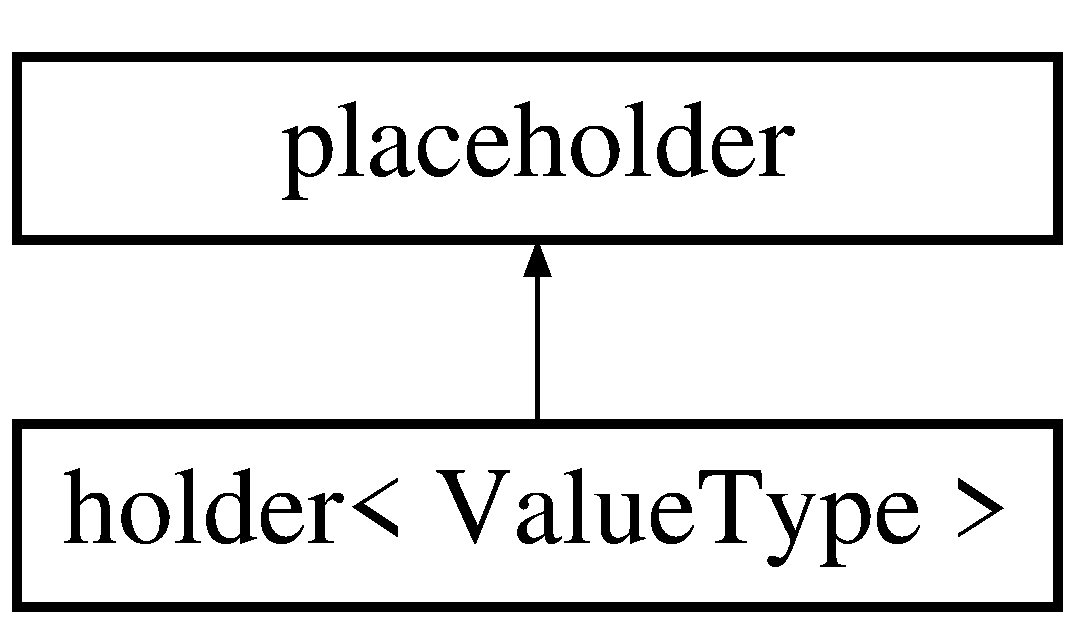
\includegraphics[height=2.000000cm]{dc/d8f/classyuh_1_1any_1_1holder}
\end{center}
\end{figure}
\subsection*{\-Public \-Member \-Functions}
\begin{DoxyCompactItemize}
\item 
\hyperlink{classyuh_1_1any_1_1holder_a4240001abf3fba918bc650ddb5e38239}{holder} (const \-Value\-Type \&value)
\item 
virtual const \-::std\-::type\-\_\-info \& \hyperlink{classyuh_1_1any_1_1holder_a46bcccb2325469ae16d103be16abd4b9}{type} () const 
\item 
virtual \hyperlink{classyuh_1_1any_1_1placeholder}{placeholder} $\ast$ \hyperlink{classyuh_1_1any_1_1holder_a43bd5da15700b27a731a7ec02428eeef}{clone} () const 
\item 
virtual \-::std\-::ostream \& \hyperlink{classyuh_1_1any_1_1holder_ae2b1d2c000a3620614d1dc4d367d073d}{output} (\-::std\-::ostream \&os)
\end{DoxyCompactItemize}
\subsection*{\-Public \-Attributes}
\begin{DoxyCompactItemize}
\item 
\-Value\-Type \hyperlink{classyuh_1_1any_1_1holder_a54a9c5b6e9b85a2a37a16b07905414db}{held}
\end{DoxyCompactItemize}
\subsection*{\-Private \-Member \-Functions}
\begin{DoxyCompactItemize}
\item 
\hyperlink{classyuh_1_1any_1_1holder}{holder} \& \hyperlink{classyuh_1_1any_1_1holder_abde5b12649b80ab7d49fc350d1436850}{operator=} (const \hyperlink{classyuh_1_1any_1_1holder}{holder} \&)
\end{DoxyCompactItemize}


\subsection{\-Detailed \-Description}
\subsubsection*{template$<$typename Value\-Type$>$class yuh\-::any\-::holder$<$ Value\-Type $>$}



\-Definition at line 119 of file any.\-hpp.



\subsection{\-Constructor \& \-Destructor \-Documentation}
\hypertarget{classyuh_1_1any_1_1holder_a4240001abf3fba918bc650ddb5e38239}{\index{yuh\-::any\-::holder@{yuh\-::any\-::holder}!holder@{holder}}
\index{holder@{holder}!yuh::any::holder@{yuh\-::any\-::holder}}
\subsubsection[{holder}]{\setlength{\rightskip}{0pt plus 5cm}{\bf holder} (
\begin{DoxyParamCaption}
\item[{const \-Value\-Type \&}]{value}
\end{DoxyParamCaption}
)\hspace{0.3cm}{\ttfamily  \mbox{[}inline\mbox{]}}}}\label{dc/d8f/classyuh_1_1any_1_1holder_a4240001abf3fba918bc650ddb5e38239}


\-Definition at line 123 of file any.\-hpp.


\begin{DoxyCode}
              : held(value)
            {
            }
\end{DoxyCode}


\subsection{\-Member \-Function \-Documentation}
\hypertarget{classyuh_1_1any_1_1holder_a43bd5da15700b27a731a7ec02428eeef}{\index{yuh\-::any\-::holder@{yuh\-::any\-::holder}!clone@{clone}}
\index{clone@{clone}!yuh::any::holder@{yuh\-::any\-::holder}}
\subsubsection[{clone}]{\setlength{\rightskip}{0pt plus 5cm}virtual {\bf placeholder}$\ast$ {\bf clone} (
\begin{DoxyParamCaption}
{}
\end{DoxyParamCaption}
) const\hspace{0.3cm}{\ttfamily  \mbox{[}inline, virtual\mbox{]}}}}\label{dc/d8f/classyuh_1_1any_1_1holder_a43bd5da15700b27a731a7ec02428eeef}


\-Implements \hyperlink{classyuh_1_1any_1_1placeholder_a1fc9bedc2d9ce8e1f30cd8298bf5427c}{any\-::placeholder}.



\-Definition at line 135 of file any.\-hpp.


\begin{DoxyCode}
            {
                return new holder(held);
            }
\end{DoxyCode}
\hypertarget{classyuh_1_1any_1_1holder_abde5b12649b80ab7d49fc350d1436850}{\index{yuh\-::any\-::holder@{yuh\-::any\-::holder}!operator=@{operator=}}
\index{operator=@{operator=}!yuh::any::holder@{yuh\-::any\-::holder}}
\subsubsection[{operator=}]{\setlength{\rightskip}{0pt plus 5cm}{\bf holder}\& operator= (
\begin{DoxyParamCaption}
\item[{const {\bf holder}$<$ \-Value\-Type $>$ \&}]{}
\end{DoxyParamCaption}
)\hspace{0.3cm}{\ttfamily  \mbox{[}private\mbox{]}}}}\label{dc/d8f/classyuh_1_1any_1_1holder_abde5b12649b80ab7d49fc350d1436850}
\hypertarget{classyuh_1_1any_1_1holder_ae2b1d2c000a3620614d1dc4d367d073d}{\index{yuh\-::any\-::holder@{yuh\-::any\-::holder}!output@{output}}
\index{output@{output}!yuh::any::holder@{yuh\-::any\-::holder}}
\subsubsection[{output}]{\setlength{\rightskip}{0pt plus 5cm}virtual \-::std\-::ostream\& {\bf output} (
\begin{DoxyParamCaption}
\item[{\-::std\-::ostream \&}]{os}
\end{DoxyParamCaption}
)\hspace{0.3cm}{\ttfamily  \mbox{[}inline, virtual\mbox{]}}}}\label{dc/d8f/classyuh_1_1any_1_1holder_ae2b1d2c000a3620614d1dc4d367d073d}


\-Implements \hyperlink{classyuh_1_1any_1_1placeholder_ab55031a8c69345b947e629f9c5306845}{any\-::placeholder}.



\-Definition at line 141 of file any.\-hpp.


\begin{DoxyCode}
            {
                return (os << held);
            }
\end{DoxyCode}
\hypertarget{classyuh_1_1any_1_1holder_a46bcccb2325469ae16d103be16abd4b9}{\index{yuh\-::any\-::holder@{yuh\-::any\-::holder}!type@{type}}
\index{type@{type}!yuh::any::holder@{yuh\-::any\-::holder}}
\subsubsection[{type}]{\setlength{\rightskip}{0pt plus 5cm}virtual const \-::std\-::type\-\_\-info\& {\bf type} (
\begin{DoxyParamCaption}
{}
\end{DoxyParamCaption}
) const\hspace{0.3cm}{\ttfamily  \mbox{[}inline, virtual\mbox{]}}}}\label{dc/d8f/classyuh_1_1any_1_1holder_a46bcccb2325469ae16d103be16abd4b9}


\-Implements \hyperlink{classyuh_1_1any_1_1placeholder_a70b3b61833519a452b860d9f6192fc0d}{any\-::placeholder}.



\-Definition at line 130 of file any.\-hpp.


\begin{DoxyCode}
            {
                return typeid(ValueType);
            }
\end{DoxyCode}


\subsection{\-Member \-Data \-Documentation}
\hypertarget{classyuh_1_1any_1_1holder_a54a9c5b6e9b85a2a37a16b07905414db}{\index{yuh\-::any\-::holder@{yuh\-::any\-::holder}!held@{held}}
\index{held@{held}!yuh::any::holder@{yuh\-::any\-::holder}}
\subsubsection[{held}]{\setlength{\rightskip}{0pt plus 5cm}\-Value\-Type {\bf held}}}\label{dc/d8f/classyuh_1_1any_1_1holder_a54a9c5b6e9b85a2a37a16b07905414db}


\-Definition at line 148 of file any.\-hpp.



\-The documentation for this class was generated from the following file\-:\begin{DoxyCompactItemize}
\item 
include/yuh/\hyperlink{any_8hpp}{any.\-hpp}\end{DoxyCompactItemize}

\hypertarget{structyuh_1_1detail_1_1iterator__tuple}{\section{iterator\-\_\-tuple$<$ \-Args $>$ \-Struct \-Template \-Reference}
\label{dc/d95/structyuh_1_1detail_1_1iterator__tuple}\index{iterator\-\_\-tuple$<$ Args $>$@{iterator\-\_\-tuple$<$ Args $>$}}
}


{\ttfamily \#include $<$cartesian.\-hpp$>$}

\subsection*{\-Public \-Types}
\begin{DoxyCompactItemize}
\item 
typedef \hyperlink{structyuh_1_1detail_1_1iterator__tuple}{iterator\-\_\-tuple}\*
$<$ \hyperlink{structyuh_1_1detail_1_1org__args}{org\-\_\-args}$<$ \-Args...$>$ $>$\-::\hyperlink{structyuh_1_1detail_1_1iterator__tuple_a187957bce48f600bdefd21695e55bde1}{type} \hyperlink{structyuh_1_1detail_1_1iterator__tuple_a187957bce48f600bdefd21695e55bde1}{type}
\end{DoxyCompactItemize}


\subsection{\-Detailed \-Description}
\subsubsection*{template$<$typename... \-Args$>$struct yuh\-::detail\-::iterator\-\_\-tuple$<$ Args $>$}



\-Definition at line 41 of file cartesian.\-hpp.



\subsection{\-Member \-Typedef \-Documentation}
\hypertarget{structyuh_1_1detail_1_1iterator__tuple_a187957bce48f600bdefd21695e55bde1}{\index{yuh\-::detail\-::iterator\-\_\-tuple@{yuh\-::detail\-::iterator\-\_\-tuple}!type@{type}}
\index{type@{type}!yuh::detail::iterator_tuple@{yuh\-::detail\-::iterator\-\_\-tuple}}
\subsubsection[{type}]{\setlength{\rightskip}{0pt plus 5cm}typedef {\bf iterator\-\_\-tuple}$<${\bf org\-\_\-args}$<$\-Args...$>$ $>$\-::{\bf type} {\bf type}}}\label{dc/d95/structyuh_1_1detail_1_1iterator__tuple_a187957bce48f600bdefd21695e55bde1}


\-Definition at line 43 of file cartesian.\-hpp.



\-The documentation for this struct was generated from the following file\-:\begin{DoxyCompactItemize}
\item 
include/yuh/\hyperlink{cartesian_8hpp}{cartesian.\-hpp}\end{DoxyCompactItemize}

\hypertarget{structyuh_1_1detail_1_1iterator__tuple_3_01org__args_3_01T_00_01Org_8_8_8_4_00_01Args_8_8_8_4}{\section{iterator\-\_\-tuple$<$ org\-\_\-args$<$ \-T, \-Org...$>$, \-Args...$>$ \-Struct \-Template \-Reference}
\label{d2/de2/structyuh_1_1detail_1_1iterator__tuple_3_01org__args_3_01T_00_01Org_8_8_8_4_00_01Args_8_8_8_4}\index{iterator\-\_\-tuple$<$ org\-\_\-args$<$ T, Org...$>$, Args...$>$@{iterator\-\_\-tuple$<$ org\-\_\-args$<$ T, Org...$>$, Args...$>$}}
}


{\ttfamily \#include $<$cartesian.\-hpp$>$}

\subsection*{\-Public \-Types}
\begin{DoxyCompactItemize}
\item 
typedef \hyperlink{structyuh_1_1detail_1_1iterator__tuple}{iterator\-\_\-tuple}\*
$<$ \hyperlink{structyuh_1_1detail_1_1org__args}{org\-\_\-args}$<$ \-Org...$>$, \-Args..., \*
typename boost\-::range\-\_\-iterator\*
$<$ \-T $>$\-::\hyperlink{structyuh_1_1detail_1_1iterator__tuple_3_01org__args_3_01T_00_01Org_8_8_8_4_00_01Args_8_8_8_4_a22487632bf6ac08da23ab56b24fcd551}{type} $>$\-::\hyperlink{structyuh_1_1detail_1_1iterator__tuple_3_01org__args_3_01T_00_01Org_8_8_8_4_00_01Args_8_8_8_4_a22487632bf6ac08da23ab56b24fcd551}{type} \hyperlink{structyuh_1_1detail_1_1iterator__tuple_3_01org__args_3_01T_00_01Org_8_8_8_4_00_01Args_8_8_8_4_a22487632bf6ac08da23ab56b24fcd551}{type}
\end{DoxyCompactItemize}


\subsection{\-Detailed \-Description}
\subsubsection*{template$<$typename T, typename... \-Org, typename... \-Args$>$struct yuh\-::detail\-::iterator\-\_\-tuple$<$ org\-\_\-args$<$ T, Org...$>$, Args...$>$}



\-Definition at line 46 of file cartesian.\-hpp.



\subsection{\-Member \-Typedef \-Documentation}
\hypertarget{structyuh_1_1detail_1_1iterator__tuple_3_01org__args_3_01T_00_01Org_8_8_8_4_00_01Args_8_8_8_4_a22487632bf6ac08da23ab56b24fcd551}{\index{yuh\-::detail\-::iterator\-\_\-tuple$<$ org\-\_\-args$<$ T, Org...$>$, Args...$>$@{yuh\-::detail\-::iterator\-\_\-tuple$<$ org\-\_\-args$<$ T, Org...$>$, Args...$>$}!type@{type}}
\index{type@{type}!yuh::detail::iterator_tuple< org_args< T, Org...>, Args...>@{yuh\-::detail\-::iterator\-\_\-tuple$<$ org\-\_\-args$<$ T, Org...$>$, Args...$>$}}
\subsubsection[{type}]{\setlength{\rightskip}{0pt plus 5cm}typedef {\bf iterator\-\_\-tuple}$<$ {\bf org\-\_\-args}$<$\-Org...$>$, \-Args..., typename boost\-::range\-\_\-iterator$<$ \-T $>$\-::{\bf type} $>$\-::{\bf type} {\bf type}}}\label{d2/de2/structyuh_1_1detail_1_1iterator__tuple_3_01org__args_3_01T_00_01Org_8_8_8_4_00_01Args_8_8_8_4_a22487632bf6ac08da23ab56b24fcd551}


\-Definition at line 52 of file cartesian.\-hpp.



\-The documentation for this struct was generated from the following file\-:\begin{DoxyCompactItemize}
\item 
include/yuh/\hyperlink{cartesian_8hpp}{cartesian.\-hpp}\end{DoxyCompactItemize}

\hypertarget{structyuh_1_1detail_1_1iterator__tuple_3_01org__args_3_4_00_01Args_8_8_8_4}{\section{iterator\-\_\-tuple$<$ org\-\_\-args$<$$>$, \-Args...$>$ \-Struct \-Template \-Reference}
\label{da/d79/structyuh_1_1detail_1_1iterator__tuple_3_01org__args_3_4_00_01Args_8_8_8_4}\index{iterator\-\_\-tuple$<$ org\-\_\-args$<$$>$, Args...$>$@{iterator\-\_\-tuple$<$ org\-\_\-args$<$$>$, Args...$>$}}
}


{\ttfamily \#include $<$cartesian.\-hpp$>$}

\subsection*{\-Public \-Types}
\begin{DoxyCompactItemize}
\item 
typedef std\-::tuple$<$ \-Args...$>$ \hyperlink{structyuh_1_1detail_1_1iterator__tuple_3_01org__args_3_4_00_01Args_8_8_8_4_a0c208c6f55e889b43018b13a7aa6a8da}{type}
\end{DoxyCompactItemize}


\subsection{\-Detailed \-Description}
\subsubsection*{template$<$typename... \-Args$>$struct yuh\-::detail\-::iterator\-\_\-tuple$<$ org\-\_\-args$<$$>$, Args...$>$}



\-Definition at line 55 of file cartesian.\-hpp.



\subsection{\-Member \-Typedef \-Documentation}
\hypertarget{structyuh_1_1detail_1_1iterator__tuple_3_01org__args_3_4_00_01Args_8_8_8_4_a0c208c6f55e889b43018b13a7aa6a8da}{\index{yuh\-::detail\-::iterator\-\_\-tuple$<$ org\-\_\-args$<$$>$, Args...$>$@{yuh\-::detail\-::iterator\-\_\-tuple$<$ org\-\_\-args$<$$>$, Args...$>$}!type@{type}}
\index{type@{type}!yuh::detail::iterator_tuple< org_args<>, Args...>@{yuh\-::detail\-::iterator\-\_\-tuple$<$ org\-\_\-args$<$$>$, Args...$>$}}
\subsubsection[{type}]{\setlength{\rightskip}{0pt plus 5cm}typedef std\-::tuple$<$\-Args...$>$ {\bf type}}}\label{da/d79/structyuh_1_1detail_1_1iterator__tuple_3_01org__args_3_4_00_01Args_8_8_8_4_a0c208c6f55e889b43018b13a7aa6a8da}


\-Definition at line 57 of file cartesian.\-hpp.



\-The documentation for this struct was generated from the following file\-:\begin{DoxyCompactItemize}
\item 
include/yuh/\hyperlink{cartesian_8hpp}{cartesian.\-hpp}\end{DoxyCompactItemize}

\hypertarget{classyuh_1_1detail_1_1logger}{\section{logger \-Class \-Reference}
\label{d1/dce/classyuh_1_1detail_1_1logger}\index{logger@{logger}}
}


{\ttfamily \#include $<$logger.\-h$>$}

\subsection*{\-Public \-Member \-Functions}
\begin{DoxyCompactItemize}
\item 
\hyperlink{classyuh_1_1detail_1_1logger_abc46b52b3bf194874ba4ebd9c415415a}{$\sim$logger} ()
\item 
{\footnotesize template$<$typename T $>$ }\\\hyperlink{classyuh_1_1detail_1_1logger}{logger} \& \hyperlink{classyuh_1_1detail_1_1logger_ac0b044fa4008d42252e0342a7a83461f}{operator()} (int n, \-T const \&data)
\end{DoxyCompactItemize}
\subsection*{\-Private \-Member \-Functions}
\begin{DoxyCompactItemize}
\item 
\hyperlink{classyuh_1_1detail_1_1logger_a97e3b3adabf67bc7d3650ed14214ddaa}{logger} ()
\item 
{\footnotesize template$<$typename Range $>$ }\\\hyperlink{classyuh_1_1detail_1_1logger_ab5ad71f6923679744edb73c33af936ca}{logger} (\-Range \&rng, int interval\-\_\-milliseconds=100)
\item 
\hyperlink{classyuh_1_1detail_1_1logger_a96bb29b740d2079eff2a343b96ba8fe6}{logger} (const \hyperlink{classyuh_1_1detail_1_1logger}{logger} \&)
\item 
\hyperlink{classyuh_1_1detail_1_1logger_a9a213af89763057907f1d6c5a65d9eae}{logger} (\hyperlink{classyuh_1_1detail_1_1logger}{logger} \&\&)
\item 
\hyperlink{classyuh_1_1detail_1_1logger}{logger} \& \hyperlink{classyuh_1_1detail_1_1logger_aeadd53088e5adb387e95cdcfb5301a06}{operator=} (const \hyperlink{classyuh_1_1detail_1_1logger}{logger} \&)
\item 
\hyperlink{classyuh_1_1detail_1_1logger}{logger} \& \hyperlink{classyuh_1_1detail_1_1logger_a99e78de8d2b06cf46095a56c4b607e42}{operator=} (\hyperlink{classyuh_1_1detail_1_1logger}{logger} \&\&)
\item 
void \hyperlink{classyuh_1_1detail_1_1logger_aaab9f2249ce35dc29648607974a17cc9}{thread\-\_\-loop} ()
\item 
void \hyperlink{classyuh_1_1detail_1_1logger_a7437b254e19e7e12fc2ec99945f4ecea}{output} ()
\end{DoxyCompactItemize}
\subsection*{\-Private \-Attributes}
\begin{DoxyCompactItemize}
\item 
std\-::vector$<$ \hyperlink{classyuh_1_1thread__queue}{thread\-\_\-queue}$<$ \hyperlink{classyuh_1_1any}{any} $>$ $>$ \hyperlink{classyuh_1_1detail_1_1logger_af2b7d7f50e13fa5e21ae7dbaaaf56d81}{q\-\_\-}
\item 
std\-::vector$<$ std\-::ofstream $>$ \hyperlink{classyuh_1_1detail_1_1logger_a281aed45a8c2b369a0e5965cdb00c273}{ofs\-\_\-}
\item 
boost\-::chrono\-::milliseconds \hyperlink{classyuh_1_1detail_1_1logger_a2ae4364eadd2ae03f6ffb965d0622d21}{interval\-\_\-}
\item 
std\-::atomic$<$ bool $>$ \hyperlink{classyuh_1_1detail_1_1logger_a91290cb294b9bbefd56c3a97bf00dcab}{end\-\_\-flag\-\_\-}
\item 
boost\-::thread \hyperlink{classyuh_1_1detail_1_1logger_a813cb749320df26fae57fc171a765178}{thread\-\_\-}
\end{DoxyCompactItemize}
\subsection*{\-Friends}
\begin{DoxyCompactItemize}
\item 
class \hyperlink{classyuh_1_1detail_1_1logger_a697b2e01800239e686ae61d7129fb769}{\-V\-S\-Test\-::logger\-\_\-unittest}
\item 
class \hyperlink{classyuh_1_1detail_1_1logger_a568e0733d4add58a1c20947fbc9f8ad5}{singleton$<$ logger $>$}
\end{DoxyCompactItemize}


\subsection{\-Detailed \-Description}
ログ 

\-Definition at line 31 of file logger.\-h.



\subsection{\-Constructor \& \-Destructor \-Documentation}
\hypertarget{classyuh_1_1detail_1_1logger_abc46b52b3bf194874ba4ebd9c415415a}{\index{yuh\-::detail\-::logger@{yuh\-::detail\-::logger}!$\sim$logger@{$\sim$logger}}
\index{$\sim$logger@{$\sim$logger}!yuh::detail::logger@{yuh\-::detail\-::logger}}
\subsubsection[{$\sim$logger}]{\setlength{\rightskip}{0pt plus 5cm}$\sim${\bf logger} (
\begin{DoxyParamCaption}
{}
\end{DoxyParamCaption}
)}}\label{d1/dce/classyuh_1_1detail_1_1logger_abc46b52b3bf194874ba4ebd9c415415a}


\-Definition at line 25 of file logger.\-cpp.


\begin{DoxyCode}
        {
            end_flag_ = false;
            thread_.join(); //ここで停止

            //後処理
            output();
            boost::for_each(
                ofs_, 
                [](std::ofstream& ofs){ ofs.close(); }
            );
        }
\end{DoxyCode}
\hypertarget{classyuh_1_1detail_1_1logger_a97e3b3adabf67bc7d3650ed14214ddaa}{\index{yuh\-::detail\-::logger@{yuh\-::detail\-::logger}!logger@{logger}}
\index{logger@{logger}!yuh::detail::logger@{yuh\-::detail\-::logger}}
\subsubsection[{logger}]{\setlength{\rightskip}{0pt plus 5cm}{\bf logger} (
\begin{DoxyParamCaption}
{}
\end{DoxyParamCaption}
)\hspace{0.3cm}{\ttfamily  \mbox{[}private\mbox{]}}}}\label{d1/dce/classyuh_1_1detail_1_1logger_a97e3b3adabf67bc7d3650ed14214ddaa}


\-Definition at line 14 of file logger.\-cpp.


\begin{DoxyCode}
            : q_()
            , ofs_()
            , interval_(100)
            , end_flag_(true)
            , thread_()
        {
            thread_ = boost::thread(&logger::thread_loop, this); //move
        }
\end{DoxyCode}
\hypertarget{classyuh_1_1detail_1_1logger_ab5ad71f6923679744edb73c33af936ca}{\index{yuh\-::detail\-::logger@{yuh\-::detail\-::logger}!logger@{logger}}
\index{logger@{logger}!yuh::detail::logger@{yuh\-::detail\-::logger}}
\subsubsection[{logger}]{\setlength{\rightskip}{0pt plus 5cm}{\bf logger} (
\begin{DoxyParamCaption}
\item[{\-Range \&}]{rng, }
\item[{int}]{interval\-\_\-milliseconds = {\ttfamily 100}}
\end{DoxyParamCaption}
)\hspace{0.3cm}{\ttfamily  \mbox{[}private\mbox{]}}}}\label{d1/dce/classyuh_1_1detail_1_1logger_ab5ad71f6923679744edb73c33af936ca}
ctor 
\begin{DoxyParams}{\-Parameters}
{\em rng} & 出力先ファイル名リスト \\
\hline
{\em interval\-\_\-milliseconds} & 出力チェック間隔 \\
\hline
\end{DoxyParams}


\-Definition at line 101 of file logger.\-h.


\begin{DoxyCode}
            : q_(boost::size(filenames))
            , ofs_(0)
            , interval_(interval_milliseconds)
            , end_flag_(true)
            , thread_()
        {
            ofs_.reserve(q_.size());
            boost::for_each(
                filenames, 
                [&](std::string const& str) { 
                    auto p = boost::filesystem::absolute(
      boost::filesystem::path(str));
                    if ( !boost::filesystem::exists(p.parent_path()) )
                        boost::filesystem::create_directories(p.parent_path());

                    ofs_.emplace_back(p.string()); 
            }
            );

            thread_ = boost::thread(&logger::thread_loop, this); 
        }
\end{DoxyCode}
\hypertarget{classyuh_1_1detail_1_1logger_a96bb29b740d2079eff2a343b96ba8fe6}{\index{yuh\-::detail\-::logger@{yuh\-::detail\-::logger}!logger@{logger}}
\index{logger@{logger}!yuh::detail::logger@{yuh\-::detail\-::logger}}
\subsubsection[{logger}]{\setlength{\rightskip}{0pt plus 5cm}{\bf logger} (
\begin{DoxyParamCaption}
\item[{const {\bf logger} \&}]{}
\end{DoxyParamCaption}
)\hspace{0.3cm}{\ttfamily  \mbox{[}private\mbox{]}}}}\label{d1/dce/classyuh_1_1detail_1_1logger_a96bb29b740d2079eff2a343b96ba8fe6}
\hypertarget{classyuh_1_1detail_1_1logger_a9a213af89763057907f1d6c5a65d9eae}{\index{yuh\-::detail\-::logger@{yuh\-::detail\-::logger}!logger@{logger}}
\index{logger@{logger}!yuh::detail::logger@{yuh\-::detail\-::logger}}
\subsubsection[{logger}]{\setlength{\rightskip}{0pt plus 5cm}{\bf logger} (
\begin{DoxyParamCaption}
\item[{{\bf logger} \&\&}]{}
\end{DoxyParamCaption}
)\hspace{0.3cm}{\ttfamily  \mbox{[}private\mbox{]}}}}\label{d1/dce/classyuh_1_1detail_1_1logger_a9a213af89763057907f1d6c5a65d9eae}


\subsection{\-Member \-Function \-Documentation}
\hypertarget{classyuh_1_1detail_1_1logger_ac0b044fa4008d42252e0342a7a83461f}{\index{yuh\-::detail\-::logger@{yuh\-::detail\-::logger}!operator()@{operator()}}
\index{operator()@{operator()}!yuh::detail::logger@{yuh\-::detail\-::logger}}
\subsubsection[{operator()}]{\setlength{\rightskip}{0pt plus 5cm}{\bf logger} \& operator() (
\begin{DoxyParamCaption}
\item[{int}]{n, }
\item[{\-T const \&}]{data}
\end{DoxyParamCaption}
)}}\label{d1/dce/classyuh_1_1detail_1_1logger_ac0b044fa4008d42252e0342a7a83461f}
出力queueにpush 
\begin{DoxyParams}{\-Parameters}
{\em n} & queue番号 \\
\hline
{\em data} & 出力データ ストリーム出力operator$<$$<$に対応していればなんでも \\
\hline
\end{DoxyParams}
\begin{DoxyReturn}{\-Returns}
自身 ()を連結していける 
\end{DoxyReturn}


\-Definition at line 124 of file logger.\-h.


\begin{DoxyCode}
        {
            q_[n].push(data);
            return *this;
        }
\end{DoxyCode}
\hypertarget{classyuh_1_1detail_1_1logger_aeadd53088e5adb387e95cdcfb5301a06}{\index{yuh\-::detail\-::logger@{yuh\-::detail\-::logger}!operator=@{operator=}}
\index{operator=@{operator=}!yuh::detail::logger@{yuh\-::detail\-::logger}}
\subsubsection[{operator=}]{\setlength{\rightskip}{0pt plus 5cm}{\bf logger}\& operator= (
\begin{DoxyParamCaption}
\item[{const {\bf logger} \&}]{}
\end{DoxyParamCaption}
)\hspace{0.3cm}{\ttfamily  \mbox{[}private\mbox{]}}}}\label{d1/dce/classyuh_1_1detail_1_1logger_aeadd53088e5adb387e95cdcfb5301a06}
\hypertarget{classyuh_1_1detail_1_1logger_a99e78de8d2b06cf46095a56c4b607e42}{\index{yuh\-::detail\-::logger@{yuh\-::detail\-::logger}!operator=@{operator=}}
\index{operator=@{operator=}!yuh::detail::logger@{yuh\-::detail\-::logger}}
\subsubsection[{operator=}]{\setlength{\rightskip}{0pt plus 5cm}{\bf logger}\& operator= (
\begin{DoxyParamCaption}
\item[{{\bf logger} \&\&}]{}
\end{DoxyParamCaption}
)\hspace{0.3cm}{\ttfamily  \mbox{[}private\mbox{]}}}}\label{d1/dce/classyuh_1_1detail_1_1logger_a99e78de8d2b06cf46095a56c4b607e42}
\hypertarget{classyuh_1_1detail_1_1logger_a7437b254e19e7e12fc2ec99945f4ecea}{\index{yuh\-::detail\-::logger@{yuh\-::detail\-::logger}!output@{output}}
\index{output@{output}!yuh::detail::logger@{yuh\-::detail\-::logger}}
\subsubsection[{output}]{\setlength{\rightskip}{0pt plus 5cm}void {\bf output} (
\begin{DoxyParamCaption}
{}
\end{DoxyParamCaption}
)\hspace{0.3cm}{\ttfamily  \mbox{[}private\mbox{]}}}}\label{d1/dce/classyuh_1_1detail_1_1logger_a7437b254e19e7e12fc2ec99945f4ecea}
内部用出力処理 

\-Definition at line 38 of file logger.\-cpp.


\begin{DoxyCode}
        {
            for( auto t: boost::combine(q_, ofs_) )
            {
                auto& q = boost::get<0>(t);
                auto& ofs = boost::get<1>(t);
                while(!q.empty())
                {
                    ofs << q.front() << std::endl;
                    q.pop();
                }
            }
        }
\end{DoxyCode}
\hypertarget{classyuh_1_1detail_1_1logger_aaab9f2249ce35dc29648607974a17cc9}{\index{yuh\-::detail\-::logger@{yuh\-::detail\-::logger}!thread\-\_\-loop@{thread\-\_\-loop}}
\index{thread\-\_\-loop@{thread\-\_\-loop}!yuh::detail::logger@{yuh\-::detail\-::logger}}
\subsubsection[{thread\-\_\-loop}]{\setlength{\rightskip}{0pt plus 5cm}void {\bf thread\-\_\-loop} (
\begin{DoxyParamCaption}
{}
\end{DoxyParamCaption}
)\hspace{0.3cm}{\ttfamily  \mbox{[}private\mbox{]}}}}\label{d1/dce/classyuh_1_1detail_1_1logger_aaab9f2249ce35dc29648607974a17cc9}
ループ関数 bgで出力していく 

\-Definition at line 52 of file logger.\-cpp.


\begin{DoxyCode}
        {
            while(end_flag_)
            {
                //メイン処理
                output();

                boost::this_thread::sleep_for(interval_);
            }
        }
\end{DoxyCode}


\subsection{\-Friends \-And \-Related \-Function \-Documentation}
\hypertarget{classyuh_1_1detail_1_1logger_a568e0733d4add58a1c20947fbc9f8ad5}{\index{yuh\-::detail\-::logger@{yuh\-::detail\-::logger}!singleton$<$ logger $>$@{singleton$<$ logger $>$}}
\index{singleton$<$ logger $>$@{singleton$<$ logger $>$}!yuh::detail::logger@{yuh\-::detail\-::logger}}
\subsubsection[{singleton$<$ logger $>$}]{\setlength{\rightskip}{0pt plus 5cm}friend class {\bf singleton}$<$ {\bf logger} $>$\hspace{0.3cm}{\ttfamily  \mbox{[}friend\mbox{]}}}}\label{d1/dce/classyuh_1_1detail_1_1logger_a568e0733d4add58a1c20947fbc9f8ad5}


\-Definition at line 97 of file logger.\-h.

\hypertarget{classyuh_1_1detail_1_1logger_a697b2e01800239e686ae61d7129fb769}{\index{yuh\-::detail\-::logger@{yuh\-::detail\-::logger}!\-V\-S\-Test\-::logger\-\_\-unittest@{\-V\-S\-Test\-::logger\-\_\-unittest}}
\index{\-V\-S\-Test\-::logger\-\_\-unittest@{\-V\-S\-Test\-::logger\-\_\-unittest}!yuh::detail::logger@{yuh\-::detail\-::logger}}
\subsubsection[{\-V\-S\-Test\-::logger\-\_\-unittest}]{\setlength{\rightskip}{0pt plus 5cm}friend class \-V\-S\-Test\-::logger\-\_\-unittest\hspace{0.3cm}{\ttfamily  \mbox{[}friend\mbox{]}}}}\label{d1/dce/classyuh_1_1detail_1_1logger_a697b2e01800239e686ae61d7129fb769}


\-Definition at line 95 of file logger.\-h.



\subsection{\-Member \-Data \-Documentation}
\hypertarget{classyuh_1_1detail_1_1logger_a91290cb294b9bbefd56c3a97bf00dcab}{\index{yuh\-::detail\-::logger@{yuh\-::detail\-::logger}!end\-\_\-flag\-\_\-@{end\-\_\-flag\-\_\-}}
\index{end\-\_\-flag\-\_\-@{end\-\_\-flag\-\_\-}!yuh::detail::logger@{yuh\-::detail\-::logger}}
\subsubsection[{end\-\_\-flag\-\_\-}]{\setlength{\rightskip}{0pt plus 5cm}std\-::atomic$<$bool$>$ {\bf end\-\_\-flag\-\_\-}\hspace{0.3cm}{\ttfamily  \mbox{[}private\mbox{]}}}}\label{d1/dce/classyuh_1_1detail_1_1logger_a91290cb294b9bbefd56c3a97bf00dcab}
スレッド終了フラグ 

\-Definition at line 88 of file logger.\-h.

\hypertarget{classyuh_1_1detail_1_1logger_a2ae4364eadd2ae03f6ffb965d0622d21}{\index{yuh\-::detail\-::logger@{yuh\-::detail\-::logger}!interval\-\_\-@{interval\-\_\-}}
\index{interval\-\_\-@{interval\-\_\-}!yuh::detail::logger@{yuh\-::detail\-::logger}}
\subsubsection[{interval\-\_\-}]{\setlength{\rightskip}{0pt plus 5cm}boost\-::chrono\-::milliseconds {\bf interval\-\_\-}\hspace{0.3cm}{\ttfamily  \mbox{[}private\mbox{]}}}}\label{d1/dce/classyuh_1_1detail_1_1logger_a2ae4364eadd2ae03f6ffb965d0622d21}
チェック待機時間 

\-Definition at line 84 of file logger.\-h.

\hypertarget{classyuh_1_1detail_1_1logger_a281aed45a8c2b369a0e5965cdb00c273}{\index{yuh\-::detail\-::logger@{yuh\-::detail\-::logger}!ofs\-\_\-@{ofs\-\_\-}}
\index{ofs\-\_\-@{ofs\-\_\-}!yuh::detail::logger@{yuh\-::detail\-::logger}}
\subsubsection[{ofs\-\_\-}]{\setlength{\rightskip}{0pt plus 5cm}std\-::vector$<$std\-::ofstream$>$ {\bf ofs\-\_\-}\hspace{0.3cm}{\ttfamily  \mbox{[}private\mbox{]}}}}\label{d1/dce/classyuh_1_1detail_1_1logger_a281aed45a8c2b369a0e5965cdb00c273}
出力ストリームリスト 

\-Definition at line 79 of file logger.\-h.

\hypertarget{classyuh_1_1detail_1_1logger_af2b7d7f50e13fa5e21ae7dbaaaf56d81}{\index{yuh\-::detail\-::logger@{yuh\-::detail\-::logger}!q\-\_\-@{q\-\_\-}}
\index{q\-\_\-@{q\-\_\-}!yuh::detail::logger@{yuh\-::detail\-::logger}}
\subsubsection[{q\-\_\-}]{\setlength{\rightskip}{0pt plus 5cm}std\-::vector$<${\bf thread\-\_\-queue}$<${\bf any}$>$ $>$ {\bf q\-\_\-}\hspace{0.3cm}{\ttfamily  \mbox{[}private\mbox{]}}}}\label{d1/dce/classyuh_1_1detail_1_1logger_af2b7d7f50e13fa5e21ae7dbaaaf56d81}
出力用queueリスト 

\-Definition at line 75 of file logger.\-h.

\hypertarget{classyuh_1_1detail_1_1logger_a813cb749320df26fae57fc171a765178}{\index{yuh\-::detail\-::logger@{yuh\-::detail\-::logger}!thread\-\_\-@{thread\-\_\-}}
\index{thread\-\_\-@{thread\-\_\-}!yuh::detail::logger@{yuh\-::detail\-::logger}}
\subsubsection[{thread\-\_\-}]{\setlength{\rightskip}{0pt plus 5cm}boost\-::thread {\bf thread\-\_\-}\hspace{0.3cm}{\ttfamily  \mbox{[}private\mbox{]}}}}\label{d1/dce/classyuh_1_1detail_1_1logger_a813cb749320df26fae57fc171a765178}
スレッド 

\-Definition at line 92 of file logger.\-h.



\-The documentation for this class was generated from the following files\-:\begin{DoxyCompactItemize}
\item 
include/yuh/\hyperlink{logger_8h}{logger.\-h}\item 
src/\hyperlink{logger_8cpp}{logger.\-cpp}\end{DoxyCompactItemize}

\hypertarget{structyuh_1_1detail_1_1org__args}{\section{org\-\_\-args$<$ \-Args $>$ \-Struct \-Template \-Reference}
\label{d6/d2b/structyuh_1_1detail_1_1org__args}\index{org\-\_\-args$<$ Args $>$@{org\-\_\-args$<$ Args $>$}}
}


{\ttfamily \#include $<$cartesian.\-hpp$>$}



\subsection{\-Detailed \-Description}
\subsubsection*{template$<$typename... \-Args$>$struct yuh\-::detail\-::org\-\_\-args$<$ Args $>$}



\-Definition at line 12 of file cartesian.\-hpp.



\-The documentation for this struct was generated from the following file\-:\begin{DoxyCompactItemize}
\item 
include/yuh/\hyperlink{cartesian_8hpp}{cartesian.\-hpp}\end{DoxyCompactItemize}

\hypertarget{classyuh_1_1any_1_1placeholder}{\section{any\-:\-:placeholder \-Class \-Reference}
\label{dc/de9/classyuh_1_1any_1_1placeholder}\index{any\-::placeholder@{any\-::placeholder}}
}
\-Inheritance diagram for any\-:\-:placeholder\-:\begin{figure}[H]
\begin{center}
\leavevmode
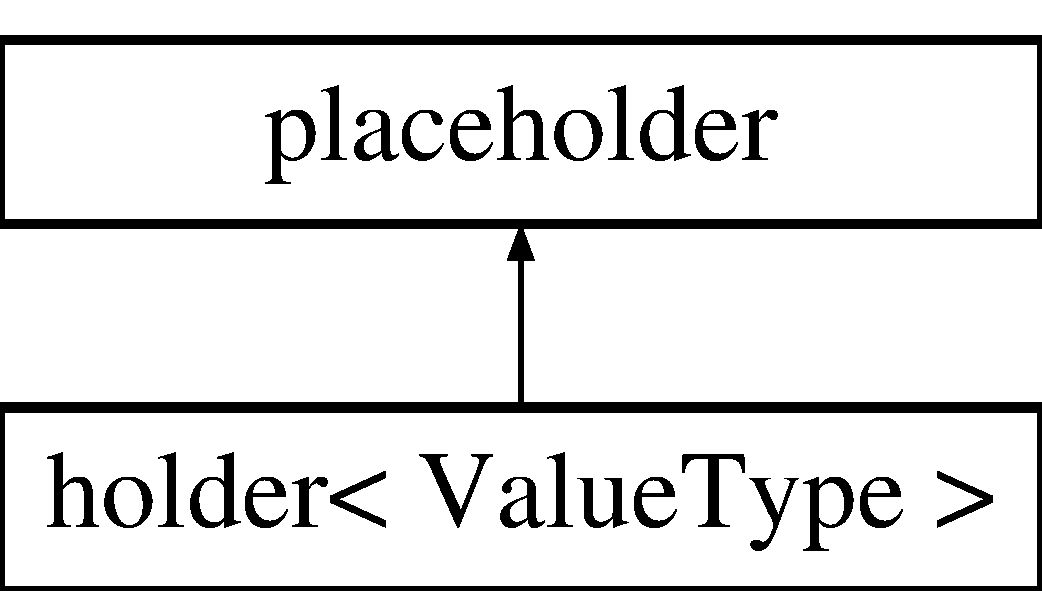
\includegraphics[height=2.000000cm]{dc/de9/classyuh_1_1any_1_1placeholder}
\end{center}
\end{figure}
\subsection*{\-Public \-Member \-Functions}
\begin{DoxyCompactItemize}
\item 
virtual \hyperlink{classyuh_1_1any_1_1placeholder_a977806fe3807787ff8d8c27116fa7ac2}{$\sim$placeholder} ()
\item 
virtual const \-::std\-::type\-\_\-info \& \hyperlink{classyuh_1_1any_1_1placeholder_a70b3b61833519a452b860d9f6192fc0d}{type} () const =0
\item 
virtual \hyperlink{classyuh_1_1any_1_1placeholder}{placeholder} $\ast$ \hyperlink{classyuh_1_1any_1_1placeholder_a1fc9bedc2d9ce8e1f30cd8298bf5427c}{clone} () const =0
\item 
virtual \-::std\-::ostream \& \hyperlink{classyuh_1_1any_1_1placeholder_ab55031a8c69345b947e629f9c5306845}{output} (\-::std\-::ostream \&os)=0
\end{DoxyCompactItemize}


\subsection{\-Detailed \-Description}


\-Definition at line 100 of file any.\-hpp.



\subsection{\-Constructor \& \-Destructor \-Documentation}
\hypertarget{classyuh_1_1any_1_1placeholder_a977806fe3807787ff8d8c27116fa7ac2}{\index{yuh\-::any\-::placeholder@{yuh\-::any\-::placeholder}!$\sim$placeholder@{$\sim$placeholder}}
\index{$\sim$placeholder@{$\sim$placeholder}!yuh::any::placeholder@{yuh\-::any\-::placeholder}}
\subsubsection[{$\sim$placeholder}]{\setlength{\rightskip}{0pt plus 5cm}virtual $\sim${\bf placeholder} (
\begin{DoxyParamCaption}
{}
\end{DoxyParamCaption}
)\hspace{0.3cm}{\ttfamily  \mbox{[}inline, virtual\mbox{]}}}}\label{dc/de9/classyuh_1_1any_1_1placeholder_a977806fe3807787ff8d8c27116fa7ac2}


\-Definition at line 104 of file any.\-hpp.


\begin{DoxyCode}
            {
            }
\end{DoxyCode}


\subsection{\-Member \-Function \-Documentation}
\hypertarget{classyuh_1_1any_1_1placeholder_a1fc9bedc2d9ce8e1f30cd8298bf5427c}{\index{yuh\-::any\-::placeholder@{yuh\-::any\-::placeholder}!clone@{clone}}
\index{clone@{clone}!yuh::any::placeholder@{yuh\-::any\-::placeholder}}
\subsubsection[{clone}]{\setlength{\rightskip}{0pt plus 5cm}virtual {\bf placeholder}$\ast$ {\bf clone} (
\begin{DoxyParamCaption}
{}
\end{DoxyParamCaption}
) const\hspace{0.3cm}{\ttfamily  \mbox{[}pure virtual\mbox{]}}}}\label{dc/de9/classyuh_1_1any_1_1placeholder_a1fc9bedc2d9ce8e1f30cd8298bf5427c}


\-Implemented in \hyperlink{classyuh_1_1any_1_1holder_a43bd5da15700b27a731a7ec02428eeef}{any\-::holder$<$ Value\-Type $>$}.

\hypertarget{classyuh_1_1any_1_1placeholder_ab55031a8c69345b947e629f9c5306845}{\index{yuh\-::any\-::placeholder@{yuh\-::any\-::placeholder}!output@{output}}
\index{output@{output}!yuh::any::placeholder@{yuh\-::any\-::placeholder}}
\subsubsection[{output}]{\setlength{\rightskip}{0pt plus 5cm}virtual \-::std\-::ostream\& {\bf output} (
\begin{DoxyParamCaption}
\item[{\-::std\-::ostream \&}]{os}
\end{DoxyParamCaption}
)\hspace{0.3cm}{\ttfamily  \mbox{[}pure virtual\mbox{]}}}}\label{dc/de9/classyuh_1_1any_1_1placeholder_ab55031a8c69345b947e629f9c5306845}


\-Implemented in \hyperlink{classyuh_1_1any_1_1holder_ae2b1d2c000a3620614d1dc4d367d073d}{any\-::holder$<$ Value\-Type $>$}.

\hypertarget{classyuh_1_1any_1_1placeholder_a70b3b61833519a452b860d9f6192fc0d}{\index{yuh\-::any\-::placeholder@{yuh\-::any\-::placeholder}!type@{type}}
\index{type@{type}!yuh::any::placeholder@{yuh\-::any\-::placeholder}}
\subsubsection[{type}]{\setlength{\rightskip}{0pt plus 5cm}virtual const \-::std\-::type\-\_\-info\& {\bf type} (
\begin{DoxyParamCaption}
{}
\end{DoxyParamCaption}
) const\hspace{0.3cm}{\ttfamily  \mbox{[}pure virtual\mbox{]}}}}\label{dc/de9/classyuh_1_1any_1_1placeholder_a70b3b61833519a452b860d9f6192fc0d}


\-Implemented in \hyperlink{classyuh_1_1any_1_1holder_a46bcccb2325469ae16d103be16abd4b9}{any\-::holder$<$ Value\-Type $>$}.



\-The documentation for this class was generated from the following file\-:\begin{DoxyCompactItemize}
\item 
include/yuh/\hyperlink{any_8hpp}{any.\-hpp}\end{DoxyCompactItemize}

\hypertarget{classyuh_1_1range__detail_1_1polygonal__iterator}{\section{polygonal\-\_\-iterator$<$ \-P, \-Integer $>$ \-Class \-Template \-Reference}
\label{d9/d0c/classyuh_1_1range__detail_1_1polygonal__iterator}\index{polygonal\-\_\-iterator$<$ P, Integer $>$@{polygonal\-\_\-iterator$<$ P, Integer $>$}}
}


{\ttfamily \#include $<$polygonal.\-hpp$>$}

\subsection*{\-Public \-Types}
\begin{DoxyCompactItemize}
\item 
typedef base\-\_\-t\-::value\-\_\-type \hyperlink{classyuh_1_1range__detail_1_1polygonal__iterator_ab7468d4ed49b58c84d6c1b71779fb43e}{value\-\_\-type}
\item 
typedef base\-\_\-t\-::difference\-\_\-type \hyperlink{classyuh_1_1range__detail_1_1polygonal__iterator_a9ac6039762e1b262cecb98589ffc1d75}{difference\-\_\-type}
\item 
typedef base\-\_\-t\-::reference \hyperlink{classyuh_1_1range__detail_1_1polygonal__iterator_aa5d67140d1557795cc6c30a2849d4e05}{reference}
\end{DoxyCompactItemize}
\subsection*{\-Public \-Member \-Functions}
\begin{DoxyCompactItemize}
\item 
\hyperlink{classyuh_1_1range__detail_1_1polygonal__iterator_ac2e7d0f52b31712f78a39832e3d1415a}{polygonal\-\_\-iterator} ()
\item 
\hyperlink{classyuh_1_1range__detail_1_1polygonal__iterator_a50238cb4e9e9f468a6e3e81b857df52e}{polygonal\-\_\-iterator} (size\-\_\-t n)
\end{DoxyCompactItemize}
\subsection*{\-Static \-Public \-Member \-Functions}
\begin{DoxyCompactItemize}
\item 
static boost\-::optional$<$ size\-\_\-t $>$ \hyperlink{classyuh_1_1range__detail_1_1polygonal__iterator_a44fa6142bea1b3aefbe6e588b9e06591}{index\-\_\-of} (\hyperlink{classyuh_1_1range__detail_1_1polygonal__iterator_ab7468d4ed49b58c84d6c1b71779fb43e}{value\-\_\-type} val)
\end{DoxyCompactItemize}
\subsection*{\-Private \-Types}
\begin{DoxyCompactItemize}
\item 
typedef boost\-::iterator\-\_\-facade\*
$<$ \hyperlink{classyuh_1_1range__detail_1_1polygonal__iterator}{polygonal\-\_\-iterator}$<$ \-P, \*
\-Integer $>$, \-Integer, \*
boost\-::random\-\_\-access\-\_\-traversal\-\_\-tag, \*
\-Integer, std\-::ptrdiff\-\_\-t $>$ \hyperlink{classyuh_1_1range__detail_1_1polygonal__iterator_acd43edf91ede982ba924e46c01501792}{base\-\_\-t}
\end{DoxyCompactItemize}
\subsection*{\-Private \-Member \-Functions}
\begin{DoxyCompactItemize}
\item 
void \hyperlink{classyuh_1_1range__detail_1_1polygonal__iterator_aeb2624c7a86b765725fd80cd426e147d}{increment} ()
\item 
void \hyperlink{classyuh_1_1range__detail_1_1polygonal__iterator_af998f1201f6ff5160003144e5818b8ba}{decrement} ()
\item 
bool \hyperlink{classyuh_1_1range__detail_1_1polygonal__iterator_a033c7db3c22772fbc55a9a1048ad4c2d}{equal} (const \hyperlink{classyuh_1_1range__detail_1_1polygonal__iterator}{polygonal\-\_\-iterator} \&rhs) const 
\item 
\hyperlink{classyuh_1_1range__detail_1_1polygonal__iterator_aa5d67140d1557795cc6c30a2849d4e05}{reference} \hyperlink{classyuh_1_1range__detail_1_1polygonal__iterator_a1b739c629ff6d9f19e13216adc65a999}{dereference} () const 
\item 
void \hyperlink{classyuh_1_1range__detail_1_1polygonal__iterator_a0b477ad04db9bc38c85d68245b9886e5}{advance} (\hyperlink{classyuh_1_1range__detail_1_1polygonal__iterator_a9ac6039762e1b262cecb98589ffc1d75}{difference\-\_\-type} offset)
\item 
\hyperlink{classyuh_1_1range__detail_1_1polygonal__iterator_a9ac6039762e1b262cecb98589ffc1d75}{difference\-\_\-type} \hyperlink{classyuh_1_1range__detail_1_1polygonal__iterator_a871337725d96f0d971db5082f14fecf1}{distance\-\_\-to} (const \hyperlink{classyuh_1_1range__detail_1_1polygonal__iterator}{polygonal\-\_\-iterator} \&rhs)
\end{DoxyCompactItemize}
\subsection*{\-Private \-Attributes}
\begin{DoxyCompactItemize}
\item 
size\-\_\-t \hyperlink{classyuh_1_1range__detail_1_1polygonal__iterator_a27fd4ef0d3621da512b437dbe4210464}{n\-\_\-}
\end{DoxyCompactItemize}
\subsection*{\-Friends}
\begin{DoxyCompactItemize}
\item 
class \hyperlink{classyuh_1_1range__detail_1_1polygonal__iterator_a986bf0deaa7559f361d03122eeea4c86}{\-::boost\-::iterator\-\_\-core\-\_\-access}
\end{DoxyCompactItemize}


\subsection{\-Detailed \-Description}
\subsubsection*{template$<$size\-\_\-t \-P, typename Integer$>$class yuh\-::range\-\_\-detail\-::polygonal\-\_\-iterator$<$ P, Integer $>$}

多角数列を走査するイテレータ 
\begin{DoxyParams}{\-Parameters}
{\em \-Integer} & 多角数を表現する整数型 \\
\hline
\end{DoxyParams}


\-Definition at line 21 of file polygonal.\-hpp.



\subsection{\-Member \-Typedef \-Documentation}
\hypertarget{classyuh_1_1range__detail_1_1polygonal__iterator_acd43edf91ede982ba924e46c01501792}{\index{yuh\-::range\-\_\-detail\-::polygonal\-\_\-iterator@{yuh\-::range\-\_\-detail\-::polygonal\-\_\-iterator}!base\-\_\-t@{base\-\_\-t}}
\index{base\-\_\-t@{base\-\_\-t}!yuh::range_detail::polygonal_iterator@{yuh\-::range\-\_\-detail\-::polygonal\-\_\-iterator}}
\subsubsection[{base\-\_\-t}]{\setlength{\rightskip}{0pt plus 5cm}typedef boost\-::iterator\-\_\-facade$<$ {\bf polygonal\-\_\-iterator}$<$\-P, \-Integer$>$, \-Integer, boost\-::random\-\_\-access\-\_\-traversal\-\_\-tag, \-Integer, std\-::ptrdiff\-\_\-t $>$ {\bf base\-\_\-t}\hspace{0.3cm}{\ttfamily  \mbox{[}private\mbox{]}}}}\label{d9/d0c/classyuh_1_1range__detail_1_1polygonal__iterator_acd43edf91ede982ba924e46c01501792}
基底クラス(iterator\-\_\-facade) 

\-Definition at line 40 of file polygonal.\-hpp.

\hypertarget{classyuh_1_1range__detail_1_1polygonal__iterator_a9ac6039762e1b262cecb98589ffc1d75}{\index{yuh\-::range\-\_\-detail\-::polygonal\-\_\-iterator@{yuh\-::range\-\_\-detail\-::polygonal\-\_\-iterator}!difference\-\_\-type@{difference\-\_\-type}}
\index{difference\-\_\-type@{difference\-\_\-type}!yuh::range_detail::polygonal_iterator@{yuh\-::range\-\_\-detail\-::polygonal\-\_\-iterator}}
\subsubsection[{difference\-\_\-type}]{\setlength{\rightskip}{0pt plus 5cm}typedef base\-\_\-t\-::difference\-\_\-type {\bf difference\-\_\-type}}}\label{d9/d0c/classyuh_1_1range__detail_1_1polygonal__iterator_a9ac6039762e1b262cecb98589ffc1d75}
イテレータの距離を示す型 

\-Definition at line 49 of file polygonal.\-hpp.

\hypertarget{classyuh_1_1range__detail_1_1polygonal__iterator_aa5d67140d1557795cc6c30a2849d4e05}{\index{yuh\-::range\-\_\-detail\-::polygonal\-\_\-iterator@{yuh\-::range\-\_\-detail\-::polygonal\-\_\-iterator}!reference@{reference}}
\index{reference@{reference}!yuh::range_detail::polygonal_iterator@{yuh\-::range\-\_\-detail\-::polygonal\-\_\-iterator}}
\subsubsection[{reference}]{\setlength{\rightskip}{0pt plus 5cm}typedef base\-\_\-t\-::reference {\bf reference}}}\label{d9/d0c/classyuh_1_1range__detail_1_1polygonal__iterator_aa5d67140d1557795cc6c30a2849d4e05}
参照を剥がした際の型 

\-Definition at line 53 of file polygonal.\-hpp.

\hypertarget{classyuh_1_1range__detail_1_1polygonal__iterator_ab7468d4ed49b58c84d6c1b71779fb43e}{\index{yuh\-::range\-\_\-detail\-::polygonal\-\_\-iterator@{yuh\-::range\-\_\-detail\-::polygonal\-\_\-iterator}!value\-\_\-type@{value\-\_\-type}}
\index{value\-\_\-type@{value\-\_\-type}!yuh::range_detail::polygonal_iterator@{yuh\-::range\-\_\-detail\-::polygonal\-\_\-iterator}}
\subsubsection[{value\-\_\-type}]{\setlength{\rightskip}{0pt plus 5cm}typedef base\-\_\-t\-::value\-\_\-type {\bf value\-\_\-type}}}\label{d9/d0c/classyuh_1_1range__detail_1_1polygonal__iterator_ab7468d4ed49b58c84d6c1b71779fb43e}
渡された値型 

\-Definition at line 45 of file polygonal.\-hpp.



\subsection{\-Constructor \& \-Destructor \-Documentation}
\hypertarget{classyuh_1_1range__detail_1_1polygonal__iterator_ac2e7d0f52b31712f78a39832e3d1415a}{\index{yuh\-::range\-\_\-detail\-::polygonal\-\_\-iterator@{yuh\-::range\-\_\-detail\-::polygonal\-\_\-iterator}!polygonal\-\_\-iterator@{polygonal\-\_\-iterator}}
\index{polygonal\-\_\-iterator@{polygonal\-\_\-iterator}!yuh::range_detail::polygonal_iterator@{yuh\-::range\-\_\-detail\-::polygonal\-\_\-iterator}}
\subsubsection[{polygonal\-\_\-iterator}]{\setlength{\rightskip}{0pt plus 5cm}{\bf polygonal\-\_\-iterator} (
\begin{DoxyParamCaption}
{}
\end{DoxyParamCaption}
)\hspace{0.3cm}{\ttfamily  \mbox{[}inline\mbox{]}}}}\label{d9/d0c/classyuh_1_1range__detail_1_1polygonal__iterator_ac2e7d0f52b31712f78a39832e3d1415a}
無限範囲終端イテレータ用

前後どちらに動かしても変化しない 

\-Definition at line 60 of file polygonal.\-hpp.


\begin{DoxyCode}
: n_(0){}
\end{DoxyCode}
\hypertarget{classyuh_1_1range__detail_1_1polygonal__iterator_a50238cb4e9e9f468a6e3e81b857df52e}{\index{yuh\-::range\-\_\-detail\-::polygonal\-\_\-iterator@{yuh\-::range\-\_\-detail\-::polygonal\-\_\-iterator}!polygonal\-\_\-iterator@{polygonal\-\_\-iterator}}
\index{polygonal\-\_\-iterator@{polygonal\-\_\-iterator}!yuh::range_detail::polygonal_iterator@{yuh\-::range\-\_\-detail\-::polygonal\-\_\-iterator}}
\subsubsection[{polygonal\-\_\-iterator}]{\setlength{\rightskip}{0pt plus 5cm}{\bf polygonal\-\_\-iterator} (
\begin{DoxyParamCaption}
\item[{size\-\_\-t}]{n}
\end{DoxyParamCaption}
)\hspace{0.3cm}{\ttfamily  \mbox{[}inline, explicit\mbox{]}}}}\label{d9/d0c/classyuh_1_1range__detail_1_1polygonal__iterator_a50238cb4e9e9f468a6e3e81b857df52e}
内部表現の値を直接指定する


\begin{DoxyParams}{\-Parameters}
{\em a1} & イテレータが示す多角数の添字(index) \\
\hline
\end{DoxyParams}


\-Definition at line 66 of file polygonal.\-hpp.


\begin{DoxyCode}
                                                 : 
                n_(n) {}
\end{DoxyCode}


\subsection{\-Member \-Function \-Documentation}
\hypertarget{classyuh_1_1range__detail_1_1polygonal__iterator_a0b477ad04db9bc38c85d68245b9886e5}{\index{yuh\-::range\-\_\-detail\-::polygonal\-\_\-iterator@{yuh\-::range\-\_\-detail\-::polygonal\-\_\-iterator}!advance@{advance}}
\index{advance@{advance}!yuh::range_detail::polygonal_iterator@{yuh\-::range\-\_\-detail\-::polygonal\-\_\-iterator}}
\subsubsection[{advance}]{\setlength{\rightskip}{0pt plus 5cm}void {\bf advance} (
\begin{DoxyParamCaption}
\item[{{\bf difference\-\_\-type}}]{offset}
\end{DoxyParamCaption}
)\hspace{0.3cm}{\ttfamily  \mbox{[}inline, private\mbox{]}}}}\label{d9/d0c/classyuh_1_1range__detail_1_1polygonal__iterator_a0b477ad04db9bc38c85d68245b9886e5}
std\-::advanceで呼ばれる 
\begin{DoxyParams}{\-Parameters}
{\em offset} & 移動する目標との距離 \\
\hline
\end{DoxyParams}


\-Definition at line 129 of file polygonal.\-hpp.


\begin{DoxyCode}
            {
                if(n_ <= -offset )
                    n_ = 0;
                else
                    n_ += offset;
            }
\end{DoxyCode}
\hypertarget{classyuh_1_1range__detail_1_1polygonal__iterator_af998f1201f6ff5160003144e5818b8ba}{\index{yuh\-::range\-\_\-detail\-::polygonal\-\_\-iterator@{yuh\-::range\-\_\-detail\-::polygonal\-\_\-iterator}!decrement@{decrement}}
\index{decrement@{decrement}!yuh::range_detail::polygonal_iterator@{yuh\-::range\-\_\-detail\-::polygonal\-\_\-iterator}}
\subsubsection[{decrement}]{\setlength{\rightskip}{0pt plus 5cm}void {\bf decrement} (
\begin{DoxyParamCaption}
{}
\end{DoxyParamCaption}
)\hspace{0.3cm}{\ttfamily  \mbox{[}inline, private\mbox{]}}}}\label{d9/d0c/classyuh_1_1range__detail_1_1polygonal__iterator_af998f1201f6ff5160003144e5818b8ba}
operator-\/-\/で呼ばれる 

\-Definition at line 99 of file polygonal.\-hpp.


\begin{DoxyCode}
            {
                n_--;
            }
\end{DoxyCode}
\hypertarget{classyuh_1_1range__detail_1_1polygonal__iterator_a1b739c629ff6d9f19e13216adc65a999}{\index{yuh\-::range\-\_\-detail\-::polygonal\-\_\-iterator@{yuh\-::range\-\_\-detail\-::polygonal\-\_\-iterator}!dereference@{dereference}}
\index{dereference@{dereference}!yuh::range_detail::polygonal_iterator@{yuh\-::range\-\_\-detail\-::polygonal\-\_\-iterator}}
\subsubsection[{dereference}]{\setlength{\rightskip}{0pt plus 5cm}{\bf reference} {\bf dereference} (
\begin{DoxyParamCaption}
{}
\end{DoxyParamCaption}
) const\hspace{0.3cm}{\ttfamily  \mbox{[}inline, private\mbox{]}}}}\label{d9/d0c/classyuh_1_1range__detail_1_1polygonal__iterator_a1b739c629ff6d9f19e13216adc65a999}
参照剥がし

\begin{DoxyReturn}{\-Returns}
このイテレータが指す多角数 
\end{DoxyReturn}


\-Definition at line 120 of file polygonal.\-hpp.


\begin{DoxyCode}
            {
                return ((P-2)*n_*n_ - (P-4)*n_)/2;
            }
\end{DoxyCode}
\hypertarget{classyuh_1_1range__detail_1_1polygonal__iterator_a871337725d96f0d971db5082f14fecf1}{\index{yuh\-::range\-\_\-detail\-::polygonal\-\_\-iterator@{yuh\-::range\-\_\-detail\-::polygonal\-\_\-iterator}!distance\-\_\-to@{distance\-\_\-to}}
\index{distance\-\_\-to@{distance\-\_\-to}!yuh::range_detail::polygonal_iterator@{yuh\-::range\-\_\-detail\-::polygonal\-\_\-iterator}}
\subsubsection[{distance\-\_\-to}]{\setlength{\rightskip}{0pt plus 5cm}{\bf difference\-\_\-type} {\bf distance\-\_\-to} (
\begin{DoxyParamCaption}
\item[{const {\bf polygonal\-\_\-iterator}$<$ \-P, \-Integer $>$ \&}]{rhs}
\end{DoxyParamCaption}
)\hspace{0.3cm}{\ttfamily  \mbox{[}inline, private\mbox{]}}}}\label{d9/d0c/classyuh_1_1range__detail_1_1polygonal__iterator_a871337725d96f0d971db5082f14fecf1}
std\-::distanceで呼ばれる 
\begin{DoxyParams}{\-Parameters}
{\em rhs} & 比較対象 \\
\hline
\end{DoxyParams}
\begin{DoxyReturn}{\-Returns}
自身とrhsの距離 
\end{DoxyReturn}


\-Definition at line 142 of file polygonal.\-hpp.


\begin{DoxyCode}
            {
                return static_cast<std::ptrdiff_t>(rhs.n_) - n_;
            }
\end{DoxyCode}
\hypertarget{classyuh_1_1range__detail_1_1polygonal__iterator_a033c7db3c22772fbc55a9a1048ad4c2d}{\index{yuh\-::range\-\_\-detail\-::polygonal\-\_\-iterator@{yuh\-::range\-\_\-detail\-::polygonal\-\_\-iterator}!equal@{equal}}
\index{equal@{equal}!yuh::range_detail::polygonal_iterator@{yuh\-::range\-\_\-detail\-::polygonal\-\_\-iterator}}
\subsubsection[{equal}]{\setlength{\rightskip}{0pt plus 5cm}bool {\bf equal} (
\begin{DoxyParamCaption}
\item[{const {\bf polygonal\-\_\-iterator}$<$ \-P, \-Integer $>$ \&}]{rhs}
\end{DoxyParamCaption}
) const\hspace{0.3cm}{\ttfamily  \mbox{[}inline, private\mbox{]}}}}\label{d9/d0c/classyuh_1_1range__detail_1_1polygonal__iterator_a033c7db3c22772fbc55a9a1048ad4c2d}
等値チェック


\begin{DoxyParams}{\-Parameters}
{\em rhs} & operator==の右辺に取る値 \\
\hline
\end{DoxyParams}
\begin{DoxyReturn}{\-Returns}
内部表現が等しければ真 
\end{DoxyReturn}


\-Definition at line 110 of file polygonal.\-hpp.


\begin{DoxyCode}
            {
                return n_ == rhs.n_;
            }
\end{DoxyCode}
\hypertarget{classyuh_1_1range__detail_1_1polygonal__iterator_aeb2624c7a86b765725fd80cd426e147d}{\index{yuh\-::range\-\_\-detail\-::polygonal\-\_\-iterator@{yuh\-::range\-\_\-detail\-::polygonal\-\_\-iterator}!increment@{increment}}
\index{increment@{increment}!yuh::range_detail::polygonal_iterator@{yuh\-::range\-\_\-detail\-::polygonal\-\_\-iterator}}
\subsubsection[{increment}]{\setlength{\rightskip}{0pt plus 5cm}void {\bf increment} (
\begin{DoxyParamCaption}
{}
\end{DoxyParamCaption}
)\hspace{0.3cm}{\ttfamily  \mbox{[}inline, private\mbox{]}}}}\label{d9/d0c/classyuh_1_1range__detail_1_1polygonal__iterator_aeb2624c7a86b765725fd80cd426e147d}
operator++で呼ばれる 

\-Definition at line 91 of file polygonal.\-hpp.


\begin{DoxyCode}
            {
                n_++;
            }
\end{DoxyCode}
\hypertarget{classyuh_1_1range__detail_1_1polygonal__iterator_a44fa6142bea1b3aefbe6e588b9e06591}{\index{yuh\-::range\-\_\-detail\-::polygonal\-\_\-iterator@{yuh\-::range\-\_\-detail\-::polygonal\-\_\-iterator}!index\-\_\-of@{index\-\_\-of}}
\index{index\-\_\-of@{index\-\_\-of}!yuh::range_detail::polygonal_iterator@{yuh\-::range\-\_\-detail\-::polygonal\-\_\-iterator}}
\subsubsection[{index\-\_\-of}]{\setlength{\rightskip}{0pt plus 5cm}static boost\-::optional$<$size\-\_\-t$>$ {\bf index\-\_\-of} (
\begin{DoxyParamCaption}
\item[{{\bf value\-\_\-type}}]{val}
\end{DoxyParamCaption}
)\hspace{0.3cm}{\ttfamily  \mbox{[}inline, static\mbox{]}}}}\label{d9/d0c/classyuh_1_1range__detail_1_1polygonal__iterator_a44fa6142bea1b3aefbe6e588b9e06591}
渡した値が\-P角数ならばその添字を返す 
\begin{DoxyParams}{\-Parameters}
{\em val} & チェックする値 \\
\hline
\end{DoxyParams}
\begin{DoxyReturn}{\-Returns}
\-P角数ならばそのindex,でなければ無効値 
\end{DoxyReturn}


\-Definition at line 74 of file polygonal.\-hpp.


\begin{DoxyCode}
            {
                const auto D = (P-4)*(P-4) + 8 * (P-2) * val;
                if(is_square(D))
                {
                    return ( static_cast<value_type>(std::sqrt(D)) + (P-4) ) / 
      2 * (P - 2);
                }
                else
                {
                    return boost::none;
                }
            }
\end{DoxyCode}


\subsection{\-Friends \-And \-Related \-Function \-Documentation}
\hypertarget{classyuh_1_1range__detail_1_1polygonal__iterator_a986bf0deaa7559f361d03122eeea4c86}{\index{yuh\-::range\-\_\-detail\-::polygonal\-\_\-iterator@{yuh\-::range\-\_\-detail\-::polygonal\-\_\-iterator}!\-::boost\-::iterator\-\_\-core\-\_\-access@{\-::boost\-::iterator\-\_\-core\-\_\-access}}
\index{\-::boost\-::iterator\-\_\-core\-\_\-access@{\-::boost\-::iterator\-\_\-core\-\_\-access}!yuh::range_detail::polygonal_iterator@{yuh\-::range\-\_\-detail\-::polygonal\-\_\-iterator}}
\subsubsection[{\-::boost\-::iterator\-\_\-core\-\_\-access}]{\setlength{\rightskip}{0pt plus 5cm}friend class \-::boost\-::iterator\-\_\-core\-\_\-access\hspace{0.3cm}{\ttfamily  \mbox{[}friend\mbox{]}}}}\label{d9/d0c/classyuh_1_1range__detail_1_1polygonal__iterator_a986bf0deaa7559f361d03122eeea4c86}
for iterator\-\_\-facade 

\-Definition at line 150 of file polygonal.\-hpp.



\subsection{\-Member \-Data \-Documentation}
\hypertarget{classyuh_1_1range__detail_1_1polygonal__iterator_a27fd4ef0d3621da512b437dbe4210464}{\index{yuh\-::range\-\_\-detail\-::polygonal\-\_\-iterator@{yuh\-::range\-\_\-detail\-::polygonal\-\_\-iterator}!n\-\_\-@{n\-\_\-}}
\index{n\-\_\-@{n\-\_\-}!yuh::range_detail::polygonal_iterator@{yuh\-::range\-\_\-detail\-::polygonal\-\_\-iterator}}
\subsubsection[{n\-\_\-}]{\setlength{\rightskip}{0pt plus 5cm}size\-\_\-t {\bf n\-\_\-}\hspace{0.3cm}{\ttfamily  \mbox{[}private\mbox{]}}}}\label{d9/d0c/classyuh_1_1range__detail_1_1polygonal__iterator_a27fd4ef0d3621da512b437dbe4210464}
イテレータが示す多角数のindex 

\-Definition at line 154 of file polygonal.\-hpp.



\-The documentation for this class was generated from the following file\-:\begin{DoxyCompactItemize}
\item 
include/yuh/\hyperlink{polygonal_8hpp}{polygonal.\-hpp}\end{DoxyCompactItemize}

\hypertarget{classyuh_1_1polygonal__range}{\section{polygonal\-\_\-range$<$ \-P, \-Integer $>$ \-Class \-Template \-Reference}
\label{d5/d2a/classyuh_1_1polygonal__range}\index{polygonal\-\_\-range$<$ P, Integer $>$@{polygonal\-\_\-range$<$ P, Integer $>$}}
}


{\ttfamily \#include $<$polygonal.\-hpp$>$}

\subsection*{\-Public \-Member \-Functions}
\begin{DoxyCompactItemize}
\item 
\hyperlink{classyuh_1_1polygonal__range_a21bf2b09c54090fdc482e34cde6571b4}{polygonal\-\_\-range} (\-Integer first, \-Integer last)
\item 
\hyperlink{classyuh_1_1polygonal__range_af87030a4d0bf0a744a730d346d8d70f1}{polygonal\-\_\-range} (\-Integer first)
\end{DoxyCompactItemize}
\subsection*{\-Private \-Types}
\begin{DoxyCompactItemize}
\item 
typedef \*
\hyperlink{classyuh_1_1range__detail_1_1polygonal__iterator}{range\-\_\-detail\-::polygonal\-\_\-iterator}\*
$<$ \-P, \-Integer $>$ \hyperlink{classyuh_1_1polygonal__range_a824fcddb551991ff7719d081b900e909}{iterator\-\_\-t}
\item 
typedef boost\-::iterator\-\_\-range\*
$<$ \hyperlink{classyuh_1_1polygonal__range_a824fcddb551991ff7719d081b900e909}{iterator\-\_\-t} $>$ \hyperlink{classyuh_1_1polygonal__range_a9d51b0fc63206906184824c5b08403b2}{base\-\_\-t}
\end{DoxyCompactItemize}


\subsection{\-Detailed \-Description}
\subsubsection*{template$<$size\-\_\-t \-P, typename \-Integer$>$class yuh\-::polygonal\-\_\-range$<$ P, Integer $>$}

多角数列の範囲 無限数列・有限数列どちらも表現可能 
\begin{DoxyParams}{\-Parameters}
{\em \-Integer} & 多角数を表現する整数型 \\
\hline
\end{DoxyParams}


\-Definition at line 165 of file polygonal.\-hpp.



\subsection{\-Member \-Typedef \-Documentation}
\hypertarget{classyuh_1_1polygonal__range_a9d51b0fc63206906184824c5b08403b2}{\index{yuh\-::polygonal\-\_\-range@{yuh\-::polygonal\-\_\-range}!base\-\_\-t@{base\-\_\-t}}
\index{base\-\_\-t@{base\-\_\-t}!yuh::polygonal_range@{yuh\-::polygonal\-\_\-range}}
\subsubsection[{base\-\_\-t}]{\setlength{\rightskip}{0pt plus 5cm}typedef boost\-::iterator\-\_\-range$<${\bf iterator\-\_\-t}$>$ {\bf base\-\_\-t}\hspace{0.3cm}{\ttfamily  \mbox{[}private\mbox{]}}}}\label{d5/d2a/classyuh_1_1polygonal__range_a9d51b0fc63206906184824c5b08403b2}
基底クラス(iterator\-\_\-range) 

\-Definition at line 175 of file polygonal.\-hpp.

\hypertarget{classyuh_1_1polygonal__range_a824fcddb551991ff7719d081b900e909}{\index{yuh\-::polygonal\-\_\-range@{yuh\-::polygonal\-\_\-range}!iterator\-\_\-t@{iterator\-\_\-t}}
\index{iterator\-\_\-t@{iterator\-\_\-t}!yuh::polygonal_range@{yuh\-::polygonal\-\_\-range}}
\subsubsection[{iterator\-\_\-t}]{\setlength{\rightskip}{0pt plus 5cm}typedef {\bf range\-\_\-detail\-::polygonal\-\_\-iterator}$<$\-P, \-Integer$>$ {\bf iterator\-\_\-t}\hspace{0.3cm}{\ttfamily  \mbox{[}private\mbox{]}}}}\label{d5/d2a/classyuh_1_1polygonal__range_a824fcddb551991ff7719d081b900e909}
イテレータの型 

\-Definition at line 171 of file polygonal.\-hpp.



\subsection{\-Constructor \& \-Destructor \-Documentation}
\hypertarget{classyuh_1_1polygonal__range_a21bf2b09c54090fdc482e34cde6571b4}{\index{yuh\-::polygonal\-\_\-range@{yuh\-::polygonal\-\_\-range}!polygonal\-\_\-range@{polygonal\-\_\-range}}
\index{polygonal\-\_\-range@{polygonal\-\_\-range}!yuh::polygonal_range@{yuh\-::polygonal\-\_\-range}}
\subsubsection[{polygonal\-\_\-range}]{\setlength{\rightskip}{0pt plus 5cm}{\bf polygonal\-\_\-range} (
\begin{DoxyParamCaption}
\item[{\-Integer}]{first, }
\item[{\-Integer}]{last}
\end{DoxyParamCaption}
)\hspace{0.3cm}{\ttfamily  \mbox{[}inline\mbox{]}}}}\label{d5/d2a/classyuh_1_1polygonal__range_a21bf2b09c54090fdc482e34cde6571b4}
有限多角数列 index指定 \mbox{[}first, last) 
\begin{DoxyParams}{\-Parameters}
{\em first} & 範囲の始め(含む) \\
\hline
{\em last} & 範囲の終わり(含まない) \\
\hline
\end{DoxyParams}
\begin{DoxyReturn}{\-Returns}
n in \mbox{[}first, last)の多角数列a\-\_\-n 
\end{DoxyReturn}


\-Definition at line 183 of file polygonal.\-hpp.


\begin{DoxyCode}
            : base_t(iterator_t(first), iterator_t(last))
        { }
\end{DoxyCode}
\hypertarget{classyuh_1_1polygonal__range_af87030a4d0bf0a744a730d346d8d70f1}{\index{yuh\-::polygonal\-\_\-range@{yuh\-::polygonal\-\_\-range}!polygonal\-\_\-range@{polygonal\-\_\-range}}
\index{polygonal\-\_\-range@{polygonal\-\_\-range}!yuh::polygonal_range@{yuh\-::polygonal\-\_\-range}}
\subsubsection[{polygonal\-\_\-range}]{\setlength{\rightskip}{0pt plus 5cm}{\bf polygonal\-\_\-range} (
\begin{DoxyParamCaption}
\item[{\-Integer}]{first}
\end{DoxyParamCaption}
)\hspace{0.3cm}{\ttfamily  \mbox{[}inline\mbox{]}}}}\label{d5/d2a/classyuh_1_1polygonal__range_af87030a4d0bf0a744a730d346d8d70f1}
無限多角数列 index指定 \mbox{[}first, \-Inf) 単純にalgorithmに渡したりすると無限ループなので注意 
\begin{DoxyParams}{\-Parameters}
{\em first} & 範囲の始め(含む) \\
\hline
\end{DoxyParams}
\begin{DoxyReturn}{\-Returns}
n in \mbox{[}first, \-Inf)の多角数列a\-\_\-n 
\end{DoxyReturn}


\-Definition at line 192 of file polygonal.\-hpp.


\begin{DoxyCode}
            : base_t(iterator_t(first), iterator_t())
        { }
\end{DoxyCode}


\-The documentation for this class was generated from the following file\-:\begin{DoxyCompactItemize}
\item 
include/yuh/\hyperlink{polygonal_8hpp}{polygonal.\-hpp}\end{DoxyCompactItemize}

\hypertarget{structyuh_1_1range__detail_1_1pretty__forwarder}{\section{pretty\-\_\-forwarder \-Struct \-Reference}
\label{db/d79/structyuh_1_1range__detail_1_1pretty__forwarder}\index{pretty\-\_\-forwarder@{pretty\-\_\-forwarder}}
}


{\ttfamily \#include $<$prettied.\-hpp$>$}

\subsection*{\-Public \-Member \-Functions}
\begin{DoxyCompactItemize}
\item 
\hyperlink{structyuh_1_1range__detail_1_1pretty__forwarder_a82612e98fb4cbc627fcf56078525ce76}{pretty\-\_\-forwarder} (const std\-::string \&fmt=\char`\"{}\%$|$$|$\char`\"{}, const std\-::string \&opn=\char`\"{}\{ \char`\"{}, const std\-::string \&cls=\char`\"{} \}\char`\"{}, const std\-::string \&sep=\char`\"{}, \char`\"{})
\item 
\hyperlink{structyuh_1_1range__detail_1_1pretty__forwarder}{pretty\-\_\-forwarder} \hyperlink{structyuh_1_1range__detail_1_1pretty__forwarder_a75158d5c955ebc9f9e401293a465b710}{operator()} (const std\-::string \&fmt) const 
\item 
\hyperlink{structyuh_1_1range__detail_1_1pretty__forwarder}{pretty\-\_\-forwarder} \hyperlink{structyuh_1_1range__detail_1_1pretty__forwarder_a9121a7fd24e40d4b9c15eb252371df5f}{operator()} (const std\-::string \&opn, const std\-::string \&sep, const std\-::string \&cls) const 
\item 
\hyperlink{structyuh_1_1range__detail_1_1pretty__forwarder}{pretty\-\_\-forwarder} \hyperlink{structyuh_1_1range__detail_1_1pretty__forwarder_aa678a14ce8aba3d6693e31fc99f0d786}{operator()} (const std\-::string \&fmt, const std\-::string \&opn, const std\-::string \&sep, const std\-::string \&cls) const 
\item 
\hyperlink{structyuh_1_1range__detail_1_1pretty__forwarder}{pretty\-\_\-forwarder} \& \hyperlink{structyuh_1_1range__detail_1_1pretty__forwarder_adee00fbaf74dae57835e13a62456b94f}{format} (const std\-::string \&fmt)
\item 
\hyperlink{structyuh_1_1range__detail_1_1pretty__forwarder}{pretty\-\_\-forwarder} \& \hyperlink{structyuh_1_1range__detail_1_1pretty__forwarder_a28fa1c79464c422900386bbea428a15b}{format} (const std\-::string \&opn, const std\-::string \&sep, const std\-::string \&cls)
\item 
\hyperlink{structyuh_1_1range__detail_1_1pretty__forwarder}{pretty\-\_\-forwarder} \& \hyperlink{structyuh_1_1range__detail_1_1pretty__forwarder_a398db52f75d8d8cc3544104bcbe7cb09}{format} (const std\-::string \&fmt, const std\-::string \&opn, const std\-::string \&sep, const std\-::string \&cls)
\item 
const std\-::string \hyperlink{structyuh_1_1range__detail_1_1pretty__forwarder_ad48d1ff9288be959635cf977cbb7b67b}{get\-Fmt} () const 
\item 
const std\-::string \hyperlink{structyuh_1_1range__detail_1_1pretty__forwarder_a02d0772d849c82dc4f4f840cc2bc814d}{get\-Opn} () const 
\item 
const std\-::string \hyperlink{structyuh_1_1range__detail_1_1pretty__forwarder_afa7994545109f23a395667f86886435f}{get\-Cls} () const 
\item 
const std\-::string \hyperlink{structyuh_1_1range__detail_1_1pretty__forwarder_a876faa4d7904ee6012c40e387175f9ac}{get\-Sep} () const 
\end{DoxyCompactItemize}
\subsection*{\-Private \-Attributes}
\begin{DoxyCompactItemize}
\item 
std\-::string \hyperlink{structyuh_1_1range__detail_1_1pretty__forwarder_a5c63eb77f1b985d706bcb6dd96d0b0c4}{fmt\-\_\-}
\item 
std\-::string \hyperlink{structyuh_1_1range__detail_1_1pretty__forwarder_a551279ac03e367c8394c7e2b2c78aa3e}{opn\-\_\-}
\item 
std\-::string \hyperlink{structyuh_1_1range__detail_1_1pretty__forwarder_ac1750e01b56a52147effe52c4e83e247}{cls\-\_\-}
\item 
std\-::string \hyperlink{structyuh_1_1range__detail_1_1pretty__forwarder_ae5b41e2a505b540f0b9a6e995030bcba}{sep\-\_\-}
\end{DoxyCompactItemize}


\subsection{\-Detailed \-Description}
forwarder 

\-Definition at line 161 of file prettied.\-hpp.



\subsection{\-Constructor \& \-Destructor \-Documentation}
\hypertarget{structyuh_1_1range__detail_1_1pretty__forwarder_a82612e98fb4cbc627fcf56078525ce76}{\index{yuh\-::range\-\_\-detail\-::pretty\-\_\-forwarder@{yuh\-::range\-\_\-detail\-::pretty\-\_\-forwarder}!pretty\-\_\-forwarder@{pretty\-\_\-forwarder}}
\index{pretty\-\_\-forwarder@{pretty\-\_\-forwarder}!yuh::range_detail::pretty_forwarder@{yuh\-::range\-\_\-detail\-::pretty\-\_\-forwarder}}
\subsubsection[{pretty\-\_\-forwarder}]{\setlength{\rightskip}{0pt plus 5cm}{\bf pretty\-\_\-forwarder} (
\begin{DoxyParamCaption}
\item[{const std\-::string \&}]{fmt = {\ttfamily \char`\"{}\%$|$$|$\char`\"{}}, }
\item[{const std\-::string \&}]{opn = {\ttfamily \char`\"{}\{~\char`\"{}}, }
\item[{const std\-::string \&}]{cls = {\ttfamily \char`\"{}~\}\char`\"{}}, }
\item[{const std\-::string \&}]{sep = {\ttfamily \char`\"{},~\char`\"{}}}
\end{DoxyParamCaption}
)\hspace{0.3cm}{\ttfamily  \mbox{[}inline\mbox{]}}}}\label{db/d79/structyuh_1_1range__detail_1_1pretty__forwarder_a82612e98fb4cbc627fcf56078525ce76}
ctor 
\begin{DoxyParams}{\-Parameters}
{\em fmt} & フォーマット文字列 \\
\hline
{\em opn} & 開き括弧 \\
\hline
{\em cls} & 閉じ括弧 \\
\hline
{\em sep} & 区切り文字列 \\
\hline
\end{DoxyParams}


\-Definition at line 170 of file prettied.\-hpp.


\begin{DoxyCode}
                                        { ",
                const std::string& cls = " }",
                const std::string& sep = ", "
                ) : fmt_(fmt), opn_(opn), 
                    cls_(cls), sep_(sep) {}
\end{DoxyCode}


\subsection{\-Member \-Function \-Documentation}
\hypertarget{structyuh_1_1range__detail_1_1pretty__forwarder_adee00fbaf74dae57835e13a62456b94f}{\index{yuh\-::range\-\_\-detail\-::pretty\-\_\-forwarder@{yuh\-::range\-\_\-detail\-::pretty\-\_\-forwarder}!format@{format}}
\index{format@{format}!yuh::range_detail::pretty_forwarder@{yuh\-::range\-\_\-detail\-::pretty\-\_\-forwarder}}
\subsubsection[{format}]{\setlength{\rightskip}{0pt plus 5cm}{\bf pretty\-\_\-forwarder}\& {\bf format} (
\begin{DoxyParamCaption}
\item[{const std\-::string \&}]{fmt}
\end{DoxyParamCaption}
)\hspace{0.3cm}{\ttfamily  \mbox{[}inline\mbox{]}}}}\label{db/d79/structyuh_1_1range__detail_1_1pretty__forwarder_adee00fbaf74dae57835e13a62456b94f}
フォーマット文字列だけ一時設定 

\-Definition at line 214 of file prettied.\-hpp.


\begin{DoxyCode}
            {
                fmt_ = fmt;
                return *this;
            }
\end{DoxyCode}
\hypertarget{structyuh_1_1range__detail_1_1pretty__forwarder_a28fa1c79464c422900386bbea428a15b}{\index{yuh\-::range\-\_\-detail\-::pretty\-\_\-forwarder@{yuh\-::range\-\_\-detail\-::pretty\-\_\-forwarder}!format@{format}}
\index{format@{format}!yuh::range_detail::pretty_forwarder@{yuh\-::range\-\_\-detail\-::pretty\-\_\-forwarder}}
\subsubsection[{format}]{\setlength{\rightskip}{0pt plus 5cm}{\bf pretty\-\_\-forwarder}\& {\bf format} (
\begin{DoxyParamCaption}
\item[{const std\-::string \&}]{opn, }
\item[{const std\-::string \&}]{sep, }
\item[{const std\-::string \&}]{cls}
\end{DoxyParamCaption}
)\hspace{0.3cm}{\ttfamily  \mbox{[}inline\mbox{]}}}}\label{db/d79/structyuh_1_1range__detail_1_1pretty__forwarder_a28fa1c79464c422900386bbea428a15b}
括弧,区切り文字列を一時設定 

\-Definition at line 224 of file prettied.\-hpp.


\begin{DoxyCode}
            {
                opn_ = opn;
                cls_ = cls;
                sep_ = sep;
                return *this;
            }
\end{DoxyCode}
\hypertarget{structyuh_1_1range__detail_1_1pretty__forwarder_a398db52f75d8d8cc3544104bcbe7cb09}{\index{yuh\-::range\-\_\-detail\-::pretty\-\_\-forwarder@{yuh\-::range\-\_\-detail\-::pretty\-\_\-forwarder}!format@{format}}
\index{format@{format}!yuh::range_detail::pretty_forwarder@{yuh\-::range\-\_\-detail\-::pretty\-\_\-forwarder}}
\subsubsection[{format}]{\setlength{\rightskip}{0pt plus 5cm}{\bf pretty\-\_\-forwarder}\& {\bf format} (
\begin{DoxyParamCaption}
\item[{const std\-::string \&}]{fmt, }
\item[{const std\-::string \&}]{opn, }
\item[{const std\-::string \&}]{sep, }
\item[{const std\-::string \&}]{cls}
\end{DoxyParamCaption}
)\hspace{0.3cm}{\ttfamily  \mbox{[}inline\mbox{]}}}}\label{db/d79/structyuh_1_1range__detail_1_1pretty__forwarder_a398db52f75d8d8cc3544104bcbe7cb09}
各パラメータを一時的に設定 

\-Definition at line 238 of file prettied.\-hpp.


\begin{DoxyCode}
            {
                fmt_ = fmt;
                opn_ = opn;
                cls_ = cls;
                sep_ = sep;
                return *this;
            }
\end{DoxyCode}
\hypertarget{structyuh_1_1range__detail_1_1pretty__forwarder_afa7994545109f23a395667f86886435f}{\index{yuh\-::range\-\_\-detail\-::pretty\-\_\-forwarder@{yuh\-::range\-\_\-detail\-::pretty\-\_\-forwarder}!get\-Cls@{get\-Cls}}
\index{get\-Cls@{get\-Cls}!yuh::range_detail::pretty_forwarder@{yuh\-::range\-\_\-detail\-::pretty\-\_\-forwarder}}
\subsubsection[{get\-Cls}]{\setlength{\rightskip}{0pt plus 5cm}const std\-::string {\bf get\-Cls} (
\begin{DoxyParamCaption}
{}
\end{DoxyParamCaption}
) const\hspace{0.3cm}{\ttfamily  \mbox{[}inline\mbox{]}}}}\label{db/d79/structyuh_1_1range__detail_1_1pretty__forwarder_afa7994545109f23a395667f86886435f}


\-Definition at line 254 of file prettied.\-hpp.


\begin{DoxyCode}
{ return cls_; }
\end{DoxyCode}
\hypertarget{structyuh_1_1range__detail_1_1pretty__forwarder_ad48d1ff9288be959635cf977cbb7b67b}{\index{yuh\-::range\-\_\-detail\-::pretty\-\_\-forwarder@{yuh\-::range\-\_\-detail\-::pretty\-\_\-forwarder}!get\-Fmt@{get\-Fmt}}
\index{get\-Fmt@{get\-Fmt}!yuh::range_detail::pretty_forwarder@{yuh\-::range\-\_\-detail\-::pretty\-\_\-forwarder}}
\subsubsection[{get\-Fmt}]{\setlength{\rightskip}{0pt plus 5cm}const std\-::string {\bf get\-Fmt} (
\begin{DoxyParamCaption}
{}
\end{DoxyParamCaption}
) const\hspace{0.3cm}{\ttfamily  \mbox{[}inline\mbox{]}}}}\label{db/d79/structyuh_1_1range__detail_1_1pretty__forwarder_ad48d1ff9288be959635cf977cbb7b67b}


\-Definition at line 252 of file prettied.\-hpp.


\begin{DoxyCode}
{ return fmt_; }
\end{DoxyCode}
\hypertarget{structyuh_1_1range__detail_1_1pretty__forwarder_a02d0772d849c82dc4f4f840cc2bc814d}{\index{yuh\-::range\-\_\-detail\-::pretty\-\_\-forwarder@{yuh\-::range\-\_\-detail\-::pretty\-\_\-forwarder}!get\-Opn@{get\-Opn}}
\index{get\-Opn@{get\-Opn}!yuh::range_detail::pretty_forwarder@{yuh\-::range\-\_\-detail\-::pretty\-\_\-forwarder}}
\subsubsection[{get\-Opn}]{\setlength{\rightskip}{0pt plus 5cm}const std\-::string {\bf get\-Opn} (
\begin{DoxyParamCaption}
{}
\end{DoxyParamCaption}
) const\hspace{0.3cm}{\ttfamily  \mbox{[}inline\mbox{]}}}}\label{db/d79/structyuh_1_1range__detail_1_1pretty__forwarder_a02d0772d849c82dc4f4f840cc2bc814d}


\-Definition at line 253 of file prettied.\-hpp.


\begin{DoxyCode}
{ return opn_; }
\end{DoxyCode}
\hypertarget{structyuh_1_1range__detail_1_1pretty__forwarder_a876faa4d7904ee6012c40e387175f9ac}{\index{yuh\-::range\-\_\-detail\-::pretty\-\_\-forwarder@{yuh\-::range\-\_\-detail\-::pretty\-\_\-forwarder}!get\-Sep@{get\-Sep}}
\index{get\-Sep@{get\-Sep}!yuh::range_detail::pretty_forwarder@{yuh\-::range\-\_\-detail\-::pretty\-\_\-forwarder}}
\subsubsection[{get\-Sep}]{\setlength{\rightskip}{0pt plus 5cm}const std\-::string {\bf get\-Sep} (
\begin{DoxyParamCaption}
{}
\end{DoxyParamCaption}
) const\hspace{0.3cm}{\ttfamily  \mbox{[}inline\mbox{]}}}}\label{db/d79/structyuh_1_1range__detail_1_1pretty__forwarder_a876faa4d7904ee6012c40e387175f9ac}


\-Definition at line 255 of file prettied.\-hpp.


\begin{DoxyCode}
{ return sep_; }
\end{DoxyCode}
\hypertarget{structyuh_1_1range__detail_1_1pretty__forwarder_a75158d5c955ebc9f9e401293a465b710}{\index{yuh\-::range\-\_\-detail\-::pretty\-\_\-forwarder@{yuh\-::range\-\_\-detail\-::pretty\-\_\-forwarder}!operator()@{operator()}}
\index{operator()@{operator()}!yuh::range_detail::pretty_forwarder@{yuh\-::range\-\_\-detail\-::pretty\-\_\-forwarder}}
\subsubsection[{operator()}]{\setlength{\rightskip}{0pt plus 5cm}{\bf pretty\-\_\-forwarder} operator() (
\begin{DoxyParamCaption}
\item[{const std\-::string \&}]{fmt}
\end{DoxyParamCaption}
) const\hspace{0.3cm}{\ttfamily  \mbox{[}inline\mbox{]}}}}\label{db/d79/structyuh_1_1range__detail_1_1pretty__forwarder_a75158d5c955ebc9f9e401293a465b710}
フォーマット文字列だけ一時設定 

\-Definition at line 181 of file prettied.\-hpp.


\begin{DoxyCode}
            {
                return pretty_forwarder(fmt, opn_, cls_, sep_);
            }
\end{DoxyCode}
\hypertarget{structyuh_1_1range__detail_1_1pretty__forwarder_a9121a7fd24e40d4b9c15eb252371df5f}{\index{yuh\-::range\-\_\-detail\-::pretty\-\_\-forwarder@{yuh\-::range\-\_\-detail\-::pretty\-\_\-forwarder}!operator()@{operator()}}
\index{operator()@{operator()}!yuh::range_detail::pretty_forwarder@{yuh\-::range\-\_\-detail\-::pretty\-\_\-forwarder}}
\subsubsection[{operator()}]{\setlength{\rightskip}{0pt plus 5cm}{\bf pretty\-\_\-forwarder} operator() (
\begin{DoxyParamCaption}
\item[{const std\-::string \&}]{opn, }
\item[{const std\-::string \&}]{sep, }
\item[{const std\-::string \&}]{cls}
\end{DoxyParamCaption}
) const\hspace{0.3cm}{\ttfamily  \mbox{[}inline\mbox{]}}}}\label{db/d79/structyuh_1_1range__detail_1_1pretty__forwarder_a9121a7fd24e40d4b9c15eb252371df5f}
括弧,区切り文字列を一時設定 

\-Definition at line 190 of file prettied.\-hpp.


\begin{DoxyCode}
            {
                return pretty_forwarder(fmt_, opn, cls, sep);
            }
\end{DoxyCode}
\hypertarget{structyuh_1_1range__detail_1_1pretty__forwarder_aa678a14ce8aba3d6693e31fc99f0d786}{\index{yuh\-::range\-\_\-detail\-::pretty\-\_\-forwarder@{yuh\-::range\-\_\-detail\-::pretty\-\_\-forwarder}!operator()@{operator()}}
\index{operator()@{operator()}!yuh::range_detail::pretty_forwarder@{yuh\-::range\-\_\-detail\-::pretty\-\_\-forwarder}}
\subsubsection[{operator()}]{\setlength{\rightskip}{0pt plus 5cm}{\bf pretty\-\_\-forwarder} operator() (
\begin{DoxyParamCaption}
\item[{const std\-::string \&}]{fmt, }
\item[{const std\-::string \&}]{opn, }
\item[{const std\-::string \&}]{sep, }
\item[{const std\-::string \&}]{cls}
\end{DoxyParamCaption}
) const\hspace{0.3cm}{\ttfamily  \mbox{[}inline\mbox{]}}}}\label{db/d79/structyuh_1_1range__detail_1_1pretty__forwarder_aa678a14ce8aba3d6693e31fc99f0d786}
各パラメータを一時的に設定 

\-Definition at line 201 of file prettied.\-hpp.


\begin{DoxyCode}
            {
                return pretty_forwarder(fmt, opn, cls, sep);
            }
\end{DoxyCode}


\subsection{\-Member \-Data \-Documentation}
\hypertarget{structyuh_1_1range__detail_1_1pretty__forwarder_ac1750e01b56a52147effe52c4e83e247}{\index{yuh\-::range\-\_\-detail\-::pretty\-\_\-forwarder@{yuh\-::range\-\_\-detail\-::pretty\-\_\-forwarder}!cls\-\_\-@{cls\-\_\-}}
\index{cls\-\_\-@{cls\-\_\-}!yuh::range_detail::pretty_forwarder@{yuh\-::range\-\_\-detail\-::pretty\-\_\-forwarder}}
\subsubsection[{cls\-\_\-}]{\setlength{\rightskip}{0pt plus 5cm}std\-::string {\bf cls\-\_\-}\hspace{0.3cm}{\ttfamily  \mbox{[}private\mbox{]}}}}\label{db/d79/structyuh_1_1range__detail_1_1pretty__forwarder_ac1750e01b56a52147effe52c4e83e247}
閉じ括弧 

\-Definition at line 268 of file prettied.\-hpp.

\hypertarget{structyuh_1_1range__detail_1_1pretty__forwarder_a5c63eb77f1b985d706bcb6dd96d0b0c4}{\index{yuh\-::range\-\_\-detail\-::pretty\-\_\-forwarder@{yuh\-::range\-\_\-detail\-::pretty\-\_\-forwarder}!fmt\-\_\-@{fmt\-\_\-}}
\index{fmt\-\_\-@{fmt\-\_\-}!yuh::range_detail::pretty_forwarder@{yuh\-::range\-\_\-detail\-::pretty\-\_\-forwarder}}
\subsubsection[{fmt\-\_\-}]{\setlength{\rightskip}{0pt plus 5cm}std\-::string {\bf fmt\-\_\-}\hspace{0.3cm}{\ttfamily  \mbox{[}private\mbox{]}}}}\label{db/d79/structyuh_1_1range__detail_1_1pretty__forwarder_a5c63eb77f1b985d706bcb6dd96d0b0c4}
boost\-::format フォーマット文字列 

\-Definition at line 260 of file prettied.\-hpp.

\hypertarget{structyuh_1_1range__detail_1_1pretty__forwarder_a551279ac03e367c8394c7e2b2c78aa3e}{\index{yuh\-::range\-\_\-detail\-::pretty\-\_\-forwarder@{yuh\-::range\-\_\-detail\-::pretty\-\_\-forwarder}!opn\-\_\-@{opn\-\_\-}}
\index{opn\-\_\-@{opn\-\_\-}!yuh::range_detail::pretty_forwarder@{yuh\-::range\-\_\-detail\-::pretty\-\_\-forwarder}}
\subsubsection[{opn\-\_\-}]{\setlength{\rightskip}{0pt plus 5cm}std\-::string {\bf opn\-\_\-}\hspace{0.3cm}{\ttfamily  \mbox{[}private\mbox{]}}}}\label{db/d79/structyuh_1_1range__detail_1_1pretty__forwarder_a551279ac03e367c8394c7e2b2c78aa3e}
開き括弧 

\-Definition at line 264 of file prettied.\-hpp.

\hypertarget{structyuh_1_1range__detail_1_1pretty__forwarder_ae5b41e2a505b540f0b9a6e995030bcba}{\index{yuh\-::range\-\_\-detail\-::pretty\-\_\-forwarder@{yuh\-::range\-\_\-detail\-::pretty\-\_\-forwarder}!sep\-\_\-@{sep\-\_\-}}
\index{sep\-\_\-@{sep\-\_\-}!yuh::range_detail::pretty_forwarder@{yuh\-::range\-\_\-detail\-::pretty\-\_\-forwarder}}
\subsubsection[{sep\-\_\-}]{\setlength{\rightskip}{0pt plus 5cm}std\-::string {\bf sep\-\_\-}\hspace{0.3cm}{\ttfamily  \mbox{[}private\mbox{]}}}}\label{db/d79/structyuh_1_1range__detail_1_1pretty__forwarder_ae5b41e2a505b540f0b9a6e995030bcba}
区切り文字列 

\-Definition at line 272 of file prettied.\-hpp.



\-The documentation for this struct was generated from the following file\-:\begin{DoxyCompactItemize}
\item 
include/yuh/adaptor/\hyperlink{prettied_8hpp}{prettied.\-hpp}\end{DoxyCompactItemize}

\hypertarget{classyuh_1_1range__detail_1_1prime__iterator}{\section{prime\-\_\-iterator \-Class \-Reference}
\label{d9/dc8/classyuh_1_1range__detail_1_1prime__iterator}\index{prime\-\_\-iterator@{prime\-\_\-iterator}}
}


{\ttfamily \#include $<$prime.\-h$>$}

\subsection*{\-Public \-Types}
\begin{DoxyCompactItemize}
\item 
typedef base\-\_\-t\-::value\-\_\-type \hyperlink{classyuh_1_1range__detail_1_1prime__iterator_ab7468d4ed49b58c84d6c1b71779fb43e}{value\-\_\-type}
\item 
typedef base\-\_\-t\-::difference\-\_\-type \hyperlink{classyuh_1_1range__detail_1_1prime__iterator_a9ac6039762e1b262cecb98589ffc1d75}{difference\-\_\-type}
\item 
typedef base\-\_\-t\-::reference \hyperlink{classyuh_1_1range__detail_1_1prime__iterator_aa5d67140d1557795cc6c30a2849d4e05}{reference}
\end{DoxyCompactItemize}
\subsection*{\-Public \-Member \-Functions}
\begin{DoxyCompactItemize}
\item 
\hyperlink{classyuh_1_1range__detail_1_1prime__iterator_ac10bb4092341faec6bbf57f1a907c7e7}{prime\-\_\-iterator} (int index=1)
\end{DoxyCompactItemize}
\subsection*{\-Static \-Public \-Member \-Functions}
\begin{DoxyCompactItemize}
\item 
static void \hyperlink{classyuh_1_1range__detail_1_1prime__iterator_a58131fc2d184d593a3cd6825bca508ee}{expand} (int index)
\item 
static void \hyperlink{classyuh_1_1range__detail_1_1prime__iterator_a8919e76bca867296647318a8e6694b72}{sift} (\hyperlink{classyuh_1_1range__detail_1_1prime__iterator_ab7468d4ed49b58c84d6c1b71779fb43e}{value\-\_\-type} upper)
\item 
static const \hyperlink{classyuh_1_1range__detail_1_1prime__iterator_a2f6d1185fb0a9c5645498e79db8e809b}{decltype} (\hyperlink{classyuh_1_1range__detail_1_1prime__iterator_aff6d0a0fbc14123c0fca5a0c05d2e68c}{p\-\_\-})\&get\-\_\-prime()
\item 
static \hyperlink{classyuh_1_1range__detail_1_1prime__iterator_ab7468d4ed49b58c84d6c1b71779fb43e}{value\-\_\-type} \hyperlink{classyuh_1_1range__detail_1_1prime__iterator_ace7af2803e2a42c5c17c5e1210e91fa6}{prime\-\_\-approx} (size\-\_\-t n)
\end{DoxyCompactItemize}
\subsection*{\-Private \-Types}
\begin{DoxyCompactItemize}
\item 
typedef boost\-::iterator\-\_\-facade\*
$<$ \hyperlink{classyuh_1_1range__detail_1_1prime__iterator}{prime\-\_\-iterator}, \hyperlink{namespaceyuh_af542f8440602da42322ddb7ea8242336}{prime\-\_\-type}, \*
boost\-::random\-\_\-access\-\_\-traversal\-\_\-tag, \*
\hyperlink{namespaceyuh_af542f8440602da42322ddb7ea8242336}{prime\-\_\-type}, std\-::ptrdiff\-\_\-t $>$ \hyperlink{classyuh_1_1range__detail_1_1prime__iterator_af6bf48039295b29ac1f86bd776f4a29a}{base\-\_\-t}
\end{DoxyCompactItemize}
\subsection*{\-Private \-Member \-Functions}
\begin{DoxyCompactItemize}
\item 
void \hyperlink{classyuh_1_1range__detail_1_1prime__iterator_aeb2624c7a86b765725fd80cd426e147d}{increment} ()
\item 
void \hyperlink{classyuh_1_1range__detail_1_1prime__iterator_af998f1201f6ff5160003144e5818b8ba}{decrement} ()
\item 
bool \hyperlink{classyuh_1_1range__detail_1_1prime__iterator_ad971c0d6ccb1edb1b7753d099376cc67}{equal} (const \hyperlink{classyuh_1_1range__detail_1_1prime__iterator}{prime\-\_\-iterator} \&rhs) const 
\item 
\hyperlink{classyuh_1_1range__detail_1_1prime__iterator_aa5d67140d1557795cc6c30a2849d4e05}{reference} \hyperlink{classyuh_1_1range__detail_1_1prime__iterator_a41a5655b05004c0e8e527af93d08d2a3}{dereference} () const 
\item 
void \hyperlink{classyuh_1_1range__detail_1_1prime__iterator_a0b477ad04db9bc38c85d68245b9886e5}{advance} (\hyperlink{classyuh_1_1range__detail_1_1prime__iterator_a9ac6039762e1b262cecb98589ffc1d75}{difference\-\_\-type} offset)
\item 
\hyperlink{classyuh_1_1range__detail_1_1prime__iterator_a9ac6039762e1b262cecb98589ffc1d75}{difference\-\_\-type} \hyperlink{classyuh_1_1range__detail_1_1prime__iterator_a4510fc76b72f1340fb6cf787d3eafe72}{distance\-\_\-to} (const \hyperlink{classyuh_1_1range__detail_1_1prime__iterator}{prime\-\_\-iterator} \&rhs) const 
\end{DoxyCompactItemize}
\subsection*{\-Private \-Attributes}
\begin{DoxyCompactItemize}
\item 
int \hyperlink{classyuh_1_1range__detail_1_1prime__iterator_aaaf1ac02dfa554a3cdffc647d512a77b}{index\-\_\-}
\end{DoxyCompactItemize}
\subsection*{\-Static \-Private \-Attributes}
\begin{DoxyCompactItemize}
\item 
static std\-::vector$<$ \hyperlink{classyuh_1_1range__detail_1_1prime__iterator_ab7468d4ed49b58c84d6c1b71779fb43e}{value\-\_\-type} $>$ \hyperlink{classyuh_1_1range__detail_1_1prime__iterator_aff6d0a0fbc14123c0fca5a0c05d2e68c}{p\-\_\-}
\end{DoxyCompactItemize}
\subsection*{\-Friends}
\begin{DoxyCompactItemize}
\item 
class \hyperlink{classyuh_1_1range__detail_1_1prime__iterator_a986bf0deaa7559f361d03122eeea4c86}{\-::boost\-::iterator\-\_\-core\-\_\-access}
\end{DoxyCompactItemize}


\subsection{\-Detailed \-Description}
素数を走査するイテレータ 

\-Definition at line 18 of file prime.\-h.



\subsection{\-Member \-Typedef \-Documentation}
\hypertarget{classyuh_1_1range__detail_1_1prime__iterator_af6bf48039295b29ac1f86bd776f4a29a}{\index{yuh\-::range\-\_\-detail\-::prime\-\_\-iterator@{yuh\-::range\-\_\-detail\-::prime\-\_\-iterator}!base\-\_\-t@{base\-\_\-t}}
\index{base\-\_\-t@{base\-\_\-t}!yuh::range_detail::prime_iterator@{yuh\-::range\-\_\-detail\-::prime\-\_\-iterator}}
\subsubsection[{base\-\_\-t}]{\setlength{\rightskip}{0pt plus 5cm}typedef boost\-::iterator\-\_\-facade$<$ {\bf prime\-\_\-iterator}, {\bf prime\-\_\-type}, boost\-::random\-\_\-access\-\_\-traversal\-\_\-tag, {\bf prime\-\_\-type}, std\-::ptrdiff\-\_\-t $>$ {\bf base\-\_\-t}\hspace{0.3cm}{\ttfamily  \mbox{[}private\mbox{]}}}}\label{d9/dc8/classyuh_1_1range__detail_1_1prime__iterator_af6bf48039295b29ac1f86bd776f4a29a}
基底クラス(iterator\-\_\-facade) 

\-Definition at line 36 of file prime.\-h.

\hypertarget{classyuh_1_1range__detail_1_1prime__iterator_a9ac6039762e1b262cecb98589ffc1d75}{\index{yuh\-::range\-\_\-detail\-::prime\-\_\-iterator@{yuh\-::range\-\_\-detail\-::prime\-\_\-iterator}!difference\-\_\-type@{difference\-\_\-type}}
\index{difference\-\_\-type@{difference\-\_\-type}!yuh::range_detail::prime_iterator@{yuh\-::range\-\_\-detail\-::prime\-\_\-iterator}}
\subsubsection[{difference\-\_\-type}]{\setlength{\rightskip}{0pt plus 5cm}typedef base\-\_\-t\-::difference\-\_\-type {\bf difference\-\_\-type}}}\label{d9/dc8/classyuh_1_1range__detail_1_1prime__iterator_a9ac6039762e1b262cecb98589ffc1d75}
イテレータの距離を示す型 

\-Definition at line 51 of file prime.\-h.

\hypertarget{classyuh_1_1range__detail_1_1prime__iterator_aa5d67140d1557795cc6c30a2849d4e05}{\index{yuh\-::range\-\_\-detail\-::prime\-\_\-iterator@{yuh\-::range\-\_\-detail\-::prime\-\_\-iterator}!reference@{reference}}
\index{reference@{reference}!yuh::range_detail::prime_iterator@{yuh\-::range\-\_\-detail\-::prime\-\_\-iterator}}
\subsubsection[{reference}]{\setlength{\rightskip}{0pt plus 5cm}typedef base\-\_\-t\-::reference {\bf reference}}}\label{d9/dc8/classyuh_1_1range__detail_1_1prime__iterator_aa5d67140d1557795cc6c30a2849d4e05}
参照を剥がした際の型 

\-Definition at line 55 of file prime.\-h.

\hypertarget{classyuh_1_1range__detail_1_1prime__iterator_ab7468d4ed49b58c84d6c1b71779fb43e}{\index{yuh\-::range\-\_\-detail\-::prime\-\_\-iterator@{yuh\-::range\-\_\-detail\-::prime\-\_\-iterator}!value\-\_\-type@{value\-\_\-type}}
\index{value\-\_\-type@{value\-\_\-type}!yuh::range_detail::prime_iterator@{yuh\-::range\-\_\-detail\-::prime\-\_\-iterator}}
\subsubsection[{value\-\_\-type}]{\setlength{\rightskip}{0pt plus 5cm}typedef base\-\_\-t\-::value\-\_\-type {\bf value\-\_\-type}}}\label{d9/dc8/classyuh_1_1range__detail_1_1prime__iterator_ab7468d4ed49b58c84d6c1b71779fb43e}
渡された値型 

\-Definition at line 47 of file prime.\-h.



\subsection{\-Constructor \& \-Destructor \-Documentation}
\hypertarget{classyuh_1_1range__detail_1_1prime__iterator_ac10bb4092341faec6bbf57f1a907c7e7}{\index{yuh\-::range\-\_\-detail\-::prime\-\_\-iterator@{yuh\-::range\-\_\-detail\-::prime\-\_\-iterator}!prime\-\_\-iterator@{prime\-\_\-iterator}}
\index{prime\-\_\-iterator@{prime\-\_\-iterator}!yuh::range_detail::prime_iterator@{yuh\-::range\-\_\-detail\-::prime\-\_\-iterator}}
\subsubsection[{prime\-\_\-iterator}]{\setlength{\rightskip}{0pt plus 5cm}{\bf prime\-\_\-iterator} (
\begin{DoxyParamCaption}
\item[{int}]{index = {\ttfamily 1}}
\end{DoxyParamCaption}
)}}\label{d9/dc8/classyuh_1_1range__detail_1_1prime__iterator_ac10bb4092341faec6bbf57f1a907c7e7}
コンストラクタ 
\begin{DoxyParams}{\-Parameters}
{\em index} & 初期値(index番目の素数を表す) \\
\hline
\end{DoxyParams}


\-Definition at line 101 of file prime.\-cpp.


\begin{DoxyCode}
            :index_(index)
        {
            expand(index);
        }
\end{DoxyCode}


\subsection{\-Member \-Function \-Documentation}
\hypertarget{classyuh_1_1range__detail_1_1prime__iterator_a0b477ad04db9bc38c85d68245b9886e5}{\index{yuh\-::range\-\_\-detail\-::prime\-\_\-iterator@{yuh\-::range\-\_\-detail\-::prime\-\_\-iterator}!advance@{advance}}
\index{advance@{advance}!yuh::range_detail::prime_iterator@{yuh\-::range\-\_\-detail\-::prime\-\_\-iterator}}
\subsubsection[{advance}]{\setlength{\rightskip}{0pt plus 5cm}void {\bf advance} (
\begin{DoxyParamCaption}
\item[{{\bf difference\-\_\-type}}]{offset}
\end{DoxyParamCaption}
)\hspace{0.3cm}{\ttfamily  \mbox{[}private\mbox{]}}}}\label{d9/dc8/classyuh_1_1range__detail_1_1prime__iterator_a0b477ad04db9bc38c85d68245b9886e5}
std\-::advanceで呼ばれる? offset分indexを進める 
\begin{DoxyParams}{\-Parameters}
{\em offset} & 進める距離 \\
\hline
\end{DoxyParams}


\-Definition at line 133 of file prime.\-cpp.


\begin{DoxyCode}
        {
            index_ += offset;
            if(index_ < static_cast<int>(p_.size()) ) expand(index_); //
      まだ知らない素数だったら調べて追加する
            BOOST_ASSERT( index_ < static_cast<int>(p_.size()) );
        }
\end{DoxyCode}
\hypertarget{classyuh_1_1range__detail_1_1prime__iterator_a2f6d1185fb0a9c5645498e79db8e809b}{\index{yuh\-::range\-\_\-detail\-::prime\-\_\-iterator@{yuh\-::range\-\_\-detail\-::prime\-\_\-iterator}!decltype@{decltype}}
\index{decltype@{decltype}!yuh::range_detail::prime_iterator@{yuh\-::range\-\_\-detail\-::prime\-\_\-iterator}}
\subsubsection[{decltype}]{\setlength{\rightskip}{0pt plus 5cm}static const {\bf decltype} (
\begin{DoxyParamCaption}
\item[{{\bf p\-\_\-}}]{}
\end{DoxyParamCaption}
)\hspace{0.3cm}{\ttfamily  \mbox{[}static\mbox{]}}}}\label{d9/dc8/classyuh_1_1range__detail_1_1prime__iterator_a2f6d1185fb0a9c5645498e79db8e809b}
素数リストを取得する \begin{DoxyReturn}{\-Returns}
素数リスト(vector) 
\end{DoxyReturn}
\hypertarget{classyuh_1_1range__detail_1_1prime__iterator_af998f1201f6ff5160003144e5818b8ba}{\index{yuh\-::range\-\_\-detail\-::prime\-\_\-iterator@{yuh\-::range\-\_\-detail\-::prime\-\_\-iterator}!decrement@{decrement}}
\index{decrement@{decrement}!yuh::range_detail::prime_iterator@{yuh\-::range\-\_\-detail\-::prime\-\_\-iterator}}
\subsubsection[{decrement}]{\setlength{\rightskip}{0pt plus 5cm}void {\bf decrement} (
\begin{DoxyParamCaption}
{}
\end{DoxyParamCaption}
)\hspace{0.3cm}{\ttfamily  \mbox{[}private\mbox{]}}}}\label{d9/dc8/classyuh_1_1range__detail_1_1prime__iterator_af998f1201f6ff5160003144e5818b8ba}
operator-\/-\/で呼ばれる 

\-Definition at line 116 of file prime.\-cpp.


\begin{DoxyCode}
        {
            if(index_ >= 0)
                index_--;
        }
\end{DoxyCode}
\hypertarget{classyuh_1_1range__detail_1_1prime__iterator_a41a5655b05004c0e8e527af93d08d2a3}{\index{yuh\-::range\-\_\-detail\-::prime\-\_\-iterator@{yuh\-::range\-\_\-detail\-::prime\-\_\-iterator}!dereference@{dereference}}
\index{dereference@{dereference}!yuh::range_detail::prime_iterator@{yuh\-::range\-\_\-detail\-::prime\-\_\-iterator}}
\subsubsection[{dereference}]{\setlength{\rightskip}{0pt plus 5cm}{\bf prime\-\_\-iterator\-::reference} {\bf dereference} (
\begin{DoxyParamCaption}
{}
\end{DoxyParamCaption}
) const\hspace{0.3cm}{\ttfamily  \mbox{[}private\mbox{]}}}}\label{d9/dc8/classyuh_1_1range__detail_1_1prime__iterator_a41a5655b05004c0e8e527af93d08d2a3}
参照剥がし

\begin{DoxyReturn}{\-Returns}
このイテレータが指すフィボナッチ数 
\end{DoxyReturn}


\-Definition at line 127 of file prime.\-cpp.


\begin{DoxyCode}
        {
            BOOST_ASSERT( index_ < static_cast<int>(p_.size()) );
            return p_[index_];
        }
\end{DoxyCode}
\hypertarget{classyuh_1_1range__detail_1_1prime__iterator_a4510fc76b72f1340fb6cf787d3eafe72}{\index{yuh\-::range\-\_\-detail\-::prime\-\_\-iterator@{yuh\-::range\-\_\-detail\-::prime\-\_\-iterator}!distance\-\_\-to@{distance\-\_\-to}}
\index{distance\-\_\-to@{distance\-\_\-to}!yuh::range_detail::prime_iterator@{yuh\-::range\-\_\-detail\-::prime\-\_\-iterator}}
\subsubsection[{distance\-\_\-to}]{\setlength{\rightskip}{0pt plus 5cm}{\bf prime\-\_\-iterator\-::difference\-\_\-type} {\bf distance\-\_\-to} (
\begin{DoxyParamCaption}
\item[{const {\bf prime\-\_\-iterator} \&}]{rhs}
\end{DoxyParamCaption}
) const\hspace{0.3cm}{\ttfamily  \mbox{[}private\mbox{]}}}}\label{d9/dc8/classyuh_1_1range__detail_1_1prime__iterator_a4510fc76b72f1340fb6cf787d3eafe72}
std\-::distanceで呼ばれる? rhsとのiteratorとしての距離を返す 
\begin{DoxyParams}{\-Parameters}
{\em rhs} & 右辺 \\
\hline
\end{DoxyParams}
\begin{DoxyReturn}{\-Returns}
右辺のiteratorとの距離 
\end{DoxyReturn}


\-Definition at line 140 of file prime.\-cpp.


\begin{DoxyCode}
        {
            return rhs.index_ - index_;
        }
\end{DoxyCode}
\hypertarget{classyuh_1_1range__detail_1_1prime__iterator_ad971c0d6ccb1edb1b7753d099376cc67}{\index{yuh\-::range\-\_\-detail\-::prime\-\_\-iterator@{yuh\-::range\-\_\-detail\-::prime\-\_\-iterator}!equal@{equal}}
\index{equal@{equal}!yuh::range_detail::prime_iterator@{yuh\-::range\-\_\-detail\-::prime\-\_\-iterator}}
\subsubsection[{equal}]{\setlength{\rightskip}{0pt plus 5cm}bool {\bf equal} (
\begin{DoxyParamCaption}
\item[{const {\bf prime\-\_\-iterator} \&}]{rhs}
\end{DoxyParamCaption}
) const\hspace{0.3cm}{\ttfamily  \mbox{[}private\mbox{]}}}}\label{d9/dc8/classyuh_1_1range__detail_1_1prime__iterator_ad971c0d6ccb1edb1b7753d099376cc67}
等値チェック


\begin{DoxyParams}{\-Parameters}
{\em rhs} & operator==の右辺に取る値 \\
\hline
\end{DoxyParams}
\begin{DoxyReturn}{\-Returns}
内部表現が等しければ真 
\end{DoxyReturn}


\-Definition at line 122 of file prime.\-cpp.


\begin{DoxyCode}
        {
            return rhs.index_ == index_; 
        }
\end{DoxyCode}
\hypertarget{classyuh_1_1range__detail_1_1prime__iterator_a58131fc2d184d593a3cd6825bca508ee}{\index{yuh\-::range\-\_\-detail\-::prime\-\_\-iterator@{yuh\-::range\-\_\-detail\-::prime\-\_\-iterator}!expand@{expand}}
\index{expand@{expand}!yuh::range_detail::prime_iterator@{yuh\-::range\-\_\-detail\-::prime\-\_\-iterator}}
\subsubsection[{expand}]{\setlength{\rightskip}{0pt plus 5cm}void {\bf expand} (
\begin{DoxyParamCaption}
\item[{int}]{index}
\end{DoxyParamCaption}
)\hspace{0.3cm}{\ttfamily  \mbox{[}static\mbox{]}}}}\label{d9/dc8/classyuh_1_1range__detail_1_1prime__iterator_a58131fc2d184d593a3cd6825bca508ee}
素数リストのサイズを少なくともindex以上になるよう拡大 
\begin{DoxyParams}{\-Parameters}
{\em index} & このindexが確実にリストに存在するようにする \\
\hline
\end{DoxyParams}


\-Definition at line 90 of file prime.\-cpp.


\begin{DoxyCode}
        {
            //概算よりちょっとだけ大きいところまで計算 無駄も出るけど
            auto approx = prime_approx(index);
            
            while( index >= static_cast<int>(p_.size()) )
            {
                sift(approx*=1.05);
            }
        }
\end{DoxyCode}
\hypertarget{classyuh_1_1range__detail_1_1prime__iterator_aeb2624c7a86b765725fd80cd426e147d}{\index{yuh\-::range\-\_\-detail\-::prime\-\_\-iterator@{yuh\-::range\-\_\-detail\-::prime\-\_\-iterator}!increment@{increment}}
\index{increment@{increment}!yuh::range_detail::prime_iterator@{yuh\-::range\-\_\-detail\-::prime\-\_\-iterator}}
\subsubsection[{increment}]{\setlength{\rightskip}{0pt plus 5cm}void {\bf increment} (
\begin{DoxyParamCaption}
{}
\end{DoxyParamCaption}
)\hspace{0.3cm}{\ttfamily  \mbox{[}private\mbox{]}}}}\label{d9/dc8/classyuh_1_1range__detail_1_1prime__iterator_aeb2624c7a86b765725fd80cd426e147d}
operator++で呼ばれる 

\-Definition at line 108 of file prime.\-cpp.


\begin{DoxyCode}
        {
            index_++;
            if( index_ <= p_.size() ) 
                expand(index_); //まだ知らない素数だったら調べて追加する
            BOOST_ASSERT( index_ < static_cast<int>(p_.size()) );
        }
\end{DoxyCode}
\hypertarget{classyuh_1_1range__detail_1_1prime__iterator_ace7af2803e2a42c5c17c5e1210e91fa6}{\index{yuh\-::range\-\_\-detail\-::prime\-\_\-iterator@{yuh\-::range\-\_\-detail\-::prime\-\_\-iterator}!prime\-\_\-approx@{prime\-\_\-approx}}
\index{prime\-\_\-approx@{prime\-\_\-approx}!yuh::range_detail::prime_iterator@{yuh\-::range\-\_\-detail\-::prime\-\_\-iterator}}
\subsubsection[{prime\-\_\-approx}]{\setlength{\rightskip}{0pt plus 5cm}{\bf prime\-\_\-iterator\-::value\-\_\-type} {\bf prime\-\_\-approx} (
\begin{DoxyParamCaption}
\item[{size\-\_\-t}]{n}
\end{DoxyParamCaption}
)\hspace{0.3cm}{\ttfamily  \mbox{[}static\mbox{]}}}}\label{d9/dc8/classyuh_1_1range__detail_1_1prime__iterator_ace7af2803e2a42c5c17c5e1210e91fa6}
n番目の素数の概算値を返す 実際より大きいか小さいかは不明 

\-Definition at line 65 of file prime.\-cpp.


\begin{DoxyCode}
        {
            const auto a = std::log10(n);
            const auto b = 1.4/(a+0.49)+1.96*std::log10(a+0.49)+1.13675*(a+0.49
      )-2.47;
            return std::ceil(2*(b*n+n)-1);
            /*
              177 :NAS6 ◆n3AmnVhjwc :2012/05/10(木) 21:48:11.71
              n番目の素数Pnの概算 
              a=logn 
              b=1.4/(a+0.49)+1.96log(a+0.49)+1.13675(a+0.49)-2.47 
              Pn=2*(b*n+n)-1 
              実際P 
              a=1,Pn=29,P=29 
              a=2,Pn=538,P=541 
              a=3,Pn=7923,P=7919 
              a=4,Pn=104483,P=104729 
              a=17,Pn=4185534253400260096,P=4185296581467695669 
            */
        }
\end{DoxyCode}
\hypertarget{classyuh_1_1range__detail_1_1prime__iterator_a8919e76bca867296647318a8e6694b72}{\index{yuh\-::range\-\_\-detail\-::prime\-\_\-iterator@{yuh\-::range\-\_\-detail\-::prime\-\_\-iterator}!sift@{sift}}
\index{sift@{sift}!yuh::range_detail::prime_iterator@{yuh\-::range\-\_\-detail\-::prime\-\_\-iterator}}
\subsubsection[{sift}]{\setlength{\rightskip}{0pt plus 5cm}void {\bf sift} (
\begin{DoxyParamCaption}
\item[{{\bf value\-\_\-type}}]{upper}
\end{DoxyParamCaption}
)\hspace{0.3cm}{\ttfamily  \mbox{[}static\mbox{]}}}}\label{d9/dc8/classyuh_1_1range__detail_1_1prime__iterator_a8919e76bca867296647318a8e6694b72}
ふるいにかけて素数リストを生成 
\begin{DoxyParams}{\-Parameters}
{\em upper} & ふるいにかける値の上限 \\
\hline
\end{DoxyParams}


\-Definition at line 14 of file prime.\-cpp.


\begin{DoxyCode}
        {
            std::list<value_type> candidate{};

            {   //初期化
                auto c = p_.back();

                auto s = 0;
            
                if(c % 6 == 1) // 2,3を覗いたすべての素数は6で割るとあまり1か5
                    s = 4;
                else
                    s = 2;
            
                auto step = [&]{
                    c += s;           //3の倍数を除いた奇数を順にたどる
                    s = s==2 ? 4 : 2; //ステップをスイッチ
                };
                step();
            
                for(; c < upper; step())
                { //候補を追加していく
                    candidate.push_back(c);
                }
            }

            for( auto i = 3U; i < p_.size(); i++ )
            {   //5から走査開始
                const auto p = p_[i];
                for ( auto it = std::begin(candidate);
                      it != std::end(candidate);)
                {
                    if(p * p > *it)
                    {   //これ以上は探しても割り切れないことがわかっているので素数リストに追加
                        p_.push_back(*it);
                        candidate.erase(it++);
                    }
                    else if(*it % p == 0)
                    {   //割りきれてしまったので候補から除外
                        candidate.erase(it++);
                    }
                    else
                    {
                        ++it;
                    }
                }
            }
            
            BOOST_ASSERT( candidate.size() == 0 );
        }
\end{DoxyCode}


\subsection{\-Friends \-And \-Related \-Function \-Documentation}
\hypertarget{classyuh_1_1range__detail_1_1prime__iterator_a986bf0deaa7559f361d03122eeea4c86}{\index{yuh\-::range\-\_\-detail\-::prime\-\_\-iterator@{yuh\-::range\-\_\-detail\-::prime\-\_\-iterator}!\-::boost\-::iterator\-\_\-core\-\_\-access@{\-::boost\-::iterator\-\_\-core\-\_\-access}}
\index{\-::boost\-::iterator\-\_\-core\-\_\-access@{\-::boost\-::iterator\-\_\-core\-\_\-access}!yuh::range_detail::prime_iterator@{yuh\-::range\-\_\-detail\-::prime\-\_\-iterator}}
\subsubsection[{\-::boost\-::iterator\-\_\-core\-\_\-access}]{\setlength{\rightskip}{0pt plus 5cm}friend class \-::boost\-::iterator\-\_\-core\-\_\-access\hspace{0.3cm}{\ttfamily  \mbox{[}friend\mbox{]}}}}\label{d9/dc8/classyuh_1_1range__detail_1_1prime__iterator_a986bf0deaa7559f361d03122eeea4c86}
for iterator\-\_\-facade 

\-Definition at line 126 of file prime.\-h.



\subsection{\-Member \-Data \-Documentation}
\hypertarget{classyuh_1_1range__detail_1_1prime__iterator_aaaf1ac02dfa554a3cdffc647d512a77b}{\index{yuh\-::range\-\_\-detail\-::prime\-\_\-iterator@{yuh\-::range\-\_\-detail\-::prime\-\_\-iterator}!index\-\_\-@{index\-\_\-}}
\index{index\-\_\-@{index\-\_\-}!yuh::range_detail::prime_iterator@{yuh\-::range\-\_\-detail\-::prime\-\_\-iterator}}
\subsubsection[{index\-\_\-}]{\setlength{\rightskip}{0pt plus 5cm}int {\bf index\-\_\-}\hspace{0.3cm}{\ttfamily  \mbox{[}private\mbox{]}}}}\label{d9/dc8/classyuh_1_1range__detail_1_1prime__iterator_aaaf1ac02dfa554a3cdffc647d512a77b}
内部表現・index 

\-Definition at line 131 of file prime.\-h.

\hypertarget{classyuh_1_1range__detail_1_1prime__iterator_aff6d0a0fbc14123c0fca5a0c05d2e68c}{\index{yuh\-::range\-\_\-detail\-::prime\-\_\-iterator@{yuh\-::range\-\_\-detail\-::prime\-\_\-iterator}!p\-\_\-@{p\-\_\-}}
\index{p\-\_\-@{p\-\_\-}!yuh::range_detail::prime_iterator@{yuh\-::range\-\_\-detail\-::prime\-\_\-iterator}}
\subsubsection[{p\-\_\-}]{\setlength{\rightskip}{0pt plus 5cm}std\-::vector$<${\bf value\-\_\-type}$>$ {\bf p\-\_\-}\hspace{0.3cm}{\ttfamily  \mbox{[}static, private\mbox{]}}}}\label{d9/dc8/classyuh_1_1range__detail_1_1prime__iterator_aff6d0a0fbc14123c0fca5a0c05d2e68c}
素数リスト 

\-Definition at line 41 of file prime.\-h.



\-The documentation for this class was generated from the following files\-:\begin{DoxyCompactItemize}
\item 
include/yuh/\hyperlink{prime_8h}{prime.\-h}\item 
src/\hyperlink{prime_8cpp}{prime.\-cpp}\end{DoxyCompactItemize}

\hypertarget{classyuh_1_1prime__range}{\section{prime\-\_\-range \-Class \-Reference}
\label{d5/d41/classyuh_1_1prime__range}\index{prime\-\_\-range@{prime\-\_\-range}}
}


{\ttfamily \#include $<$prime.\-h$>$}

\subsection*{\-Public \-Member \-Functions}
\begin{DoxyCompactItemize}
\item 
\hyperlink{classyuh_1_1prime__range_aae62519f4eaff67463c1d2cb32e6e2fc}{prime\-\_\-range} (int first, int last)
\item 
\hyperlink{classyuh_1_1prime__range_ae1d6e243b47cf06c4c4b4cdc06ec2328}{prime\-\_\-range} (int first)
\end{DoxyCompactItemize}
\subsection*{\-Private \-Types}
\begin{DoxyCompactItemize}
\item 
typedef \*
\hyperlink{classyuh_1_1range__detail_1_1prime__iterator}{range\-\_\-detail\-::prime\-\_\-iterator} \hyperlink{classyuh_1_1prime__range_a4906d40c1f976001edeeb74a34231811}{iterator\-\_\-t}
\item 
typedef boost\-::iterator\-\_\-range\*
$<$ \hyperlink{classyuh_1_1prime__range_a4906d40c1f976001edeeb74a34231811}{iterator\-\_\-t} $>$ \hyperlink{classyuh_1_1prime__range_a9d51b0fc63206906184824c5b08403b2}{base\-\_\-t}
\end{DoxyCompactItemize}


\subsection{\-Detailed \-Description}
素数列の範囲 無限数列・有限数列どちらも表現可能 

\-Definition at line 127 of file prime.\-h.



\subsection{\-Member \-Typedef \-Documentation}
\hypertarget{classyuh_1_1prime__range_a9d51b0fc63206906184824c5b08403b2}{\index{yuh\-::prime\-\_\-range@{yuh\-::prime\-\_\-range}!base\-\_\-t@{base\-\_\-t}}
\index{base\-\_\-t@{base\-\_\-t}!yuh::prime_range@{yuh\-::prime\-\_\-range}}
\subsubsection[{base\-\_\-t}]{\setlength{\rightskip}{0pt plus 5cm}typedef boost\-::iterator\-\_\-range$<${\bf iterator\-\_\-t}$>$ {\bf base\-\_\-t}\hspace{0.3cm}{\ttfamily  \mbox{[}private\mbox{]}}}}\label{d5/d41/classyuh_1_1prime__range_a9d51b0fc63206906184824c5b08403b2}
基底クラス(iterator\-\_\-range) 

\-Definition at line 137 of file prime.\-h.

\hypertarget{classyuh_1_1prime__range_a4906d40c1f976001edeeb74a34231811}{\index{yuh\-::prime\-\_\-range@{yuh\-::prime\-\_\-range}!iterator\-\_\-t@{iterator\-\_\-t}}
\index{iterator\-\_\-t@{iterator\-\_\-t}!yuh::prime_range@{yuh\-::prime\-\_\-range}}
\subsubsection[{iterator\-\_\-t}]{\setlength{\rightskip}{0pt plus 5cm}typedef {\bf range\-\_\-detail\-::prime\-\_\-iterator} {\bf iterator\-\_\-t}\hspace{0.3cm}{\ttfamily  \mbox{[}private\mbox{]}}}}\label{d5/d41/classyuh_1_1prime__range_a4906d40c1f976001edeeb74a34231811}
イテレータの型 

\-Definition at line 133 of file prime.\-h.



\subsection{\-Constructor \& \-Destructor \-Documentation}
\hypertarget{classyuh_1_1prime__range_aae62519f4eaff67463c1d2cb32e6e2fc}{\index{yuh\-::prime\-\_\-range@{yuh\-::prime\-\_\-range}!prime\-\_\-range@{prime\-\_\-range}}
\index{prime\-\_\-range@{prime\-\_\-range}!yuh::prime_range@{yuh\-::prime\-\_\-range}}
\subsubsection[{prime\-\_\-range}]{\setlength{\rightskip}{0pt plus 5cm}{\bf prime\-\_\-range} (
\begin{DoxyParamCaption}
\item[{int}]{first, }
\item[{int}]{last}
\end{DoxyParamCaption}
)\hspace{0.3cm}{\ttfamily  \mbox{[}inline\mbox{]}}}}\label{d5/d41/classyuh_1_1prime__range_aae62519f4eaff67463c1d2cb32e6e2fc}
有限素数列 index指定 \mbox{[}first, last) 
\begin{DoxyParams}{\-Parameters}
{\em first} & 範囲の始め(含む) \\
\hline
{\em last} & 範囲の終わり(含まない) \\
\hline
\end{DoxyParams}
\begin{DoxyReturn}{\-Returns}
n in \mbox{[}first, last)の素数列a\-\_\-n 
\end{DoxyReturn}


\-Definition at line 145 of file prime.\-h.


\begin{DoxyCode}
            : base_t(iterator_t(first), iterator_t(last))
          { }
\end{DoxyCode}
\hypertarget{classyuh_1_1prime__range_ae1d6e243b47cf06c4c4b4cdc06ec2328}{\index{yuh\-::prime\-\_\-range@{yuh\-::prime\-\_\-range}!prime\-\_\-range@{prime\-\_\-range}}
\index{prime\-\_\-range@{prime\-\_\-range}!yuh::prime_range@{yuh\-::prime\-\_\-range}}
\subsubsection[{prime\-\_\-range}]{\setlength{\rightskip}{0pt plus 5cm}{\bf prime\-\_\-range} (
\begin{DoxyParamCaption}
\item[{int}]{first}
\end{DoxyParamCaption}
)\hspace{0.3cm}{\ttfamily  \mbox{[}inline\mbox{]}}}}\label{d5/d41/classyuh_1_1prime__range_ae1d6e243b47cf06c4c4b4cdc06ec2328}
無限素数列 index指定 \mbox{[}first, \-Inf) 単純にalgorithmに渡したりすると無限ループなので注意 
\begin{DoxyParams}{\-Parameters}
{\em first} & 範囲の始め(含む) \\
\hline
\end{DoxyParams}
\begin{DoxyReturn}{\-Returns}
n in \mbox{[}first, \-Inf)の素数列a\-\_\-n 
\end{DoxyReturn}


\-Definition at line 154 of file prime.\-h.


\begin{DoxyCode}
            : base_t(iterator_t(first), iterator_t(0))
          { }
\end{DoxyCode}


\-The documentation for this class was generated from the following file\-:\begin{DoxyCompactItemize}
\item 
include/yuh/\hyperlink{prime_8h}{prime.\-h}\end{DoxyCompactItemize}

\hypertarget{structyuh_1_1range__detail_1_1range__io}{\section{range\-\_\-io$<$ \-Range $>$ \-Struct \-Template \-Reference}
\label{da/d75/structyuh_1_1range__detail_1_1range__io}\index{range\-\_\-io$<$ Range $>$@{range\-\_\-io$<$ Range $>$}}
}


{\ttfamily \#include $<$prettied.\-hpp$>$}

\subsection*{\-Public \-Member \-Functions}
\begin{DoxyCompactItemize}
\item 
\hyperlink{structyuh_1_1range__detail_1_1range__io_a380ab6cfecb5051591a6b12311764a14}{range\-\_\-io} (const \-Range \&rng)
\item 
{\footnotesize template$<$typename Ch , typename Tr $>$ }\\std\-::basic\-\_\-ostream$<$ \-Ch, \-Tr $>$ \& \hyperlink{structyuh_1_1range__detail_1_1range__io_a052a6e871c2df8d90729645678be1d4d}{output} (std\-::basic\-\_\-ostream$<$ \-Ch, \-Tr $>$ \&os) const 
\end{DoxyCompactItemize}
\subsection*{\-Private \-Attributes}
\begin{DoxyCompactItemize}
\item 
const \-Range \& \hyperlink{structyuh_1_1range__detail_1_1range__io_a1dc23cf32ae84636d442489c9629b987}{rng\-\_\-}
\end{DoxyCompactItemize}


\subsection{\-Detailed \-Description}
\subsubsection*{template$<$typename Range$>$struct yuh\-::range\-\_\-detail\-::range\-\_\-io$<$ Range $>$}

範囲出力実装部 

\-Definition at line 77 of file prettied.\-hpp.



\subsection{\-Constructor \& \-Destructor \-Documentation}
\hypertarget{structyuh_1_1range__detail_1_1range__io_a380ab6cfecb5051591a6b12311764a14}{\index{yuh\-::range\-\_\-detail\-::range\-\_\-io@{yuh\-::range\-\_\-detail\-::range\-\_\-io}!range\-\_\-io@{range\-\_\-io}}
\index{range\-\_\-io@{range\-\_\-io}!yuh::range_detail::range_io@{yuh\-::range\-\_\-detail\-::range\-\_\-io}}
\subsubsection[{range\-\_\-io}]{\setlength{\rightskip}{0pt plus 5cm}{\bf range\-\_\-io} (
\begin{DoxyParamCaption}
\item[{const \-Range \&}]{rng}
\end{DoxyParamCaption}
)\hspace{0.3cm}{\ttfamily  \mbox{[}inline\mbox{]}}}}\label{da/d75/structyuh_1_1range__detail_1_1range__io_a380ab6cfecb5051591a6b12311764a14}
ctor 
\begin{DoxyParams}{\-Parameters}
{\em rng} & 変換元範囲 \\
\hline
\end{DoxyParams}


\-Definition at line 83 of file prettied.\-hpp.


\begin{DoxyCode}
:rng_(rng){}
\end{DoxyCode}


\subsection{\-Member \-Function \-Documentation}
\hypertarget{structyuh_1_1range__detail_1_1range__io_a052a6e871c2df8d90729645678be1d4d}{\index{yuh\-::range\-\_\-detail\-::range\-\_\-io@{yuh\-::range\-\_\-detail\-::range\-\_\-io}!output@{output}}
\index{output@{output}!yuh::range_detail::range_io@{yuh\-::range\-\_\-detail\-::range\-\_\-io}}
\subsubsection[{output}]{\setlength{\rightskip}{0pt plus 5cm}std\-::basic\-\_\-ostream$<$\-Ch, \-Tr$>$\& {\bf output} (
\begin{DoxyParamCaption}
\item[{std\-::basic\-\_\-ostream$<$ \-Ch, \-Tr $>$ \&}]{os}
\end{DoxyParamCaption}
) const\hspace{0.3cm}{\ttfamily  \mbox{[}inline\mbox{]}}}}\label{da/d75/structyuh_1_1range__detail_1_1range__io_a052a6e871c2df8d90729645678be1d4d}
operator$<$$<$から呼び出す 
\begin{DoxyParams}{\-Parameters}
{\em os} & 出力先 \\
\hline
\end{DoxyParams}
\begin{DoxyReturn}{\-Returns}
os 
\end{DoxyReturn}


\-Definition at line 91 of file prettied.\-hpp.


\begin{DoxyCode}
            {
                os << "{ ";
                auto it = std::begin(rng_);
                const auto last = std::end(rng_);
                if (it != last)
                { 
                    os << pretty(*it);
                    for( ++it ; it != last ; ++it )
                    {
                        os << ", " << pretty(*it);
                    }
                }
                return os << " }";
            }
\end{DoxyCode}


\subsection{\-Member \-Data \-Documentation}
\hypertarget{structyuh_1_1range__detail_1_1range__io_a1dc23cf32ae84636d442489c9629b987}{\index{yuh\-::range\-\_\-detail\-::range\-\_\-io@{yuh\-::range\-\_\-detail\-::range\-\_\-io}!rng\-\_\-@{rng\-\_\-}}
\index{rng\-\_\-@{rng\-\_\-}!yuh::range_detail::range_io@{yuh\-::range\-\_\-detail\-::range\-\_\-io}}
\subsubsection[{rng\-\_\-}]{\setlength{\rightskip}{0pt plus 5cm}const \-Range\& {\bf rng\-\_\-}\hspace{0.3cm}{\ttfamily  \mbox{[}private\mbox{]}}}}\label{da/d75/structyuh_1_1range__detail_1_1range__io_a1dc23cf32ae84636d442489c9629b987}
対象範囲 

\-Definition at line 110 of file prettied.\-hpp.



\-The documentation for this struct was generated from the following file\-:\begin{DoxyCompactItemize}
\item 
include/yuh/adaptors/\hyperlink{prettied_8hpp}{prettied.\-hpp}\end{DoxyCompactItemize}

\hypertarget{structyuh_1_1detail_1_1reference__tuple}{\section{reference\-\_\-tuple$<$ \-Args $>$ \-Struct \-Template \-Reference}
\label{dc/d74/structyuh_1_1detail_1_1reference__tuple}\index{reference\-\_\-tuple$<$ Args $>$@{reference\-\_\-tuple$<$ Args $>$}}
}


{\ttfamily \#include $<$cartesian.\-hpp$>$}

\subsection*{\-Public \-Types}
\begin{DoxyCompactItemize}
\item 
typedef \hyperlink{structyuh_1_1detail_1_1reference__tuple}{reference\-\_\-tuple}\*
$<$ \hyperlink{structyuh_1_1detail_1_1org__args}{org\-\_\-args}$<$ \-Args...$>$ $>$\-::\hyperlink{structyuh_1_1detail_1_1reference__tuple_a15c6e1033d756629928799ec620412ba}{type} \hyperlink{structyuh_1_1detail_1_1reference__tuple_a15c6e1033d756629928799ec620412ba}{type}
\end{DoxyCompactItemize}


\subsection{\-Detailed \-Description}
\subsubsection*{template$<$typename... \-Args$>$struct yuh\-::detail\-::reference\-\_\-tuple$<$ Args $>$}



\-Definition at line 64 of file cartesian.\-hpp.



\subsection{\-Member \-Typedef \-Documentation}
\hypertarget{structyuh_1_1detail_1_1reference__tuple_a15c6e1033d756629928799ec620412ba}{\index{yuh\-::detail\-::reference\-\_\-tuple@{yuh\-::detail\-::reference\-\_\-tuple}!type@{type}}
\index{type@{type}!yuh::detail::reference_tuple@{yuh\-::detail\-::reference\-\_\-tuple}}
\subsubsection[{type}]{\setlength{\rightskip}{0pt plus 5cm}typedef {\bf reference\-\_\-tuple}$<${\bf org\-\_\-args}$<$\-Args...$>$ $>$\-::{\bf type} {\bf type}}}\label{dc/d74/structyuh_1_1detail_1_1reference__tuple_a15c6e1033d756629928799ec620412ba}


\-Definition at line 66 of file cartesian.\-hpp.



\-The documentation for this struct was generated from the following file\-:\begin{DoxyCompactItemize}
\item 
include/yuh/\hyperlink{cartesian_8hpp}{cartesian.\-hpp}\end{DoxyCompactItemize}

\hypertarget{structyuh_1_1detail_1_1reference__tuple_3_01org__args_3_01T_00_01Org_8_8_8_4_00_01Args_8_8_8_4}{\section{reference\-\_\-tuple$<$ org\-\_\-args$<$ \-T, \-Org...$>$, \-Args...$>$ \-Struct \-Template \-Reference}
\label{d9/d25/structyuh_1_1detail_1_1reference__tuple_3_01org__args_3_01T_00_01Org_8_8_8_4_00_01Args_8_8_8_4}\index{reference\-\_\-tuple$<$ org\-\_\-args$<$ T, Org...$>$, Args...$>$@{reference\-\_\-tuple$<$ org\-\_\-args$<$ T, Org...$>$, Args...$>$}}
}


{\ttfamily \#include $<$cartesian.\-hpp$>$}

\subsection*{\-Public \-Types}
\begin{DoxyCompactItemize}
\item 
typedef \hyperlink{structyuh_1_1detail_1_1reference__tuple}{reference\-\_\-tuple}\*
$<$ \hyperlink{structyuh_1_1detail_1_1org__args}{org\-\_\-args}$<$ \-Org...$>$, \-Args..., \*
\-T \& $>$\-::\hyperlink{structyuh_1_1detail_1_1reference__tuple_3_01org__args_3_01T_00_01Org_8_8_8_4_00_01Args_8_8_8_4_aa39f06150f5b32cac0af75bb2f752b94}{type} \hyperlink{structyuh_1_1detail_1_1reference__tuple_3_01org__args_3_01T_00_01Org_8_8_8_4_00_01Args_8_8_8_4_aa39f06150f5b32cac0af75bb2f752b94}{type}
\end{DoxyCompactItemize}


\subsection{\-Detailed \-Description}
\subsubsection*{template$<$typename T, typename... \-Org, typename... \-Args$>$struct yuh\-::detail\-::reference\-\_\-tuple$<$ org\-\_\-args$<$ T, Org...$>$, Args...$>$}



\-Definition at line 69 of file cartesian.\-hpp.



\subsection{\-Member \-Typedef \-Documentation}
\hypertarget{structyuh_1_1detail_1_1reference__tuple_3_01org__args_3_01T_00_01Org_8_8_8_4_00_01Args_8_8_8_4_aa39f06150f5b32cac0af75bb2f752b94}{\index{yuh\-::detail\-::reference\-\_\-tuple$<$ org\-\_\-args$<$ T, Org...$>$, Args...$>$@{yuh\-::detail\-::reference\-\_\-tuple$<$ org\-\_\-args$<$ T, Org...$>$, Args...$>$}!type@{type}}
\index{type@{type}!yuh::detail::reference_tuple< org_args< T, Org...>, Args...>@{yuh\-::detail\-::reference\-\_\-tuple$<$ org\-\_\-args$<$ T, Org...$>$, Args...$>$}}
\subsubsection[{type}]{\setlength{\rightskip}{0pt plus 5cm}typedef {\bf reference\-\_\-tuple}$<$ {\bf org\-\_\-args}$<$\-Org...$>$, \-Args..., \-T\& $>$\-::{\bf type} {\bf type}}}\label{d9/d25/structyuh_1_1detail_1_1reference__tuple_3_01org__args_3_01T_00_01Org_8_8_8_4_00_01Args_8_8_8_4_aa39f06150f5b32cac0af75bb2f752b94}


\-Definition at line 75 of file cartesian.\-hpp.



\-The documentation for this struct was generated from the following file\-:\begin{DoxyCompactItemize}
\item 
include/yuh/\hyperlink{cartesian_8hpp}{cartesian.\-hpp}\end{DoxyCompactItemize}

\hypertarget{structyuh_1_1detail_1_1reference__tuple_3_01org__args_3_4_00_01Args_8_8_8_4}{\section{reference\-\_\-tuple$<$ org\-\_\-args$<$$>$, \-Args...$>$ \-Struct \-Template \-Reference}
\label{d4/d5c/structyuh_1_1detail_1_1reference__tuple_3_01org__args_3_4_00_01Args_8_8_8_4}\index{reference\-\_\-tuple$<$ org\-\_\-args$<$$>$, Args...$>$@{reference\-\_\-tuple$<$ org\-\_\-args$<$$>$, Args...$>$}}
}


{\ttfamily \#include $<$cartesian.\-hpp$>$}

\subsection*{\-Public \-Types}
\begin{DoxyCompactItemize}
\item 
typedef std\-::tuple$<$ \-Args...$>$ \hyperlink{structyuh_1_1detail_1_1reference__tuple_3_01org__args_3_4_00_01Args_8_8_8_4_a0c208c6f55e889b43018b13a7aa6a8da}{type}
\end{DoxyCompactItemize}


\subsection{\-Detailed \-Description}
\subsubsection*{template$<$typename... \-Args$>$struct yuh\-::detail\-::reference\-\_\-tuple$<$ org\-\_\-args$<$$>$, Args...$>$}



\-Definition at line 78 of file cartesian.\-hpp.



\subsection{\-Member \-Typedef \-Documentation}
\hypertarget{structyuh_1_1detail_1_1reference__tuple_3_01org__args_3_4_00_01Args_8_8_8_4_a0c208c6f55e889b43018b13a7aa6a8da}{\index{yuh\-::detail\-::reference\-\_\-tuple$<$ org\-\_\-args$<$$>$, Args...$>$@{yuh\-::detail\-::reference\-\_\-tuple$<$ org\-\_\-args$<$$>$, Args...$>$}!type@{type}}
\index{type@{type}!yuh::detail::reference_tuple< org_args<>, Args...>@{yuh\-::detail\-::reference\-\_\-tuple$<$ org\-\_\-args$<$$>$, Args...$>$}}
\subsubsection[{type}]{\setlength{\rightskip}{0pt plus 5cm}typedef std\-::tuple$<$\-Args...$>$ {\bf type}}}\label{d4/d5c/structyuh_1_1detail_1_1reference__tuple_3_01org__args_3_4_00_01Args_8_8_8_4_a0c208c6f55e889b43018b13a7aa6a8da}


\-Definition at line 80 of file cartesian.\-hpp.



\-The documentation for this struct was generated from the following file\-:\begin{DoxyCompactItemize}
\item 
include/yuh/\hyperlink{cartesian_8hpp}{cartesian.\-hpp}\end{DoxyCompactItemize}

\hypertarget{structyuh_1_1range__detail_1_1set__power__forwarder}{\section{set\-\_\-power\-\_\-forwarder \-Struct \-Reference}
\label{d4/d42/structyuh_1_1range__detail_1_1set__power__forwarder}\index{set\-\_\-power\-\_\-forwarder@{set\-\_\-power\-\_\-forwarder}}
}


{\ttfamily \#include $<$set\-\_\-powered.\-hpp$>$}



\subsection{\-Detailed \-Description}
forwarder 

\-Definition at line 204 of file set\-\_\-powered.\-hpp.



\-The documentation for this struct was generated from the following file\-:\begin{DoxyCompactItemize}
\item 
include/yuh/adaptor/\hyperlink{set__powered_8hpp}{set\-\_\-powered.\-hpp}\end{DoxyCompactItemize}

\hypertarget{classyuh_1_1range__detail_1_1set__power__iterator}{\section{set\-\_\-power\-\_\-iterator$<$ \-Range $>$ \-Class \-Template \-Reference}
\label{db/d16/classyuh_1_1range__detail_1_1set__power__iterator}\index{set\-\_\-power\-\_\-iterator$<$ Range $>$@{set\-\_\-power\-\_\-iterator$<$ Range $>$}}
}


{\ttfamily \#include $<$set\-\_\-powered.\-hpp$>$}

\subsection*{\-Public \-Types}
\begin{DoxyCompactItemize}
\item 
typedef base\-\_\-t\-::value\-\_\-type \hyperlink{classyuh_1_1range__detail_1_1set__power__iterator_ab7468d4ed49b58c84d6c1b71779fb43e}{value\-\_\-type}
\item 
typedef base\-\_\-t\-::difference\-\_\-type \hyperlink{classyuh_1_1range__detail_1_1set__power__iterator_a9ac6039762e1b262cecb98589ffc1d75}{difference\-\_\-type}
\item 
typedef base\-\_\-t\-::reference \hyperlink{classyuh_1_1range__detail_1_1set__power__iterator_aa5d67140d1557795cc6c30a2849d4e05}{reference}
\end{DoxyCompactItemize}
\subsection*{\-Public \-Member \-Functions}
\begin{DoxyCompactItemize}
\item 
\hyperlink{classyuh_1_1range__detail_1_1set__power__iterator_ae6b3cd64e33a1344b83ad8277222cac8}{set\-\_\-power\-\_\-iterator} (\-Range \&rng, bool is\-\_\-first=false)
\end{DoxyCompactItemize}
\subsection*{\-Private \-Types}
\begin{DoxyCompactItemize}
\item 
typedef boost\-::iterator\-\_\-facade\*
$<$ \hyperlink{classyuh_1_1range__detail_1_1set__power__iterator}{set\-\_\-power\-\_\-iterator}$<$ \-Range $>$\*
, std\-::vector$<$ typename \*
boost\-::range\-\_\-value$<$ \-Range $>$\*
\-::type $>$\*
, boost\-::bidirectional\-\_\-traversal\-\_\-tag, \*
std\-::vector$<$ typename \*
boost\-::range\-\_\-value$<$ \-Range $>$\*
\-::type $>$ $>$ \hyperlink{classyuh_1_1range__detail_1_1set__power__iterator_a66fa2f0147f406817dd3c1c24a015477}{base\-\_\-t}
\item 
typedef boost\-::range\-\_\-value\*
$<$ \-Range $>$\-::type \hyperlink{classyuh_1_1range__detail_1_1set__power__iterator_a69559cacbf423e64c6efb8e1644ea37e}{org\-\_\-value\-\_\-type}
\item 
typedef boost\-::range\-\_\-iterator\*
$<$ \-Range $>$\-::type \hyperlink{classyuh_1_1range__detail_1_1set__power__iterator_a7d85ad9a5f85d7a869dd7ea9557eee8b}{org\-\_\-iter\-\_\-type}
\end{DoxyCompactItemize}
\subsection*{\-Private \-Member \-Functions}
\begin{DoxyCompactItemize}
\item 
void \hyperlink{classyuh_1_1range__detail_1_1set__power__iterator_aeb2624c7a86b765725fd80cd426e147d}{increment} ()
\item 
void \hyperlink{classyuh_1_1range__detail_1_1set__power__iterator_af998f1201f6ff5160003144e5818b8ba}{decrement} ()
\item 
bool \hyperlink{classyuh_1_1range__detail_1_1set__power__iterator_af305d02e5f0f255a93af284ab45a9960}{equal} (const \hyperlink{classyuh_1_1range__detail_1_1set__power__iterator}{set\-\_\-power\-\_\-iterator} \&rhs) const 
\item 
\hyperlink{classyuh_1_1range__detail_1_1set__power__iterator_aa5d67140d1557795cc6c30a2849d4e05}{reference} \hyperlink{classyuh_1_1range__detail_1_1set__power__iterator_a1b739c629ff6d9f19e13216adc65a999}{dereference} () const 
\end{DoxyCompactItemize}
\subsection*{\-Private \-Attributes}
\begin{DoxyCompactItemize}
\item 
\hyperlink{classyuh_1_1range__detail_1_1set__power__iterator_a7d85ad9a5f85d7a869dd7ea9557eee8b}{org\-\_\-iter\-\_\-type} \hyperlink{classyuh_1_1range__detail_1_1set__power__iterator_a9296ec46eb2f6c43cf6c5263aaf54cca}{first\-\_\-}
\item 
\hyperlink{classyuh_1_1range__detail_1_1set__power__iterator_a7d85ad9a5f85d7a869dd7ea9557eee8b}{org\-\_\-iter\-\_\-type} \hyperlink{classyuh_1_1range__detail_1_1set__power__iterator_a9d115442fe366e570c20b178cc577690}{last\-\_\-}
\item 
std\-::deque$<$ bool $>$ \hyperlink{classyuh_1_1range__detail_1_1set__power__iterator_a54539438ea4c794db488afe8afa24452}{flags\-\_\-}
\end{DoxyCompactItemize}
\subsection*{\-Friends}
\begin{DoxyCompactItemize}
\item 
class \hyperlink{classyuh_1_1range__detail_1_1set__power__iterator_a986bf0deaa7559f361d03122eeea4c86}{\-::boost\-::iterator\-\_\-core\-\_\-access}
\end{DoxyCompactItemize}


\subsection{\-Detailed \-Description}
\subsubsection*{template$<$typename Range$>$class yuh\-::range\-\_\-detail\-::set\-\_\-power\-\_\-iterator$<$ Range $>$}

set\-\_\-power実装部\-: iterator 
\begin{DoxyParams}{\-Parameters}
{\em \-Range} & 変換元範囲 \\
\hline
\end{DoxyParams}


\-Definition at line 25 of file set\-\_\-powered.\-hpp.



\subsection{\-Member \-Typedef \-Documentation}
\hypertarget{classyuh_1_1range__detail_1_1set__power__iterator_a66fa2f0147f406817dd3c1c24a015477}{\index{yuh\-::range\-\_\-detail\-::set\-\_\-power\-\_\-iterator@{yuh\-::range\-\_\-detail\-::set\-\_\-power\-\_\-iterator}!base\-\_\-t@{base\-\_\-t}}
\index{base\-\_\-t@{base\-\_\-t}!yuh::range_detail::set_power_iterator@{yuh\-::range\-\_\-detail\-::set\-\_\-power\-\_\-iterator}}
\subsubsection[{base\-\_\-t}]{\setlength{\rightskip}{0pt plus 5cm}typedef boost\-::iterator\-\_\-facade$<$ {\bf set\-\_\-power\-\_\-iterator}$<$\-Range$>$, std\-::vector$<$typename boost\-::range\-\_\-value$<$\-Range$>$\-::type $>$, boost\-::bidirectional\-\_\-traversal\-\_\-tag, std\-::vector$<$typename boost\-::range\-\_\-value$<$\-Range$>$\-::type $>$ $>$ {\bf base\-\_\-t}\hspace{0.3cm}{\ttfamily  \mbox{[}private\mbox{]}}}}\label{db/d16/classyuh_1_1range__detail_1_1set__power__iterator_a66fa2f0147f406817dd3c1c24a015477}
基底iterator\-\_\-facade 

\-Definition at line 41 of file set\-\_\-powered.\-hpp.

\hypertarget{classyuh_1_1range__detail_1_1set__power__iterator_a9ac6039762e1b262cecb98589ffc1d75}{\index{yuh\-::range\-\_\-detail\-::set\-\_\-power\-\_\-iterator@{yuh\-::range\-\_\-detail\-::set\-\_\-power\-\_\-iterator}!difference\-\_\-type@{difference\-\_\-type}}
\index{difference\-\_\-type@{difference\-\_\-type}!yuh::range_detail::set_power_iterator@{yuh\-::range\-\_\-detail\-::set\-\_\-power\-\_\-iterator}}
\subsubsection[{difference\-\_\-type}]{\setlength{\rightskip}{0pt plus 5cm}typedef base\-\_\-t\-::difference\-\_\-type {\bf difference\-\_\-type}}}\label{db/d16/classyuh_1_1range__detail_1_1set__power__iterator_a9ac6039762e1b262cecb98589ffc1d75}
iterator間距離の型 

\-Definition at line 58 of file set\-\_\-powered.\-hpp.

\hypertarget{classyuh_1_1range__detail_1_1set__power__iterator_a7d85ad9a5f85d7a869dd7ea9557eee8b}{\index{yuh\-::range\-\_\-detail\-::set\-\_\-power\-\_\-iterator@{yuh\-::range\-\_\-detail\-::set\-\_\-power\-\_\-iterator}!org\-\_\-iter\-\_\-type@{org\-\_\-iter\-\_\-type}}
\index{org\-\_\-iter\-\_\-type@{org\-\_\-iter\-\_\-type}!yuh::range_detail::set_power_iterator@{yuh\-::range\-\_\-detail\-::set\-\_\-power\-\_\-iterator}}
\subsubsection[{org\-\_\-iter\-\_\-type}]{\setlength{\rightskip}{0pt plus 5cm}typedef boost\-::range\-\_\-iterator$<$\-Range$>$\-::type {\bf org\-\_\-iter\-\_\-type}\hspace{0.3cm}{\ttfamily  \mbox{[}private\mbox{]}}}}\label{db/d16/classyuh_1_1range__detail_1_1set__power__iterator_a7d85ad9a5f85d7a869dd7ea9557eee8b}
変換元範囲のiterator型 

\-Definition at line 49 of file set\-\_\-powered.\-hpp.

\hypertarget{classyuh_1_1range__detail_1_1set__power__iterator_a69559cacbf423e64c6efb8e1644ea37e}{\index{yuh\-::range\-\_\-detail\-::set\-\_\-power\-\_\-iterator@{yuh\-::range\-\_\-detail\-::set\-\_\-power\-\_\-iterator}!org\-\_\-value\-\_\-type@{org\-\_\-value\-\_\-type}}
\index{org\-\_\-value\-\_\-type@{org\-\_\-value\-\_\-type}!yuh::range_detail::set_power_iterator@{yuh\-::range\-\_\-detail\-::set\-\_\-power\-\_\-iterator}}
\subsubsection[{org\-\_\-value\-\_\-type}]{\setlength{\rightskip}{0pt plus 5cm}typedef boost\-::range\-\_\-value$<$\-Range$>$\-::type {\bf org\-\_\-value\-\_\-type}\hspace{0.3cm}{\ttfamily  \mbox{[}private\mbox{]}}}}\label{db/d16/classyuh_1_1range__detail_1_1set__power__iterator_a69559cacbf423e64c6efb8e1644ea37e}
変換元範囲の値型 

\-Definition at line 45 of file set\-\_\-powered.\-hpp.

\hypertarget{classyuh_1_1range__detail_1_1set__power__iterator_aa5d67140d1557795cc6c30a2849d4e05}{\index{yuh\-::range\-\_\-detail\-::set\-\_\-power\-\_\-iterator@{yuh\-::range\-\_\-detail\-::set\-\_\-power\-\_\-iterator}!reference@{reference}}
\index{reference@{reference}!yuh::range_detail::set_power_iterator@{yuh\-::range\-\_\-detail\-::set\-\_\-power\-\_\-iterator}}
\subsubsection[{reference}]{\setlength{\rightskip}{0pt plus 5cm}typedef base\-\_\-t\-::reference {\bf reference}}}\label{db/d16/classyuh_1_1range__detail_1_1set__power__iterator_aa5d67140d1557795cc6c30a2849d4e05}
参照剥がしの型 その場で作って返すので非参照 

\-Definition at line 63 of file set\-\_\-powered.\-hpp.

\hypertarget{classyuh_1_1range__detail_1_1set__power__iterator_ab7468d4ed49b58c84d6c1b71779fb43e}{\index{yuh\-::range\-\_\-detail\-::set\-\_\-power\-\_\-iterator@{yuh\-::range\-\_\-detail\-::set\-\_\-power\-\_\-iterator}!value\-\_\-type@{value\-\_\-type}}
\index{value\-\_\-type@{value\-\_\-type}!yuh::range_detail::set_power_iterator@{yuh\-::range\-\_\-detail\-::set\-\_\-power\-\_\-iterator}}
\subsubsection[{value\-\_\-type}]{\setlength{\rightskip}{0pt plus 5cm}typedef base\-\_\-t\-::value\-\_\-type {\bf value\-\_\-type}}}\label{db/d16/classyuh_1_1range__detail_1_1set__power__iterator_ab7468d4ed49b58c84d6c1b71779fb43e}
値型 元の集合のsubset 

\-Definition at line 54 of file set\-\_\-powered.\-hpp.



\subsection{\-Constructor \& \-Destructor \-Documentation}
\hypertarget{classyuh_1_1range__detail_1_1set__power__iterator_ae6b3cd64e33a1344b83ad8277222cac8}{\index{yuh\-::range\-\_\-detail\-::set\-\_\-power\-\_\-iterator@{yuh\-::range\-\_\-detail\-::set\-\_\-power\-\_\-iterator}!set\-\_\-power\-\_\-iterator@{set\-\_\-power\-\_\-iterator}}
\index{set\-\_\-power\-\_\-iterator@{set\-\_\-power\-\_\-iterator}!yuh::range_detail::set_power_iterator@{yuh\-::range\-\_\-detail\-::set\-\_\-power\-\_\-iterator}}
\subsubsection[{set\-\_\-power\-\_\-iterator}]{\setlength{\rightskip}{0pt plus 5cm}{\bf set\-\_\-power\-\_\-iterator} (
\begin{DoxyParamCaption}
\item[{\-Range \&}]{rng, }
\item[{bool}]{is\-\_\-first = {\ttfamily false}}
\end{DoxyParamCaption}
)\hspace{0.3cm}{\ttfamily  \mbox{[}inline\mbox{]}}}}\label{db/d16/classyuh_1_1range__detail_1_1set__power__iterator_ae6b3cd64e33a1344b83ad8277222cac8}
ctor 
\begin{DoxyParams}{\-Parameters}
{\em it} & 元範囲の指す位置 変換元範囲の値が連続している箇所の先頭,でなければ挙動がおかしくなる \\
\hline
{\em rng} & 元範囲そのもの \\
\hline
\end{DoxyParams}


\-Definition at line 69 of file set\-\_\-powered.\-hpp.


\begin{DoxyCode}
                : first_(std::begin(rng)), last_(std::end(rng)),
                  flags_(std::distance(first_, last_)+1)
            {
                flags_.back() = !is_first;
            }
\end{DoxyCode}


\subsection{\-Member \-Function \-Documentation}
\hypertarget{classyuh_1_1range__detail_1_1set__power__iterator_af998f1201f6ff5160003144e5818b8ba}{\index{yuh\-::range\-\_\-detail\-::set\-\_\-power\-\_\-iterator@{yuh\-::range\-\_\-detail\-::set\-\_\-power\-\_\-iterator}!decrement@{decrement}}
\index{decrement@{decrement}!yuh::range_detail::set_power_iterator@{yuh\-::range\-\_\-detail\-::set\-\_\-power\-\_\-iterator}}
\subsubsection[{decrement}]{\setlength{\rightskip}{0pt plus 5cm}void {\bf decrement} (
\begin{DoxyParamCaption}
{}
\end{DoxyParamCaption}
)\hspace{0.3cm}{\ttfamily  \mbox{[}inline, private\mbox{]}}}}\label{db/d16/classyuh_1_1range__detail_1_1set__power__iterator_af998f1201f6ff5160003144e5818b8ba}
operator-\/-\/ 

\-Definition at line 92 of file set\-\_\-powered.\-hpp.


\begin{DoxyCode}
            {
                const auto it = 
                    boost::find(flags_, true);
                if(it == std::end(flags_)) return;       //全部0なので先頭
                
                std::fill(std::begin(flags_), it, true); //この範囲は全部立てる
                *it = false; //ここだけ下ろす(繰り下がり
            }
\end{DoxyCode}
\hypertarget{classyuh_1_1range__detail_1_1set__power__iterator_a1b739c629ff6d9f19e13216adc65a999}{\index{yuh\-::range\-\_\-detail\-::set\-\_\-power\-\_\-iterator@{yuh\-::range\-\_\-detail\-::set\-\_\-power\-\_\-iterator}!dereference@{dereference}}
\index{dereference@{dereference}!yuh::range_detail::set_power_iterator@{yuh\-::range\-\_\-detail\-::set\-\_\-power\-\_\-iterator}}
\subsubsection[{dereference}]{\setlength{\rightskip}{0pt plus 5cm}{\bf reference} {\bf dereference} (
\begin{DoxyParamCaption}
{}
\end{DoxyParamCaption}
) const\hspace{0.3cm}{\ttfamily  \mbox{[}inline, private\mbox{]}}}}\label{db/d16/classyuh_1_1range__detail_1_1set__power__iterator_a1b739c629ff6d9f19e13216adc65a999}
operator$\ast$ \begin{DoxyReturn}{\-Returns}
参照剥がしの結果 pair(値, 個数) 
\end{DoxyReturn}


\-Definition at line 114 of file set\-\_\-powered.\-hpp.


\begin{DoxyCode}
            {
                reference ret;
                ret.reserve(boost::count(flags_, true)); //trueの分だけ領域用意
                
                // boost::copy(
                //  boost::combine(
                //      boost::iterator_range(first_, last_),
                //      flags_) //flagくっつけて
                //  |+ filter([](boost::tuple<org_value_type, bool>& t) { 
                //          return boost::get<1>(t); //trueのもの抽出
                //      })
                //  |+ transform([](boost::tuple<org_value_type, bool>& t) {
                //          return boost::get<0>(t); //値だけに変換
                //      }),
                //  std::back_inserter(ret)  //追加して行く
                //  );

                for( const auto& t: boost::combine(
                         std::make_pair(first_,last_), 
                         std::make_pair(std::begin(flags_), std::prev(std::end(
      flags_))) 
                         ) )
                         
                {   //regular operatorとか使ってみたけどこっちのほうがかなり簡潔である
                    const auto& val = boost::get<0>(t);
                    const auto flag = boost::get<1>(t);
                    
                    if(flag) ret.push_back(val);
                }
                
                return ret;
            }
\end{DoxyCode}
\hypertarget{classyuh_1_1range__detail_1_1set__power__iterator_af305d02e5f0f255a93af284ab45a9960}{\index{yuh\-::range\-\_\-detail\-::set\-\_\-power\-\_\-iterator@{yuh\-::range\-\_\-detail\-::set\-\_\-power\-\_\-iterator}!equal@{equal}}
\index{equal@{equal}!yuh::range_detail::set_power_iterator@{yuh\-::range\-\_\-detail\-::set\-\_\-power\-\_\-iterator}}
\subsubsection[{equal}]{\setlength{\rightskip}{0pt plus 5cm}bool {\bf equal} (
\begin{DoxyParamCaption}
\item[{const {\bf set\-\_\-power\-\_\-iterator}$<$ \-Range $>$ \&}]{rhs}
\end{DoxyParamCaption}
) const\hspace{0.3cm}{\ttfamily  \mbox{[}inline, private\mbox{]}}}}\label{db/d16/classyuh_1_1range__detail_1_1set__power__iterator_af305d02e5f0f255a93af284ab45a9960}
operator== 
\begin{DoxyParams}{\-Parameters}
{\em rhs} & 比較対象 \\
\hline
\end{DoxyParams}
\begin{DoxyReturn}{\-Returns}
等値かどうか 
\end{DoxyReturn}


\-Definition at line 106 of file set\-\_\-powered.\-hpp.


\begin{DoxyCode}
            {
                return boost::equal(flags_, rhs.flags_);
            }
\end{DoxyCode}
\hypertarget{classyuh_1_1range__detail_1_1set__power__iterator_aeb2624c7a86b765725fd80cd426e147d}{\index{yuh\-::range\-\_\-detail\-::set\-\_\-power\-\_\-iterator@{yuh\-::range\-\_\-detail\-::set\-\_\-power\-\_\-iterator}!increment@{increment}}
\index{increment@{increment}!yuh::range_detail::set_power_iterator@{yuh\-::range\-\_\-detail\-::set\-\_\-power\-\_\-iterator}}
\subsubsection[{increment}]{\setlength{\rightskip}{0pt plus 5cm}void {\bf increment} (
\begin{DoxyParamCaption}
{}
\end{DoxyParamCaption}
)\hspace{0.3cm}{\ttfamily  \mbox{[}inline, private\mbox{]}}}}\label{db/d16/classyuh_1_1range__detail_1_1set__power__iterator_aeb2624c7a86b765725fd80cd426e147d}
operator++ 

\-Definition at line 79 of file set\-\_\-powered.\-hpp.


\begin{DoxyCode}
            {
                if(flags_.back()) return;                // 終端フラグが立っている
                const auto it = boost::find(flags_, false);
                
                if(it == std::end(flags_)) return;       //
      全部1なので終端…って,ここにかかったらおかしいけれど
                
                std::fill(std::begin(flags_), it, false); //この範囲は全部下ろす
                *it = true; //ここだけ立てる(繰り上がり
            }
\end{DoxyCode}


\subsection{\-Friends \-And \-Related \-Function \-Documentation}
\hypertarget{classyuh_1_1range__detail_1_1set__power__iterator_a986bf0deaa7559f361d03122eeea4c86}{\index{yuh\-::range\-\_\-detail\-::set\-\_\-power\-\_\-iterator@{yuh\-::range\-\_\-detail\-::set\-\_\-power\-\_\-iterator}!\-::boost\-::iterator\-\_\-core\-\_\-access@{\-::boost\-::iterator\-\_\-core\-\_\-access}}
\index{\-::boost\-::iterator\-\_\-core\-\_\-access@{\-::boost\-::iterator\-\_\-core\-\_\-access}!yuh::range_detail::set_power_iterator@{yuh\-::range\-\_\-detail\-::set\-\_\-power\-\_\-iterator}}
\subsubsection[{\-::boost\-::iterator\-\_\-core\-\_\-access}]{\setlength{\rightskip}{0pt plus 5cm}friend class \-::boost\-::iterator\-\_\-core\-\_\-access\hspace{0.3cm}{\ttfamily  \mbox{[}friend\mbox{]}}}}\label{db/d16/classyuh_1_1range__detail_1_1set__power__iterator_a986bf0deaa7559f361d03122eeea4c86}
for iterator\-\_\-facade 

\-Definition at line 149 of file set\-\_\-powered.\-hpp.



\subsection{\-Member \-Data \-Documentation}
\hypertarget{classyuh_1_1range__detail_1_1set__power__iterator_a9296ec46eb2f6c43cf6c5263aaf54cca}{\index{yuh\-::range\-\_\-detail\-::set\-\_\-power\-\_\-iterator@{yuh\-::range\-\_\-detail\-::set\-\_\-power\-\_\-iterator}!first\-\_\-@{first\-\_\-}}
\index{first\-\_\-@{first\-\_\-}!yuh::range_detail::set_power_iterator@{yuh\-::range\-\_\-detail\-::set\-\_\-power\-\_\-iterator}}
\subsubsection[{first\-\_\-}]{\setlength{\rightskip}{0pt plus 5cm}{\bf org\-\_\-iter\-\_\-type} {\bf first\-\_\-}\hspace{0.3cm}{\ttfamily  \mbox{[}private\mbox{]}}}}\label{db/d16/classyuh_1_1range__detail_1_1set__power__iterator_a9296ec46eb2f6c43cf6c5263aaf54cca}
変換\-Range先頭 

\-Definition at line 153 of file set\-\_\-powered.\-hpp.

\hypertarget{classyuh_1_1range__detail_1_1set__power__iterator_a54539438ea4c794db488afe8afa24452}{\index{yuh\-::range\-\_\-detail\-::set\-\_\-power\-\_\-iterator@{yuh\-::range\-\_\-detail\-::set\-\_\-power\-\_\-iterator}!flags\-\_\-@{flags\-\_\-}}
\index{flags\-\_\-@{flags\-\_\-}!yuh::range_detail::set_power_iterator@{yuh\-::range\-\_\-detail\-::set\-\_\-power\-\_\-iterator}}
\subsubsection[{flags\-\_\-}]{\setlength{\rightskip}{0pt plus 5cm}std\-::deque$<$bool$>$ {\bf flags\-\_\-}\hspace{0.3cm}{\ttfamily  \mbox{[}private\mbox{]}}}}\label{db/d16/classyuh_1_1range__detail_1_1set__power__iterator_a54539438ea4c794db488afe8afa24452}
現在指している元コンテナの数値の連続している先頭のもの 

\-Definition at line 161 of file set\-\_\-powered.\-hpp.

\hypertarget{classyuh_1_1range__detail_1_1set__power__iterator_a9d115442fe366e570c20b178cc577690}{\index{yuh\-::range\-\_\-detail\-::set\-\_\-power\-\_\-iterator@{yuh\-::range\-\_\-detail\-::set\-\_\-power\-\_\-iterator}!last\-\_\-@{last\-\_\-}}
\index{last\-\_\-@{last\-\_\-}!yuh::range_detail::set_power_iterator@{yuh\-::range\-\_\-detail\-::set\-\_\-power\-\_\-iterator}}
\subsubsection[{last\-\_\-}]{\setlength{\rightskip}{0pt plus 5cm}{\bf org\-\_\-iter\-\_\-type} {\bf last\-\_\-}\hspace{0.3cm}{\ttfamily  \mbox{[}private\mbox{]}}}}\label{db/d16/classyuh_1_1range__detail_1_1set__power__iterator_a9d115442fe366e570c20b178cc577690}
変換\-Range末尾 

\-Definition at line 157 of file set\-\_\-powered.\-hpp.



\-The documentation for this class was generated from the following file\-:\begin{DoxyCompactItemize}
\item 
include/yuh/adaptors/\hyperlink{set__powered_8hpp}{set\-\_\-powered.\-hpp}\end{DoxyCompactItemize}

\hypertarget{classyuh_1_1range__detail_1_1set__powered__range}{\section{set\-\_\-powered\-\_\-range$<$ \-Range $>$ \-Class \-Template \-Reference}
\label{df/db5/classyuh_1_1range__detail_1_1set__powered__range}\index{set\-\_\-powered\-\_\-range$<$ Range $>$@{set\-\_\-powered\-\_\-range$<$ Range $>$}}
}


{\ttfamily \#include $<$set\-\_\-powered.\-hpp$>$}

\subsection*{\-Public \-Types}
\begin{DoxyCompactItemize}
\item 
typedef \hyperlink{classyuh_1_1range__detail_1_1set__power__iterator}{set\-\_\-power\-\_\-iterator}$<$ \-Range $>$ \hyperlink{classyuh_1_1range__detail_1_1set__powered__range_afd07d63ef4b23b42b911b7a03f982529}{iterator}
\end{DoxyCompactItemize}
\subsection*{\-Public \-Member \-Functions}
\begin{DoxyCompactItemize}
\item 
\hyperlink{classyuh_1_1range__detail_1_1set__powered__range_adb4dadd9496170299e6329c79a4603d1}{set\-\_\-powered\-\_\-range} (\-Range \&rng)
\end{DoxyCompactItemize}
\subsection*{\-Private \-Types}
\begin{DoxyCompactItemize}
\item 
typedef boost\-::iterator\-\_\-range\*
$<$ \hyperlink{classyuh_1_1range__detail_1_1set__power__iterator}{set\-\_\-power\-\_\-iterator}$<$ \-Range $>$ $>$ \hyperlink{classyuh_1_1range__detail_1_1set__powered__range_acdc8cc49179ebf63d25a40ae97f01984}{base\-\_\-t}
\item 
typedef boost\-::range\-\_\-value\*
$<$ \-Range $>$\-::type \hyperlink{classyuh_1_1range__detail_1_1set__powered__range_a69559cacbf423e64c6efb8e1644ea37e}{org\-\_\-value\-\_\-type}
\item 
typedef boost\-::range\-\_\-iterator\*
$<$ \-Range $>$\-::type \hyperlink{classyuh_1_1range__detail_1_1set__powered__range_a7d85ad9a5f85d7a869dd7ea9557eee8b}{org\-\_\-iter\-\_\-type}
\end{DoxyCompactItemize}


\subsection{\-Detailed \-Description}
\subsubsection*{template$<$typename Range$>$class yuh\-::range\-\_\-detail\-::set\-\_\-powered\-\_\-range$<$ Range $>$}

set\-\_\-power実装部 range 
\begin{DoxyParams}{\-Parameters}
{\em \-Range} & 変換元範囲 \\
\hline
\end{DoxyParams}


\-Definition at line 169 of file set\-\_\-powered.\-hpp.



\subsection{\-Member \-Typedef \-Documentation}
\hypertarget{classyuh_1_1range__detail_1_1set__powered__range_acdc8cc49179ebf63d25a40ae97f01984}{\index{yuh\-::range\-\_\-detail\-::set\-\_\-powered\-\_\-range@{yuh\-::range\-\_\-detail\-::set\-\_\-powered\-\_\-range}!base\-\_\-t@{base\-\_\-t}}
\index{base\-\_\-t@{base\-\_\-t}!yuh::range_detail::set_powered_range@{yuh\-::range\-\_\-detail\-::set\-\_\-powered\-\_\-range}}
\subsubsection[{base\-\_\-t}]{\setlength{\rightskip}{0pt plus 5cm}typedef boost\-::iterator\-\_\-range$<${\bf set\-\_\-power\-\_\-iterator}$<$\-Range$>$ $>$ {\bf base\-\_\-t}\hspace{0.3cm}{\ttfamily  \mbox{[}private\mbox{]}}}}\label{df/db5/classyuh_1_1range__detail_1_1set__powered__range_acdc8cc49179ebf63d25a40ae97f01984}
基底iterator\-\_\-range 

\-Definition at line 176 of file set\-\_\-powered.\-hpp.

\hypertarget{classyuh_1_1range__detail_1_1set__powered__range_afd07d63ef4b23b42b911b7a03f982529}{\index{yuh\-::range\-\_\-detail\-::set\-\_\-powered\-\_\-range@{yuh\-::range\-\_\-detail\-::set\-\_\-powered\-\_\-range}!iterator@{iterator}}
\index{iterator@{iterator}!yuh::range_detail::set_powered_range@{yuh\-::range\-\_\-detail\-::set\-\_\-powered\-\_\-range}}
\subsubsection[{iterator}]{\setlength{\rightskip}{0pt plus 5cm}typedef {\bf set\-\_\-power\-\_\-iterator}$<$\-Range$>$ {\bf iterator}}}\label{df/db5/classyuh_1_1range__detail_1_1set__powered__range_afd07d63ef4b23b42b911b7a03f982529}
iterator型 

\-Definition at line 189 of file set\-\_\-powered.\-hpp.

\hypertarget{classyuh_1_1range__detail_1_1set__powered__range_a7d85ad9a5f85d7a869dd7ea9557eee8b}{\index{yuh\-::range\-\_\-detail\-::set\-\_\-powered\-\_\-range@{yuh\-::range\-\_\-detail\-::set\-\_\-powered\-\_\-range}!org\-\_\-iter\-\_\-type@{org\-\_\-iter\-\_\-type}}
\index{org\-\_\-iter\-\_\-type@{org\-\_\-iter\-\_\-type}!yuh::range_detail::set_powered_range@{yuh\-::range\-\_\-detail\-::set\-\_\-powered\-\_\-range}}
\subsubsection[{org\-\_\-iter\-\_\-type}]{\setlength{\rightskip}{0pt plus 5cm}typedef boost\-::range\-\_\-iterator$<$\-Range$>$\-::type {\bf org\-\_\-iter\-\_\-type}\hspace{0.3cm}{\ttfamily  \mbox{[}private\mbox{]}}}}\label{df/db5/classyuh_1_1range__detail_1_1set__powered__range_a7d85ad9a5f85d7a869dd7ea9557eee8b}
変換元範囲のiterator型 

\-Definition at line 184 of file set\-\_\-powered.\-hpp.

\hypertarget{classyuh_1_1range__detail_1_1set__powered__range_a69559cacbf423e64c6efb8e1644ea37e}{\index{yuh\-::range\-\_\-detail\-::set\-\_\-powered\-\_\-range@{yuh\-::range\-\_\-detail\-::set\-\_\-powered\-\_\-range}!org\-\_\-value\-\_\-type@{org\-\_\-value\-\_\-type}}
\index{org\-\_\-value\-\_\-type@{org\-\_\-value\-\_\-type}!yuh::range_detail::set_powered_range@{yuh\-::range\-\_\-detail\-::set\-\_\-powered\-\_\-range}}
\subsubsection[{org\-\_\-value\-\_\-type}]{\setlength{\rightskip}{0pt plus 5cm}typedef boost\-::range\-\_\-value$<$\-Range$>$\-::type {\bf org\-\_\-value\-\_\-type}\hspace{0.3cm}{\ttfamily  \mbox{[}private\mbox{]}}}}\label{df/db5/classyuh_1_1range__detail_1_1set__powered__range_a69559cacbf423e64c6efb8e1644ea37e}
変換元範囲の値型 

\-Definition at line 180 of file set\-\_\-powered.\-hpp.



\subsection{\-Constructor \& \-Destructor \-Documentation}
\hypertarget{classyuh_1_1range__detail_1_1set__powered__range_adb4dadd9496170299e6329c79a4603d1}{\index{yuh\-::range\-\_\-detail\-::set\-\_\-powered\-\_\-range@{yuh\-::range\-\_\-detail\-::set\-\_\-powered\-\_\-range}!set\-\_\-powered\-\_\-range@{set\-\_\-powered\-\_\-range}}
\index{set\-\_\-powered\-\_\-range@{set\-\_\-powered\-\_\-range}!yuh::range_detail::set_powered_range@{yuh\-::range\-\_\-detail\-::set\-\_\-powered\-\_\-range}}
\subsubsection[{set\-\_\-powered\-\_\-range}]{\setlength{\rightskip}{0pt plus 5cm}{\bf set\-\_\-powered\-\_\-range} (
\begin{DoxyParamCaption}
\item[{\-Range \&}]{rng}
\end{DoxyParamCaption}
)\hspace{0.3cm}{\ttfamily  \mbox{[}inline\mbox{]}}}}\label{df/db5/classyuh_1_1range__detail_1_1set__powered__range_adb4dadd9496170299e6329c79a4603d1}
ctor 
\begin{DoxyParams}{\-Parameters}
{\em rng} & 変換元範囲 \\
\hline
\end{DoxyParams}


\-Definition at line 194 of file set\-\_\-powered.\-hpp.


\begin{DoxyCode}
                                          :
                base_t(
                    iterator(rng, true),
                    iterator(rng))
            { }
\end{DoxyCode}


\-The documentation for this class was generated from the following file\-:\begin{DoxyCompactItemize}
\item 
include/yuh/adaptors/\hyperlink{set__powered_8hpp}{set\-\_\-powered.\-hpp}\end{DoxyCompactItemize}

\hypertarget{classyuh_1_1singleton}{\section{singleton$<$ \-T $>$ \-Class \-Template \-Reference}
\label{d6/d74/classyuh_1_1singleton}\index{singleton$<$ T $>$@{singleton$<$ T $>$}}
}


{\ttfamily \#include $<$singleton.\-hpp$>$}

\subsection*{\-Static \-Public \-Member \-Functions}
\begin{DoxyCompactItemize}
\item 
static \-T \& \hyperlink{classyuh_1_1singleton_a9abdb11bae25383ca82ab9120a98b854}{inst} ()
\item 
static void \hyperlink{classyuh_1_1singleton_ae3eda3db44a1dce7d1cc5537cf3718a9}{init} (\-T \&val)
\item 
static void \hyperlink{classyuh_1_1singleton_ab9d3f06dc4ef871fad50465095b5ea32}{reset} ()
\end{DoxyCompactItemize}
\subsection*{\-Static \-Private \-Attributes}
\begin{DoxyCompactItemize}
\item 
static std\-::unique\-\_\-ptr$<$ \-T $>$ \hyperlink{classyuh_1_1singleton_ab140218705c341f7a002c67475827e27}{inst\-\_\-}
\end{DoxyCompactItemize}


\subsection{\-Detailed \-Description}
\subsubsection*{template$<$typename T$>$class yuh\-::singleton$<$ T $>$}



\-Definition at line 7 of file singleton.\-hpp.



\subsection{\-Member \-Function \-Documentation}
\hypertarget{classyuh_1_1singleton_ae3eda3db44a1dce7d1cc5537cf3718a9}{\index{yuh\-::singleton@{yuh\-::singleton}!init@{init}}
\index{init@{init}!yuh::singleton@{yuh\-::singleton}}
\subsubsection[{init}]{\setlength{\rightskip}{0pt plus 5cm}static void {\bf init} (
\begin{DoxyParamCaption}
\item[{\-T \&}]{val}
\end{DoxyParamCaption}
)\hspace{0.3cm}{\ttfamily  \mbox{[}inline, static\mbox{]}}}}\label{d6/d74/classyuh_1_1singleton_ae3eda3db44a1dce7d1cc5537cf3718a9}
�\-R�s�\mbox{[}�\-R���\-X�g���\-N�$^\wedge$�g�p 

\-Definition at line 30 of file singleton.\-hpp.


\begin{DoxyCode}
{ inst_.reset( new T(val) ); }
\end{DoxyCode}
\hypertarget{classyuh_1_1singleton_a9abdb11bae25383ca82ab9120a98b854}{\index{yuh\-::singleton@{yuh\-::singleton}!inst@{inst}}
\index{inst@{inst}!yuh::singleton@{yuh\-::singleton}}
\subsubsection[{inst}]{\setlength{\rightskip}{0pt plus 5cm}static \-T\& {\bf inst} (
\begin{DoxyParamCaption}
{}
\end{DoxyParamCaption}
)\hspace{0.3cm}{\ttfamily  \mbox{[}inline, static\mbox{]}}}}\label{d6/d74/classyuh_1_1singleton_a9abdb11bae25383ca82ab9120a98b854}


\-Definition at line 10 of file singleton.\-hpp.


\begin{DoxyCode}
{ return *inst_; }
\end{DoxyCode}
\hypertarget{classyuh_1_1singleton_ab9d3f06dc4ef871fad50465095b5ea32}{\index{yuh\-::singleton@{yuh\-::singleton}!reset@{reset}}
\index{reset@{reset}!yuh::singleton@{yuh\-::singleton}}
\subsubsection[{reset}]{\setlength{\rightskip}{0pt plus 5cm}static void {\bf reset} (
\begin{DoxyParamCaption}
{}
\end{DoxyParamCaption}
)\hspace{0.3cm}{\ttfamily  \mbox{[}inline, static\mbox{]}}}}\label{d6/d74/classyuh_1_1singleton_ab9d3f06dc4ef871fad50465095b5ea32}
�\-I�u�\-W�\-F�\-N�g��� 

\-Definition at line 34 of file singleton.\-hpp.


\begin{DoxyCode}
{ inst_.reset(); }
\end{DoxyCode}


\subsection{\-Member \-Data \-Documentation}
\hypertarget{classyuh_1_1singleton_ab140218705c341f7a002c67475827e27}{\index{yuh\-::singleton@{yuh\-::singleton}!inst\-\_\-@{inst\-\_\-}}
\index{inst\-\_\-@{inst\-\_\-}!yuh::singleton@{yuh\-::singleton}}
\subsubsection[{inst\-\_\-}]{\setlength{\rightskip}{0pt plus 5cm}std\-::unique\-\_\-ptr$<$ \-T $>$ {\bf inst\-\_\-}\hspace{0.3cm}{\ttfamily  \mbox{[}static, private\mbox{]}}}}\label{d6/d74/classyuh_1_1singleton_ab140218705c341f7a002c67475827e27}


\-Definition at line 36 of file singleton.\-hpp.



\-The documentation for this class was generated from the following file\-:\begin{DoxyCompactItemize}
\item 
include/yuh/\hyperlink{singleton_8hpp}{singleton.\-hpp}\end{DoxyCompactItemize}

\hypertarget{classyuh_1_1thread__queue}{\section{thread\-\_\-queue$<$ \-T, \-Container $>$ \-Class \-Template \-Reference}
\label{d2/d54/classyuh_1_1thread__queue}\index{thread\-\_\-queue$<$ T, Container $>$@{thread\-\_\-queue$<$ T, Container $>$}}
}


{\ttfamily \#include $<$thread\-\_\-queue.\-hpp$>$}

\subsection*{\-Public \-Types}
\begin{DoxyCompactItemize}
\item 
typedef \hyperlink{classyuh_1_1thread__queue}{thread\-\_\-queue}$<$ \-T, \*
\-Container $>$ \hyperlink{classyuh_1_1thread__queue_a0b6cc122d5afe5dba8a2622add14ec45}{this\-\_\-type}
\item 
typedef std\-::queue$<$ \-T, \-Container $>$ \hyperlink{classyuh_1_1thread__queue_a7298798dd8d5df210bee3a306107bd43}{\-Queue}
\item 
typedef \-Queue\-::container\-\_\-type \hyperlink{classyuh_1_1thread__queue_a533ae1bede764ab6e544a525d66d6cea}{container\-\_\-type}
\item 
typedef \-Queue\-::value\-\_\-type \hyperlink{classyuh_1_1thread__queue_a6e0ae4bff8abfada948f8f378e5c701f}{value\-\_\-type}
\item 
typedef \-Queue\-::size\-\_\-type \hyperlink{classyuh_1_1thread__queue_a8e7cd930c132420fd043346d2357cc1a}{size\-\_\-type}
\item 
typedef \-Queue\-::reference \hyperlink{classyuh_1_1thread__queue_a2290230a4818fa015496b463bf8e4b0c}{reference}
\item 
typedef \-Queue\-::const\-\_\-reference \hyperlink{classyuh_1_1thread__queue_aa25405d259f1bdab8c36b1d9f5a444cc}{const\-\_\-reference}
\end{DoxyCompactItemize}
\subsection*{\-Public \-Member \-Functions}
\begin{DoxyCompactItemize}
\item 
\hyperlink{classyuh_1_1thread__queue_a351f4b74ea3eeed9ca3c3ce324bb4a34}{thread\-\_\-queue} ()
\item 
\hyperlink{classyuh_1_1thread__queue_ae5e81148c88c2f92f26f2fdcba53ab4f}{thread\-\_\-queue} (const \hyperlink{classyuh_1_1thread__queue_a0b6cc122d5afe5dba8a2622add14ec45}{this\-\_\-type} \&rhs)
\item 
\hyperlink{classyuh_1_1thread__queue_a30b22be83754798f68406e65549bd395}{thread\-\_\-queue} (const \-Container \&cont)
\item 
\hyperlink{classyuh_1_1thread__queue_aac3815e091e8b16591e50b95a6e37465}{thread\-\_\-queue} (const \hyperlink{classyuh_1_1thread__queue_a7298798dd8d5df210bee3a306107bd43}{\-Queue} \&que)
\item 
\hyperlink{classyuh_1_1thread__queue_a0b6cc122d5afe5dba8a2622add14ec45}{this\-\_\-type} \& \hyperlink{classyuh_1_1thread__queue_a082c6a98eff4a65fb915cf7692dbec1c}{operator=} (const \hyperlink{classyuh_1_1thread__queue_a7298798dd8d5df210bee3a306107bd43}{\-Queue} \&rhs)
\item 
\hyperlink{classyuh_1_1thread__queue_a0b6cc122d5afe5dba8a2622add14ec45}{this\-\_\-type} \& \hyperlink{classyuh_1_1thread__queue_a94c67d88412045c793e496e90458bfe3}{operator=} (const \hyperlink{classyuh_1_1thread__queue_a0b6cc122d5afe5dba8a2622add14ec45}{this\-\_\-type} \&rhs)
\item 
\hyperlink{classyuh_1_1thread__queue_a9af3c5bbf864342fe018092124a27a94}{thread\-\_\-queue} (\hyperlink{classyuh_1_1thread__queue_a0b6cc122d5afe5dba8a2622add14ec45}{this\-\_\-type} \&\&rhs)
\item 
\hyperlink{classyuh_1_1thread__queue_ae5bbd4613c1cb48d2f888cccbbb61b91}{thread\-\_\-queue} (\-Container \&\&cont)
\item 
\hyperlink{classyuh_1_1thread__queue_acb4e7069c35004c605abba5156243268}{thread\-\_\-queue} (\hyperlink{classyuh_1_1thread__queue_a7298798dd8d5df210bee3a306107bd43}{\-Queue} \&\&que)
\item 
{\footnotesize template$<$class Alloc $>$ }\\\hyperlink{classyuh_1_1thread__queue_a4710558fa7e478dc387bde5632684950}{thread\-\_\-queue} (\-Container \&\&cont, const \-Alloc \&al, typename std\-::enable\-\_\-if$<$ std\-::uses\-\_\-allocator$<$ \-Container, \-Alloc $>$\-::value, void $>$\-::type $\ast$$\ast$=0)
\item 
{\footnotesize template$<$class Alloc $>$ }\\\hyperlink{classyuh_1_1thread__queue_a74596208e366b52c6dda2a5fe171ad5c}{thread\-\_\-queue} (\hyperlink{classyuh_1_1thread__queue_a7298798dd8d5df210bee3a306107bd43}{\-Queue} \&\&que, const \-Alloc \&al, typename std\-::enable\-\_\-if$<$ std\-::uses\-\_\-allocator$<$ \-Container, \-Alloc $>$\-::value, void $>$\-::type $\ast$$\ast$=0)
\item 
{\footnotesize template$<$class Alloc $>$ }\\\hyperlink{classyuh_1_1thread__queue_ad3248bfac93ae6ef75eba7c502c1d9da}{thread\-\_\-queue} (\hyperlink{classyuh_1_1thread__queue_a0b6cc122d5afe5dba8a2622add14ec45}{this\-\_\-type} \&\&rhs, const \-Alloc \&al, typename std\-::enable\-\_\-if$<$ std\-::uses\-\_\-allocator$<$ \-Container, \-Alloc $>$\-::value, void $>$\-::type $\ast$$\ast$=0)
\item 
\hyperlink{classyuh_1_1thread__queue_a0b6cc122d5afe5dba8a2622add14ec45}{this\-\_\-type} \& \hyperlink{classyuh_1_1thread__queue_a16bfde6f4c24d447f3fa6e61fea90249}{operator=} (\hyperlink{classyuh_1_1thread__queue_a7298798dd8d5df210bee3a306107bd43}{\-Queue} \&\&rhs)
\item 
\hyperlink{classyuh_1_1thread__queue_a0b6cc122d5afe5dba8a2622add14ec45}{this\-\_\-type} \& \hyperlink{classyuh_1_1thread__queue_a48ac1b0f763a86c1ad67ed1b2082eff9}{operator=} (\hyperlink{classyuh_1_1thread__queue_a0b6cc122d5afe5dba8a2622add14ec45}{this\-\_\-type} \&\&rhs)
\item 
void \hyperlink{classyuh_1_1thread__queue_a7d18cf385d63185a187e3aae42a704ee}{push} (\hyperlink{classyuh_1_1thread__queue_a6e0ae4bff8abfada948f8f378e5c701f}{value\-\_\-type} \&\&val)
\item 
bool \hyperlink{classyuh_1_1thread__queue_ac6e61de369e994009e36f344f99c15ad}{empty} () const 
\item 
\hyperlink{classyuh_1_1thread__queue_a8e7cd930c132420fd043346d2357cc1a}{size\-\_\-type} \hyperlink{classyuh_1_1thread__queue_a503ab01f6c0142145d3434f6924714e7}{size} () const 
\item 
\hyperlink{classyuh_1_1thread__queue_a2290230a4818fa015496b463bf8e4b0c}{reference} \hyperlink{classyuh_1_1thread__queue_a6a48363b4355f6f5b441637774f79a59}{front} ()
\item 
\hyperlink{classyuh_1_1thread__queue_aa25405d259f1bdab8c36b1d9f5a444cc}{const\-\_\-reference} \hyperlink{classyuh_1_1thread__queue_a1b5b57596df7e42e35dcd646906cb438}{front} () const 
\item 
\hyperlink{classyuh_1_1thread__queue_a2290230a4818fa015496b463bf8e4b0c}{reference} \hyperlink{classyuh_1_1thread__queue_af71e6c1eccbc12e9339c00a86a981a43}{back} ()
\item 
\hyperlink{classyuh_1_1thread__queue_aa25405d259f1bdab8c36b1d9f5a444cc}{const\-\_\-reference} \hyperlink{classyuh_1_1thread__queue_af181aa8839ff8d5867941fd0f0d214b6}{back} () const 
\item 
void \hyperlink{classyuh_1_1thread__queue_a7b58bc3c70024c68440d0d8465b9f80d}{push} (const \hyperlink{classyuh_1_1thread__queue_a6e0ae4bff8abfada948f8f378e5c701f}{value\-\_\-type} \&val)
\item 
void \hyperlink{classyuh_1_1thread__queue_a312e7f6c761a199c1369fbe651e084f0}{pop} ()
\item 
const \-Container \& \hyperlink{classyuh_1_1thread__queue_ade63bed704a7d2ae3b7087fc14864941}{\-\_\-\-Get\-\_\-container} () const 
\item 
const \hyperlink{classyuh_1_1thread__queue_a7298798dd8d5df210bee3a306107bd43}{\-Queue} \& \hyperlink{classyuh_1_1thread__queue_a1eb9c6b51435a911107097f15e19c233}{\-\_\-\-Get\-\_\-queue} () const 
\item 
void \hyperlink{classyuh_1_1thread__queue_accf0d7b5496638eebcd777de62feb9a4}{swap} (\hyperlink{classyuh_1_1thread__queue_a0b6cc122d5afe5dba8a2622add14ec45}{this\-\_\-type} \&rhs)
\end{DoxyCompactItemize}
\subsection*{\-Protected \-Attributes}
\begin{DoxyCompactItemize}
\item 
\hyperlink{classyuh_1_1thread__queue_a7298798dd8d5df210bee3a306107bd43}{\-Queue} \hyperlink{classyuh_1_1thread__queue_ab2e35c005c3ff9aeb95720a050b31c35}{q}
\item 
std\-::mutex \hyperlink{classyuh_1_1thread__queue_aeef4a7229a433a6ef6c6a8960b5fe413}{mtx\-\_\-}
\end{DoxyCompactItemize}


\subsection{\-Detailed \-Description}
\subsubsection*{template$<$typename \-T, typename \-Container = std\-::deque$<$\-T$>$$>$class yuh\-::thread\-\_\-queue$<$ T, Container $>$}



\-Definition at line 13 of file thread\-\_\-queue.\-hpp.



\subsection{\-Member \-Typedef \-Documentation}
\hypertarget{classyuh_1_1thread__queue_aa25405d259f1bdab8c36b1d9f5a444cc}{\index{yuh\-::thread\-\_\-queue@{yuh\-::thread\-\_\-queue}!const\-\_\-reference@{const\-\_\-reference}}
\index{const\-\_\-reference@{const\-\_\-reference}!yuh::thread_queue@{yuh\-::thread\-\_\-queue}}
\subsubsection[{const\-\_\-reference}]{\setlength{\rightskip}{0pt plus 5cm}typedef \-Queue\-::const\-\_\-reference {\bf const\-\_\-reference}}}\label{d2/d54/classyuh_1_1thread__queue_aa25405d259f1bdab8c36b1d9f5a444cc}


\-Definition at line 22 of file thread\-\_\-queue.\-hpp.

\hypertarget{classyuh_1_1thread__queue_a533ae1bede764ab6e544a525d66d6cea}{\index{yuh\-::thread\-\_\-queue@{yuh\-::thread\-\_\-queue}!container\-\_\-type@{container\-\_\-type}}
\index{container\-\_\-type@{container\-\_\-type}!yuh::thread_queue@{yuh\-::thread\-\_\-queue}}
\subsubsection[{container\-\_\-type}]{\setlength{\rightskip}{0pt plus 5cm}typedef \-Queue\-::container\-\_\-type {\bf container\-\_\-type}}}\label{d2/d54/classyuh_1_1thread__queue_a533ae1bede764ab6e544a525d66d6cea}


\-Definition at line 18 of file thread\-\_\-queue.\-hpp.

\hypertarget{classyuh_1_1thread__queue_a7298798dd8d5df210bee3a306107bd43}{\index{yuh\-::thread\-\_\-queue@{yuh\-::thread\-\_\-queue}!\-Queue@{\-Queue}}
\index{\-Queue@{\-Queue}!yuh::thread_queue@{yuh\-::thread\-\_\-queue}}
\subsubsection[{\-Queue}]{\setlength{\rightskip}{0pt plus 5cm}typedef std\-::queue$<$\-T, \-Container$>$ {\bf \-Queue}}}\label{d2/d54/classyuh_1_1thread__queue_a7298798dd8d5df210bee3a306107bd43}


\-Definition at line 17 of file thread\-\_\-queue.\-hpp.

\hypertarget{classyuh_1_1thread__queue_a2290230a4818fa015496b463bf8e4b0c}{\index{yuh\-::thread\-\_\-queue@{yuh\-::thread\-\_\-queue}!reference@{reference}}
\index{reference@{reference}!yuh::thread_queue@{yuh\-::thread\-\_\-queue}}
\subsubsection[{reference}]{\setlength{\rightskip}{0pt plus 5cm}typedef \-Queue\-::reference {\bf reference}}}\label{d2/d54/classyuh_1_1thread__queue_a2290230a4818fa015496b463bf8e4b0c}


\-Definition at line 21 of file thread\-\_\-queue.\-hpp.

\hypertarget{classyuh_1_1thread__queue_a8e7cd930c132420fd043346d2357cc1a}{\index{yuh\-::thread\-\_\-queue@{yuh\-::thread\-\_\-queue}!size\-\_\-type@{size\-\_\-type}}
\index{size\-\_\-type@{size\-\_\-type}!yuh::thread_queue@{yuh\-::thread\-\_\-queue}}
\subsubsection[{size\-\_\-type}]{\setlength{\rightskip}{0pt plus 5cm}typedef \-Queue\-::size\-\_\-type {\bf size\-\_\-type}}}\label{d2/d54/classyuh_1_1thread__queue_a8e7cd930c132420fd043346d2357cc1a}


\-Definition at line 20 of file thread\-\_\-queue.\-hpp.

\hypertarget{classyuh_1_1thread__queue_a0b6cc122d5afe5dba8a2622add14ec45}{\index{yuh\-::thread\-\_\-queue@{yuh\-::thread\-\_\-queue}!this\-\_\-type@{this\-\_\-type}}
\index{this\-\_\-type@{this\-\_\-type}!yuh::thread_queue@{yuh\-::thread\-\_\-queue}}
\subsubsection[{this\-\_\-type}]{\setlength{\rightskip}{0pt plus 5cm}typedef {\bf thread\-\_\-queue}$<$\-T, \-Container$>$ {\bf this\-\_\-type}}}\label{d2/d54/classyuh_1_1thread__queue_a0b6cc122d5afe5dba8a2622add14ec45}


\-Definition at line 16 of file thread\-\_\-queue.\-hpp.

\hypertarget{classyuh_1_1thread__queue_a6e0ae4bff8abfada948f8f378e5c701f}{\index{yuh\-::thread\-\_\-queue@{yuh\-::thread\-\_\-queue}!value\-\_\-type@{value\-\_\-type}}
\index{value\-\_\-type@{value\-\_\-type}!yuh::thread_queue@{yuh\-::thread\-\_\-queue}}
\subsubsection[{value\-\_\-type}]{\setlength{\rightskip}{0pt plus 5cm}typedef \-Queue\-::value\-\_\-type {\bf value\-\_\-type}}}\label{d2/d54/classyuh_1_1thread__queue_a6e0ae4bff8abfada948f8f378e5c701f}


\-Definition at line 19 of file thread\-\_\-queue.\-hpp.



\subsection{\-Constructor \& \-Destructor \-Documentation}
\hypertarget{classyuh_1_1thread__queue_a351f4b74ea3eeed9ca3c3ce324bb4a34}{\index{yuh\-::thread\-\_\-queue@{yuh\-::thread\-\_\-queue}!thread\-\_\-queue@{thread\-\_\-queue}}
\index{thread\-\_\-queue@{thread\-\_\-queue}!yuh::thread_queue@{yuh\-::thread\-\_\-queue}}
\subsubsection[{thread\-\_\-queue}]{\setlength{\rightskip}{0pt plus 5cm}{\bf thread\-\_\-queue} (
\begin{DoxyParamCaption}
{}
\end{DoxyParamCaption}
)\hspace{0.3cm}{\ttfamily  \mbox{[}inline\mbox{]}}}}\label{d2/d54/classyuh_1_1thread__queue_a351f4b74ea3eeed9ca3c3ce324bb4a34}


\-Definition at line 24 of file thread\-\_\-queue.\-hpp.


\begin{DoxyCode}
            : q()
        {   // construct with empty container
        }
\end{DoxyCode}
\hypertarget{classyuh_1_1thread__queue_ae5e81148c88c2f92f26f2fdcba53ab4f}{\index{yuh\-::thread\-\_\-queue@{yuh\-::thread\-\_\-queue}!thread\-\_\-queue@{thread\-\_\-queue}}
\index{thread\-\_\-queue@{thread\-\_\-queue}!yuh::thread_queue@{yuh\-::thread\-\_\-queue}}
\subsubsection[{thread\-\_\-queue}]{\setlength{\rightskip}{0pt plus 5cm}{\bf thread\-\_\-queue} (
\begin{DoxyParamCaption}
\item[{const {\bf this\-\_\-type} \&}]{rhs}
\end{DoxyParamCaption}
)\hspace{0.3cm}{\ttfamily  \mbox{[}inline\mbox{]}}}}\label{d2/d54/classyuh_1_1thread__queue_ae5e81148c88c2f92f26f2fdcba53ab4f}


\-Definition at line 29 of file thread\-\_\-queue.\-hpp.


\begin{DoxyCode}
            : q(rhs.q)
        {   // construct by copying rhs container
        }
\end{DoxyCode}
\hypertarget{classyuh_1_1thread__queue_a30b22be83754798f68406e65549bd395}{\index{yuh\-::thread\-\_\-queue@{yuh\-::thread\-\_\-queue}!thread\-\_\-queue@{thread\-\_\-queue}}
\index{thread\-\_\-queue@{thread\-\_\-queue}!yuh::thread_queue@{yuh\-::thread\-\_\-queue}}
\subsubsection[{thread\-\_\-queue}]{\setlength{\rightskip}{0pt plus 5cm}{\bf thread\-\_\-queue} (
\begin{DoxyParamCaption}
\item[{const \-Container \&}]{cont}
\end{DoxyParamCaption}
)\hspace{0.3cm}{\ttfamily  \mbox{[}inline, explicit\mbox{]}}}}\label{d2/d54/classyuh_1_1thread__queue_a30b22be83754798f68406e65549bd395}


\-Definition at line 34 of file thread\-\_\-queue.\-hpp.


\begin{DoxyCode}
            : q(cont)
        {   // construct by copying specified container
        }
\end{DoxyCode}
\hypertarget{classyuh_1_1thread__queue_aac3815e091e8b16591e50b95a6e37465}{\index{yuh\-::thread\-\_\-queue@{yuh\-::thread\-\_\-queue}!thread\-\_\-queue@{thread\-\_\-queue}}
\index{thread\-\_\-queue@{thread\-\_\-queue}!yuh::thread_queue@{yuh\-::thread\-\_\-queue}}
\subsubsection[{thread\-\_\-queue}]{\setlength{\rightskip}{0pt plus 5cm}{\bf thread\-\_\-queue} (
\begin{DoxyParamCaption}
\item[{const {\bf \-Queue} \&}]{que}
\end{DoxyParamCaption}
)\hspace{0.3cm}{\ttfamily  \mbox{[}inline, explicit\mbox{]}}}}\label{d2/d54/classyuh_1_1thread__queue_aac3815e091e8b16591e50b95a6e37465}


\-Definition at line 39 of file thread\-\_\-queue.\-hpp.


\begin{DoxyCode}
            : q(que)
        {   // construct by copying specified queue
        }
\end{DoxyCode}
\hypertarget{classyuh_1_1thread__queue_a9af3c5bbf864342fe018092124a27a94}{\index{yuh\-::thread\-\_\-queue@{yuh\-::thread\-\_\-queue}!thread\-\_\-queue@{thread\-\_\-queue}}
\index{thread\-\_\-queue@{thread\-\_\-queue}!yuh::thread_queue@{yuh\-::thread\-\_\-queue}}
\subsubsection[{thread\-\_\-queue}]{\setlength{\rightskip}{0pt plus 5cm}{\bf thread\-\_\-queue} (
\begin{DoxyParamCaption}
\item[{{\bf this\-\_\-type} \&\&}]{rhs}
\end{DoxyParamCaption}
)\hspace{0.3cm}{\ttfamily  \mbox{[}inline\mbox{]}}}}\label{d2/d54/classyuh_1_1thread__queue_a9af3c5bbf864342fe018092124a27a94}


\-Definition at line 91 of file thread\-\_\-queue.\-hpp.


\begin{DoxyCode}
            : q(_STD move(rhs.q))
        {   // construct by moving rhs
        }
\end{DoxyCode}
\hypertarget{classyuh_1_1thread__queue_ae5bbd4613c1cb48d2f888cccbbb61b91}{\index{yuh\-::thread\-\_\-queue@{yuh\-::thread\-\_\-queue}!thread\-\_\-queue@{thread\-\_\-queue}}
\index{thread\-\_\-queue@{thread\-\_\-queue}!yuh::thread_queue@{yuh\-::thread\-\_\-queue}}
\subsubsection[{thread\-\_\-queue}]{\setlength{\rightskip}{0pt plus 5cm}{\bf thread\-\_\-queue} (
\begin{DoxyParamCaption}
\item[{\-Container \&\&}]{cont}
\end{DoxyParamCaption}
)\hspace{0.3cm}{\ttfamily  \mbox{[}inline, explicit\mbox{]}}}}\label{d2/d54/classyuh_1_1thread__queue_ae5bbd4613c1cb48d2f888cccbbb61b91}


\-Definition at line 96 of file thread\-\_\-queue.\-hpp.


\begin{DoxyCode}
            : q(_STD move(cont))
        {   // construct by moving specified container
        }
\end{DoxyCode}
\hypertarget{classyuh_1_1thread__queue_acb4e7069c35004c605abba5156243268}{\index{yuh\-::thread\-\_\-queue@{yuh\-::thread\-\_\-queue}!thread\-\_\-queue@{thread\-\_\-queue}}
\index{thread\-\_\-queue@{thread\-\_\-queue}!yuh::thread_queue@{yuh\-::thread\-\_\-queue}}
\subsubsection[{thread\-\_\-queue}]{\setlength{\rightskip}{0pt plus 5cm}{\bf thread\-\_\-queue} (
\begin{DoxyParamCaption}
\item[{{\bf \-Queue} \&\&}]{que}
\end{DoxyParamCaption}
)\hspace{0.3cm}{\ttfamily  \mbox{[}inline, explicit\mbox{]}}}}\label{d2/d54/classyuh_1_1thread__queue_acb4e7069c35004c605abba5156243268}


\-Definition at line 101 of file thread\-\_\-queue.\-hpp.


\begin{DoxyCode}
            : q(_STD move(que))
        {   // construct by moving specified queue
        }
\end{DoxyCode}
\hypertarget{classyuh_1_1thread__queue_a4710558fa7e478dc387bde5632684950}{\index{yuh\-::thread\-\_\-queue@{yuh\-::thread\-\_\-queue}!thread\-\_\-queue@{thread\-\_\-queue}}
\index{thread\-\_\-queue@{thread\-\_\-queue}!yuh::thread_queue@{yuh\-::thread\-\_\-queue}}
\subsubsection[{thread\-\_\-queue}]{\setlength{\rightskip}{0pt plus 5cm}{\bf thread\-\_\-queue} (
\begin{DoxyParamCaption}
\item[{\-Container \&\&}]{cont, }
\item[{const \-Alloc \&}]{al, }
\item[{typename std\-::enable\-\_\-if$<$ std\-::uses\-\_\-allocator$<$ \-Container, \-Alloc $>$\-::value, void $>$\-::type $\ast$$\ast$}]{ = {\ttfamily 0}}
\end{DoxyParamCaption}
)\hspace{0.3cm}{\ttfamily  \mbox{[}inline\mbox{]}}}}\label{d2/d54/classyuh_1_1thread__queue_a4710558fa7e478dc387bde5632684950}


\-Definition at line 107 of file thread\-\_\-queue.\-hpp.


\begin{DoxyCode}
            : q(_STD move(cont), al)
        {   // construct by moving specified container, allocator
        }
\end{DoxyCode}
\hypertarget{classyuh_1_1thread__queue_a74596208e366b52c6dda2a5fe171ad5c}{\index{yuh\-::thread\-\_\-queue@{yuh\-::thread\-\_\-queue}!thread\-\_\-queue@{thread\-\_\-queue}}
\index{thread\-\_\-queue@{thread\-\_\-queue}!yuh::thread_queue@{yuh\-::thread\-\_\-queue}}
\subsubsection[{thread\-\_\-queue}]{\setlength{\rightskip}{0pt plus 5cm}{\bf thread\-\_\-queue} (
\begin{DoxyParamCaption}
\item[{{\bf \-Queue} \&\&}]{que, }
\item[{const \-Alloc \&}]{al, }
\item[{typename std\-::enable\-\_\-if$<$ std\-::uses\-\_\-allocator$<$ \-Container, \-Alloc $>$\-::value, void $>$\-::type $\ast$$\ast$}]{ = {\ttfamily 0}}
\end{DoxyParamCaption}
)\hspace{0.3cm}{\ttfamily  \mbox{[}inline\mbox{]}}}}\label{d2/d54/classyuh_1_1thread__queue_a74596208e366b52c6dda2a5fe171ad5c}


\-Definition at line 115 of file thread\-\_\-queue.\-hpp.


\begin{DoxyCode}
            : q(_STD move(que), al)
        {   // construct by moving specified container, allocator
        }
\end{DoxyCode}
\hypertarget{classyuh_1_1thread__queue_ad3248bfac93ae6ef75eba7c502c1d9da}{\index{yuh\-::thread\-\_\-queue@{yuh\-::thread\-\_\-queue}!thread\-\_\-queue@{thread\-\_\-queue}}
\index{thread\-\_\-queue@{thread\-\_\-queue}!yuh::thread_queue@{yuh\-::thread\-\_\-queue}}
\subsubsection[{thread\-\_\-queue}]{\setlength{\rightskip}{0pt plus 5cm}{\bf thread\-\_\-queue} (
\begin{DoxyParamCaption}
\item[{{\bf this\-\_\-type} \&\&}]{rhs, }
\item[{const \-Alloc \&}]{al, }
\item[{typename std\-::enable\-\_\-if$<$ std\-::uses\-\_\-allocator$<$ \-Container, \-Alloc $>$\-::value, void $>$\-::type $\ast$$\ast$}]{ = {\ttfamily 0}}
\end{DoxyParamCaption}
)\hspace{0.3cm}{\ttfamily  \mbox{[}inline\mbox{]}}}}\label{d2/d54/classyuh_1_1thread__queue_ad3248bfac93ae6ef75eba7c502c1d9da}


\-Definition at line 123 of file thread\-\_\-queue.\-hpp.


\begin{DoxyCode}
            : q(_STD move(rhs.q), al)
        {   // construct by moving rhs container, allocator
        }
\end{DoxyCode}


\subsection{\-Member \-Function \-Documentation}
\hypertarget{classyuh_1_1thread__queue_ade63bed704a7d2ae3b7087fc14864941}{\index{yuh\-::thread\-\_\-queue@{yuh\-::thread\-\_\-queue}!\-\_\-\-Get\-\_\-container@{\-\_\-\-Get\-\_\-container}}
\index{\-\_\-\-Get\-\_\-container@{\-\_\-\-Get\-\_\-container}!yuh::thread_queue@{yuh\-::thread\-\_\-queue}}
\subsubsection[{\-\_\-\-Get\-\_\-container}]{\setlength{\rightskip}{0pt plus 5cm}const \-Container\& {\bf \-\_\-\-Get\-\_\-container} (
\begin{DoxyParamCaption}
{}
\end{DoxyParamCaption}
) const\hspace{0.3cm}{\ttfamily  \mbox{[}inline\mbox{]}}}}\label{d2/d54/classyuh_1_1thread__queue_ade63bed704a7d2ae3b7087fc14864941}


\-Definition at line 210 of file thread\-\_\-queue.\-hpp.


\begin{DoxyCode}
        {   // get reference to container
            return (q._Get_container());
        }
\end{DoxyCode}
\hypertarget{classyuh_1_1thread__queue_a1eb9c6b51435a911107097f15e19c233}{\index{yuh\-::thread\-\_\-queue@{yuh\-::thread\-\_\-queue}!\-\_\-\-Get\-\_\-queue@{\-\_\-\-Get\-\_\-queue}}
\index{\-\_\-\-Get\-\_\-queue@{\-\_\-\-Get\-\_\-queue}!yuh::thread_queue@{yuh\-::thread\-\_\-queue}}
\subsubsection[{\-\_\-\-Get\-\_\-queue}]{\setlength{\rightskip}{0pt plus 5cm}const {\bf \-Queue}\& {\bf \-\_\-\-Get\-\_\-queue} (
\begin{DoxyParamCaption}
{}
\end{DoxyParamCaption}
) const\hspace{0.3cm}{\ttfamily  \mbox{[}inline\mbox{]}}}}\label{d2/d54/classyuh_1_1thread__queue_a1eb9c6b51435a911107097f15e19c233}


\-Definition at line 215 of file thread\-\_\-queue.\-hpp.


\begin{DoxyCode}
        {   // get reference to container
            return (q);
        }
\end{DoxyCode}
\hypertarget{classyuh_1_1thread__queue_af71e6c1eccbc12e9339c00a86a981a43}{\index{yuh\-::thread\-\_\-queue@{yuh\-::thread\-\_\-queue}!back@{back}}
\index{back@{back}!yuh::thread_queue@{yuh\-::thread\-\_\-queue}}
\subsubsection[{back}]{\setlength{\rightskip}{0pt plus 5cm}{\bf reference} {\bf back} (
\begin{DoxyParamCaption}
{}
\end{DoxyParamCaption}
)\hspace{0.3cm}{\ttfamily  \mbox{[}inline\mbox{]}}}}\label{d2/d54/classyuh_1_1thread__queue_af71e6c1eccbc12e9339c00a86a981a43}


\-Definition at line 186 of file thread\-\_\-queue.\-hpp.


\begin{DoxyCode}
        {   // return last element of mutable queue
            std::lock_guard<std::mutex> lock(mtx_);
            return (q.back());
        }
\end{DoxyCode}
\hypertarget{classyuh_1_1thread__queue_af181aa8839ff8d5867941fd0f0d214b6}{\index{yuh\-::thread\-\_\-queue@{yuh\-::thread\-\_\-queue}!back@{back}}
\index{back@{back}!yuh::thread_queue@{yuh\-::thread\-\_\-queue}}
\subsubsection[{back}]{\setlength{\rightskip}{0pt plus 5cm}{\bf const\-\_\-reference} {\bf back} (
\begin{DoxyParamCaption}
{}
\end{DoxyParamCaption}
) const\hspace{0.3cm}{\ttfamily  \mbox{[}inline\mbox{]}}}}\label{d2/d54/classyuh_1_1thread__queue_af181aa8839ff8d5867941fd0f0d214b6}


\-Definition at line 192 of file thread\-\_\-queue.\-hpp.


\begin{DoxyCode}
        {   // return last element of nonmutable queue
            std::lock_guard<std::mutex> lock(mtx_);
            return (q.back());
        }
\end{DoxyCode}
\hypertarget{classyuh_1_1thread__queue_ac6e61de369e994009e36f344f99c15ad}{\index{yuh\-::thread\-\_\-queue@{yuh\-::thread\-\_\-queue}!empty@{empty}}
\index{empty@{empty}!yuh::thread_queue@{yuh\-::thread\-\_\-queue}}
\subsubsection[{empty}]{\setlength{\rightskip}{0pt plus 5cm}bool {\bf empty} (
\begin{DoxyParamCaption}
{}
\end{DoxyParamCaption}
) const\hspace{0.3cm}{\ttfamily  \mbox{[}inline\mbox{]}}}}\label{d2/d54/classyuh_1_1thread__queue_ac6e61de369e994009e36f344f99c15ad}


\-Definition at line 162 of file thread\-\_\-queue.\-hpp.


\begin{DoxyCode}
        {   // test if queue is empty
            std::lock_guard<std::mutex> lock(mtx_);
            return (q.empty());
        }
\end{DoxyCode}
\hypertarget{classyuh_1_1thread__queue_a6a48363b4355f6f5b441637774f79a59}{\index{yuh\-::thread\-\_\-queue@{yuh\-::thread\-\_\-queue}!front@{front}}
\index{front@{front}!yuh::thread_queue@{yuh\-::thread\-\_\-queue}}
\subsubsection[{front}]{\setlength{\rightskip}{0pt plus 5cm}{\bf reference} {\bf front} (
\begin{DoxyParamCaption}
{}
\end{DoxyParamCaption}
)\hspace{0.3cm}{\ttfamily  \mbox{[}inline\mbox{]}}}}\label{d2/d54/classyuh_1_1thread__queue_a6a48363b4355f6f5b441637774f79a59}


\-Definition at line 174 of file thread\-\_\-queue.\-hpp.


\begin{DoxyCode}
        {   // return first element of mutable queue
            std::lock_guard<std::mutex> lock(mtx_);
            return (q.front());
        }
\end{DoxyCode}
\hypertarget{classyuh_1_1thread__queue_a1b5b57596df7e42e35dcd646906cb438}{\index{yuh\-::thread\-\_\-queue@{yuh\-::thread\-\_\-queue}!front@{front}}
\index{front@{front}!yuh::thread_queue@{yuh\-::thread\-\_\-queue}}
\subsubsection[{front}]{\setlength{\rightskip}{0pt plus 5cm}{\bf const\-\_\-reference} {\bf front} (
\begin{DoxyParamCaption}
{}
\end{DoxyParamCaption}
) const\hspace{0.3cm}{\ttfamily  \mbox{[}inline\mbox{]}}}}\label{d2/d54/classyuh_1_1thread__queue_a1b5b57596df7e42e35dcd646906cb438}


\-Definition at line 180 of file thread\-\_\-queue.\-hpp.


\begin{DoxyCode}
        {   // return first element of nonmutable queue
            std::lock_guard<std::mutex> lock(mtx_);
            return (q.front());
        }
\end{DoxyCode}
\hypertarget{classyuh_1_1thread__queue_a082c6a98eff4a65fb915cf7692dbec1c}{\index{yuh\-::thread\-\_\-queue@{yuh\-::thread\-\_\-queue}!operator=@{operator=}}
\index{operator=@{operator=}!yuh::thread_queue@{yuh\-::thread\-\_\-queue}}
\subsubsection[{operator=}]{\setlength{\rightskip}{0pt plus 5cm}{\bf this\-\_\-type}\& operator= (
\begin{DoxyParamCaption}
\item[{const {\bf \-Queue} \&}]{rhs}
\end{DoxyParamCaption}
)\hspace{0.3cm}{\ttfamily  \mbox{[}inline\mbox{]}}}}\label{d2/d54/classyuh_1_1thread__queue_a082c6a98eff4a65fb915cf7692dbec1c}


\-Definition at line 44 of file thread\-\_\-queue.\-hpp.


\begin{DoxyCode}
        {   // assign by copying rhs
            q = rhs;
            return (*this);
        }
\end{DoxyCode}
\hypertarget{classyuh_1_1thread__queue_a94c67d88412045c793e496e90458bfe3}{\index{yuh\-::thread\-\_\-queue@{yuh\-::thread\-\_\-queue}!operator=@{operator=}}
\index{operator=@{operator=}!yuh::thread_queue@{yuh\-::thread\-\_\-queue}}
\subsubsection[{operator=}]{\setlength{\rightskip}{0pt plus 5cm}{\bf this\-\_\-type}\& operator= (
\begin{DoxyParamCaption}
\item[{const {\bf this\-\_\-type} \&}]{rhs}
\end{DoxyParamCaption}
)\hspace{0.3cm}{\ttfamily  \mbox{[}inline\mbox{]}}}}\label{d2/d54/classyuh_1_1thread__queue_a94c67d88412045c793e496e90458bfe3}


\-Definition at line 50 of file thread\-\_\-queue.\-hpp.


\begin{DoxyCode}
        {   // assign by copying rhs
            std::lock_guard<std::mutex> lock(mtx_);
            q = rhs.q;
            return (*this);
        }
\end{DoxyCode}
\hypertarget{classyuh_1_1thread__queue_a16bfde6f4c24d447f3fa6e61fea90249}{\index{yuh\-::thread\-\_\-queue@{yuh\-::thread\-\_\-queue}!operator=@{operator=}}
\index{operator=@{operator=}!yuh::thread_queue@{yuh\-::thread\-\_\-queue}}
\subsubsection[{operator=}]{\setlength{\rightskip}{0pt plus 5cm}{\bf this\-\_\-type}\& operator= (
\begin{DoxyParamCaption}
\item[{{\bf \-Queue} \&\&}]{rhs}
\end{DoxyParamCaption}
)\hspace{0.3cm}{\ttfamily  \mbox{[}inline\mbox{]}}}}\label{d2/d54/classyuh_1_1thread__queue_a16bfde6f4c24d447f3fa6e61fea90249}


\-Definition at line 130 of file thread\-\_\-queue.\-hpp.


\begin{DoxyCode}
        {   // assign by moving rhs
            std::lock_guard<std::mutex> lock(mtx_);
            q = _STD move(rhs);
            return (*this);
        }
\end{DoxyCode}
\hypertarget{classyuh_1_1thread__queue_a48ac1b0f763a86c1ad67ed1b2082eff9}{\index{yuh\-::thread\-\_\-queue@{yuh\-::thread\-\_\-queue}!operator=@{operator=}}
\index{operator=@{operator=}!yuh::thread_queue@{yuh\-::thread\-\_\-queue}}
\subsubsection[{operator=}]{\setlength{\rightskip}{0pt plus 5cm}{\bf this\-\_\-type}\& operator= (
\begin{DoxyParamCaption}
\item[{{\bf this\-\_\-type} \&\&}]{rhs}
\end{DoxyParamCaption}
)\hspace{0.3cm}{\ttfamily  \mbox{[}inline\mbox{]}}}}\label{d2/d54/classyuh_1_1thread__queue_a48ac1b0f763a86c1ad67ed1b2082eff9}


\-Definition at line 137 of file thread\-\_\-queue.\-hpp.


\begin{DoxyCode}
        {   // assign by moving rhs
            std::lock_guard<std::mutex> lock(mtx_);
            q = _STD move(rhs.q);
            return (*this);
        }
\end{DoxyCode}
\hypertarget{classyuh_1_1thread__queue_a312e7f6c761a199c1369fbe651e084f0}{\index{yuh\-::thread\-\_\-queue@{yuh\-::thread\-\_\-queue}!pop@{pop}}
\index{pop@{pop}!yuh::thread_queue@{yuh\-::thread\-\_\-queue}}
\subsubsection[{pop}]{\setlength{\rightskip}{0pt plus 5cm}void {\bf pop} (
\begin{DoxyParamCaption}
{}
\end{DoxyParamCaption}
)\hspace{0.3cm}{\ttfamily  \mbox{[}inline\mbox{]}}}}\label{d2/d54/classyuh_1_1thread__queue_a312e7f6c761a199c1369fbe651e084f0}


\-Definition at line 204 of file thread\-\_\-queue.\-hpp.


\begin{DoxyCode}
        {   // erase element at end
            std::lock_guard<std::mutex> lock(mtx_);
            q.pop();
        }
\end{DoxyCode}
\hypertarget{classyuh_1_1thread__queue_a7d18cf385d63185a187e3aae42a704ee}{\index{yuh\-::thread\-\_\-queue@{yuh\-::thread\-\_\-queue}!push@{push}}
\index{push@{push}!yuh::thread_queue@{yuh\-::thread\-\_\-queue}}
\subsubsection[{push}]{\setlength{\rightskip}{0pt plus 5cm}void {\bf push} (
\begin{DoxyParamCaption}
\item[{{\bf value\-\_\-type} \&\&}]{val}
\end{DoxyParamCaption}
)\hspace{0.3cm}{\ttfamily  \mbox{[}inline\mbox{]}}}}\label{d2/d54/classyuh_1_1thread__queue_a7d18cf385d63185a187e3aae42a704ee}


\-Definition at line 144 of file thread\-\_\-queue.\-hpp.


\begin{DoxyCode}
        {   // insert element at beginning
            std::lock_guard<std::mutex> lock(mtx_);
            q.push(_STD move(val));
        }
\end{DoxyCode}
\hypertarget{classyuh_1_1thread__queue_a7b58bc3c70024c68440d0d8465b9f80d}{\index{yuh\-::thread\-\_\-queue@{yuh\-::thread\-\_\-queue}!push@{push}}
\index{push@{push}!yuh::thread_queue@{yuh\-::thread\-\_\-queue}}
\subsubsection[{push}]{\setlength{\rightskip}{0pt plus 5cm}void {\bf push} (
\begin{DoxyParamCaption}
\item[{const {\bf value\-\_\-type} \&}]{val}
\end{DoxyParamCaption}
)\hspace{0.3cm}{\ttfamily  \mbox{[}inline\mbox{]}}}}\label{d2/d54/classyuh_1_1thread__queue_a7b58bc3c70024c68440d0d8465b9f80d}


\-Definition at line 198 of file thread\-\_\-queue.\-hpp.


\begin{DoxyCode}
        {   // insert element at beginning
            std::lock_guard<std::mutex> lock(mtx_);
            q.push(val);
        }
\end{DoxyCode}
\hypertarget{classyuh_1_1thread__queue_a503ab01f6c0142145d3434f6924714e7}{\index{yuh\-::thread\-\_\-queue@{yuh\-::thread\-\_\-queue}!size@{size}}
\index{size@{size}!yuh::thread_queue@{yuh\-::thread\-\_\-queue}}
\subsubsection[{size}]{\setlength{\rightskip}{0pt plus 5cm}{\bf size\-\_\-type} {\bf size} (
\begin{DoxyParamCaption}
{}
\end{DoxyParamCaption}
) const\hspace{0.3cm}{\ttfamily  \mbox{[}inline\mbox{]}}}}\label{d2/d54/classyuh_1_1thread__queue_a503ab01f6c0142145d3434f6924714e7}


\-Definition at line 168 of file thread\-\_\-queue.\-hpp.


\begin{DoxyCode}
        {   // return length of queue
            std::lock_guard<std::mutex> lock(mtx_);
            return (q.size());
        }
\end{DoxyCode}
\hypertarget{classyuh_1_1thread__queue_accf0d7b5496638eebcd777de62feb9a4}{\index{yuh\-::thread\-\_\-queue@{yuh\-::thread\-\_\-queue}!swap@{swap}}
\index{swap@{swap}!yuh::thread_queue@{yuh\-::thread\-\_\-queue}}
\subsubsection[{swap}]{\setlength{\rightskip}{0pt plus 5cm}void {\bf swap} (
\begin{DoxyParamCaption}
\item[{{\bf this\-\_\-type} \&}]{rhs}
\end{DoxyParamCaption}
)\hspace{0.3cm}{\ttfamily  \mbox{[}inline\mbox{]}}}}\label{d2/d54/classyuh_1_1thread__queue_accf0d7b5496638eebcd777de62feb9a4}


\-Definition at line 220 of file thread\-\_\-queue.\-hpp.


\begin{DoxyCode}
        {   // exchange contents with rhs
            std::unique_lock<std::mutex> ll(mtx_, std::defer_lock);
            std::unique_lock<std::mutex> lr(rhs.mtx_, std::defer_lock);

            std::lock(ll, lr);

            q.swap(rhs.q);
        }
\end{DoxyCode}


\subsection{\-Member \-Data \-Documentation}
\hypertarget{classyuh_1_1thread__queue_aeef4a7229a433a6ef6c6a8960b5fe413}{\index{yuh\-::thread\-\_\-queue@{yuh\-::thread\-\_\-queue}!mtx\-\_\-@{mtx\-\_\-}}
\index{mtx\-\_\-@{mtx\-\_\-}!yuh::thread_queue@{yuh\-::thread\-\_\-queue}}
\subsubsection[{mtx\-\_\-}]{\setlength{\rightskip}{0pt plus 5cm}std\-::mutex {\bf mtx\-\_\-}\hspace{0.3cm}{\ttfamily  \mbox{[}mutable, protected\mbox{]}}}}\label{d2/d54/classyuh_1_1thread__queue_aeef4a7229a433a6ef6c6a8960b5fe413}


\-Definition at line 233 of file thread\-\_\-queue.\-hpp.

\hypertarget{classyuh_1_1thread__queue_ab2e35c005c3ff9aeb95720a050b31c35}{\index{yuh\-::thread\-\_\-queue@{yuh\-::thread\-\_\-queue}!q@{q}}
\index{q@{q}!yuh::thread_queue@{yuh\-::thread\-\_\-queue}}
\subsubsection[{q}]{\setlength{\rightskip}{0pt plus 5cm}{\bf \-Queue} {\bf q}\hspace{0.3cm}{\ttfamily  \mbox{[}protected\mbox{]}}}}\label{d2/d54/classyuh_1_1thread__queue_ab2e35c005c3ff9aeb95720a050b31c35}


\-Definition at line 232 of file thread\-\_\-queue.\-hpp.



\-The documentation for this class was generated from the following file\-:\begin{DoxyCompactItemize}
\item 
include/yuh/\hyperlink{thread__queue_8hpp}{thread\-\_\-queue.\-hpp}\end{DoxyCompactItemize}

\hypertarget{structyuh_1_1detail_1_1value__tuple}{\section{value\-\_\-tuple$<$ \-Args $>$ \-Struct \-Template \-Reference}
\label{db/d49/structyuh_1_1detail_1_1value__tuple}\index{value\-\_\-tuple$<$ Args $>$@{value\-\_\-tuple$<$ Args $>$}}
}


{\ttfamily \#include $<$cartesian.\-hpp$>$}

\subsection*{\-Public \-Types}
\begin{DoxyCompactItemize}
\item 
typedef \hyperlink{structyuh_1_1detail_1_1value__tuple}{value\-\_\-tuple}$<$ \hyperlink{structyuh_1_1detail_1_1org__args}{org\-\_\-args}\*
$<$ \-Args...$>$ $>$\-::\hyperlink{structyuh_1_1detail_1_1value__tuple_ade596f458a83e29f5596fab215bd84cb}{type} \hyperlink{structyuh_1_1detail_1_1value__tuple_ade596f458a83e29f5596fab215bd84cb}{type}
\end{DoxyCompactItemize}


\subsection{\-Detailed \-Description}
\subsubsection*{template$<$typename... \-Args$>$struct yuh\-::detail\-::value\-\_\-tuple$<$ Args $>$}



\-Definition at line 18 of file cartesian.\-hpp.



\subsection{\-Member \-Typedef \-Documentation}
\hypertarget{structyuh_1_1detail_1_1value__tuple_ade596f458a83e29f5596fab215bd84cb}{\index{yuh\-::detail\-::value\-\_\-tuple@{yuh\-::detail\-::value\-\_\-tuple}!type@{type}}
\index{type@{type}!yuh::detail::value_tuple@{yuh\-::detail\-::value\-\_\-tuple}}
\subsubsection[{type}]{\setlength{\rightskip}{0pt plus 5cm}typedef {\bf value\-\_\-tuple}$<${\bf org\-\_\-args}$<$\-Args...$>$ $>$\-::{\bf type} {\bf type}}}\label{db/d49/structyuh_1_1detail_1_1value__tuple_ade596f458a83e29f5596fab215bd84cb}


\-Definition at line 20 of file cartesian.\-hpp.



\-The documentation for this struct was generated from the following file\-:\begin{DoxyCompactItemize}
\item 
include/yuh/\hyperlink{cartesian_8hpp}{cartesian.\-hpp}\end{DoxyCompactItemize}

\hypertarget{structyuh_1_1detail_1_1value__tuple_3_01org__args_3_01T_00_01Org_8_8_8_4_00_01Args_8_8_8_4}{\section{value\-\_\-tuple$<$ org\-\_\-args$<$ \-T, \-Org...$>$, \-Args...$>$ \-Struct \-Template \-Reference}
\label{d2/d1d/structyuh_1_1detail_1_1value__tuple_3_01org__args_3_01T_00_01Org_8_8_8_4_00_01Args_8_8_8_4}\index{value\-\_\-tuple$<$ org\-\_\-args$<$ T, Org...$>$, Args...$>$@{value\-\_\-tuple$<$ org\-\_\-args$<$ T, Org...$>$, Args...$>$}}
}


{\ttfamily \#include $<$cartesian.\-hpp$>$}

\subsection*{\-Public \-Types}
\begin{DoxyCompactItemize}
\item 
typedef \hyperlink{structyuh_1_1detail_1_1value__tuple}{value\-\_\-tuple}$<$ \hyperlink{structyuh_1_1detail_1_1org__args}{org\-\_\-args}\*
$<$ \-Org...$>$, \-Args..., typename \*
boost\-::range\-\_\-value$<$ \-T $>$\-::\hyperlink{structyuh_1_1detail_1_1value__tuple_3_01org__args_3_01T_00_01Org_8_8_8_4_00_01Args_8_8_8_4_a8d31cab27b15186bf2b260a5c85cb7f5}{type} $>$\*
\-::\hyperlink{structyuh_1_1detail_1_1value__tuple_3_01org__args_3_01T_00_01Org_8_8_8_4_00_01Args_8_8_8_4_a8d31cab27b15186bf2b260a5c85cb7f5}{type} \hyperlink{structyuh_1_1detail_1_1value__tuple_3_01org__args_3_01T_00_01Org_8_8_8_4_00_01Args_8_8_8_4_a8d31cab27b15186bf2b260a5c85cb7f5}{type}
\end{DoxyCompactItemize}


\subsection{\-Detailed \-Description}
\subsubsection*{template$<$typename T, typename... \-Org, typename... \-Args$>$struct yuh\-::detail\-::value\-\_\-tuple$<$ org\-\_\-args$<$ T, Org...$>$, Args...$>$}



\-Definition at line 23 of file cartesian.\-hpp.



\subsection{\-Member \-Typedef \-Documentation}
\hypertarget{structyuh_1_1detail_1_1value__tuple_3_01org__args_3_01T_00_01Org_8_8_8_4_00_01Args_8_8_8_4_a8d31cab27b15186bf2b260a5c85cb7f5}{\index{yuh\-::detail\-::value\-\_\-tuple$<$ org\-\_\-args$<$ T, Org...$>$, Args...$>$@{yuh\-::detail\-::value\-\_\-tuple$<$ org\-\_\-args$<$ T, Org...$>$, Args...$>$}!type@{type}}
\index{type@{type}!yuh::detail::value_tuple< org_args< T, Org...>, Args...>@{yuh\-::detail\-::value\-\_\-tuple$<$ org\-\_\-args$<$ T, Org...$>$, Args...$>$}}
\subsubsection[{type}]{\setlength{\rightskip}{0pt plus 5cm}typedef {\bf value\-\_\-tuple}$<$ {\bf org\-\_\-args}$<$\-Org...$>$, \-Args..., typename boost\-::range\-\_\-value$<$\-T$>$\-::{\bf type} $>$\-::{\bf type} {\bf type}}}\label{d2/d1d/structyuh_1_1detail_1_1value__tuple_3_01org__args_3_01T_00_01Org_8_8_8_4_00_01Args_8_8_8_4_a8d31cab27b15186bf2b260a5c85cb7f5}


\-Definition at line 29 of file cartesian.\-hpp.



\-The documentation for this struct was generated from the following file\-:\begin{DoxyCompactItemize}
\item 
include/yuh/\hyperlink{cartesian_8hpp}{cartesian.\-hpp}\end{DoxyCompactItemize}

\hypertarget{structyuh_1_1detail_1_1value__tuple_3_01org__args_3_4_00_01Args_8_8_8_4}{\section{value\-\_\-tuple$<$ org\-\_\-args$<$$>$, \-Args...$>$ \-Struct \-Template \-Reference}
\label{d0/d2a/structyuh_1_1detail_1_1value__tuple_3_01org__args_3_4_00_01Args_8_8_8_4}\index{value\-\_\-tuple$<$ org\-\_\-args$<$$>$, Args...$>$@{value\-\_\-tuple$<$ org\-\_\-args$<$$>$, Args...$>$}}
}


{\ttfamily \#include $<$cartesian.\-hpp$>$}

\subsection*{\-Public \-Types}
\begin{DoxyCompactItemize}
\item 
typedef std\-::tuple$<$ \-Args...$>$ \hyperlink{structyuh_1_1detail_1_1value__tuple_3_01org__args_3_4_00_01Args_8_8_8_4_a0c208c6f55e889b43018b13a7aa6a8da}{type}
\end{DoxyCompactItemize}


\subsection{\-Detailed \-Description}
\subsubsection*{template$<$typename... \-Args$>$struct yuh\-::detail\-::value\-\_\-tuple$<$ org\-\_\-args$<$$>$, Args...$>$}



\-Definition at line 32 of file cartesian.\-hpp.



\subsection{\-Member \-Typedef \-Documentation}
\hypertarget{structyuh_1_1detail_1_1value__tuple_3_01org__args_3_4_00_01Args_8_8_8_4_a0c208c6f55e889b43018b13a7aa6a8da}{\index{yuh\-::detail\-::value\-\_\-tuple$<$ org\-\_\-args$<$$>$, Args...$>$@{yuh\-::detail\-::value\-\_\-tuple$<$ org\-\_\-args$<$$>$, Args...$>$}!type@{type}}
\index{type@{type}!yuh::detail::value_tuple< org_args<>, Args...>@{yuh\-::detail\-::value\-\_\-tuple$<$ org\-\_\-args$<$$>$, Args...$>$}}
\subsubsection[{type}]{\setlength{\rightskip}{0pt plus 5cm}typedef std\-::tuple$<$\-Args...$>$ {\bf type}}}\label{d0/d2a/structyuh_1_1detail_1_1value__tuple_3_01org__args_3_4_00_01Args_8_8_8_4_a0c208c6f55e889b43018b13a7aa6a8da}


\-Definition at line 34 of file cartesian.\-hpp.



\-The documentation for this struct was generated from the following file\-:\begin{DoxyCompactItemize}
\item 
include/yuh/\hyperlink{cartesian_8hpp}{cartesian.\-hpp}\end{DoxyCompactItemize}

\chapter{\-File \-Documentation}
\hypertarget{count__mapped_8hpp}{\section{include/yuh/adaptors/count\-\_\-mapped.hpp \-File \-Reference}
\label{da/d1d/count__mapped_8hpp}\index{include/yuh/adaptors/count\-\_\-mapped.\-hpp@{include/yuh/adaptors/count\-\_\-mapped.\-hpp}}
}
{\ttfamily \#include $<$cmath$>$}\*
{\ttfamily \#include $<$boost/optional.\-hpp$>$}\*
{\ttfamily \#include $<$boost/assert.\-hpp$>$}\*
{\ttfamily \#include $<$boost/iterator/iterator\-\_\-facade.\-hpp$>$}\*
{\ttfamily \#include $<$boost/range/iterator\-\_\-range.\-hpp$>$}\*
\subsection*{\-Classes}
\begin{DoxyCompactItemize}
\item 
class \hyperlink{classyuh_1_1range__detail_1_1count__map__iterator}{count\-\_\-map\-\_\-iterator$<$ Range $>$}
\item 
class \hyperlink{classyuh_1_1range__detail_1_1count__mapped__range}{count\-\_\-mapped\-\_\-range$<$ Range $>$}
\item 
struct \hyperlink{structyuh_1_1range__detail_1_1count__map__forwarder}{count\-\_\-map\-\_\-forwarder}
\end{DoxyCompactItemize}
\subsection*{\-Namespaces}
\begin{DoxyCompactItemize}
\item 
namespace \hyperlink{namespaceyuh}{yuh}
\item 
namespace \hyperlink{namespaceyuh_1_1range__detail}{yuh\-::range\-\_\-detail}
\item 
namespace \hyperlink{namespaceyuh_1_1adaptor}{yuh\-::adaptor}
\end{DoxyCompactItemize}
\subsection*{\-Functions}
\begin{DoxyCompactItemize}
\item 
{\footnotesize template$<$typename Range $>$ }\\count\-\_\-mapped\-\_\-range$<$ \-Range $>$ \hyperlink{namespaceyuh_1_1range__detail_a128712717771a96265117e448135e6b8}{operator$|$} (\-Range \&r, count\-\_\-map\-\_\-forwarder)
\item 
{\footnotesize template$<$typename Range $>$ }\\count\-\_\-mapped\-\_\-range$<$ \-Range $>$ \hyperlink{namespaceyuh_1_1range__detail_abf270b3295a983c29653957120b0d172}{operator$|$} (const \-Range \&r, count\-\_\-map\-\_\-forwarder)
\item 
{\footnotesize template$<$typename Range $>$ }\\count\-\_\-mapped\-\_\-range$<$ \-Range $>$ \hyperlink{namespaceyuh_1_1adaptor_a5edf72c7c8ff28406b185ebd854843cd}{count\-\_\-map} (\-Range \&r)
\item 
{\footnotesize template$<$typename Range $>$ }\\count\-\_\-mapped\-\_\-range$<$ \-Range $>$ \hyperlink{namespaceyuh_1_1adaptor_ae351d4d766916d1a1d25b7305cea7213}{count\-\_\-map} (const \-Range \&r)
\end{DoxyCompactItemize}

\hypertarget{prettied_8hpp}{\section{include/yuh/adaptors/prettied.hpp \-File \-Reference}
\label{da/d15/prettied_8hpp}\index{include/yuh/adaptors/prettied.\-hpp@{include/yuh/adaptors/prettied.\-hpp}}
}
{\ttfamily \#include $<$type\-\_\-traits$>$}\*
{\ttfamily \#include $<$boost/range/has\-\_\-range\-\_\-iterator.\-hpp$>$}\*
\subsection*{\-Classes}
\begin{DoxyCompactItemize}
\item 
struct \hyperlink{structyuh_1_1range__detail_1_1range__io}{range\-\_\-io$<$ Range $>$}
\item 
struct \hyperlink{structyuh_1_1range__detail_1_1pretty__forwarder}{pretty\-\_\-forwarder}
\end{DoxyCompactItemize}
\subsection*{\-Namespaces}
\begin{DoxyCompactItemize}
\item 
namespace \hyperlink{namespaceyuh}{yuh}
\item 
namespace \hyperlink{namespaceyuh_1_1range__detail}{yuh\-::range\-\_\-detail}
\item 
namespace \hyperlink{namespaceyuh_1_1adaptors}{yuh\-::adaptors}
\end{DoxyCompactItemize}
\subsection*{\-Functions}
\begin{DoxyCompactItemize}
\item 
{\footnotesize template$<$typename Range , typename std\-::enable\-\_\-if$<$ std\-::is\-\_\-same$<$ typename boost\-::has\-\_\-range\-\_\-const\-\_\-iterator$<$ Range $>$\-::type, boost\-::mpl\-::true\-\_\- $>$\-::value $>$\-::type $\ast$\&  = enabler$>$ }\\range\-\_\-io$<$ \-Range $>$ \hyperlink{namespaceyuh_1_1adaptors_ad5660c286c614db267091a07245d32b6}{pretty} (const \-Range \&r)
\item 
{\footnotesize template$<$typename T , typename std\-::enable\-\_\-if$<$ std\-::is\-\_\-same$<$ typename boost\-::has\-\_\-range\-\_\-const\-\_\-iterator$<$ T $>$\-::type, boost\-::mpl\-::false\-\_\- $>$\-::value $>$\-::type $\ast$\&  = enabler$>$ }\\const \-T \& \hyperlink{namespaceyuh_1_1adaptors_a7797a297cbbdae1a1876471228638d75}{pretty} (const \-T \&t)
\item 
{\footnotesize template$<$typename Ch , typename Tr , typename Range $>$ }\\std\-::basic\-\_\-ostream$<$ \-Ch, \-Tr $>$ \& \hyperlink{namespaceyuh_1_1range__detail_a6a69e861128439de1b09739e9d88d6c6}{operator$<$$<$} (std\-::basic\-\_\-ostream$<$ \-Ch, \-Tr $>$ \&os, const range\-\_\-io$<$ \-Range $>$ \&r)
\item 
{\footnotesize template$<$typename Range , typename std\-::enable\-\_\-if$<$ std\-::is\-\_\-same$<$ typename boost\-::has\-\_\-range\-\_\-const\-\_\-iterator$<$ Range $>$\-::type, boost\-::mpl\-::true\-\_\- $>$\-::value $>$\-::type $\ast$\&  = enabler$>$ }\\range\-\_\-io$<$ \-Range $>$ \hyperlink{namespaceyuh_1_1range__detail_a7ee9acf371d7ed5f8107b04dde451cd8}{operator$|$} (const \-Range \&r, pretty\-\_\-forwarder)
\end{DoxyCompactItemize}

\hypertarget{set__powered_8hpp}{\section{include/yuh/adaptors/set\-\_\-powered.hpp \-File \-Reference}
\label{d4/d1e/set__powered_8hpp}\index{include/yuh/adaptors/set\-\_\-powered.\-hpp@{include/yuh/adaptors/set\-\_\-powered.\-hpp}}
}
{\ttfamily \#include $<$deque$>$}\*
{\ttfamily \#include $<$boost/range/combine.\-hpp$>$}\*
{\ttfamily \#include $<$boost/assert.\-hpp$>$}\*
{\ttfamily \#include $<$boost/iterator/iterator\-\_\-facade.\-hpp$>$}\*
{\ttfamily \#include $<$boost/range/iterator\-\_\-range.\-hpp$>$}\*
{\ttfamily \#include $<$boost/range/algorithm.\-hpp$>$}\*
\subsection*{\-Classes}
\begin{DoxyCompactItemize}
\item 
class \hyperlink{classyuh_1_1range__detail_1_1set__power__iterator}{set\-\_\-power\-\_\-iterator$<$ Range $>$}
\item 
class \hyperlink{classyuh_1_1range__detail_1_1set__powered__range}{set\-\_\-powered\-\_\-range$<$ Range $>$}
\item 
struct \hyperlink{structyuh_1_1range__detail_1_1set__power__forwarder}{set\-\_\-power\-\_\-forwarder}
\end{DoxyCompactItemize}
\subsection*{\-Namespaces}
\begin{DoxyCompactItemize}
\item 
namespace \hyperlink{namespaceyuh}{yuh}
\item 
namespace \hyperlink{namespaceyuh_1_1range__detail}{yuh\-::range\-\_\-detail}
\item 
namespace \hyperlink{namespaceyuh_1_1adaptor}{yuh\-::adaptor}
\end{DoxyCompactItemize}
\subsection*{\-Functions}
\begin{DoxyCompactItemize}
\item 
{\footnotesize template$<$typename Range $>$ }\\set\-\_\-powered\-\_\-range$<$ \-Range $>$ \hyperlink{namespaceyuh_1_1range__detail_ade0b1e4024c0bba4ebcc9ba0a977512a}{operator$|$} (\-Range \&r, set\-\_\-power\-\_\-forwarder)
\item 
{\footnotesize template$<$typename Range $>$ }\\set\-\_\-powered\-\_\-range$<$ \-Range $>$ \hyperlink{namespaceyuh_1_1range__detail_aca64755da20b86ac12d89e1c46cb67c2}{operator$|$} (const \-Range \&r, set\-\_\-power\-\_\-forwarder)
\item 
{\footnotesize template$<$typename Range $>$ }\\set\-\_\-powered\-\_\-range$<$ \-Range $>$ \hyperlink{namespaceyuh_1_1adaptor_a98d3a8ea8bbac7236b4ac76fc916fec9}{set\-\_\-power} (\-Range \&r)
\item 
{\footnotesize template$<$typename Range $>$ }\\set\-\_\-powered\-\_\-range$<$ \-Range $>$ \hyperlink{namespaceyuh_1_1adaptor_ab00d669175e5b5f50b9cce11a3b76e33}{set\-\_\-power} (const \-Range \&r)
\end{DoxyCompactItemize}

\hypertarget{algorithm_8hpp}{\section{include/yuh/algorithm.hpp \-File \-Reference}
\label{de/d55/algorithm_8hpp}\index{include/yuh/algorithm.\-hpp@{include/yuh/algorithm.\-hpp}}
}
{\ttfamily \#include $<$algorithm$>$}\*
{\ttfamily \#include $<$boost/range.\-hpp$>$}\*
\subsection*{\-Namespaces}
\begin{DoxyCompactItemize}
\item 
namespace \hyperlink{namespaceboost}{boost}
\end{DoxyCompactItemize}
\subsection*{\-Functions}
\begin{DoxyCompactItemize}
\item 
{\footnotesize template$<$typename Random\-Access\-Range , typename Uniform\-Random\-Number\-Generator $>$ }\\\-Random\-Access\-Range \& \hyperlink{namespaceboost_a49789a73addc201070c2196f87a48774}{shuffle} (\-Random\-Access\-Range \&rng, \-Uniform\-Random\-Number\-Generator \&\&g)
\item 
{\footnotesize template$<$typename Random\-Access\-Range , typename Uniform\-Random\-Number\-Generator $>$ }\\\-Random\-Access\-Range const \& \hyperlink{namespaceboost_a277b0680f4cf1c7226b6387e5fdf9e1c}{shuffle} (\-Random\-Access\-Range const \&rng, \-Uniform\-Random\-Number\-Generator \&\&g)
\end{DoxyCompactItemize}

\hypertarget{any_8hpp}{\section{include/yuh/any.hpp \-File \-Reference}
\label{d2/d62/any_8hpp}\index{include/yuh/any.\-hpp@{include/yuh/any.\-hpp}}
}
{\ttfamily \#include $<$algorithm$>$}\*
{\ttfamily \#include $<$typeinfo$>$}\*
{\ttfamily \#include $<$boost/config.\-hpp$>$}\*
{\ttfamily \#include $<$boost/type\-\_\-traits/remove\-\_\-reference.\-hpp$>$}\*
{\ttfamily \#include $<$boost/type\-\_\-traits/is\-\_\-reference.\-hpp$>$}\*
{\ttfamily \#include $<$boost/throw\-\_\-exception.\-hpp$>$}\*
{\ttfamily \#include $<$boost/static\-\_\-assert.\-hpp$>$}\*
\subsection*{\-Classes}
\begin{DoxyCompactItemize}
\item 
class \hyperlink{classyuh_1_1any}{any}
\item 
class \hyperlink{classyuh_1_1any_1_1placeholder}{any\-::placeholder}
\item 
class \hyperlink{classyuh_1_1any_1_1holder}{any\-::holder$<$ Value\-Type $>$}
\item 
class \hyperlink{classyuh_1_1bad__any__cast}{bad\-\_\-any\-\_\-cast}
\end{DoxyCompactItemize}
\subsection*{\-Namespaces}
\begin{DoxyCompactItemize}
\item 
namespace \hyperlink{namespaceyuh}{yuh}
\end{DoxyCompactItemize}
\subsection*{\-Functions}
\begin{DoxyCompactItemize}
\item 
{\footnotesize template$<$typename Value\-Type $>$ }\\\-Value\-Type $\ast$ \hyperlink{namespaceyuh_a1487bbf77dc336991025682f279ee186}{any\-\_\-cast} (any $\ast$operand)
\item 
{\footnotesize template$<$typename Value\-Type $>$ }\\const \-Value\-Type $\ast$ \hyperlink{namespaceyuh_afcf58d96b738d63f59f457cb7a408300}{any\-\_\-cast} (const any $\ast$operand)
\item 
{\footnotesize template$<$typename Value\-Type $>$ }\\\-Value\-Type \hyperlink{namespaceyuh_a26fb722b89b4bd877ac0a45557197300}{any\-\_\-cast} (any \&operand)
\item 
{\footnotesize template$<$typename Value\-Type $>$ }\\\-Value\-Type \hyperlink{namespaceyuh_a4022d9d928efe991fb8725cef52cde4a}{any\-\_\-cast} (const any \&operand)
\item 
{\footnotesize template$<$typename Value\-Type $>$ }\\\-Value\-Type $\ast$ \hyperlink{namespaceyuh_ad72d3b8a727efe68d300bb6f91a3d85a}{unsafe\-\_\-any\-\_\-cast} (any $\ast$operand)
\item 
{\footnotesize template$<$typename Value\-Type $>$ }\\const \-Value\-Type $\ast$ \hyperlink{namespaceyuh_a1e4530cf87293d06d58291053f365d01}{unsafe\-\_\-any\-\_\-cast} (const any $\ast$operand)
\item 
inline\-::std\-::ostream \& \hyperlink{namespaceyuh_aa95ffb9b508c97ed18bd470d6b1f62f3}{operator$<$$<$} (\-::std\-::ostream \&os, const any \&a)
\end{DoxyCompactItemize}

\hypertarget{bignum_8h}{\section{include/yuh/bignum.h \-File \-Reference}
\label{dd/da2/bignum_8h}\index{include/yuh/bignum.\-h@{include/yuh/bignum.\-h}}
}
{\ttfamily \#include $<$type\-\_\-traits$>$}\*
{\ttfamily \#include $<$deque$>$}\*
{\ttfamily \#include $<$string$>$}\*
{\ttfamily \#include $<$iostream$>$}\*
{\ttfamily \#include $<$utility$>$}\*
{\ttfamily \#include $<$boost/format.\-hpp$>$}\*
{\ttfamily \#include $<$boost/range/algorithm.\-hpp$>$}\*
{\ttfamily \#include \char`\"{}detail/enabler.\-h\char`\"{}}\*
\subsection*{\-Classes}
\begin{DoxyCompactItemize}
\item 
class \hyperlink{classyuh_1_1bignum}{bignum}
\end{DoxyCompactItemize}
\subsection*{\-Namespaces}
\begin{DoxyCompactItemize}
\item 
namespace \hyperlink{namespaceyuh}{yuh}
\item 
namespace \hyperlink{namespacestd}{std}
\end{DoxyCompactItemize}
\subsection*{\-Functions}
\begin{DoxyCompactItemize}
\item 
void \hyperlink{namespaceyuh_aa193df2583649f98adcb61639763872d}{swap} (bignum \&lhs, bignum \&rhs)  throw ()
\item 
bignum \hyperlink{namespaceyuh_aa5ca9c97a6e2f8461ef346724d9f4a3c}{operator\char`\"{}\char`\"{}\-\_\-\-B} (const char $\ast$)
\item 
std\-::ostream \& \hyperlink{namespaceyuh_a1fe067954dcd4572b8d2472b8457814d}{operator$<$$<$} (std\-::ostream \&os, const bignum \&rhs)
\item 
void \hyperlink{namespacestd_ae255e9984a1eef43dfe3d977beaa2e29}{swap} (\hyperlink{classyuh_1_1bignum}{yuh\-::bignum} \&lhs, \hyperlink{classyuh_1_1bignum}{yuh\-::bignum} \&rhs)  throw ()
\end{DoxyCompactItemize}

\hypertarget{cartesian_8hpp}{\section{include/yuh/cartesian.hpp \-File \-Reference}
\label{df/d58/cartesian_8hpp}\index{include/yuh/cartesian.\-hpp@{include/yuh/cartesian.\-hpp}}
}
{\ttfamily \#include $<$boost/iterator/iterator\-\_\-facade.\-hpp$>$}\*
{\ttfamily \#include $<$boost/range/iterator\-\_\-range.\-hpp$>$}\*
{\ttfamily \#include $<$boost/range/reference.\-hpp$>$}\*
{\ttfamily \#include $<$tuple$>$}\*
\subsection*{\-Classes}
\begin{DoxyCompactItemize}
\item 
struct \hyperlink{structyuh_1_1detail_1_1org__args}{org\-\_\-args$<$ Args $>$}
\item 
struct \hyperlink{structyuh_1_1detail_1_1value__tuple}{value\-\_\-tuple$<$ Args $>$}
\item 
struct \hyperlink{structyuh_1_1detail_1_1value__tuple_3_01org__args_3_01T_00_01Org_8_8_8_4_00_01Args_8_8_8_4}{value\-\_\-tuple$<$ org\-\_\-args$<$ T, Org...$>$, Args...$>$}
\item 
struct \hyperlink{structyuh_1_1detail_1_1value__tuple_3_01org__args_3_4_00_01Args_8_8_8_4}{value\-\_\-tuple$<$ org\-\_\-args$<$$>$, Args...$>$}
\item 
struct \hyperlink{structyuh_1_1detail_1_1iterator__tuple}{iterator\-\_\-tuple$<$ Args $>$}
\item 
struct \hyperlink{structyuh_1_1detail_1_1iterator__tuple_3_01org__args_3_01T_00_01Org_8_8_8_4_00_01Args_8_8_8_4}{iterator\-\_\-tuple$<$ org\-\_\-args$<$ T, Org...$>$, Args...$>$}
\item 
struct \hyperlink{structyuh_1_1detail_1_1iterator__tuple_3_01org__args_3_4_00_01Args_8_8_8_4}{iterator\-\_\-tuple$<$ org\-\_\-args$<$$>$, Args...$>$}
\item 
struct \hyperlink{structyuh_1_1detail_1_1reference__tuple}{reference\-\_\-tuple$<$ Args $>$}
\item 
struct \hyperlink{structyuh_1_1detail_1_1reference__tuple_3_01org__args_3_01T_00_01Org_8_8_8_4_00_01Args_8_8_8_4}{reference\-\_\-tuple$<$ org\-\_\-args$<$ T, Org...$>$, Args...$>$}
\item 
struct \hyperlink{structyuh_1_1detail_1_1reference__tuple_3_01org__args_3_4_00_01Args_8_8_8_4}{reference\-\_\-tuple$<$ org\-\_\-args$<$$>$, Args...$>$}
\item 
struct \hyperlink{structyuh_1_1detail_1_1cartesian__iterator}{cartesian\-\_\-iterator$<$ Args $>$}
\end{DoxyCompactItemize}
\subsection*{\-Namespaces}
\begin{DoxyCompactItemize}
\item 
namespace \hyperlink{namespaceyuh}{yuh}
\item 
namespace \hyperlink{namespaceyuh_1_1detail}{yuh\-::detail}
\end{DoxyCompactItemize}
\subsection*{\-Functions}
\begin{DoxyCompactItemize}
\item 
{\footnotesize template$<$typename... \-Args$>$ }\\cartesian\-\_\-range$<$ \-Args...$>$ \hyperlink{namespaceyuh_a2bc780cfdd2490f69414d902752eeaa9}{cartesian} (\-Args \&...args)
\end{DoxyCompactItemize}

\hypertarget{enabler_8h}{\section{include/yuh/detail/enabler.h \-File \-Reference}
\label{db/d53/enabler_8h}\index{include/yuh/detail/enabler.\-h@{include/yuh/detail/enabler.\-h}}
}
\subsection*{\-Namespaces}
\begin{DoxyCompactItemize}
\item 
namespace \hyperlink{namespaceyuh}{yuh}
\end{DoxyCompactItemize}

\hypertarget{fibonacci_8hpp}{\section{include/yuh/fibonacci.hpp \-File \-Reference}
\label{d5/d14/fibonacci_8hpp}\index{include/yuh/fibonacci.\-hpp@{include/yuh/fibonacci.\-hpp}}
}
{\ttfamily \#include $<$cmath$>$}\*
{\ttfamily \#include $<$boost/assert.\-hpp$>$}\*
{\ttfamily \#include $<$boost/iterator/iterator\-\_\-facade.\-hpp$>$}\*
{\ttfamily \#include $<$boost/range/iterator\-\_\-range.\-hpp$>$}\*
\subsection*{\-Classes}
\begin{DoxyCompactItemize}
\item 
class \hyperlink{classyuh_1_1range__detail_1_1fibonacci__iterator}{fibonacci\-\_\-iterator$<$ Integer $>$}
\item 
class \hyperlink{classyuh_1_1fibonacci__range}{fibonacci\-\_\-range$<$ Integer $>$}
\end{DoxyCompactItemize}
\subsection*{\-Namespaces}
\begin{DoxyCompactItemize}
\item 
namespace \hyperlink{namespaceyuh}{yuh}
\item 
namespace \hyperlink{namespaceyuh_1_1range__detail}{yuh\-::range\-\_\-detail}
\end{DoxyCompactItemize}
\subsection*{\-Functions}
\begin{DoxyCompactItemize}
\item 
{\footnotesize template$<$typename Integer  = int$>$ }\\fibonacci\-\_\-range$<$ \-Integer $>$ \hyperlink{namespaceyuh_a11988532f81d143e1b5b74d461dd8067}{fibonacci} (\-Integer first=0)
\item 
{\footnotesize template$<$typename Integer  = int$>$ }\\fibonacci\-\_\-range$<$ \-Integer $>$ \hyperlink{namespaceyuh_a17b1d33879798b95bdefe171df90380a}{fibonacci} (\-Integer first, \-Integer last)
\end{DoxyCompactItemize}

\hypertarget{logger_8h}{\section{include/yuh/logger.h \-File \-Reference}
\label{d1/d8c/logger_8h}\index{include/yuh/logger.\-h@{include/yuh/logger.\-h}}
}
{\ttfamily \#include \char`\"{}thread\-\_\-queue.\-hpp\char`\"{}}\*
{\ttfamily \#include \char`\"{}any.\-hpp\char`\"{}}\*
{\ttfamily \#include \char`\"{}singleton.\-hpp\char`\"{}}\*
{\ttfamily \#include $<$boost/range.\-hpp$>$}\*
{\ttfamily \#include $<$boost/range/algorithm.\-hpp$>$}\*
{\ttfamily \#include $<$boost/filesystem.\-hpp$>$}\*
{\ttfamily \#include $<$boost/thread.\-hpp$>$}\*
{\ttfamily \#include $<$boost/chrono.\-hpp$>$}\*
{\ttfamily \#include $<$atomic$>$}\*
{\ttfamily \#include $<$fstream$>$}\*
\subsection*{\-Classes}
\begin{DoxyCompactItemize}
\item 
class \hyperlink{classyuh_1_1detail_1_1logger}{logger}
\end{DoxyCompactItemize}
\subsection*{\-Namespaces}
\begin{DoxyCompactItemize}
\item 
namespace \hyperlink{namespaceVSTest}{\-V\-S\-Test}
\item 
namespace \hyperlink{namespaceyuh}{yuh}
\item 
namespace \hyperlink{namespaceyuh_1_1detail}{yuh\-::detail}
\end{DoxyCompactItemize}
\subsection*{\-Typedefs}
\begin{DoxyCompactItemize}
\item 
typedef singleton$<$ detail\-::logger $>$ \hyperlink{namespaceyuh_a3ab03e295f13e50ad34282511114d186}{logger}
\end{DoxyCompactItemize}

\hypertarget{math_8hpp}{\section{include/yuh/math.hpp \-File \-Reference}
\label{d4/d78/math_8hpp}\index{include/yuh/math.\-hpp@{include/yuh/math.\-hpp}}
}
{\ttfamily \#include $<$cmath$>$}\*
{\ttfamily \#include $<$boost/assert.\-hpp$>$}\*
{\ttfamily \#include $<$boost/range/distance.\-hpp$>$}\*
{\ttfamily \#include $<$stdexcept$>$}\*
\subsection*{\-Namespaces}
\begin{DoxyCompactItemize}
\item 
namespace \hyperlink{namespaceyuh}{yuh}
\end{DoxyCompactItemize}
\subsection*{\-Functions}
\begin{DoxyCompactItemize}
\item 
{\footnotesize template$<$typename Integer $>$ }\\bool \hyperlink{namespaceyuh_afc7f4ca69e0d8cb035be348d77d2a33e}{is\-\_\-palindromic} (\-Integer n)
\item 
{\footnotesize template$<$typename Integer $>$ }\\bool \hyperlink{namespaceyuh_a14298c4b76f1a9d0537e7d5d67cfa784}{is\-\_\-\-Pythagorean} (\-Integer a, \-Integer b, \-Integer c)
\item 
{\footnotesize template$<$typename Range $>$ }\\bool \hyperlink{namespaceyuh_af94deeef5a14f79a6a51c6ca3155d03e}{is\-\_\-\-Pythagorean} (const \-Range \&rng)
\item 
{\footnotesize template$<$typename Integer $>$ }\\bool \hyperlink{namespaceyuh_a43d71ed08fec121213f4ad3acbdc4d26}{is\-\_\-square} (\-Integer n)
\end{DoxyCompactItemize}

\hypertarget{polygonal_8hpp}{\section{include/yuh/polygonal.hpp \-File \-Reference}
\label{d7/ddc/polygonal_8hpp}\index{include/yuh/polygonal.\-hpp@{include/yuh/polygonal.\-hpp}}
}
{\ttfamily \#include $<$cmath$>$}\*
{\ttfamily \#include $<$boost/optional.\-hpp$>$}\*
{\ttfamily \#include $<$boost/assert.\-hpp$>$}\*
{\ttfamily \#include $<$boost/iterator/iterator\-\_\-facade.\-hpp$>$}\*
{\ttfamily \#include $<$boost/range/iterator\-\_\-range.\-hpp$>$}\*
{\ttfamily \#include \char`\"{}math.\-hpp\char`\"{}}\*
\subsection*{\-Classes}
\begin{DoxyCompactItemize}
\item 
class \hyperlink{classyuh_1_1range__detail_1_1polygonal__iterator}{polygonal\-\_\-iterator$<$ P, Integer $>$}
\item 
class \hyperlink{classyuh_1_1polygonal__range}{polygonal\-\_\-range$<$ P, Integer $>$}
\end{DoxyCompactItemize}
\subsection*{\-Namespaces}
\begin{DoxyCompactItemize}
\item 
namespace \hyperlink{namespaceyuh}{yuh}
\item 
namespace \hyperlink{namespaceyuh_1_1range__detail}{yuh\-::range\-\_\-detail}
\end{DoxyCompactItemize}
\subsection*{\-Functions}
\begin{DoxyCompactItemize}
\item 
{\footnotesize template$<$size\-\_\-t \-P, typename Integer  = int$>$ }\\polygonal\-\_\-range$<$ \-P, \-Integer $>$ \hyperlink{namespaceyuh_ac79b05fba2817ead4f0b5fd4c5a5a805}{polygonal} (\-Integer first=1)
\item 
{\footnotesize template$<$size\-\_\-t \-P, typename Integer  = int$>$ }\\polygonal\-\_\-range$<$ \-P, \-Integer $>$ \hyperlink{namespaceyuh_a1af8d0faca38b0efb8ae71d0f773d3c8}{polygonal} (\-Integer first, \-Integer last)
\end{DoxyCompactItemize}

\hypertarget{prime_8h}{\section{include/yuh/prime.h \-File \-Reference}
\label{dd/d99/prime_8h}\index{include/yuh/prime.\-h@{include/yuh/prime.\-h}}
}
{\ttfamily \#include $<$cmath$>$}\*
{\ttfamily \#include $<$boost/assert.\-hpp$>$}\*
{\ttfamily \#include $<$boost/iterator/iterator\-\_\-facade.\-hpp$>$}\*
{\ttfamily \#include $<$boost/range/iterator\-\_\-range.\-hpp$>$}\*
\subsection*{\-Classes}
\begin{DoxyCompactItemize}
\item 
class \hyperlink{classyuh_1_1range__detail_1_1prime__iterator}{prime\-\_\-iterator}
\item 
class \hyperlink{classyuh_1_1prime__range}{prime\-\_\-range}
\end{DoxyCompactItemize}
\subsection*{\-Namespaces}
\begin{DoxyCompactItemize}
\item 
namespace \hyperlink{namespaceyuh}{yuh}
\item 
namespace \hyperlink{namespaceyuh_1_1range__detail}{yuh\-::range\-\_\-detail}
\end{DoxyCompactItemize}
\subsection*{\-Typedefs}
\begin{DoxyCompactItemize}
\item 
typedef long long \hyperlink{namespaceyuh_af542f8440602da42322ddb7ea8242336}{prime\-\_\-type}
\end{DoxyCompactItemize}
\subsection*{\-Functions}
\begin{DoxyCompactItemize}
\item 
prime\-\_\-range \hyperlink{namespaceyuh_ad0e08caa71b8e5172b1535657bbc0648}{prime} (int first=1)
\item 
prime\-\_\-range \hyperlink{namespaceyuh_a31e810e0c57ef83ca515b12f1aac0bf3}{prime} (int first, int last)
\item 
void \hyperlink{namespaceyuh_ac7fcc7fa46bf6b7cf12a53a653b23317}{prime\-\_\-sift} (prime\-\_\-type upper)
\item 
{\footnotesize template$<$typename Integer $>$ }\\std\-::vector$<$ prime\-\_\-type $>$ \hyperlink{namespaceyuh_a25df23e130603e9f5810c1d671e71614}{prime\-\_\-factor} (\-Integer num)
\end{DoxyCompactItemize}

\hypertarget{singleton_8hpp}{\section{include/yuh/singleton.hpp \-File \-Reference}
\label{de/d6d/singleton_8hpp}\index{include/yuh/singleton.\-hpp@{include/yuh/singleton.\-hpp}}
}
{\ttfamily \#include $<$memory$>$}\*
\subsection*{\-Classes}
\begin{DoxyCompactItemize}
\item 
class \hyperlink{classyuh_1_1singleton}{singleton$<$ T $>$}
\end{DoxyCompactItemize}
\subsection*{\-Namespaces}
\begin{DoxyCompactItemize}
\item 
namespace \hyperlink{namespaceyuh}{yuh}
\end{DoxyCompactItemize}

\hypertarget{thread__queue_8hpp}{\section{include/yuh/thread\-\_\-queue.hpp \-File \-Reference}
\label{d1/d01/thread__queue_8hpp}\index{include/yuh/thread\-\_\-queue.\-hpp@{include/yuh/thread\-\_\-queue.\-hpp}}
}
{\ttfamily \#include $<$queue$>$}\*
{\ttfamily \#include $<$type\-\_\-traits$>$}\*
{\ttfamily \#include $<$thread$>$}\*
{\ttfamily \#include $<$mutex$>$}\*
\subsection*{\-Classes}
\begin{DoxyCompactItemize}
\item 
class \hyperlink{classyuh_1_1thread__queue}{thread\-\_\-queue$<$ T, Container $>$}
\end{DoxyCompactItemize}
\subsection*{\-Namespaces}
\begin{DoxyCompactItemize}
\item 
namespace \hyperlink{namespaceyuh}{yuh}
\item 
namespace \hyperlink{namespacestd}{std}
\end{DoxyCompactItemize}
\subsection*{\-Defines}
\begin{DoxyCompactItemize}
\item 
\#define \hyperlink{thread__queue_8hpp_a190847e0b42a273ad4330d38f63ed3ee}{\-\_\-\-S\-T\-D}~std\-::
\end{DoxyCompactItemize}
\subsection*{\-Functions}
\begin{DoxyCompactItemize}
\item 
{\footnotesize template$<$class T , class Container $>$ }\\void \hyperlink{namespacestd_a271586d645dfe0b2225649c69c00400c}{swap} (\hyperlink{classyuh_1_1thread__queue}{yuh\-::thread\-\_\-queue}$<$ \-T, \-Container $>$ \&lhs, \hyperlink{classyuh_1_1thread__queue}{yuh\-::thread\-\_\-queue}$<$ \-T, \-Container $>$ \&rhs)
\item 
{\footnotesize template$<$class T , class Container $>$ }\\bool \hyperlink{namespaceyuh_a421c2841854b1b12fc7b0d52949db27c}{operator==} (const thread\-\_\-queue$<$ \-T, \-Container $>$ \&lhs, const thread\-\_\-queue$<$ \-T, \-Container $>$ \&rhs)
\item 
{\footnotesize template$<$class T , class Container $>$ }\\bool \hyperlink{namespaceyuh_a48b3691ecd13037fbba83d342e372dc9}{operator!=} (const thread\-\_\-queue$<$ \-T, \-Container $>$ \&lhs, const thread\-\_\-queue$<$ \-T, \-Container $>$ \&rhs)
\item 
{\footnotesize template$<$class T , class Container $>$ }\\bool \hyperlink{namespaceyuh_a8be12521082844890227cb3244ef0f9d}{operator$<$} (const thread\-\_\-queue$<$ \-T, \-Container $>$ \&lhs, const thread\-\_\-queue$<$ \-T, \-Container $>$ \&rhs)
\item 
{\footnotesize template$<$class T , class Container $>$ }\\bool \hyperlink{namespaceyuh_a90c7552eaca11ce5f0d3d1e55b3e31a4}{operator$>$} (const thread\-\_\-queue$<$ \-T, \-Container $>$ \&lhs, const thread\-\_\-queue$<$ \-T, \-Container $>$ \&rhs)
\item 
{\footnotesize template$<$class T , class Container $>$ }\\bool \hyperlink{namespaceyuh_aba0d432a07a5b925326f546cf7fa695f}{operator$<$=} (const thread\-\_\-queue$<$ \-T, \-Container $>$ \&lhs, const thread\-\_\-queue$<$ \-T, \-Container $>$ \&rhs)
\item 
{\footnotesize template$<$class T , class Container $>$ }\\bool \hyperlink{namespaceyuh_ac900ae8e985fb9b865c99e3a2ab84d07}{operator$>$=} (const thread\-\_\-queue$<$ \-T, \-Container $>$ \&lhs, const thread\-\_\-queue$<$ \-T, \-Container $>$ \&rhs)
\end{DoxyCompactItemize}


\subsection{\-Define \-Documentation}
\hypertarget{thread__queue_8hpp_a190847e0b42a273ad4330d38f63ed3ee}{\index{thread\-\_\-queue.\-hpp@{thread\-\_\-queue.\-hpp}!\-\_\-\-S\-T\-D@{\-\_\-\-S\-T\-D}}
\index{\-\_\-\-S\-T\-D@{\-\_\-\-S\-T\-D}!thread_queue.hpp@{thread\-\_\-queue.\-hpp}}
\subsubsection[{\-\_\-\-S\-T\-D}]{\setlength{\rightskip}{0pt plus 5cm}\#define {\bf \-\_\-\-S\-T\-D}~std\-::}}\label{d1/d01/thread__queue_8hpp_a190847e0b42a273ad4330d38f63ed3ee}


\-Definition at line 7 of file thread\-\_\-queue.\-hpp.


\hypertarget{bignum_8cpp}{\section{src/bignum.cpp \-File \-Reference}
\label{d2/d67/bignum_8cpp}\index{src/bignum.\-cpp@{src/bignum.\-cpp}}
}
{\ttfamily \#include \char`\"{}stdafx.\-h\char`\"{}}\*
{\ttfamily \#include \char`\"{}../include/yuh/bignum.\-h\char`\"{}}\*
{\ttfamily \#include $<$boost/range/adaptor/reversed.\-hpp$>$}\*
{\ttfamily \#include $<$boost/range/irange.\-hpp$>$}\*
{\ttfamily \#include \char`\"{}../include/yuh/adaptor/prettied.\-hpp\char`\"{}}\*
\subsection*{\-Namespaces}
\begin{DoxyCompactItemize}
\item 
namespace \hyperlink{namespaceyuh}{yuh}
\item 
namespace \hyperlink{namespacestd}{std}
\end{DoxyCompactItemize}
\subsection*{\-Functions}
\begin{DoxyCompactItemize}
\item 
bignum \hyperlink{namespaceyuh_aa5ca9c97a6e2f8461ef346724d9f4a3c}{operator\char`\"{}\char`\"{}\-\_\-\-B} (const char $\ast$)
\item 
void \hyperlink{namespaceyuh_aa193df2583649f98adcb61639763872d}{swap} (bignum \&lhs, bignum \&rhs)  throw ()
\item 
void \hyperlink{namespacestd_ae255e9984a1eef43dfe3d977beaa2e29}{swap} (\hyperlink{classyuh_1_1bignum}{yuh\-::bignum} \&lhs, \hyperlink{classyuh_1_1bignum}{yuh\-::bignum} \&rhs)  throw ()
\end{DoxyCompactItemize}

\hypertarget{bignum_8d}{\section{src/bignum.d \-File \-Reference}
\label{d5/d31/bignum_8d}\index{src/bignum.\-d@{src/bignum.\-d}}
}

\hypertarget{logger_8cpp}{\section{src/logger.cpp \-File \-Reference}
\label{d3/d30/logger_8cpp}\index{src/logger.\-cpp@{src/logger.\-cpp}}
}
{\ttfamily \#include \char`\"{}stdafx.\-h\char`\"{}}\*
{\ttfamily \#include \char`\"{}../include/yuh/logger.\-h\char`\"{}}\*
{\ttfamily \#include $<$boost/range/combine.\-hpp$>$}\*
{\ttfamily \#include $<$iostream$>$}\*
{\ttfamily \#include $<$mutex$>$}\*
\subsection*{\-Namespaces}
\begin{DoxyCompactItemize}
\item 
namespace \hyperlink{namespaceyuh}{yuh}
\item 
namespace \hyperlink{namespaceyuh_1_1detail}{yuh\-::detail}
\end{DoxyCompactItemize}

\hypertarget{logger_8d}{\section{src/logger.d \-File \-Reference}
\label{db/d7a/logger_8d}\index{src/logger.\-d@{src/logger.\-d}}
}

\hypertarget{prime_8cpp}{\section{src/prime.cpp \-File \-Reference}
\label{d3/d71/prime_8cpp}\index{src/prime.\-cpp@{src/prime.\-cpp}}
}
{\ttfamily \#include \char`\"{}../include/yuh/prime.\-h\char`\"{}}\*
{\ttfamily \#include $<$vector$>$}\*
{\ttfamily \#include $<$list$>$}\*
{\ttfamily \#include $<$iostream$>$}\*
\subsection*{\-Namespaces}
\begin{DoxyCompactItemize}
\item 
namespace \hyperlink{namespaceyuh}{yuh}
\item 
namespace \hyperlink{namespaceyuh_1_1range__detail}{yuh\-::range\-\_\-detail}
\end{DoxyCompactItemize}
\subsection*{\-Functions}
\begin{DoxyCompactItemize}
\item 
const \hyperlink{namespaceyuh_1_1range__detail_ad56595bb0a2f86711343b5cb75e816f5}{decltype} (prime\-\_\-iterator\-::p\-\_\-)\&prime\-\_\-iterator
\item 
prime\-\_\-range \hyperlink{namespaceyuh_ad0e08caa71b8e5172b1535657bbc0648}{prime} (int first=1)
\item 
prime\-\_\-range \hyperlink{namespaceyuh_a31e810e0c57ef83ca515b12f1aac0bf3}{prime} (int first, int last)
\end{DoxyCompactItemize}

\hypertarget{prime_8d}{\section{src/prime.d \-File \-Reference}
\label{df/dd9/prime_8d}\index{src/prime.\-d@{src/prime.\-d}}
}

\hypertarget{src_2stdafx_8h}{\section{src/stdafx.h \-File \-Reference}
\label{d5/d5a/src_2stdafx_8h}\index{src/stdafx.\-h@{src/stdafx.\-h}}
}
{\ttfamily \#include $<$iostream$>$}\*
{\ttfamily \#include $<$chrono$>$}\*
{\ttfamily \#include $<$vector$>$}\*
{\ttfamily \#include $<$string$>$}\*
{\ttfamily \#include $<$fstream$>$}\*
{\ttfamily \#include $<$thread$>$}\*
{\ttfamily \#include $<$unordered\-\_\-map$>$}\*
{\ttfamily \#include $<$sstream$>$}\*
{\ttfamily \#include $<$memory$>$}\*
{\ttfamily \#include $<$algorithm$>$}\*
{\ttfamily \#include $<$numeric$>$}\*
{\ttfamily \#include $<$functional$>$}\*

\hypertarget{vcxproj_2stdafx_8h}{\section{vcxproj/stdafx.h \-File \-Reference}
\label{d1/dc4/vcxproj_2stdafx_8h}\index{vcxproj/stdafx.\-h@{vcxproj/stdafx.\-h}}
}
{\ttfamily \#include \char`\"{}targetver.\-h\char`\"{}}\*
\subsection*{\-Defines}
\begin{DoxyCompactItemize}
\item 
\#define \hyperlink{vcxproj_2stdafx_8h_ac7bef5d85e3dcd73eef56ad39ffc84a9}{\-W\-I\-N32\-\_\-\-L\-E\-A\-N\-\_\-\-A\-N\-D\-\_\-\-M\-E\-A\-N}
\end{DoxyCompactItemize}


\subsection{\-Define \-Documentation}
\hypertarget{vcxproj_2stdafx_8h_ac7bef5d85e3dcd73eef56ad39ffc84a9}{\index{vcxproj/stdafx.\-h@{vcxproj/stdafx.\-h}!\-W\-I\-N32\-\_\-\-L\-E\-A\-N\-\_\-\-A\-N\-D\-\_\-\-M\-E\-A\-N@{\-W\-I\-N32\-\_\-\-L\-E\-A\-N\-\_\-\-A\-N\-D\-\_\-\-M\-E\-A\-N}}
\index{\-W\-I\-N32\-\_\-\-L\-E\-A\-N\-\_\-\-A\-N\-D\-\_\-\-M\-E\-A\-N@{\-W\-I\-N32\-\_\-\-L\-E\-A\-N\-\_\-\-A\-N\-D\-\_\-\-M\-E\-A\-N}!vcxproj/stdafx.h@{vcxproj/stdafx.\-h}}
\subsubsection[{\-W\-I\-N32\-\_\-\-L\-E\-A\-N\-\_\-\-A\-N\-D\-\_\-\-M\-E\-A\-N}]{\setlength{\rightskip}{0pt plus 5cm}\#define {\bf \-W\-I\-N32\-\_\-\-L\-E\-A\-N\-\_\-\-A\-N\-D\-\_\-\-M\-E\-A\-N}}}\label{d1/dc4/vcxproj_2stdafx_8h_ac7bef5d85e3dcd73eef56ad39ffc84a9}


\-Definition at line 10 of file stdafx.\-h.


\hypertarget{VSTest_2stdafx_8h}{\section{\-V\-S\-Test/stdafx.h \-File \-Reference}
\label{df/dd0/VSTest_2stdafx_8h}\index{\-V\-S\-Test/stdafx.\-h@{\-V\-S\-Test/stdafx.\-h}}
}
{\ttfamily \#include \char`\"{}targetver.\-h\char`\"{}}\*
{\ttfamily \#include \char`\"{}\-Cpp\-Unit\-Test.\-h\char`\"{}}\*

\hypertarget{vcxproj_2stdafx_8cpp}{\section{vcxproj/stdafx.cpp \-File \-Reference}
\label{d4/d57/vcxproj_2stdafx_8cpp}\index{vcxproj/stdafx.\-cpp@{vcxproj/stdafx.\-cpp}}
}
{\ttfamily \#include \char`\"{}stdafx.\-h\char`\"{}}\*

\hypertarget{VSTest_2stdafx_8cpp}{\section{\-V\-S\-Test/stdafx.cpp \-File \-Reference}
\label{dd/d76/VSTest_2stdafx_8cpp}\index{\-V\-S\-Test/stdafx.\-cpp@{\-V\-S\-Test/stdafx.\-cpp}}
}
{\ttfamily \#include \char`\"{}stdafx.\-h\char`\"{}}\*

\hypertarget{vcxproj_2targetver_8h}{\section{vcxproj/targetver.h \-File \-Reference}
\label{db/d82/vcxproj_2targetver_8h}\index{vcxproj/targetver.\-h@{vcxproj/targetver.\-h}}
}
{\ttfamily \#include $<$\-S\-D\-K\-D\-D\-K\-Ver.\-h$>$}\*

\hypertarget{VSTest_2targetver_8h}{\section{\-V\-S\-Test/targetver.h \-File \-Reference}
\label{d1/d51/VSTest_2targetver_8h}\index{\-V\-S\-Test/targetver.\-h@{\-V\-S\-Test/targetver.\-h}}
}
{\ttfamily \#include $<$\-S\-D\-K\-D\-D\-K\-Ver.\-h$>$}\*

\hypertarget{logger__unittest_8cpp}{\section{\-V\-S\-Test/logger\-\_\-unittest.cpp \-File \-Reference}
\label{d4/db5/logger__unittest_8cpp}\index{\-V\-S\-Test/logger\-\_\-unittest.\-cpp@{\-V\-S\-Test/logger\-\_\-unittest.\-cpp}}
}
{\ttfamily \#include \char`\"{}stdafx.\-h\char`\"{}}\*
{\ttfamily \#include \char`\"{}\-Cpp\-Unit\-Test.\-h\char`\"{}}\*
{\ttfamily \#include $<$yuh/logger.\-h$>$}\*
{\ttfamily \#include $<$yuh/adaptor/prettied.\-hpp$>$}\*
{\ttfamily \#include $<$string$>$}\*
{\ttfamily \#include $<$array$>$}\*
\subsection*{\-Namespaces}
\begin{DoxyCompactItemize}
\item 
namespace \hyperlink{namespaceVSTest}{\-V\-S\-Test}
\end{DoxyCompactItemize}
\subsection*{\-Functions}
\begin{DoxyCompactItemize}
\item 
\hyperlink{namespaceVSTest_acd29a83e9e9e57f6ed0b1c13fbeac4fb}{\-T\-E\-S\-T\-\_\-\-C\-L\-A\-S\-S} (logger\-\_\-unittest)
\end{DoxyCompactItemize}

\printindex
\end{document}
